\documentclass[a4paper,12pt]{book}
\usepackage{xeCJK}       % 中文字体支持
\usepackage{graphicx}    % 插入图片
\usepackage{chngcntr}
\usepackage{tabularx}    % 表格支持
\usepackage{hyperref}    % 超链接支持
\usepackage[normalem]{ulem} % 下划线支持,但保持斜体正常
\usepackage{setspace}    % 行间距
\usepackage{geometry}    % 页面布局
\usepackage{titlesec}    % 自定义标题样式
\usepackage{tocloft}     % 自定义目录样式
\usepackage{fancyhdr}    % 页眉页脚设置
\usepackage{caption}     % 自定义表格/图片标题
\usepackage{indentfirst} % 首行缩进
\usepackage[natbibapa]{apacite} % 启用 APA 引用样式
\usepackage{float}
\usepackage{amsmath}
\usepackage{amssymb}
\usepackage{placeins}
\usepackage{booktabs}
\bibliographystyle{apacite}
\geometry{left=2.5cm, right=2.5cm, top=3cm, bottom=3cm}
\usepackage{xcolor}      % 支持颜色
\usepackage{tabularx}    % 支持自适应宽度表格
\usepackage{booktabs}    % 提供更好的表格线条样式
\usepackage{colortbl}    % 支持单元格背景颜色
\usepackage{caption}     % 自定义表格标题
\usepackage{subfig}
\usepackage{tikz}
\usepackage{multirow}
\usetikzlibrary{arrows.meta, positioning}
\usepackage{afterpage}  % 确保可以使用 \afterpage{}
\usepackage{longtable}  % 支持跨页表格
\usepackage{array}       % 允许更灵活的列格式
\usepackage{booktabs}    % 更好的表格线
\usepackage{threeparttable}
\usepackage{makecell}

% 修改 \chaptermark 格式,使页眉中只显示章节标题
\renewcommand{\chaptermark}[1]{\markboth{#1}{}}
% 定义页眉样式
\fancypagestyle{main}{
    \fancyhf{} % 清空默认设置
    \fancyhead[L]{\fontsize{9pt}{9pt}\selectfont \CJKfamily{fs} 浙江大学博士学位论文} % 页眉左侧
    \fancyhead[R]{\fontsize{9pt}{9pt}\selectfont \CJKfamily{fs} \leftmark} % 页眉右侧只显示章节标题
    \fancyfoot[C]{\thepage} % 页脚中间显示页码
    \renewcommand{\headrulewidth}{0.5pt} % 页眉下划线
    \renewcommand{\footrulewidth}{0pt}   % 禁止页脚线
}

% 在导言区 fancyhdr 设置之后添加:
\fancypagestyle{abstractstyle}{%
  \fancyhf{} % 清空默认设置
  % 页眉左侧
  \fancyhead[L]{\fontsize{9pt}{9pt}\selectfont \CJKfamily{fs} 浙江大学博士学位论文}
  % 页眉右侧固定写“摘要”
  \fancyhead[R]{\fontsize{9pt}{9pt}\selectfont \CJKfamily{fs} 摘要}
  % 不显示任何页码
  \renewcommand{\headrulewidth}{0.5pt}
  \renewcommand{\footrulewidth}{0pt}
}

\fancypagestyle{abstractstyle-eng}{%
  \fancyhf{} % 清空默认设置
  % 页眉左侧
  \fancyhead[L]{\fontsize{9pt}{9pt}\selectfont \CJKfamily{fs} 浙江大学博士学位论文}
  % 页眉右侧固定写“摘要”
  \fancyhead[R]{\fontsize{9pt}{9pt}\selectfont \CJKfamily{fs} abstract}
  % 不显示任何页码
  \renewcommand{\headrulewidth}{0.5pt}
  \renewcommand{\footrulewidth}{0pt}
}

\fancypagestyle{supplementary}{%
  \fancyhf{} % 清空默认设置
  % 页眉左侧
  \fancyhead[L]{\fontsize{9pt}{9pt}\selectfont \CJKfamily{fs} 浙江大学博士学位论文}
  % 页眉右侧固定写“附录”
  \fancyhead[R]{\fontsize{9pt}{9pt}\selectfont \CJKfamily{fs} 附录}
}



% 自定义章节格式,使章节第一页也显示页眉
\makeatletter
\renewcommand{\chapter}{%
    \if@openright\cleardoublepage\else\clearpage\fi
    \thispagestyle{main}% 设置章节第一页的页眉样式
    \global\@topnum\z@
    \@afterindentfalse
    \secdef\@chapter\@schapter
}
\makeatother


% \fancypagestyle{toc}{
%     \fancyhf{} % 清空默认设置
%     \fancyhead[L]{\fontsize{9pt}{9pt}\selectfont \CJKfamily{fs} 浙江大学博士学位论文} % 页眉左侧
%     \fancyhead[R]{\fontsize{9pt}{9pt}\selectfont \CJKfamily{fs} 目录} % 页眉右侧显示“目录”
%     \fancyfoot[C]{\thepage} % 页脚中间显示页码
%     \renewcommand{\headrulewidth}{0.5pt} % 页眉下划线
%     \renewcommand{\footrulewidth}{0pt}   % 禁止页脚线
% }

% \fancypagestyle{plain}{ % 目录后续页或其他浮动页默认用 plain
%     \fancyhf{} % 清空默认设置
%     \fancyfoot[C]{\thepage} % 只显示页码
%     \renewcommand{\headrulewidth}{0pt} % 无页眉线
%     \renewcommand{\footrulewidth}{0pt} % 无页脚线
% }

\makeatletter
\renewcommand{\tableofcontents}{%
    \clearpage
    \pagestyle{toc}% 整个目录都用toc
    \@starttoc{toc}% 输出目录
}
\makeatother



% 设置字体
\setCJKfamilyfont{songti}[Path=Fonts/, AutoFakeBold=3]{SimSun.ttc} % 宋体伪加粗
\setCJKfamilyfont{heiti}[Path=Fonts/, AutoFakeBold=3]{SimHei.ttf} % 黑体伪加粗
\setCJKfamilyfont{kaiti}[Path=Fonts/, AutoFakeBold=3]{Kaiti.ttf} % 楷体伪加粗
\setCJKmainfont[Path=Fonts/, AutoFakeBold=3]{FangSong.ttf}  % 默认中文字体为仿宋
\setmainfont[Path=Fonts/, AutoFakeBold=3]{TimesNewRoman.ttf}   % 英文为 Times New Roman
\setmainfont[Path=Fonts/, ItalicFont=TimesNewRomanItalic.ttf]{TimesNewRoman.ttf}   % 英文为 Times New Roman,支持斜体

% 定义字体命令
\newcommand{\songti}{\CJKfamily{songti}}
\newcommand{\heiti}{\CJKfamily{heiti}}
\newcommand{\kaiti}{\CJKfamily{kaiti}}

% 设置全局行间距为 1.5
\renewcommand{\baselinestretch}{1.5}

% % 一级标题:宋体四号,带编号
% \titleformat{\section}[block]{\fontsize{14pt}{14pt}\selectfont\songti\bfseries}{\thesection}{1em}{}

% % 二级标题:黑体五号,带编号
% \titleformat{\subsection}[block]{\fontsize{12pt}{12pt}\selectfont\heiti\bfseries}{\thesubsection}{1em}{}

% % 三级标题:黑体五号,带编号
% \titleformat{\subsubsection}[block]{\fontsize{12pt}{12pt}\selectfont\heiti\bfseries}{\thesubsubsection}{1em}{}


% 调整标题层次
\renewcommand{\thesection}{\thechapter.\arabic{section}} % 使 \section 成为章节内部标题
\renewcommand{\thesubsection}{\thesection.\arabic{subsection}} % 调整 \subsection 的编号格式
\renewcommand{\thesubsubsection}{\thesubsection.\arabic{subsubsection}} % subsubsection 显示为 1.1.1.1
\setcounter{secnumdepth}{3} % 设置编号深度到 subsubsection

% 自定义章节样式
\titleformat{\chapter}[block]{\fontsize{14pt}{14pt}\selectfont\songti\bfseries}{\thechapter}{1em}{}[] % 调整 \section 样式
\titlespacing*{\chapter}{0pt}{-20pt}{20pt} % 调整段前段后间距
\titleformat{\section}[block]{\fontsize{12pt}{12pt}\selectfont\heiti\bfseries}{\thesection}{1em}{} % 调整 \subsection 样式
\titleformat{\subsection}[block]{\fontsize{12pt}{12pt}\selectfont\songti\bfseries}{\thesubsection}{1em}{} % 调整 \subsection 样式
\titleformat{\subsubsection}[block]{\fontsize{12pt}{12pt}\selectfont\songti\bfseries}{\thesubsubsection}{1em}{} % 自定义 \subsubsection 样式



% 定义表格的标题和编号规则
\renewcommand{\tablename}{表} % 修改表标题前缀
\renewcommand{\thetable}{\thechapter-\arabic{table}} % 设置编号为 章节号-表格编号
\counterwithin{table}{chapter} % 表格计数与章节挂钩

% 定义图的标题
\renewcommand{\figurename}{图} % 修改图标题前缀
\renewcommand{\thefigure}{\thechapter—\arabic{figure}} % 设置编号为 章节号-图片编号
\counterwithin{figure}{chapter} % 图表计数与章节挂钩


% 自定义宋体六号字体(表格)
\newcommand{\tablesongti}{\CJKfamily{songti}\fontsize{9pt}{9pt}\selectfont}
\newcommand{\fs}{\CJKfamily{fs}} % 快速使用仿宋字体
\newcommand{\boldzh}[1]{{\CJKfamily{fs}\bfseries#1}} % 定义中文加粗命令

% % 自定义目录字体
% \renewcommand{\cftsecfont}{\fontsize{14pt}{14pt}\selectfont\songti} % 一级目录:宋体四号
% \renewcommand{\cftsubsecfont}{\fontsize{12pt}{12pt}\selectfont\heiti} % 二级目录:黑体五号
% \renewcommand{\cftsubsubsecfont}{\fontsize{12pt}{12pt}\selectfont\songti} % 三级目录:宋体五号

% 自定义目录字体
\renewcommand{\cftchapfont}{\fontsize{14pt}{14pt}\selectfont\songti} % 一级目录:宋体四号
\renewcommand{\cftsecfont}{\fontsize{12pt}{12pt}\selectfont\heiti} % 二级目录:黑体五号
\renewcommand{\cftsubsecfont}{\fontsize{12pt}{12pt}\selectfont\songti} % 二级目录:黑体五号

% 添加一级目录后面点的样式
\renewcommand{\cftchapleader}{\cftdotfill{\cftdotsep}} % 一级标题点线


\hypersetup{
    colorlinks=true,      % 启用超链接颜色
    linkcolor=black,      % 设置链接文字颜色为黑色
    citecolor=black,      % 设置引用颜色为黑色
    filecolor=black,      % 设置文件链接颜色为黑色
    urlcolor=black        % 设置URL颜色为黑色
}


\DeclareCaptionFont{heiti}{\CJKfamily{heiti}}
\DeclareCaptionFont{songti}{\CJKfamily{songti}}
\DeclareCaptionFont{heitiCaption}{\CJKfamily{heiti}\fontsize{9pt}{9pt}\selectfont} % 定义黑体 9pt
\DeclareCaptionFont{songtiCaption}{\CJKfamily{songti}\fontsize{10.5pt}{10.5pt}\selectfont} % 定义黑体 9pt



% 文档开始
\begin{document}


% 表格注释:六号宋体
\captionsetup[table]{justification=centering, font={footnotesize, songti}}

% 图片标题:小五宋体
\captionsetup[figure]{
    font={songtiCaption},
    labelfont={songtiCaption},
    labelsep=quad
}

\captionsetup[table]{
    font={heitiCaption}, % 使用自定义字体命令
    labelfont={heitiCaption}, % 标签也使用自定义字体命令
    labelsep=quad % 标签与标题内容的间隔
}


\renewcommand{\thefigure}{\thechapter-\arabic{figure}} % 放在这里覆盖编号规则
\renewcommand{\thetable}{\thechapter-\arabic{table}} % 设置编号为 章节号-表格编号

% 设置段落首行缩进
\setlength{\parindent}{2em}  % 缩进 2 个字符宽度
\setlength{\parskip}{0em}    % 段落之间不留额外间距(可调整)

% 封面页无页眉页脚
\pagestyle{empty}
\thispagestyle{empty} % 清除当前页面的页眉页脚和页码
\begin{titlepage}
\thispagestyle{empty} % 清除页眉页脚,确保无页码
% 这里是封面内容


% 第一部分:分类号、单位代码等
\begin{center}
    \fontsize{12pt}{12pt}\selectfont % SimSun 12号
    \begin{tabularx}{\textwidth}{l l >{\raggedleft\arraybackslash}X l}
        分类号:           & \uline{\hfill \quad B842 \quad \hfill}  &
        单位代码:         & \uline{\hfill \quad 10335 \quad \hfill} \\
        密{\quad}级:      & \uline{\hfill 无 \hfill} &
        学{\quad\quad}号: & \uline{\hfill 12039021 \hfill} \\
    \end{tabularx}
\end{center}

\vspace{1cm}

% 第二部分:浙江大学Logo
\begin{center}
    
\includegraphics[width=0.3\paperwidth]{Image/zjuchar.pdf}
\end{center}

\vspace{-20pt}

% 第三部分:博士学位论文开题报告标题
\begin{center}
    \fontsize{24pt}{24pt}\selectfont % 仿宋 24号
    \textbf{\fs 博士学位论文}
\end{center}

\vspace{0.5cm}

% 第四部分:浙江大学标志
\begin{center}
    
\includegraphics[width=0.2\paperwidth]{Image/zju.pdf}
\end{center}

\vspace{0.5cm}

% 第五部分:中文题目与英文题目
% \noindent
\begin{spacing}{2.0} % 设置行间距为2.0
\hspace{-0.5cm}
\begin{tabularx}{\textwidth}{l >{\raggedright\arraybackslash}X}
    \fontsize{16pt}{16pt}\textbf{中文论文题目:} & \makebox[10cm][l] {\uline{\hfill {\fontsize{16pt}{16pt}\selectfont\textbf{AI 与个性化广告结合的路径探索} } \hfill}} 
\end{tabularx}

\hspace{-0.5cm}
\begin{tabularx}{\textwidth}{l >{\raggedright\arraybackslash}X}
    \fontsize{16pt}{16pt}\textbf{英文论文题目:} & \makebox[10cm][l] {\uline{\hfill {\fontsize{16pt}{16pt}\selectfont\textbf {Pathways to Integrating Artificial}} \hfill}} \\
    ~ & \makebox[10cm][l] {\uline{\hfill {\fontsize{16pt}{16pt}\selectfont\textbf {Intelligence with Personalized Advertising}} \hfill}} \\
\end{tabularx}
\end{spacing}

\vspace{0.5cm}

% 第六部分:研究生信息
\begin{spacing}{2.0} % 设置行间距为2.0
\begin{center}
    \fontsize{14pt}{14pt}\selectfont % SimSun 14号
    \begin{tabularx}{.8\textwidth}{>{\fontsize{14pt}{14pt}\selectfont}l >{\fontsize{14pt}{14pt}\selectfont}X<\centering}
        研究生姓名: & \uline{\hfill \boldzh{江怡璇} \hfill} \\
        指导教师:   & \uline{\hfill \boldzh{钱秀莹} \hfill} \\
        合作导师:   & \uline{\hfill \boldzh{无} \hfill} \\
        专业名称:   & \uline{\hfill \boldzh{心理学} \hfill} \\
        研究方向:   & \uline{\hfill \boldzh{应用心理学方向} \hfill} \\
        所在院系:   & \uline{\hfill \boldzh{心理与行为科学系} \hfill} \\
    \end{tabularx}
\end{center}
\end{spacing}

\vspace{0.5cm}

% 第七部分:提交日期
\begin{center}
    \fontsize{15pt}{15pt}\selectfont % SimSun 15号
    \begin{tabularx}{.5\textwidth}{>{\fontsize{15pt}{15pt}\selectfont}l >{\fontsize{15pt}{15pt}\selectfont}X<\centering}
        提交日期: & \uline{\hfill 2025年3月30日 \hfill} \\
    \end{tabularx}
\end{center}

\end{titlepage}  % 加载封面

\makeatletter
\newcommand{\hidepagenumbering}{%
    \renewcommand{\thepage}{}%
    \addtocounter{page}{-1}%
}
\makeatother

\clearpage
\pagestyle{abstractstyle}     % 后续页都用摘要样式
\thispagestyle{abstractstyle} % 当前页也用摘要样式

% 如果是在 book 类的双面模式下,可能还会插入偶数空白页
% 如果不想要多余空白页,可考虑 \documentclass[oneside]{book}

\begin{center}
    {\heiti \fontsize{16pt}{16pt}\selectfont 摘\ \ \ 要}
\end{center}

% \vspace{-2cm}

在互联网与数字营销快速发展的背景下,个性化广告已成为提升广告精准度和用户体验的重要策略。传统的个性化广告通常基于用户的历史行为数据进行推荐,但这一方式受限于用户短期兴趣的波动,难以实现持久有效的个性化匹配。近年来,基于人格特质的个性化广告逐渐受到重视,因人格特质具备较高的稳定性,能够有效预测个体的偏好。然而,传统基于人格的广告设计通常面临生成成本较高、创作效率低和文案多样性不足等问题,这在一定程度上制约了个性化广告策略的推广。生成式人工智能(尤其是大语言模型)的兴起,为个性化广告的自动化创作提供了技术基础,能够高效、快速地生成匹配不同人格特质的个性化广告内容。当前对于AI生成个性化广告的研究大多停留在技术可行性验证阶段,但对于 AI 生成的个性化广告能否稳定有效地匹配受众的实际需求以及 AI 作为广告创作者的信息来源对广告接受度是否存在潜在影响,目前在学界尚未得到系统性地探讨。

针对以上问题,本研究旨在探索一条从基础可行性验证到实践情境优化的AI生成个性化广告研究路径,围绕内容生成有效性、人机协同创作模式、深层执行机制以及信息来源边界效应四个层面逐步展开。具体而言,研究一首先系统检验AI针对不同人格特质(开放性、外倾性、宜人性、尽责性和神经质)所生成的个性化广告内容的有效性,明确AI个性化内容生成的基本条件及适用范围。在确认了AI个性化广告内容的初步有效性后,研究二进一步探讨 AI 和人类专家在个性化广告创作中的差异及其各自的适配性。研究不仅直接对比 AI 和人类专家创作的个性化广告效果,还考察 AI 介入广告创作过程对最终广告表现的影响,以探索不同创作模式在个性化广告中的适用性及最优条件,从而进一步理解人机协同在个性化广告创作中的潜力。随后,研究三深入分析AI生成个性化广告的执行机制,采用文本分析方法识别AI生成文本中的语言特征,例如认知过程词汇、情绪词汇、开放性相关表达等,以系统评估AI如何在个性化广告创作中执行人格特质匹配。此外,研究构建预测模型,以识别哪些文本特征能够更好地预测个性化广告的效果,并据此提出优化AI生成广告的策略。在此基础上,研究四聚焦于信息源身份对广告接受度的影响,探索受众对广告创作者身份(AI与人类)的认知如何调节广告效果。具体而言,研究通过受众在信息来源未知与明确AI创作者身份两种条件下的对比,考察AI身份认知如何影响个性化广告的感知相似性与说服效果,从而揭示AI作为创作者在个性化广告投放情境中的边界作用。

通过上述系列研究本篇论文得出以下主要结论:

1. AI在开放性与外倾性维度生成的个性化广告效果稳定,而在宜人性和尽责性维度则受人格水平与广告生成方式影响明显。神经质维度的个性化效果整体不显著。

2. AI与人类专家在个性化广告创作中优势互补。AI更适合于生成逻辑严密、结构清晰的信息;人类则更善于情感共鸣型的广告创作,两者的结合能够提升个性化广告效果。

3. 个性化广告的有效性不仅依赖于语言风格的匹配,更取决于是否准确地挖掘广告语境中受众的深层需求。AI个性化广告优化需要考虑受众在具体情境下的认知加工模式,而不仅停留于表层特征的复制。

4. 受众对AI作为广告创作者的认知影响个性化广告的接受度。受众在未知信息来源的情况下能够在一定程度上区分AI生成广告,但判断并不总是准确。当AI身份被明确披露后,广告的说服力下降,受众的感知相似性降低,从而削弱广告的整体说服效果。

本研究的理论贡献在于提出并系统验证了AI与个性化广告的整合路径,涵盖基础技术验证、人机协同、深层需求匹配以及信息来源效应,全面丰富并深化了个性化广告的理论框架。在实践层面,本研究提出了以心理学为基础的AI个性化广告优化策略:(1)优化AI提示词设计,兼顾语言风格与受众认知需求;(2)推行人机协同创作模式,综合发挥AI和人类各自优势;(3)策略性调整AI身份披露方式,以降低信息来源效应对广告接受度的负面影响。这些策略为AI技术在广告领域的实际应用提供了明确而可行的实践指导。

\vspace{1cm}

\textbf{关键词:} 个性化广告,大五人格,AI,感知相似性,说服

% 摘要结束后 强制切换成空白样式,防止影响下一页(目录)
\clearpage
\pagestyle{empty}
\thispagestyle{empty}
  % 加载摘要
\clearpage
\pagestyle{abstractstyle-eng}     % 后续页都用摘要样式
\thispagestyle{abstractstyle-eng} % 当前页也用摘要样式

% 如果是在 book 类的双面模式下,可能还会插入偶数空白页
% 如果不想要多余空白页,可考虑 \documentclass[oneside]{book}

\begin{center}
    \textbf{{\fontsize{16pt}{16pt}\selectfont Abstract}}
\end{center}

% \vspace{-2cm}

In the context of rapid advancements in the internet and digital marketing, personalized advertising has become a key strategy for improving ad accuracy and enhancing user experience. Traditional personalized advertising primarily relies on users’ historical behavioral data for recommendations. However, this approach is constrained by short-term fluctuations in user interests, making it difficult to achieve long-lasting personalized matching. In recent years, personality-based personalized advertising has gained increasing attention, as personality traits exhibit high stability and can effectively predict individual preferences. However, traditional personality-based advertising design often faces challenges such as high content generation costs, low creative efficiency, and limited diversity in ad copy, which hinder the widespread adoption of personalized advertising strategies. The emergence of generative artificial intelligence, particularly large language models, has provided a technological foundation for automating personalized ad creation, enabling the rapid and efficient generation of ad content tailored to different personality traits. However, existing research on AI-generated personalized advertising remains largely focused on technological feasibility, lacking a systematic examination of key issues ranging from content creation models to audience acceptance mechanisms. In particular, significant research gaps remain regarding the effectiveness of AI-generated personalized advertising, the division of roles between AI and human creators, the alignment between AI-generated content and audience needs, and the effects of AI as an information source.  

To address these gaps, this study explores the pathways for integrating AI into personalized advertising, systematically investigating the process from AI-generated content validation to the role positioning of AI and human experts, audience preference alignment, and the psychological mechanisms underlying AI as an information source. The aim is to establish a comprehensive research framework that spans from content creation to audience acceptance. Specifically, Study 1 systematically examines the effectiveness of AI-generated personalized ads across different personality traits, including openness, extraversion, conscientiousness, agreeableness, and neuroticism, considering different personality levels and comparing two advertising creation methods: adaptation from neutral advertisements and direct generation from product descriptions. This foundational validation clarifies the effectiveness of AI-generated content and its conditions. Study 2 further explores the differences in personalized ad effectiveness between AI and human experts through a comparative experiment, aiming to identify the optimal division of labor between AI and human creators in human-AI collaborative advertising. Study 3 delves deeper into the alignment between AI-generated content and audiences' cognitive needs, uncovering potential limitations of AI in capturing deep audience preferences and advancing the exploration toward content-depth matching. Study 4 focuses on the effects of AI as an information source, investigating how audience awareness of AI as the ad creator influences psychological responses and ad acceptance, thus completing the research framework from content creation to audience reception.  

Based on this series of studies, several key conclusions are drawn. First, AI-generated personalized ads exhibit stable effectiveness for openness and extraversion, whereas their effectiveness in agreeableness and conscientiousness is significantly influenced by personality levels and ad generation methods. The personalization effect for neuroticism is generally non-significant. Second, AI and human experts demonstrate complementary strengths in personalized ad creation. AI excels in generating logically structured and information-dense content, while human experts are more adept at crafting emotionally resonant advertisements. The integration of both approaches enhances personalized ad effectiveness. Third, the effectiveness of personalized advertising is not solely dependent on linguistic style matching but also on the accurate identification of deep audience needs within the advertising context. Optimizing AI-generated personalized advertising requires an understanding of audience cognitive processing patterns in specific contexts rather than merely replicating surface-level features. Fourth, audience perceptions of AI as an ad creator significantly influence the acceptance of personalized advertising. While audiences can, to some extent, distinguish AI-generated ads from human-created ones when the source is undisclosed, their judgments are not always accurate. When AI identity is explicitly disclosed, ad persuasiveness declines, perceived similarity decreases, and overall advertising effectiveness is weakened.  

This study makes several theoretical contributions by systematically proposing and validating the integration pathways between AI and personalized advertising. From feasibility validation, role positioning, and human-AI collaboration to deep audience preference matching and information source effects, this research expands and deepens the theoretical framework of personalized advertising. In practical terms, this study proposes AI-driven personalized advertising optimization strategies based on psychological principles. First, optimizing AI prompt design should balance linguistic style matching with audience cognitive needs. Second, promoting a human-AI collaborative creation model can leverage the complementary advantages of AI and human creators. Third, strategically adjusting AI identity disclosure can mitigate the negative effects of information source perception on ad acceptance. These strategies provide clear and actionable guidance for the practical application of AI in the advertising industry.

\vspace{1cm}

\textbf{Keyword:} Personalized Advertising,Big Five Personality,AI,Perceived Similarity,Persuasion

% 摘要结束后 强制切换成空白样式,防止影响下一页(目录)
\clearpage
\pagestyle{empty}
\thispagestyle{empty}
  % 加载摘要


% 目录页有页眉,但无页码
% \thispagestyle{empty} % 清除页眉页脚
% \hidepagenumbering
% \renewcommand{\contentsname}{\begin{center}\textbf{\heiti\fontsize{22pt}{22pt}\selectfont 目\ \ \ 录}\end{center}} % 设置目录标题格式
% \vspace*{-5cm} % 减少顶部空白
% \tableofcontents

% \makeatletter
% \renewcommand{\tableofcontents}{%
%     \clearpage
%     \thispagestyle{empty}  % 目录第一页无页眉页脚
%     \hidepagenumbering
%     \renewcommand{\contentsname}{\begin{center}\textbf{\heiti\fontsize{22pt}{22pt}\selectfont 目\ \ \ 录}\end{center}} % 目录第一页标题
%     \vspace*{-5cm} % 减少顶部空白
%     \@starttoc{toc} % 生成目录
%     \afterpage{\thispagestyle{empty}} % 目录第二页及后续页也清除页眉页脚
% }
% \makeatother

% \clearpage
% \thispagestyle{empty}  % 目录第一页无页眉页脚
% \hidepagenumbering  % 隐藏页码

% \renewcommand{\contentsname}{\begin{center}
%     \textbf{\heiti\fontsize{22pt}{22pt}\selectfont 目\ \ \ 录}
% \end{center}} % 目录第一页标题
% \vspace*{-5cm} % 减少顶部空白

% \tableofcontents % 生成目录

% % 让第二页及后续目录页仍然保持无页眉页脚
% \afterpage{\renewcommand{\contentsname}{} \thispagestyle{empty}}
% \clearpage

% 目录自定义:第一页标题“目 录”,且无页眉页脚;后续同样无页眉页脚
\makeatletter
% \newcommand{\mycontents}{%
%     \clearpage
%     % 目录第一页:无页眉页脚 & 隐藏页码 (可选)
%     \thispagestyle{empty}
%     \renewcommand{\thepage}{}  % 隐藏页码
%     % 居中标题“目 录”
%     {\centering \textbf{\heiti\fontsize{22pt}{22pt}\selectfont 目\ \ \ 录}\par}
%     % \vspace*{-2cm}
%     \@starttoc{toc}
%     % 第二页及后续:依旧空白 (empty),避免重复标题
%     \afterpage{\thispagestyle{empty}\renewcommand{\thepage}{\arabic{page}}}
% }
\newcommand{\mycontents}{%
    \clearpage
    \thispagestyle{empty}    % 目录第一页无页眉页脚
    \renewcommand{\thepage}{} % 不显示页码
    {\centering \heiti\fontsize{20pt}{20pt}\selectfont 目\ \ \ 录\par}
    \@starttoc{toc} % 输出目录
    % 不使用 \afterpage
}
\makeatother

\clearpage

% 生成目录
\mycontents

% 重新开始计页码
\clearpage


\newpage
\pagenumbering{arabic}

% 正文从第一页开始,启用自定义页眉页脚
\setcounter{page}{1} % 页码从正文重新开始计数
\pagestyle{main} % 启用自定义页眉
\raggedbottom

% 引入章节

\chapter{引言}
在当今数字化时代,广告行业经历了从传统广播式传播向精准个性化传播的深刻转变。传统广告模式(如电视、报纸和杂志广告)通常采用大规模、非定向的投放策略,即相同的广告内容面向所有观众,而不考虑个体特征的差异。这种模式虽然能够覆盖广泛的受众,但由于缺乏针对性,广告的相关性较低,容易被忽视或引起受众反感。例如,电视广告通常按照固定时段播放,无论观众的年龄、兴趣或需求如何,都接收到相同的信息,这导致部分受众对广告内容缺乏兴趣,从而削弱广告的传播效果。随着互联网和数据分析技术的进步,广告行业逐步迈向个性化广告,通过精准的用户画像和数据分析,使广告内容更具针对性,从而提升广告的有效性 \citep{teeny2021review}。

个性化广告的核心在于利用用户的行为数据(如浏览历史、搜索记录、购买行为等)来匹配广告内容,使其更符合用户的兴趣和需求。借助大数据分析和机器学习技术,广告商能够预测用户可能感兴趣的产品或服务,并基于此进行精准投放。例如,社交媒体平台和电商网站已经广泛应用个性化推荐系统,根据用户的过往互动数据推送相关广告,使广告与用户需求的匹配度显著提升。然而,基于短期行为数据的个性化推荐存在一定局限性,用户的兴趣和需求可能会随着时间发生变化,导致推荐的精准度下降。因此,研究者开始关注更稳定的个体特征,如人格特质,在个性化广告中的应用 \citep{backteman1981longitudinal}。人格特质作为个体长期稳定的心理特征,相较于短期兴趣或行为数据,能够更持久地预测个体的偏好、决策风格和广告接受度。近年来,研究表明,通过分析社交媒体上的语言风格、互动模式和消费行为,可以较为精准地预测个体的大五人格特质 \citep{markovikj2013mining}。这一技术进步为广告个性化提供了新的可能性,使广告不仅能基于用户的短期行为进行推荐,还可以基于其长期稳定的心理特征进行定制,从而提高广告的持久影响力。

已有研究表明,基于人格的个性化广告具有较高的可行性和有效性。例如,\citet{matz2017psychological} 通过在 Facebook 进行的大规模广告投放实验,验证了基于大五人格的广告定制策略的效果。研究发现,针对不同人格特质量身定制的广告相较于通用广告,能够显著提高广告的点击率和购买转化率。例如,针对高开放性或高尽责性个体设计的广告内容在吸引注意力和促进购买行为方面表现更优。这一效果的核心机制在于个性化广告能够增强受众对广告的心理契合感\citep{teeny2021review},即当广告内容与个体人格特质相匹配时,受众会更容易产生共鸣,并对广告持更积极的态度。

综上所述,基于大五人格理论的个性化广告已在理论与实践层面展现出显著价值。然而,传统的人格化广告在内容创作效率与文案多样性上仍面临诸多限制。随着生成式AI(Generative AI)技术的飞速发展,尤其是以GPT为代表的大规模语言模型在自然语言处理领域取得的重大进展,为个性化广告的创作带来了全新的技术动能。一方面,GPT在文本理解与生成上具有高效且灵活的特征,能够根据不同人格维度快速生成大量多样化的广告文案 \citep{matz2024potential},帮助我们更好地理解人格特质的需求;另一方面,生成式AI也引发了新的研究议题,例如AI生成的文案是否真正切中不同人格特质的核心需求,以及在信息披露情境下,AI生成广告的可信度与说服力会受到何种影响。因此,本研究将结合大五人格理论与生成式AI技术,综合运用实验方法、文本分析和机器学习等手段,对AI在个性化广告中的可行性与有效性展开系统评估,并进一步探讨AI与人类专家在创意与说服机制上的差异与协同潜力。通过这一研究,不仅能够深化我们对人格化广告的学术理解,也将为广告行业在数字化转型背景下借助生成式AI提升个性化广告的效能提供重要的实证支持与实践启示。



\section{个性化广告}
\subsection{个性化广告的定义}
个性化广告是指根据个体特征、兴趣偏好或行为数据,对广告内容进行定制化调整,以提升广告的相关性和说服效果 \citep{dijkstra2012personalization}。其核心在于在信息内容中融入受众可识别的个性化特征,从而提高广告的注意力吸引力和信息处理深度。根据个性化的实现方式,研究者将其区分为线索式个性化(cue-based personalization)和特质式个性化(trait-based personalization)\citep{winter2021effects}。

线索式个性化主要依赖显性个人信息,即广告中直接呈现用户的姓名、地理位置、过往购买记录等个体化信息。例如,在电子邮件营销中\citep{maslowska2016all},研究发现,邮件标题中包含用户姓名(如“Anne,这款新品可能正合你意!”)能够显著提高邮件的打开率和点击率。主要依赖于在广告中加入受众的个人信息(如姓名、公司、所在地等)来增强广告的关注度。在数字广告中,某些品牌会根据用户的地理位置定制广告内容,如外卖平台向特定城市用户推送“您附近3公里内的热门餐厅”广告 \citep{lambrecht2013does}。此外,线上购物网站常利用用户的浏览和购买记录,生成基于历史行为的推荐广告,例如亚马逊的“猜你喜欢”广告系统,这种策略能够有效提升转化率。眼动追踪研究进一步表明,受众在观看个性化广告时,尽管未必会立即点击广告,但会对其投入更多的注视时间 \citep{pfiffelmann2020personalized}。然而,尽管线索式个性化能够有效吸引注意力,其效果并非始终正向。一些研究发现,过度依赖个人信息的广告可能引发心理抗拒或隐私顾虑,进而降低受众对广告的接受度 \citep{chen2019understanding}。这一“个性化—隐私悖论”表明,当消费者意识到自己的个人信息被利用时,可能会对广告产生抵触情绪,影响广告的说服力 \citep{awad2006personalization}。

相较而言,特质式个性化(trait-based personalization)并不依赖于显性个人信息,而是基于受众的人格特质或心理属性对广告内容进行深度定制。例如,个性化广告可以通过调整信息框架、情感基调或广告叙事方式,使广告内容更符合特定人格特质群体的偏好 \citep{matz2017psychological,hirsh2012personalized}。这种个性化方式的优势在于,它避免了线索式个性化可能引发的隐私侵犯,同时能够更深层次地影响个体的态度与行为。例如,\citet{matz2017psychological} 研究发现,针对外向性强的用户,广告可以采用更加生动、社交互动导向的语言(如“加入我们,一起探索新世界!”),而针对内向性用户的广告则更偏向个人化和安静体验(如“享受属于你的独处时光”)。此外,除了大五人格,其他心理特质也被用于特质式个性化广告设计。例如,基于调节定向理论,广告可以针对“促进导向”用户强调机会与成长(如“开启你的成功之路”),而针对“预防导向”用户则强调安全性与责任(如“确保万无一失”)\citep{cesario2008regulatory}。综上所述,个性化策略的类型有多种,并会进一步影响受众信息处理方式的影响。线索式个性化依赖显性个人信息来吸引注意力,但可能引发隐私顾虑,而特质式个性化通过与人格特质匹配的方式影响受众的深层认知过程,在增强广告说服力的同时,减少隐私侵犯的风险。

\subsection{个性化广告的效果衡量}

近年来,个性化广告的效果成为广告与营销研究的重要议题,相关研究主要围绕实验室研究与真实市场研究两种方法展开。这些研究不仅关注实验设计如何操控个性化程度,还考察不同研究场景下的个性化广告效果,以及影响广告有效性的关键变量。

在\textbf{实验设计}方面,研究者通常通过操控个性化程度来评估其影响,主要方式包括对比个性化广告与非个性化广告、操控个性化信息的匹配度,以及引入错配条件等。首先,在个性化广告与中性或非个性化广告的比较中,研究者主要探讨个性化信息本身是否能够提升广告的效果。例如,\citet{de2015me} 研究了基于性别的个性化广告,其中个性化广告直接提及受众的性别,如“这款产品是专为有自信的\textbf{男性/女性}设计的”,而非个性化广告则采用性别中立的表述,如“这款产品是专为有信心的消费者设计的”。类似地,\citet{ho2008personalization} 研究了个性化推荐系统的有效性,实验条件包括高匹配广告(基于用户的历史偏好生成)和低匹配广告(随机推荐),以评估个性化推荐是否能提高消费者的购买意愿。研究结果普遍表明,相较于非个性化广告,个性化广告能够增强消费者的广告关注度,提高购买意愿和品牌认同感。其次,在操控个性化匹配度的实验设计中,研究者关注广告内容与个体特征的契合程度对广告效果的影响。例如,\citet{aguirre2015unraveling} 通过操控个性化信息的明显程度,设置无个性化(不包含任何个人信息)、中等个性化(基于用户行为数据)和高度个性化(结合用户行为数据与人口统计信息)等不同级别,以探讨个性化程度对受众接受度的影响。研究发现,在个性化程度适中的情况下,受众对广告的接受度最高,而高度个性化可能引发隐私担忧,降低广告的整体有效性。最后,在匹配与错配的对比实验*,研究者探讨当广告内容不符合个体特征时是否会影响其接受度。例如,\citet{moon2002personalization} 研究了消费者的人格特质与广告个性化匹配的关系,实验根据受试者在人际交往中的主动性或被动性特质调整广告信息,结果发现,当个性化信息与受众特质完全错配时,消费者的广告接受度显著下降,甚至可能产生负面反应。综上所述,实验研究揭示了个性化广告的有效性受到个性化程度、信息匹配度以及隐私感知等因素的综合影响,合理的个性化策略有助于提高广告的传播效果,而过度个性化或错配则可能引发受众的抵触情绪,削弱广告的说服力。

\textbf{在研究场景上},个性化广告的效果主要通过实验室研究和真实市场研究进行测量。实验室研究通常采用严格控制的实验设计,以消除外部干扰因素,并通过问卷调查或行为观察测量受试者的反应。此类研究多以大学生为被试,主要考察受众对广告或品牌的态度、购买意愿等主观指标,以及模拟任务中的点击行为。例如,\citet{hirsh2012personalized} 发现,当广告内容的语调和信息传递方式与目标受众的人格特质相匹配时,受众对广告的态度更加积极,并表现出更高的购买意愿。然而,实验室环境的人工性可能导致研究结果的外部效度受限,即受试者在实验室中的反应未必能完全反映其在真实消费环境中的决策过程。相比之下,真实市场研究通常采用现场实验或大规模数据分析,以评估个性化广告在自然情境中的实际效果。例如,\citet{matz2017psychological} 通过在 Facebook 进行的大规模现场实验,测试基于用户心理特征定制的广告与不匹配广告的表现,结果显示,匹配受众人格的广告点击率提高了 40\%,购买转化率提高了50\%。此外,\citet{bhavsar2024trending} 采用问卷调查分析个性化广告对不同年龄群体的影响,发现 64.1\% 的消费者对个性化广告持正面态度,33.3\% 的消费者因个性化广告而将商品加入购物车,40.8\% 对个性化广告的整体体验持积极评价。这些研究表明,在实际市场中,个性化广告不仅能够提高用户的品牌参与度,还可能促进购买决策的转化。

在衡量个性化广告的效果指标方面,研究通常采用行为反应和心理反应两类指标。行为反应包括购买意愿、点击率和转化率,尤其在真实市场环境中,点击率和转化率是衡量个性化广告效果的关键因素。例如,\citet{matz2017psychological} 发现,与不匹配广告相比,匹配广告的点击率和购买转化率显著提高。此外,\citet{lambrecht2013does} 研究了动态再定向广告(即反复向消费者推送其曾浏览过的商品),结果表明,这类高度个性化的广告在整体上并不比普通品牌广告更有效,甚至在某些情况下会引发受众的反感,导致广告效果下降。心理反应主要包括广告态度、品牌态度以及信息记忆等。例如,\citet{moon2002personalization} 研究发现,当广告风格与消费者个性匹配时,受众对广告的态度更积极,并更愿意接受广告推荐的产品。\citet{de2015me} 进一步发现,个性化广告尤其在品牌知名度较低时能有效增强消费者的品牌态度。此外,\citet{bang2016tracking} 通过眼动追踪实验发现,个性化广告相比于标准化广告,能让受众更频繁地注视广告内容,并花费更长的时间。然而,\citet{maslowska2016all} 指出,尽管个性化广告可以增强信息记忆,但如果个性化信息过于明显,可能激活消费者的抗拒心理,反而削弱广告的说服力。

总体而言,大量跨情境研究表明,个性化广告相较于非个性化广告通常能显著提升广告的效果,尤其是在提升受众参与度和品牌态度方面。例如,\citet{hirsh2012personalized} 的研究证实,基于个性化内容的广告相比通用广告能有效促进消费者的购买意愿。然而,个性化广告的具体效果因研究设计、个性化类型和应用场景的不同而有所变化。例如,\citet{winter2021effects} 发现,个性化广告仅在针对特定的说服易感性(如权威影响)时,才会显著提升用户的互动意愿,而在其他情境下,个性化信息并未稳定改善消费者对广告的态度。\citet{aguirre2015unraveling} 研究发现,当信息收集方式不透明时,个性化程度越高,消费者的点击率反而显著下降,说明隐私担忧可能抵消个性化广告的积极效果。此外,\citet{lambrecht2013does} 研究了动态再定向广告(即反复向消费者推送其曾浏览过的商品),结果发现,这类高度个性化的广告在整体上并不比普通品牌广告更有效,甚至在某些情况下会引发受众的反感,导致广告效果下降。综上所述,个性化广告在多数情况下能有效提升广告的吸引力和转化率,但其效果受到多个因素的影响,有关个性化广告的心理机制及其影响因素将在后续章节进一步探讨,以更全面地理解个性化广告如何影响消费者的态度与决策过程。(详见\ref{个性化说服:理论与机制})。

\section{基于大五人格的个性化广告}

\subsection{大五人格模型概述}

在人格心理学领域,研究者普遍认为个体的人格并非单一维度所能概括,而是由多个相对独立但彼此关联的特质构成。因此,为了更全面地理解人格特征并建立稳定可测的人格结构模型,心理学家提出了多种人格分类体系。这些模型不仅用于解释个体的行为模式,也广泛应用于市场营销、消费者行为研究和个性化推荐系统等实际领域。

现有的人格分类模型各具特色,主要包括艾森克人格模型(Eysenck’s Personality Model)、MBTI(Myers-Briggs Type Indicator)、HEXACO模型和暗黑三角(Dark Triad)模型。艾森克人格模型 \citep{eysenck2017biological} 主要基于神经科学视角,将人格归为外倾性、神经质和精神质三个维度,并强调个体的生理基础差异。MBTI人格类型指标 \citep{briggs1976myers} 以二分法将人格划分为16种类型,在职业规划与团队管理中较为常见,但由于其测量稳定性较低,学术界对此模型的认可度较低 \citep{pittenger2005cautionary}。HEXACO模型 \citep{ashton2007empirical} 在大五人格的基础上新增了“诚实-谦逊”维度,用于研究道德行为和利他性特征。暗黑三角模型 \citep{paulhus2002dark} 则专注于个体的“黑暗人格”特质(如马基雅维利主义、心理病态和自恋)及其对社会行为的影响。这些模型虽各具优势,但在广泛的心理学研究和实际应用中,大五人格因其理论基础扎实、跨文化适用性强、测量稳定性高,而成为当代人格研究的主流框架。

大五人格理论基于词汇学假设和因素分析方法,将个体的人格特质归纳为五个核心维度:开放性、尽责性、外倾性、宜人性和神经质 \citep{mccrae1992introduction}。现已被广泛应用于社会心理学、消费行为学和市场营销研究等多个领域中。每个维度均衡量个体在特定人格特征上的强弱程度,并与个体的认知、情绪和行为模式密切相关。例如,开放性反映了个体对新体验、创意和抽象概念的接受程度;尽责性反映了个体的自律性、责任感和计划性;外倾性代表了个体的社交活跃度和对外部刺激的偏好;宜人性体现了个体在社交关系中的合作性和共情能力;神经质则衡量了个体的情绪稳定性和对压力的敏感度 \citep{costa1995domains}。大五人格模型之所以成为当代人格心理学的主流框架,主要得益于其在不同文化、语言和种族群体中的一致性。大量跨文化研究表明,该模型在不同社会背景下均能稳定地刻画个体的人格特征。例如,\citet{mccrae2002nature} 在对50多个国家进行的大规模研究中发现,大五人格的五个维度在全球范围内均能被验证,且不同文化群体对这些特质的理解较为一致。这种跨文化稳定性使得大五人格成为人格研究中最具普适性的理论框架之一。此外,大五人格在纵向研究中的稳定性也得到了实证支持。例如,\citet{caspi2005personality} 通过长达20年的追踪研究发现,尽管个体的人格特质可能受到教育、职业和社交经历的影响而略有变化,但其核心特质仍然保持较高的稳定性。

综上所述,大五人格因其理论扎实性、测量稳定性和跨文化一致性,成为人格心理学中最具代表性的人格分类框架,并在社会科学、商业决策、市场营销、消费者行为研究等领域得到了广泛应用。其高度稳定的特征,使其成为研究个性化广告、消费者行为预测和个性化推荐系统的重要理论依据,为个性化营销提供了科学支持。

\subsection{大五人格与说服偏好}

研究表明,大五人格不仅影响个体的行为和决策模式,也决定了他们在接受说服信息时的敏感性和倾向性。不同人格特质的个体在信息处理方式、认知风格以及对劝服策略的接受度上存在系统性差异,这些差异影响着个体在面对不同类型信息时的态度和反应 \citep[例如][]{alkics2015impact}。

\textbf{开放性}高的个体通常具有较强的求知欲,乐于接受新事物,倾向于探索创新性和抽象概念。在说服策略方面,研究表明,高开放性个体对社会压力和工具性利益相关的劝导策略更为敏感 \citep{gerber2013big},即他们更容易受到强调社会责任和实用价值的信息影响。此外,低开放性个体更容易受到权威和社会共识策略的影响 \citep{oyibo2017investigation},意味着他们更倾向于遵循专家意见或从众行为。\textbf{尽责性}高的个体倾向于计划性强、自律,并重视承诺和责任感。研究表明,他们通常对承诺和互惠策略更敏感,但较不容易受到喜好策略的影响 \citep{oyibo2017investigation}。这表明,他们更倾向于基于长期价值、责任感作出决策,而不是依赖外部情感因素。\textbf{外倾性}水平高的个体通常具有较强的社交倾向,乐于接受群体互动和积极情绪体验。他们对社交性强的广告、互动式营销策略更为敏感,但对社会压力型信息的抵抗力较强。研究表明,高外倾性个体比低外倾个体更容易受到社会压力策略的影响,这可能是因为低外向性个体更在意社会认同感和群体归属感。此外,研究发现,高外倾的个体更容易受到稀缺性策略的影响,即当产品被宣传为限量供应或独特机会时,他们更可能产生购买冲动 \citep{wall2019personality}。\textbf{宜人性}高的个体倾向于合作、信任他人,并重视社会规范和道德价值观。他们对权威、承诺和喜好策略更为敏感 \citep{oyibo2017investigation},但对强调个人主义和竞争性的广告内容反应较差 \citep{gerber2013big}。\textbf{神经质}高的个体通常情绪波动较大,容易受到外部环境的影响,且对不确定性和风险较为敏感。研究发现,他们更容易受到社会共识策略的影响,即当广告强调“大家都在使用”或“这是市场主流选择”时,他们更可能做出购买决策 \citep{wall2019personality}。此外,神经质高的个体可能对强调安全感、稳定性和情绪安抚的广告更有反应。

综上所述,大五人格特质影响个体在面对不同说服策略时的接受度。开放性高的个体倾向于接受强调创新、社会责任或实用价值的劝导,而低开放性个体则更容易受到权威和社会共识的影响。尽责性个体更容易受承诺和互惠策略的影响,而外倾性个体更倾向于稀缺性和互动性较强的信息。宜人性个体则对权威、社会认同和道德责任相关的策略更敏感,而神经质高的个体则更容易受到社会共识和安全感导向的信息影响。这些特质差异不仅影响个体对信息的处理方式,也决定了他们在不同情境下的说服接受模式。


\subsection{基于大五人格的个性化广告效果}

基于前述研究可见,大五人格在信息接受方式、广告内容偏好以及个体决策机制上均存在显著差异。正因如此,大五人格已成为个性化广告设计的重要理论基础,能够帮助广告商更精准地调整广告策略,以匹配不同受众的个性特质,提升广告的个性化效果。个性化广告的核心在于通过调整信息框架、措辞、情感表达及视觉呈现,使广告内容与受众的人格特质相匹配,从而增强广告的个性化感知,提高说服力。已有研究表明,与非个性化广告相比,基于大五人格定制的个性化广告能够显著提升广告的吸引力、信息加工深度和品牌认同感。

\citet{hirsh2012personalized}针对一款手机产品,设计了分别对应大五人格五个维度高水平的五种不同广告。例如,外倾性个性化广告(针对高外倾的个体)强调“你将永远置身刺激精彩之中”,尽责性个性化广告(针对高尽责的个体)则突出“这将简化你的工作生活,提高效率”。实验采用重复测量设计,每位被试依次观看五种广告,并对广告的吸引力和说服力进行评分。研究者通过多重回归分析,以被试的大五人格得分预测其对各广告版本的评价。结果表明,个体对与自身人格特质相匹配的广告评价更高,而其他人格维度的得分对该广告的评分无显著影响。这一发现表明,个性化广告的效果主要取决于广告内容与受众人格的匹配,而非个体整体的广告态度,为人格驱动的广告定制策略提供了实证支持。

\citet{matz2017psychological}进一步在真实市场环境中检验了人格匹配广告的有效性。他们在 Facebook 上进行了一项大规模广告投放实验,利用用户的数字足迹预测其外向性和开放性水平,并基于这些特质设计了相应的广告内容,即外倾性 vs. 内倾性广告,以及高开放性 vs. 低开放性广告。例如,外倾性广告采用充满社交活力的语调,如“跳舞吧,就算没人看见”,而内倾性广告则更含蓄,如“美丽无需高调张扬”。实验采用 2×2 被试间设计,由于是在真实市场环境中进行的实地实验,每名消费者仅会接收到一则广告。研究者采用分层逻辑回归分析,以点击(点击=1,未点击=0)和转化(转化=1,未转化=0)作为因变量,预测变量包括消费者人格(高/低外向性或开放性)、广告人格(外倾性/内倾性或高开放/低开放)及二者的交互项。分析结果表明,人格匹配广告显著提升广告的点击率和转化率。具体而言,与不匹配广告相比,匹配广告的点击率提高约40\%,购买转化率提高近 50\%。这一研究不仅验证了人格定向广告在真实市场中的有效性,还表明即使是低水平特质人群(如低外倾消费者),也能从个性化广告中受益,进一步支持了基于人格的广告定向策略的商业应用价值。

\citet{winter2021effects}采用在线实验进一步考察人格匹配广告在不同情境下的效果。他们在实验中操控广告的信息框架是否与受众的人格特质相匹配,设计了 9 种广告版本,其中 5 种基于大五人格(外向性、宜人性、尽责性、神经质、开放性,均针对高水平设计),4 种基于其他心理特质(如权威影响、从众效应等)。被试被随机分配至不同广告条件,每人仅观看一则广告,并在观看后填写问卷,评价广告态度和购买意向。研究采用后测分组设计,即被试观看广告后再测量其人格评分,并根据人格得分判断广告是否匹配。结果发现,相比于不匹配广告,匹配广告在广告态度、购买意向和社交参与意向上均有小幅提升。然而,进一步分析发现,匹配效应在不同人格特质上的表现并不均衡,例如,针对权威型、从众型等心理特质的匹配效果更为显著,而大五人格匹配的影响则相对较弱。这一研究表明,人格匹配广告的效果可能受到广告类型和产品情境的调节,并非所有人格匹配策略都能稳定提升广告效果。

在实际营销应用中,Hilton酒店集团与剑桥大学心理测量中心合作进行了一项Facebook广告投放实验,利用大五人格预测目标客户的人格特质,并基于此定制了10种不同风格的广告。实验结果表明,匹配广告的点击率(CTR)至少是行业平均水平的两倍,社交媒体分享率也显著提高。具体而言,所有人格匹配广告的CTR均远高于旅游行业在Facebook广告上的基准值(0.08\%)。即使是表现最差的目标群体(宜人性匹配广告),其CTR也达到了0.17\%,仍然比行业基准高出200\%。外向性匹配广告的表现最佳,其CTR为0.27\%,比行业基准高出340\%。这一案例说明,人格定向广告不仅适用于实验研究,也能在真实市场环境中有效提升广告效果。

综合上述研究,可以得出以下三个关键发现。首先,实验材料的有限性是个性化广告研究的普遍问题。大多数研究中,每个个性化条件下通常仅生成一则广告,而广告的制作过程较为复杂。这种单一化的广告设计限制了研究对个性化策略的全面测试,可能影响结果的稳定性,并受到单一实验材料的随机影响。其次,研究主要围绕高水平特质受众进行定制,而对低水平特质的关注较少。尽管少量研究涉及低水平特质,但往往仅选择个别特质进行测试 \citep[如][]{matz2017psychological}。例如,尽责性、宜人性、神经质等低水平特质个体通常未被纳入个性化广告设计,而仅作为对照组接受高水平特质广告。这种设计限制了研究对低水平特质用户行为反应的理解,也难以评估是否所有人格维度的个性化广告都同样有效。最后,不同人格特质的个性化广告效果存在差异,部分特质的匹配效应更稳定,而其他特质的匹配效应较弱或不确定。现有研究较一致地发现,外向性和开放性匹配广告的效果最为显著,而尽责性、宜人性和神经质匹配的广告效果相对不稳定。因此,未来研究需要结合更多元的广告材料和低水平特质个体,进一步探索大五人格个性化广告的适用范围及最佳匹配策略。


\section{个性化说服:理论与影响因素}
\label{个性化说服:理论与机制}
\subsection{个性化说服的理论基础及心理机制}
\label{个性化说服理论}
个性化广告的说服效果并非由单一机制解释,而是由多个心理机制共同作用的结果。其中,精细加工可能性模型(Elaboration Likelihood Model,ELM)作为个性化说服的核心理论框架 \citep{petty1986elaboration},为理解个性化广告的有效性提供了理论基础。ELM提出两种基本的说服路径:中枢路径和外周路径。个体通过中枢路径深入加工信息,形成稳定而持久的态度改变,而外周路径则更多依靠简单的表面线索。大量实验证据显示,个性化广告能提高受众感知到的信息个人相关性,有效提升信息加工的动机和投入程度,使受众更可能通过中枢路径深度加工信息,从而带来更持久、更稳固的说服效果 \citep{tam2005web, hirsh2012personalized}。例如 \citet{tam2005web}发现,当广告内容与受众自身兴趣或偏好紧密相关时,受众的认知投入程度显著提高,表现出更强的购买意愿以及品牌偏好度。

进一步而言,“个人相关性”这一关键因素可通过两个具体的心理机制展开,即社会认同理论(Social Identity Theory)与自我参照理论(Self-Referencing Theory)。社会认同理论提出,个体的自我概念部分来源于其所属的社会群体 \citep{rogers1977self}。当个性化广告以受众所属群体的身份或价值观作为切入点时,更容易引发个体对群体身份的认同感,使广告内容与受众的自我概念密切相关,从而提升信息加工动机和态度变化。例如,研究发现,当广告直接唤起消费者的群体归属感(如特定品牌忠诚顾客、特定兴趣群体成员)时,消费者对广告的关注程度和参与意愿显著提高 \citep{mols2012makes}。在一项实验中,当消费者看到以自己所属群体(例如“运动爱好者”、“环保倡导者”)为定位的个性化广告时,他们表现出更高的品牌偏好和消费意愿,相比未使用群体身份诉求的通用广告显著提高了购买意愿和品牌态度 \citep{white2013and}。

而自我参照理论强调,个体更倾向于加工和记忆与自身相关的信息 \citep{rogers1977self}。当个性化广告通过明确的个人兴趣、行为历史或人口统计特征唤起个体的自我参照过程时,受众更容易感受到广告信息与自己的契合度,从而提升对广告内容的精细加工与记忆效果 \citep{burnkrant1989self}。在实验研究中,相比通用广告,含有明确自我参照信息(如名字、过往偏好或个人兴趣)的个性化广告显著提升了消费者的信息记忆与购买倾向 \citep{summers2016audience}。即使在受众认知资源或动机较低时,自我参照也可以作为一种强有力的启发式线索,提高对广告的直觉性偏好。这种作用方式也体现了ELM中的外周路径机制。

整体来看,社会认同理论和自我参照理论分别在群体层面和个体层面深化了ELM模型中个人相关性的概念,提供了理解个性化广告如何促进信息加工深度并提升广告效果的具体机制。这种融合理论视角为解释不同情境下个性化广告效果的差异提供了坚实的理论基础。


\subsection{个性化说服效果的影响因素}
个性化广告的有效性受到多种因素的影响,其中既包括影响个性化广告作用机制的中介变量,也包括调节个性化广告效果的个体特征和情境因素。基于前文\ref{个性化说服理论}的理论框架,已有研究进一步验证了这些机制,并探讨了影响个性化广告效果的关键因素。整体来看,相似性感知是个性化广告影响消费者态度和行为的核心中介机制,而产品类型和消费者人格特质则会调节这种作用。此外,隐私担忧、认知需求等因素可能进一步影响个性化广告的说服效果,甚至在某些情况下削弱或逆转其正面作用。以下将分别探讨这些关键变量的作用机制。

在个性化广告中,消费者对感知个性化、感知相关性和感知相似性的主观评价,显著影响他们对广告的态度和购买意愿。已有实验研究操控社交媒体广告的个性化程度,发现用户觉得广告“为我量身定做”(感知个性化)时,会认为广告内容更切合自己需求(感知相关性更高),从而对品牌态度更积极、点击购买意愿更强 \citep{de2015me}。不仅感知相关性,感知相似性也被发现是个性化广告影响消费者反应的关键心理机制。例如,在针对特定身份群体的定向广告中,当消费者认为广告中的形象或措辞与自己“很像”时,会产生更高的认同感,进而提升广告态度和购买意向\citep{li2016does}。不仅如此,相似性感知的影响在不同情境下可能有所不同。已有研究发现,在某些类别的产品(如娱乐性产品)中,相似性感知在消费者认同与广告态度间起到了部分中介作用 \citep{madadi2021impact}。例如,种族或性别匹配的广告模型已被证明对广告态度有正向影响,尤其在涉及个体身份认同的广告策略中,相似性扮演了至关重要的角色。综上,感知个性化、感知相关性和感知相似性均能够在个性化广告与消费者响应之间发挥中介作用,但其具体效果仍受到个体特征和情境因素的影响。

然而,相似性感知的积极作用并非在所有情况下都能稳定发挥作用,不同消费者的个性特质可能会影响他们对个性化广告的接受度。过往研究发现,不同人格的个性化广告效果存在显著差异。例如,尽责性和神经质的个性化广告效果并不总是稳定 \citep{matz2024potential},而基于说服易感性策略构建的个性化广告往往更有效 ,基于说服易感性策略构建的个性化效果更好 \citep{winter2021effects}。研究表明,尽责性高的个体通常更注重计划和隐私,因此更容易对个性化广告产生反感,甚至表现出更高的广告回避倾向 \citep{cao2024effects}。相反,亲和性较高的个体更倾向于信任广告主,因此对个性化广告的接受度更高,广告回避倾向较低。除了个体特征,产品类型也是影响个性化广告效果的重要因素。虽然关于产品类型的调节作用目前仍缺乏系统性研究,但已有文献提供了一些间接证据,表明功利型产品和享乐型产品在个性化广告中的表现可能存在差异。实用型产品注重满足功能需求,消费者更看重信息的契合度;享乐型产品则侧重情感体验和愉悦感。因此,针对不同产品类型,个性化策略效果可能不同。有研究 \citep{tsekouras2024don}表明如果明确告诉用户广告是根据其数据定向的(高显性个性化),总体效果会下降,推测是激发了隐私顾虑;但有趣的是,此负面影响在功利型信息框架下更明显,而在享乐型信息框架下有所缓解。也就是说,当广告诉求偏功利理性时,消费者更容易留意到数据被利用从而反感;而享乐诉求因情感愉悦掩盖了部分隐私顾虑,能缓冲个性化的负面效应。

除了个体特征和产品属性,隐私担忧也是影响个性化广告效果的重要因素。尽管个性化广告可以提高消费者的相似性感知,但如果消费者对数据隐私存在顾虑,这种正面作用可能被削弱甚至逆转。已有研究表明,高隐私敏感度的消费者在面对高度个性化的广告时,可能会产生更强的心理抗拒,认为广告商正在“监视”他们,从而降低广告的接受度 \citep{lina2021privacy}。此外,认知需求也可能影响消费者对个性化广告的反应。高认知需求个体更倾向于深度处理信息,因此如果个性化广告提供了高质量的论据,他们可能会更积极地接受广告内容。而低认知需求个体则更依赖启发式判断,他们可能会更容易受到表面化的个性化线索(如名字、推荐语)的影响。这表明,不同的消费者群体可能需要不同的个性化广告策略,以优化广告的说服效果。

\section{AI在个性化广告中的应用}
随着生成式人工智能的发展,AI能够自动生成广告文案、新闻报道和社交媒体帖子等文本内容,并以此影响受众的态度和行为。研究表明,大型语言模型生成的劝服信息在许多领域(政治、营销、公共健康、电商、慈善等)已经达到与人类相当甚至更高的说服力。这种高度自动化、个性化的内容生成为传播带来了新的机遇和挑战。本节将从AI生成文本的说服效果、AI在个性化广告中的具体应用、AI作为信息源对受众的影响三个方面展开深入论述,并明确未来的研究方向。

\subsection{AI生成信息原理}

近年来,生成式人工智能(Generative AI),尤其是大语言模型(Large Language Models, LLMs),在文本生成与自动化内容创作领域取得了显著突破。与传统基于规则或分类的人工智能不同,生成式AI不仅能够分析和筛选已有信息,还能够自主生成符合语境、逻辑连贯且富有说服力的文本。这种能力使其在营销、政治传播、公共健康和新闻报道等多个领域的说服性信息生成方面展现出巨大潜力。

生成式大语言模型的核心原理基于大规模语料库训练和上下文驱动的文本预测。在训练阶段,这类模型通过学习海量的自然语言数据(如新闻、社论、学术论文、广告文案、社交媒体帖子等),识别语言模式、句法结构和语义关系,并归纳出符合自然语言表达的规律。在实际应用中,AI根据给定的输入(如问题、主题或指令),逐步预测最可能出现的单词或短语,以构建连贯且具有逻辑性的文本。例如,在政治说服信息的生成过程中,AI可以结合历史数据和目标受众的倾向,调整话语框架,以匹配不同意识形态群体的需求;在健康传播领域,AI则能够撰写易于理解且增强公众信任的医学建议,帮助优化健康干预策略。

在说服信息生成方面,AI(本文特指大语言模型)展现出三大核心优势 \citep{breum2024persuasive}。首先,信息组织能力使其能够整合庞大的知识库,并以清晰的逻辑结构呈现观点,从而提升信息的可读性和说服力。其次,语言风格调整能力允许AI根据不同目标受众的特征,动态调整措辞、语调和表达方式,以增强信息的吸引力和可信度。最后,高效性与一致性使AI相较于人工创作更具优势,它能够在短时间内生成大量风格统一的说服性文本,确保传播内容的稳定性。例如,在政治宣传或健康劝导信息的生成过程中,AI可以自动调整文本,使其符合目标受众的价值观和心理需求,从而提高信息的接受度。AI的说服信息生成过程主要依赖语境理解与适应性调整。首先,模型会解析输入文本的核心主题,并根据训练数据中的相似案例提取最相关的内容要素。例如,当AI接收到“撰写一篇鼓励年轻人参与环保行动的倡议书”这一指令时,它可能会识别“气候变化”“社会责任”“青年行动”等核心概念,并围绕这些主题生成劝导性文本。其次,AI会根据目标受众的特点调整语言风格和说服策略,例如,对于倾向理性分析的受众,AI可能会采用数据驱动的论证方式,而对于情感驱动型受众,则可能使用故事化叙述或道德诉求以增强共鸣。

综上所述,生成式AI凭借强大的文本生成能力,能够快速、高效地创建针对特定受众的说服性信息,并在多个领域展现出实际应用价值。这一特性不仅提升了信息传播的精准度和效率,也为个性化传播和劝导策略的优化提供了新的可能性。


\subsection{AI说服效果}
人工智能在广告说服方面的潜力得到了越来越多的实证研究支持。一项关于\textbf{AI与人类在说服力上的直接比较}的元分析研究表明(121项实验,N=53,977),总体而言AI说服效果上与人类相当。然而,AI在促进行为意图方面的说服效果略逊于人类,而在态度改变和认知层面的影响上,AI与人类的效果没有显著差异 \citep{huang2023artificial}。这一研究表明,尽管AI在广告传播中的作用日益增强,但在实际促使用户采取行动时,其效果仍然可能受到一定的限制。

随着生成式AI的发展,AI生成说服的应用更加广泛。例如,一项关于AI\textbf{生成宣传信息}的研究发现,大型语言模型(如GPT-3)能够撰写高度具有说服力的宣传文章。实验采用了8221名美国受试者,结果发现GPT-3撰写的假新闻和宣传文章在受众中具有显著的劝说效果,且经过人工筛选和优化后,其说服力在某些情况下甚至能够达到人工宣传的水平 \citep{goldstein2024persuasive}。此外,AI在\textbf{道德劝说方面}也表现出了较高的有效性。例如,一项关于AI生成道德劝说信息的研究探讨了不同道德论点在气候行动劝说中的效果。研究发现,GPT能够生成基于扩展道德基础理论的说服性气候行动声明,并且生成的内容在说服效果上普遍优于人类撰写的文本。特别是,当论点涉及同情、公平和“善待后代”等道德主题时,无论受众政治立场如何,都表现出对信息更高的接受度 \citep{nisbett2023convincing}。这一发现表明,AI能正确理解不同道德倾向的偏好,并生成更具针对性的道德劝说文本,从而提高宣传信息的影响力。在\textbf{健康传播领域},AI生成的内容同样展现出了较强的说服力。例如,一项研究评估了GPT-3生成的新冠疫苗推广信息,结果表明,AI生成的文本在信息质量、说服力和受众接受度方面均优于美国疾病控制与预防中心(CDC)发布的官方宣传材料。

尽管说服效果上差异已不明显,但在作者的感知层面 \citep{nisbett2023convincing},参与者仍评价说,相比人类作者,AI文本更加客观理性,体现为更富事实依据和逻辑性,而情绪色彩和叙事风格相对较弱。然而另一方面,人类创作在情感共鸣和创意表达上仍有优势。

\subsection{AI在个性化广告中的应用}

在广告领域中,特别是基于大型语言模型(LLMs)的个性化广告,已成为精准营销的重要手段。传统的个性化广告依赖用户的浏览历史、人口统计数据和行为特征,而LLMs的引入使得个性化广告不仅能匹配用户的兴趣,还能根据个体的心理特质进行深度定制。这一进展极大地提高了广告的说服力,使个性化广告在营销、政治传播和产品推荐等多个领域展现出前所未有的影响力。

近期研究探讨了LLMs在个性化广告中的应用及其有效性,重点关注不同人格特质(如开放性、神经质)在个性化广告中的适配性。\citet{simchon2024persuasive} 通过实验检验了AI生成的个性化政治宣传信息的说服力,研究采用相同的基础材料,并引导ChatGPT(gpt-3.5-turbo; February 2023)和GPT-3分别生成针对高开放性和低开放性个体的政治宣传信息。实验结果表明,个性化的政治宣传信息比非个性化信息更具说服力,并且随着模型的进步(GPT-3.5 相较于 GPT-3),个性化效果得到进一步增强。同样地,\citet{matz2024potential} 在多个领域(如消费品营销、政治倡导)探讨了LLMs生成个性化信息的说服力,研究方法略有不同,他们直接让AI生成个性化信息,而非基于特定材料调整生成方式。研究结果进一步证实,由GPT等模型生成的个性化信息相比非个性化信息更具说服力,表明LLMs在个性化劝导方面的潜力。此外,一些研究从文本特征的角度验证了LLMs生成个性化信息的能力。\citet{meguellati2024good} 进一步评估了LLMs在社交媒体广告和电商推荐广告中的个性化生成效果,研究重点考察了AI生成的针对高开放性(Openness)和高神经质(Neuroticism)个体的个性化广告,并与人类撰写的广告进行对比。实验结果显示,AI生成的高开放性个性化广告在用户参与度和偏好方面表现突出,其效果优于非个性化广告,甚至在某些情况下优于人类撰写的广告。然而,针对高神经质个体的个性化广告并未展现出显著优势,这表明不同人格特质对个性化广告的敏感度可能存在差异。
\citet{mieleszczenko2024dark} 探讨了基于大五人格调整语言风格以生成个性化文本的信息特征,分析了不同LLMs如何根据人格特质调整语言表达。然而,该研究主要关注文本本身的特征,而未直接测量个性化广告对受众的实际影响,缺乏用户评价数据。

总体而言,现有研究从实验和文本特征两个角度探究了LLMs在个性化广告中的应用效果。然而,不同研究在生成个性化材料的方式上有所不同,部分研究基于固定素材进行个性化改写,而另一些研究则直接让AI生成个性化信息。此外,当前的研究主要关注开放性和神经质两个特质,对其他人格维度(如宜人性、尽责性、外向性)的探索较为有限,未来研究可以进一步扩展人格特质的范围,并结合用户反馈来评估AI生成个性化广告的整体效果。

\subsection{AI作为信息源的影响}
过往有关个性化广告有效的中介机制研究中发现(详见\ref{个性化说服理论}),个性化广告之所以能够提升广告的吸引力和说服力,是因为它们有效提高了受众对广告内容的感知相似性。当受众感觉到广告内容与自身兴趣、需求、或人格特质高度契合,会缩短其与信息源之间的心理距离,进而提高信息加工的动机和广告的整体效果。然而,随着人工智能(AI)生成技术在广告领域的应用逐渐普及,一个重要的挑战也随之而来:即\textbf{算法厌恶(Algorithm Aversion)}。算法厌恶指的是当受众意识到某一建议或内容由算法生成时,往往会表现出不信任或抵触的情绪,即使该算法提供的建议质量优于人类决策 \citep{dietvorst2015algorithm}。例如,医疗研究发现,当患者得知诊断建议由AI算法提供时,即使算法的准确率高于医生,他们仍然更倾向于选择医生的建议,这正是算法厌恶的典型表现 \citep{longoni2019resistance}。算法厌恶背后的核心原因之一在于用户无法从算法身上感知到与自身的相似性,进而无法建立起有效的心理联结和情感共鸣 \citep{dang2024extended}。社会心理学中的“内群体偏好”(Ingroup Preference)提供了对此现象的深入解释:人类天然地倾向于信任与自身相似或具有相似价值观的个体(或信息源),而算法通常被视为“非人性化的外群体”,缺乏必要的情感联结和共情能力 \citep{turel2023prejudiced}。进一步从心理距离理论角度来看,人们通常更倾向于接受来自心理距离较近的信息(如朋友、家人、或与自身相似的群体成员),而算法因其“非人”特征而增加了用户与信息源之间的心理距离,进而引发用户的心理抗拒 \citep{castelo2019task}。已有实证研究发现,即使算法生成的内容在信息质量上与人类创作内容相当或更优,当受众明确得知内容由AI创作时,其对内容的可信度评价会显著降低 \citep{lin5080378visible, khan2024ai, li2024impact}。例如,在新闻传播领域,当新闻报道被明确标注为AI撰写或协作撰写时,读者普遍认为这些报道的客观性和可信度不如纯人类撰写的内容,甚至会怀疑AI信息的背后存在隐藏的操控意图。此外,当参与者不了解文本的来源时,他们更倾向于接受AI生成的信息,而当告知文本是由AI生成时,部分受众会表现出一定的抗拒 \citep{karinshak2023working}。这一研究揭示了AI在公共健康信息传播中的潜力,同时也表明,受众对AI生成内容的接受度可能受到信息来源的影响。

尽管算法厌恶现象在多个领域已被证实,但AI作为信息源在个性化广告情境下的具体影响尚未得到充分探讨,尤其是在个性化广告中明确标记内容由AI生成时,受众能否仍感知到足够的相似性并接受广告内容,目前仍是未被深入探究的研究空白。已有研究表明,当信息源、接收者及信息内容的属性高度匹配时,受众会产生更强的“正确感”或“合适感”,从而显著提高说服效果\citep{cesario2004regulatory}。具体而言,这种“匹配效应”(Matching Effect)强调了信息源与信息本身的契合对说服过程的重要性:信息源的人格、认知水平或身份特质越与受众期望的信息属性相匹配,受众对信息的认同感就越高,信息的有效性也随之增强 \citep{brinol2009source}。因此,亟需探讨当AI被明确标记为信息源时,其与个性化广告内容在抽象水平上的匹配程度如何影响用户的感知相似性和心理距离感受,并进一步验证这种匹配(或不匹配)是否会显著影响用户对个性化广告的接受度及其实际的说服效果。



\section{研究问题及框架}
本研究旨在系统地探讨人工智能(AI)生成个性化广告的有效性及其作用机制,重点关注 AI 生成广告的内容质量、个性化匹配策略,以及 AI 作为信息来源对受众心理态度的影响。现有研究表明,尽管个性化广告已广泛应用于数字营销领域,但传统的个性化广告创作主要依赖手工撰写或基于模板调整的人格化策略,难以大规模、高效地满足不同人格特质群体的需求。这一局限不仅限制了广告内容创作的灵活性,也导致在个性化匹配方面的研究深度受限。生成式人工智能的兴起,为基于人格的个性化广告创作提供了新的可能,使广告内容能够更精准地适应不同人格特质的偏好特征。然而,AI 生成的个性化广告是否真正有效、是否能够精准体现人格特质导向的个性化策略,以及 AI 作为信息来源如何影响广告接受度,仍有待系统性探讨。因此,本研究围绕 AI 生成内容与人格特质个性化广告的关系,提出了一个整合性的理论框架,并围绕三个核心问题展开研究:第一,AI 生成的个性化广告是否有效,即 AI 是否能够稳定地提升广告匹配度,并在不同人格特质群体中展现出稳定的有效性;第二,AI 在个性化广告中的执行机制,即 AI 生成的广告内容是否能够精准体现人格匹配特征,以及这些内容的语言特征如何影响广告的说服效果;第三,AI 作为信息源如何影响个性化广告的效果,即受众是否能够区分 AI 与人类专家生成的广告文本,以及 AI 作为广告创作者的身份是否会影响个性化广告的接受度。

围绕上述研究问题,本研究通过四个系统性研究,探讨 AI 生成个性化广告的适用性、执行机制及信息源影响。\textbf{研究一主要考察 AI 生成个性化广告的基本适用}性,涉及不同人格特质、产品类型及广告生成方式的影响,以验证 AI 生成广告是否能够有效匹配受众需求。本研究首先采用 GPT-3.5 生成针对不同人格特质的大五人格定制广告文本,并测量不同人格受众的说服效果。在此基础上,进一步升级至 GPT-4,并引入产品类别(实用型 vs. 享乐型)作为额外变量,探讨 AI 生成广告在不同产品类型下的适配性及效果。随后,研究进一步细化广告生成方式,比较直接基于产品描述生成与基于中性广告改编两种方法的效果,并同时考察人格特质的高低水平对 AI 生成广告匹配效果的影响。这一系列实验为 AI 在个性化广告创作中的基础能力提供了系统性的实证支持。

\textbf{研究二通过对比 AI 生成广告与人类专家创作广告,分析 AI 在个性化广告中的优势与局限性},探索 AI 是否在某些特定人格特质维度上更具表现力,以及 AI 生成内容是否存在结构性不足。首先,实验直接比较 AI(GPT-4)与人类专家撰写的个性化广告在说服效果上的差异,以明确 AI 在个性化广告创作中的整体表现。进一步地,研究引入 AI 修改人类专家文本的条件,并扩展因变量测量,包括社交媒体互动行为等更接近现实广告传播效果的指标。通过对比分析 AI 生成广告与人类专家创作广告的差异,研究进一步明确了 AI 生成广告的适用范围及其潜在局限。

\textbf{研究三采用文本分析方法,深入解析 AI 生成个性化广告的语言特征,以探讨 AI 在个性化广告中的执行机制。}本研究识别 AI 生成广告文本中的语言适配模式,重点分析 AI 如何利用不同语言特征(如认知过程词汇、情绪词汇、开放性相关表达)来匹配目标受众的人格特质。此外,研究构建预测模型,探讨哪些文本特征能够更好地预测 AI 生成广告的效果,并据此提出优化 AI 生成个性化广告的策略。该研究不仅揭示了 AI 在个性化广告创作中可能存在的偏差和局限,也为个性化广告的优化提供了数据支持。

\textbf{研究四则关注 AI 作为信息源对个性化广告的影响},探讨 AI 身份是否会影响个性化广告的接受度,并分析 AI 身份的披露如何通过感知相似性影响广告的整体说服效果。本研究首先在广告信息来源未知的情况下,测量受众对广告创作者身份的主观判断,并分析文本特征对 AI 识别度的影响。随后,研究进一步明确披露 AI 作为广告创作者,并测量这一信息披露如何影响个性化广告效果,特别是 AI 作为信息源是否会增加受众与广告之间的心理距离,进而降低个性化广告的说服力。这一研究为理解 AI 在广告传播中的双重影响提供了实证支持,即 AI 既能提升广告内容的个性化匹配度,同时其作为创作者的身份可能影响受众对广告的接受度。

综上所述,本研究通过实验与文本分析相结合的方法,系统地评估了 AI 在个性化广告创作中的有效性、语言特征与作用机制,同时深入探讨了人格特质(特别是开放性)在个性化广告匹配中的作用,并揭示了 AI 作为广告创作者的心理影响。这些研究不仅扩展了个性化广告的理论基础,也为 AI 在广告创作中的优化策略提供了重要的实践指导。



\section{研究意义}

\subsection{理论意义}

本研究通过AI得以生成大量的个性化广告文本,得以在多场景下进行系统地检验个性化广告的效果,并得以基于文本进行进一步分析。整体来说在理论层面的贡献主要体现在以下两个方面:

首先,本研究扩展了个性化广告效果的理论理解,丰富了现有基于人格特质的个性化说服模型。虽然以往的研究已提出并验证了基于人格特质的个性化广告效果,但受限于传统的人类创作方式,文本材料的数量和多样性通常不足以系统地检验个性化效果在不同场景(如不同产品类型:实用型与享乐型产品)中的表现差异。本研究利用生成式AI的优势,得以大规模、系统化地生成基于人格特质的个性化广告文本,首次在多个产品场景与多个人格维度(如开放性、神经质、外向性)下进行全面的实验检验。这不仅为现有的个性化理论模型提供了更为丰富的实证证据,也有助于更加细致地探讨不同人格之间的差异化反应。此外,本研究进一步结合了文本特征分析与受众评分,深入探讨了个性化广告文本如何在语言特征层面与受众的人格偏好形成有效匹配。这种基于大量文本材料的深入分析,有效弥补了现有文献中对个性化广告语言机制探讨不足的局限,清晰地揭示了不同人格受众在广告场景下的具体语言偏好模式,并为理解个性化广告效果差异提供了机制性解释。

此外,本研究从AI作为信息源的视角丰富了传播理论的相关研究。以往的传播学研究更多聚焦信息内容本身对受众的影响,很少系统地考察信息来源对个性化广告效果的潜在影响,尤其是在AI生成内容逐渐普及的背景下更是如此。本研究探索了消费者明确感知广告由AI生成时所产生的心理反应与态度变化,分析了AI作为广告创作者这一特殊信息源对受众的信任度、个性化感知、购买意愿所产生的影响。这一理论贡献不仅拓展了信息源在传播理论中的地位,还为未来研究AI生成内容在人际传播与媒介心理效应方面的特殊性提供了基础理论框架。

综上所述,本研究不仅深化了对个性化广告中人格差异和语言特征的理论理解,也拓展了传播理论关于AI作为信息源对受众心理影响的研究视角,为未来的研究提供了清晰的理论框架与方向。

\subsection{实践意义}

本研究在实践层面提供了多个重要启示,有助于推动个性化广告领域中AI生成技术的实际应用与优化。

首先,本研究系统性地验证了AI生成个性化广告在现实场景中的有效性,为企业和广告主提供了明确的操作路径与策略参考。研究不仅确认了AI生成的个性化广告整体上能够有效提升广告表现,还进一步检验了多种不同的生成方式,包括从零开始的直接生成、基于中性广告文本的个性化调整、基于具体产品描述的针对性创作,以及与人类专家协作生成优化版本的个性化广告。这些具体的AI内容生成策略与prompt设计,均可为企业在实际营销过程中如何利用AI进行大规模广告内容生产提供清晰的流程指引和实施方案,有助于企业以较低成本快速实现高质量、个性化内容的精准投放,提升广告的营销效率。

其次,本研究构建了基于文本特征的个性化广告效果预测模型,帮助企业和营销人员在实际广告投放之前就能准确评估广告内容的个性化表现潜力。传统的广告效果评估通常需要投入大量的资源进行A/B测试或消费者调研,费时且成本高昂。本研究开发的个性化广告预测模型利用文本语言特征快速、准确地预测特定广告在不同人格特质受众中的效果,极大提升了企业在广告前期创意阶段的决策效率和准确性。基于此模型,企业能够提前筛选、优化和确定最佳广告创意,从而减少试错成本,显著提高营销投资的回报效率。

第三,本研究揭示了AI作为广告创作者身份对消费者心理和广告效果的潜在负面影响,为行业应用AI生成内容提出了必要的预警。具体而言,当消费者意识到广告由AI生成后,其对广告的信任度和接受程度可能会受到影响。因此,企业和营销人员在实践中需要充分考虑如何巧妙管理受众对AI身份的认知,例如采取透明度适度的披露策略,或结合人工创作元素降低AI生成感,以确保受众不会因AI身份的感知而降低广告的接受意愿。此外,营销实践中也可考虑对AI内容的来源披露策略进行针对性优化,例如凸显人机协作过程或AI的辅助角色,从而缓解消费者可能产生的心理抗拒。这些具体的实践指导能够帮助营销人员更妥善地利用AI生成内容,平衡创新技术的效率与消费者心理舒适度之间的关系,推动AI在个性化广告领域的可持续应用与发展。




% ----------研究一
\chapter{研究一:AI生成个性化广告的初步实证}

为系统地检验AI在个性化广告创作中的能力,研究一通过四个实验逐步展开。实验1作为初步验证,采用GPT-3.5生成针对大五人格五个维度的高水平个性化广告,以评估AI生成广告的说服效果。实验2进一步考察AI在不同产品场景下的个性化广告生成能力,并采用GPT-4以探讨更强模型是否能提升个性化匹配效果。此外,该实验还检验了AI基于中性广告文本进行个性化改写的能力。实验3聚焦于不同人格水平(高 vs. 低)个体的匹配效果,探讨个性化广告是否能够有效吸引目标受众,并结合关键词分析考察不同群体在广告内容上的关注点。实验4则进一步分析AI在缺乏中性广告的情况下,能否直接基于产品描述生成个性化广告,并考察不同人格特质群体的广告偏好差异。通过这四个实验,研究一系统评估了AI在个性化广告创作中的适用性,并为后续研究提供了实证基础。

\section{实验1:AI生成个性化广告的初步检验}

\subsection{方法}
本实验旨在检验针对大五人格特质进行个性化广告设计的效果。在引导AI生成广告时,选用实验进行时表现最优的模型GPT-3.5。广告内容依据五种不同人格维度(外倾性、开放性、尽责性、宜人性、神经质)的高水平特质进行个性化设计,即分别为高外倾、高开放、高尽责、高宜人和高神经质的消费者进行个性化设计。GPT-3.5针对每种人格水平生成了3则广告,每位参与者在对应人格水平条件下随机观看其中一则广告。参与者依次观看针对大五人格五个维度设计的个性化广告,广告呈现顺序随机,且需对每则广告进行评价。

\textbf{(1)被试}

通过见数平台发布实验,200名参与者自愿参加这项研究。8名参与者由于注意检查测试未通过被剔除,剩余\textbf{192名}有效参与者(年龄范围= 18-58岁;\textit{M}=29.50岁;\textit{SD}=7.83;女性109名)。每名参与者完成实验后获得1元人民币作为报酬。注意力检测包含两部分,分别嵌入在因变量测量和人格问卷中,以明确指令题形式呈现(如“请选2”)。参与者需在两道注意力检测题中均作答正确,方可被纳入有效数据样本。

\textbf{(2)实验材料:广告设计}

实验共设计\textbf{5(广告人格:外倾性/开放性/尽责性/宜人性/神经质}的高水平设计共5个条件生成广告材料,采用GPT3.5生成。根据前人文献选择中性的产品手机,广告描述避免具体品牌名以排除品牌的影响。针对每个条件,GPT-3.5生成了5则广告文案,初始生成了25则广告材料。

在生成广告时,向GPT提供了结构化的提示语(prompt),包括目标消费者特点的描述、广告设计要求和基本特征描述。例如针对高外倾条件时的prompt如表\ref{tab:study1-exp-prompt}所示。提示语要求广告文案符合特定特质群体的需求,同时强调广告的说服力和针对性的语言表达。

\begin{table}[H]
    \caption{\label{tab:study1-exp-prompt} Prompt示例}
    {\tablesongti % 整个表格环境应用宋体六号字体
    \renewcommand{\arraystretch}{1} % 调整行距
    \begin{tabularx}{\linewidth}{lXc>{\centering\arraybackslash}X}
        \toprule
        \textbf{维度} & \textbf{Prompt} \\
        \midrule
        外倾性 & 请写五段有说服力的手机广告文案(每一段30字左右),需要满足下列要求: \newline
        1)广告呈现在社交媒体上(如小红书,微博等);\newline
        2)目标消费者特点是健谈的、精力充沛的、善于交际的、外向的、喜欢与他人互动的;\newline
        3)广告内容需要结合目标消费者特点和手机产品的特点;\newline
        4)广告目的是增加消费者购买的意愿,提高广告转化率。\newline
        \textbf{其他注意事项}:\newline
        避免出现“健谈”、“精力充沛”、“交际”、“外向”、“互动”等词语。\newline
        每一段可以变换一下句式。\newline
        不出现手机品牌。\newline
        注意是针对手机的广告(新增,担心文字多了GPT忘记是针对手机的广告)。 \\
        \bottomrule
    \end{tabularx}}
\end{table}

为验证生成的个性化广告是否能够有效传达针对目标消费者的特质,本研究在正式实验前通过见数平台发布了预实验,共有110名参与者自愿参加,完成实验后获得0.5元人民币作为报酬。预实验的筛选基于以下两个标准:1)目标消费者特质匹配性。参与者需对25则广告的目标消费者进行选择,任务为从5(人格特质)的高水平描述中选择最匹配的目标消费者。对于每则广告,若设计时对应的人格特质在选择中占比最高,则该广告被视为有效。例如,若广告是针对高外倾性设计的,而在选择结果中“高外倾性”选项占比最多,则表明该广告成功传达了高外倾性的特质;2)广告本身有效性。要求参与者对广告的理解程度与相关程度进行评分,采用1-5点量表,其中评分大于3分的广告被视为有效。经过预实验筛选,剩余15条(详见附录)。


\textbf{(3)问卷测量}
\label{study1-substudy1-measurement}

a. 大五人格量表。采用\citet{rammstedt2007measuring}编制的简版大五人格量表(Big Five Inventory,BFI-10,如表\ref{tab:BFI10-sample})测量参与者的人格特征。该量表共 10个项目,分属外倾性、宜人性、神经质、开放性、尽责性5个维度,每个维度有2道题目测量。参与者在1-5点李克特式量表上进行评分(选项“1”代表“非常不符合”,“5”代表“非常符合”)。

\begin{table}[H]
    \caption{\label{tab:BFI10-sample} BFI-10量表题目及计分方式}
    {\tablesongti % 整个表格环境应用宋体六号字体
    \renewcommand{\arraystretch}{1} % 调整行距
    \begin{tabularx}{\linewidth}{lXc>{\centering\arraybackslash}X}
        \toprule % 表格顶线
        序号 & 题目 & 人格 & 计分方式 \\ 
        \midrule % 表头下的中线
        1 & 总体而言是信任他人的 & 宜人性 & 正向 \\
        2 & 喜欢寻找别人的缺点   & 宜人性 & 反向 \\
        3 & 话不多              & 外倾性 & 反向 \\
        4 & 开朗,社交能力强     & 外倾性 & 正向 \\
        5 & 容易紧张或焦虑       & 神经质 & 正向 \\
        6 & 抗压能力强,容易放松 & 神经质 & 反向 \\
        7 & 想象力丰富           & 开放性 & 正向 \\
        8 & 对艺术不怎么感兴趣   & 开放性 & 反向 \\
        9 & 工作细致周到         & 尽责性 & 正向 \\
        10 & 懒惰               & 尽责性 & 反向 \\
        \bottomrule % 表格底线
    \end{tabularx}}
\end{table}

b. 说服效果。采用\citet{hirsh2012personalized}使用的五道题目测量广告的说服效果(表\ref{tab:persuasionSurvey}),包含参与者对广告的态度,以及对广告中产品的购买意愿。参与者需要在 5 点李克特式量表上对有关表述的同意程度进行评分(选项“1”代表“非常不同意”,“5”代表“非常统一”)。

\begin{table}[htbp]
    \caption{\label{tab:persuasionSurvey}广告说服效果量表}
    {\tablesongti % 整个表格环境应用宋体六号字体
    \renewcommand{\arraystretch}{1.5} % 调整行距
    \begin{tabularx}{\linewidth}{lXc>{\centering\arraybackslash}X}
        \toprule % 表头上方粗线
        序号 & 类别 & 题目 \\ 
        \midrule % 表头下方中线
        1 & 广告态度 & 这则广告让我对这个商品更感兴趣 \\ 
        2 & 广告态度 & 这则广告让我更想了解这个商品 \\ 
        3 & 广告态度 & 总的来说,我喜欢这则广告 \\ 
        4 & 购买意愿 & 我会考虑购买这个商品 \\ 
        5 & 购买意愿 & 如果我有需要,我会购买这个商品 \\ 
        \bottomrule % 表底粗线
    \end{tabularx}
    }
\end{table}

\subsection{实验流程}
本实验的流程分为两个部分。第一部分,参与者依次阅读每则广告,共5则广告,并对每组广告的相对说服效果进行评分。广告呈现顺序随机化,以控制顺序效应。第二部分,参与者需回答与人格测试相关的问卷题目,最后提供年龄、性别等人口统计学信息。

\subsection{结果}
为检验 AI(GPT-3.5)生成的个性化广告的有效性,本实验分别对每个特质的结果进行了回归分析。回归模型的自变量为参与者对应的人格特质得分(尽责性、开放性、外倾性、宜人性、神经质),因变量为个性化广告的说服效果。结果如表 \ref{tab:study1_traitResults} 所示。

回归分析结果表明,针对\textbf{宜人性} ($\beta = 0.2624, \textit{p} = 0.004$) 和 \textbf{外倾性} ($\beta = 0.1987, \textit{p} = 0.003$) 设计的个性化广告具有显著的说服效果,即个体的宜人性和外倾性水平越高,个性化广告的说服效果越好。此外,\textbf{开放性} 个体对个性化广告的接受度也呈现边缘显著的正向关系 ($\beta = 0.1394, \textit{p} = 0.060$),表明高开放性个体可能对AI生成的个性化广告表现出一定的偏好,但该效应仍需进一步检验。相比之下,\textbf{神经质} ($\beta = -0.1422, \textit{p} = 0.172$) 和 \textbf{尽责性} ($\beta = 0.0875, \textit{p} = 0.244$) 维度的个性化广告并未表现出显著的说服效果。整体而言,本研究的回归分析结果支持了 AI 生成的个性化广告在特定人格特质群体(如高宜人性和高外倾性个体)中的有效性,但其在特定人群中(如神经质,尽责性、开放性)的适用性和优化策略仍需进一步探讨。

\begin{table}[H]
    \centering
    \begin{threeparttable}
        \caption{\label{tab:study1_traitResults} 人格特质回归分析结果}
        {\tablesongti
        \renewcommand{\arraystretch}{1}
        \begin{tabular}{p{2cm} c c c c c c} 
            \toprule
            人格特质 & 系数 & 标准误差 & \textit{t} & \textit{P} $>|t|$ & [0.025 & 0.975] \\ 
            \midrule
            \textbf{宜人性} & \textbf{0.2624} & \textbf{0.091} & \textbf{2.876} & \textbf{0.004}\textsuperscript{**} & \textbf{0.082} & \textbf{0.442} \\
            \textbf{外倾性} & \textbf{0.1987} & \textbf{0.067} & \textbf{2.970} & \textbf{0.003}\textsuperscript{**} & \textbf{0.066} & \textbf{0.331} \\
            神经质 & -0.1422 & 0.104 & -1.370 & 0.172 & -0.348 & 0.063 \\
            尽责性 & 0.0875 & 0.075 & 1.167 & 0.244 & -0.061 & 0.236 \\
            \textbf{开放性} & \textbf{0.1394} & \textbf{0.074} & \textbf{1.894} & \textbf{0.060}\textsuperscript{\dag} & \textbf{-0.006} & \textbf{0.285} \\
            \bottomrule
        \end{tabular}%
        }% 结束 \tablesongti 的作用范围
        % 让注解左对齐(flushleft),表格整体仍保持居中
        \begin{tablenotes}[flushleft]
            \footnotesize
            \item 注:*** $p < 0.001$,** $p < 0.01$,* $p < 0.05$,\textsuperscript{\dag} $p < 0.1$。
        \end{tablenotes}
    \end{threeparttable}
\end{table}










\section{实验2:AI在多产品场景中的中性广告个性化生成能力}
基于实验1的结果,AI生成的个性化广告在宜人性和外倾性两个维度上表现出较好的效果,而针对尽责性和神经质个体设计的个性化广告未能达到显著效果。此外,针对开放性个体设计的个性化广告虽呈现边缘显著的效果,但其影响仍需进一步检验。这表明,尽管AI具备生成个性化广告的能力,其在不同人格特质群体中的适配性仍存在差异。因此,实验2进一步探讨AI在个性化广告生成中的表现,尤其关注在实验1中未达到显著效果的\textbf{尽责性}和\textbf{开放性} 维度,以考察AI是否能够为这些人格特质设计更具针对性的个性化广告。此外,实验2在AI生成广告的研究框架上引入了另一关键因素:\textbf{产品本身}。产品不仅承载了核心营销信息,还影响了广告文本的内容和个性化策略。在实验1中,研究采用手机这一中性产品,以尽可能减少产品类型对个性化广告效果的潜在干扰。然而,在实际广告创作中,不同产品可能具有不同的消费者认知框架与个性化需求。因此,实验2进一步扩展研究范围,考察AI在不同产品场景下的个性化广告生成能力,以验证其是否能够适应多样化产品类别,并针对不同人格特质有效调整广告文本。除此之外,实验2还考察AI在\textbf{中性广告基础上进行个性化改写}的能力。相比于从零生成个性化广告,许多广告实践中更常见的做法是基于已有的广告文本进行调整,使其更符合特定目标受众的个性化需求。因此,本研究采用来自社交媒体的真实中性广告作为基础文本,并通过AI生成针对不同人格特质的个性化版本,以评估AI在广告内容调整与定向优化方面的能力。

本实验采用 \textbf{GPT-4} 作为广告生成模型,相较于实验1使用的GPT-3.5,GPT-4在理解与生成复杂文本方面具有更强的能力,从而进一步提高个性化广告的质量与针对性。通过引入多产品场景与中性广告改写的任务,实验2旨在更全面检验AI在真实广告创作环境中的个性化生成能力。

为设计实验条件并选择适合的产品类型,我们参考了享乐型产品与实用型产品的经典区分 \citep{crowley1992measuring}。根据定义,享乐型产品(hedonic products)指那些主要满足消费者感官愉悦和情感体验的产品,其核心价值体现在提供的快感和享受感,如甜点、香水或娱乐活动。相对而言,实用型产品(utilitarian products)更强调功能性和实用性,其核心价值在于满足消费者的实际需求,如厨房用具、办公设备或清洁用品。结合人格特质的经典定义 \citep{john1991big} 和产品价值理论 \citep{dhar2000consumer} 可以发现,享乐型产品(hedonic products)本质上与快感和感官满足相关,能够为消费者提供愉悦和情感上的满足。因此,它们更符合高开放性个体的偏好,这类个体倾向于追求新体验和情感深度,表现出对创造性和探索性的强烈需求。而实用型产品(utilitarian products)以功能性和效率为核心价值,更容易吸引高尽责性个体,这类个体通常注重组织性、责任感和目标导向。已有研究也支持了这一人格与产品价值的匹配关系 \citep{guido2006shopping,huang2010relationship}。

基于以上理论,我们选择享乐型和实用型产品作为实验场景,并以尽责性和开放性作为目标个性化特质。本实验的核心问题在于:\textbf{AI是否能够在不同产品场景下表现出一致且稳定的个性化生成能力?} 换言之,我们关注AI是否能够跨越产品类别,生成符合目标人格特质的个性化广告内容。此外,本实验还开放性探讨个性化效果是否会受到特质与产品之间匹配效应的影响。例如,针对高开放性个体定制的个性化广告是否在享乐型产品中比在实用型产品中更有效?针对高尽责性个体定制的个性化广告是否在实用型产品中比在享乐型产品中更有效?

\subsection{方法}
\label{study1-substudy2-methods}

本实验采用 \textbf{2(广告类型:享乐/实用) × 2(人格特质:尽责性/开放性)} 的被试内设计。针对每一产品与人格特质的组合,均包含一个来源于社交媒体的中性广告和一个基于该中性广告生成的个性化广告。每名被试需依次观看每组广告(共四组),广告呈现顺序随机,并对每组广告进行评价。

\textbf{(1)被试}

通过见数平台发布实验,154名参与者自愿参加这项研究。11名参与者由于注意检查测试未通过被剔除,剩余\textbf{143}名有效被试(年龄范围= 18-55岁;\textit{M}=25.97岁;\textit{SD}=7.30;女性101名)。参与任务的每名参与者获得2元人民币作为报酬。注意力检测包含两部分:一是因变量测量中嵌入的明确指令题(如“请选2”);二是问卷末尾关于广告产品的识别题,要求参与者从薯片、电脑、手机、香氛和牙膏中正确选择广告涉及的两项(电脑和薯片)。


\textbf{(2)实验材料:广告设计}

本实验材料包括两种类型的广告材料:中性广告和基于中性广告生成的个性化广告。实验首先确定目标产品,通过社交媒体筛选中性广告,并利用GPT-4生成个性化广告。

在产品选择阶段,为区别享乐型与实用型产品,我们进行了前测实验,邀请了135名参与者对18种商品进行分类(如冰淇淋、薯片、电影票、电脑、牙膏等),这些商品的选择基于前人文献\citep[如][]{huettl2012visual} 中提到的享乐型和实用型产品。参与者被告知享乐型产品 (\textit{能够带来愉悦和幸福但非必需的商品})和实用型产品(\textit{以功能性和实用性为核心,具有实际用途})的定义,并对每件商品进行分类。结果显示,绝大多数参与者将“薯片”归类为享乐型产品(97.78\%),而将“电脑”归类为实用型产品(96.30\%)。因此,本实验选择薯片和电脑分别作为享乐型与实用型产品的代表。

确定目标产品后,我们选择了与目标产品匹配的知名品牌作为参考:薯片选择「乐事」(Lay’s),电脑选择「戴尔」(Dell)。随后,在这些品牌的官方社交媒体账号(如微博和小红书)上收集相关广告。广告内容分为文本和图片两部分。在提取广告文本时,我们删除了所有涉及品牌名称或标识的信息;在选择广告图片时,优先使用未包含品牌logo的图片版本,以避免品牌效应对实验的潜在影响。

基于这些中性广告,我们利用GPT-4生成个性化广告。具体方法是以中性广告的文本内容为基础,输入GPT-4有关个性化生成的提示语,指导其生成针对高开放性和高尽责性个体的定制广告。提示语(详见附录)包括明确的个性化生成指令、相关人格特质的定义(与实验1一致)以及中性广告的文本内容。每个目标产品生成两则个性化广告,分别针对开放性和尽责性,最终为每个产品设计了三种广告版本(一个中性广告、两个个性化广告)。为增强实验情境的真实性和生态效度,所有广告均以模拟微博帖子形式呈现(如图 \ref{fig:Study1-exp2-ads},其他完整内容详见附录)。每则广告均使用虚构品牌名“X薯片”和“X电脑”,并包含产品图片和文字说明。针对同一产品的广告保持图片内容一致,但文本内容根据中性或人格定制的要求有所不同。此外,广告中还包含模拟社交媒体的互动元素(如点赞、评论和分享按钮),以进一步提升实验情境的真实性。

\begin{figure}[H]
    \centering
    
\includegraphics[width=.3\linewidth]{Image/Study1-exp2-ads.png}
    \caption{\label{fig:Study1-exp2-ads}实验开始前的广告示意图}
\end{figure}

为在正式实验前验证个性化广告的有效性,本研究通过见数平台发布预实验,共有60名参与者自愿参加,完成实验后获得1元人民币作为报酬。每名参与者需对2种产品(薯片和电脑)* 3种广告(中性广告和两种个性化广告)进行评价。评分方式与实验1b的预实验一致。参与者需围绕广告的目标消费者特点对广告进行评分,采用1-5点李克特量表,其中1分表示更符合“低水平”描述,5分表示更符合“高水平”描述。例如,对于针对高尽责性设计的广告,参与者需基于以下特征进行评分,从“粗心的、容易分心的、不拘小节的、做事缺少条理的”到“可靠的、有组织的、自律的、注重细节的、有条理”。预实验结果表明(如表\ref{tab:study1-exp2-pretest-results}),生成的个性化广告有效。与中性广告相比,个性化广告在更大程度上符合目标消费者的特点。

\begin{table}[H]
    \centering
    \caption{\label{tab:study1-exp2-pretest-results} 预实验结果:个性化广告与中性广告评分均值}
    {\tablesongti % 整个表格环境应用宋体六号字体
    \renewcommand{\arraystretch}{1} % 调整行距
    \begin{tabular}{l c c c}
        \toprule
        \textbf{产品} & \textbf{目标个性特质} & \textbf{个性化广告(均值)} & \textbf{中性广告(均值)} \\
        \midrule
        薯片 & 尽责性 & 3.82 & 3.47 \\
        薯片 & 开放性 & 3.94 & 3.70 \\
        电脑 & 尽责性 & 4.07 & 3.57 \\
        电脑 & 开放性 & 4.12 & 3.78 \\
        \bottomrule
    \end{tabular}
    }
\end{table}


\textbf{(3)问卷测量}

a. 大五人格量表。因本实验聚焦开放性和尽责性两个维度,我们从\citet{john1991big}编制44道题目的大五人格量表中筛选对应特质的题目。其中,开放性对应10个题项,尽责性对应9个题项。参与者对每个题项的回答均采用1-5点李克特量表,1分表示“完全不符合”,5分表示“完全符合”。

b. 广告说服效果。实验中,每组中性广告和对应的个性化广告以并排形式随机呈现,分别标记为广告A和广告B。参与者需对两则广告的偏好进行评分,评分采用5点双极量表(如图\ref{fig:study1-exp2-rating-example}),分值范围从“更倾向于广告A”到“更倾向于广告B”。为统一结果解读,分数在统计时进行转换,使得分数越高表示越偏好个性化广告,分数越低表示越偏好中性广告。具体的题项与实验1一致(详见 \ref{study1-substudy1-measurement},包含五个题项,用于评估参与者对广告和产品的态度以及购买意图。每个题项均采用1-5点李克特量表评分,广告说服效果的总评分为五个题项得分的平均值。

\begin{figure}[H]
    \centering
    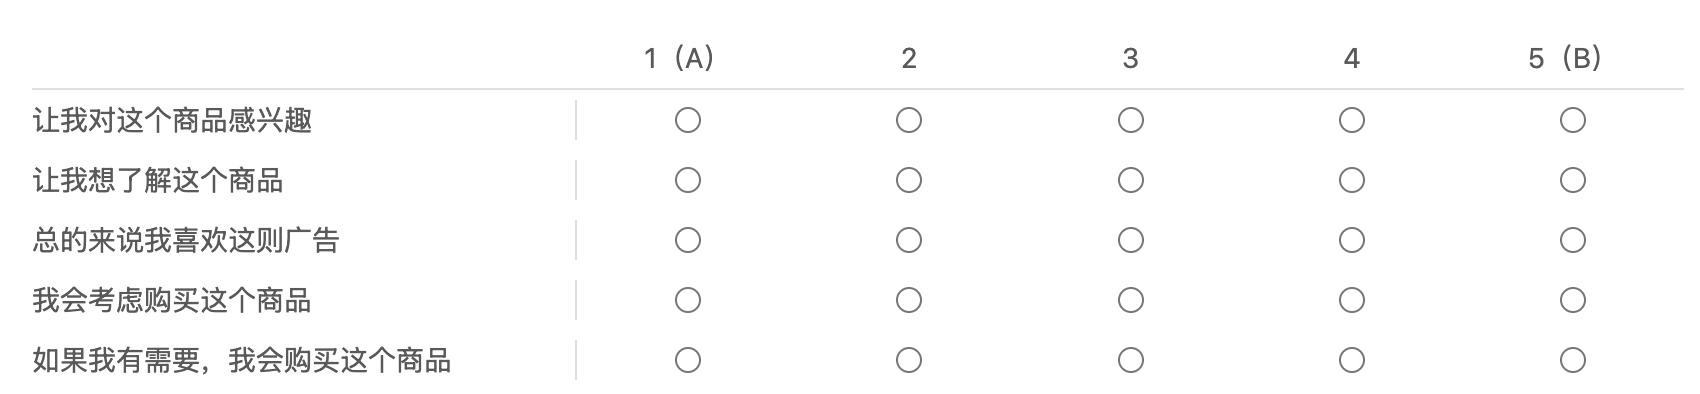
\includegraphics[width=.7\linewidth]{Image/Study1-exp2-rating.png}
    \caption{\label{fig:study1-exp2-rating-example}实验评分示意}
\end{figure}



\subsection{实验流程}
本实验的流程分为两个部分。第一部分,参与者依次阅读每组广告(个性化广告与中性广告并排呈现),并对每组广告的相对说服效果进行评分。广告呈现顺序随机化,以控制顺序效应。第二部分,参与者需回答与人格测试相关的问卷题目,最后提供年龄、性别等人口统计学信息。

\subsection{结果}
我们分别对尽责性个性化广告和开放性个性化广告进行了回归分析。回归模型的自变量包括参与者对应人格特质的得分(尽责性/开放性)、产品类型(电脑/薯片)以及特质与产品类型的交互项,因变量为广告的说服效果。由于评分为二极分布,我们对数据进行了转换,使得得分越高表示相较于中性广告,参与者对个性化广告的偏好越强。

针对尽责性个性化广告,回归模型如下: \begin{equation} Y_{\text{尽责性}} = \beta_0 + \beta_1 \cdot \text{尽责性特质} + \beta_2 \cdot \text{产品类型} + \beta_3 \cdot (\text{尽责性特质} \times \text{产品类型}) + \epsilon \end{equation}

回归分析结果显示,\textbf{尽责性特质的主效应显著}(\textit{$\beta$} = 0.3455, \textit{p} = 0.038),但产品类型的主效应(\textit{$\beta$} = 0.8079, \textit{p} > 0.05)和特质与产品类型的交互项(\textit{$\beta$} = -0.1372, \textit{p} > 0.05)均不显著。这表明,尽责性得分较高的个体相较于中性广告,更偏好针对高尽责性设计的个性化广告,但这种偏好不因产品类型而显著变化。

针对开放性个性化广告,回归模型如下: \begin{equation} Y_{\text{开放性}} = \beta_0 + \beta_1 \cdot \text{开放性特质} + \beta_2 \cdot \text{产品类型} + \beta_3 \cdot (\text{开放性特质} \times \text{产品类型}) + \epsilon \end{equation}

回归分析结果显示,\textbf{开放性特质的主效应显著}(\textit{$\beta$} = 0.3349, \textit{p} = 0.048),但产品类型的主效应(\textit{$\beta$} = -0.9128, \textit{p} > 0.05)和特质与产品类型的交互项(\textit{$\beta$} = 0.1851, \textit{p} > 0.05)均不显著。这表明,开放性得分较高的个体相较于中性广告,更偏好针对高开放性设计的个性化广告,同样,这种偏好不因产品类型的不同而显著变化。
\section{实验3:AI基于中性广告生成高低水平个性化广告的能力}

实验2验证了AI在不同产品类型的中性广告基础上生成个性化广告的能力,结果表明AI能够在享乐型与实用型产品中提取相应的个性化策略,并针对不同人格特质生成有效的个性化广告。然而,实验2仅关注了针对高水平人格特质(如高开放性、高尽责性)的个性化生成,未涉及低水平人格特质的定制设计。在实际应用中,广告不仅需要满足高水平特质个体的需求,还可能需要针对低水平特质个体进行设计,以覆盖更广泛的受众群体。

另一方面,针对高低水平人格特质的个性化效果,在现有文献中并未得到一致的验证。\citet{matz2017psychological}在其大样本实践研究中仅检验了开放性和外倾性分别针对高低水平设计的有效性,未涉及所有人格特质。而在\citet{matz2024potential}基于GPT生成个性化广告的研究中,不同实验间的结果也存在不一致性:部分实验中,针对高低水平设计的个性化广告在开放性、尽责性和外倾性维度上效果显著,但宜人性未能得到稳定的结果。同时,不同因变量(如广告效果与支付意愿)的测量中,高低水平的个性化效果差异也不稳定,尤其是外倾性维度,在某些实验中表现显著,而在另一些实验中则未表现出显著性。

基于上述研究的不一致性,以及实验2未覆盖低水平人格特质的局限,实验3旨在进一步探讨AI在双重人格水平(高水平与低水平)情境下生成个性化广告的能力,并验证高低水平特质的个性化效果是否存在显著差异。这不仅有助于完善现有文献中的空白,也为AI生成的个性化广告在更复杂场景中的应用提供可靠依据。但在本实验中我们不会涉及神经质特质的个性化设计,因为神经质的特性较为独特,其在低水平端的匹配信息(即针对情绪稳定性的设计)往往对高水平和低水平个体均具有吸引力 \citep{matz2016personality},因此难以实现真正针对高低水平的有效区分。


\subsection{方法}


\textbf{(1)被试}

通过见数平台发布实验,356名参与者自愿参加这项研究。36名参与者由于注意检查测试未通过被剔除,剩余\textbf{320名有效参与者}(年龄范围= 18-59岁;\textit{M}=26.06岁;\textit{SD}=7.90;女性200名)。参与任务的每名参与者获得1元人民币作为报酬。注意力检测包含两部分,分别嵌入在因变量测量和人格问卷中,以明确指令题形式呈现(如“请选2”)。参与者需在两道注意力检测题中均作答正确,方可被纳入有效数据样本。每名被试会随机分配到四个特质(开放性、尽责性、外倾性、宜人性)的条件之一,最终每个特质条件均有约80名被试参与。


\textbf{(2)实验材料:广告设计}

本实验共设计\textbf{2(水平:高/低)* 4(特质:开放性、尽责性、外倾性、宜人性)共8则个性化广告}。这些广告均基于一则来自微博平台的热门新款手机中性广告,通过GPT的文本生成与调整功能进行个性化设计。中性广告从当前热门的手机品牌官方广告中筛选而来,考虑到本实验的测量方式旨在比较不同的广告效果,因此品牌效应在比较中被抵消。同时,保留品牌信息能够增强广告的真实性和实验情境的生态效度,因此在本实验中未移除广告中的品牌信息。原广告示例如图\ref{fig:Study1-substudy3-originalAd}所示。针对每个特质与水平的组合,我们使用了GPT生成个性化广告文案(详见附录)。生成过程基于一套结构化的提示语(prompt),提示语(详见附录)包含以下关键要素:任务目标,原始广告文案,调整优化的要求,策略说明。为验证个性化广告的有效性,本研究在正式实验前通过见数平台发布了预实验,共有90名参与者自愿参加,并获得1元人民币作为报酬。每名参与者需对8则广告的目标消费者群体进行选择,具体任务为从2(水平)*5(特质)中选择出最匹配的目标消费者。预实验结果显示,大多数参与者能够正确识别出各广告的目标消费者特质,这表明GPT生成的个性化广告在针对特定人格特质的目标消费者设计上具有有效性。

\begin{figure}[H]
    \centering
    
\includegraphics[width=.8\linewidth]{Image/Study1-exp3-original ad.png}
    \caption{\label{fig:Study1-substudy3-originalAd}微博提取广告示意图}
\end{figure}



\textbf{(3)问卷测量}
\label{study1-substudy3-measures}

a. 大五人格量表
本实验从\citet{john1991big}编制的44道题目大五人格量表(BFI-44)中筛选出与目标特质相关的题目。参与者根据其被分配到的人格特质类别完成相应题目。每个题项采用1-5点李克特量表,1分表示“完全不符合”,5分表示“完全符合”。

b. 广告说服效果
实验中,高水平与低水平的个性化广告以并排形式随机呈现,分别标记为广告A和广告B。参与者需对两则广告的偏好进行评分,评分采用11点双极量表(如图\ref{fig:Study1-exp3-rating}),分值范围从“更倾向于广告A”到“更倾向于广告B”。为避免顺序效应,广告A/B呈现顺序随机化。为便于结果解读,在数据统计时将评分结果进行转换,使得分数越高表示参与者对高水平的个性化广告的偏好越强,分数越低表示参与者对低水平的个性化广告的偏好越强。

具体测量题项与实验2保持一致,共包括五个题项,分别评估参与者对广告和产品的态度及其购买意图。广告说服效果的总评分为五个题项得分的平均值。

c. 关键词选择
在广告说服效果评分完成后,参与者还需从每则广告中选出最吸引他们的Top3关键词。这些关键词用于后续分析,以进一步探讨个性化广告的有效性。例如,通过比较高水平与低水平广告中被选出的关键词,评估不同人格特质的参与者是否更倾向于关注与其特质匹配的广告要素。

\begin{figure}[H]
    \centering
    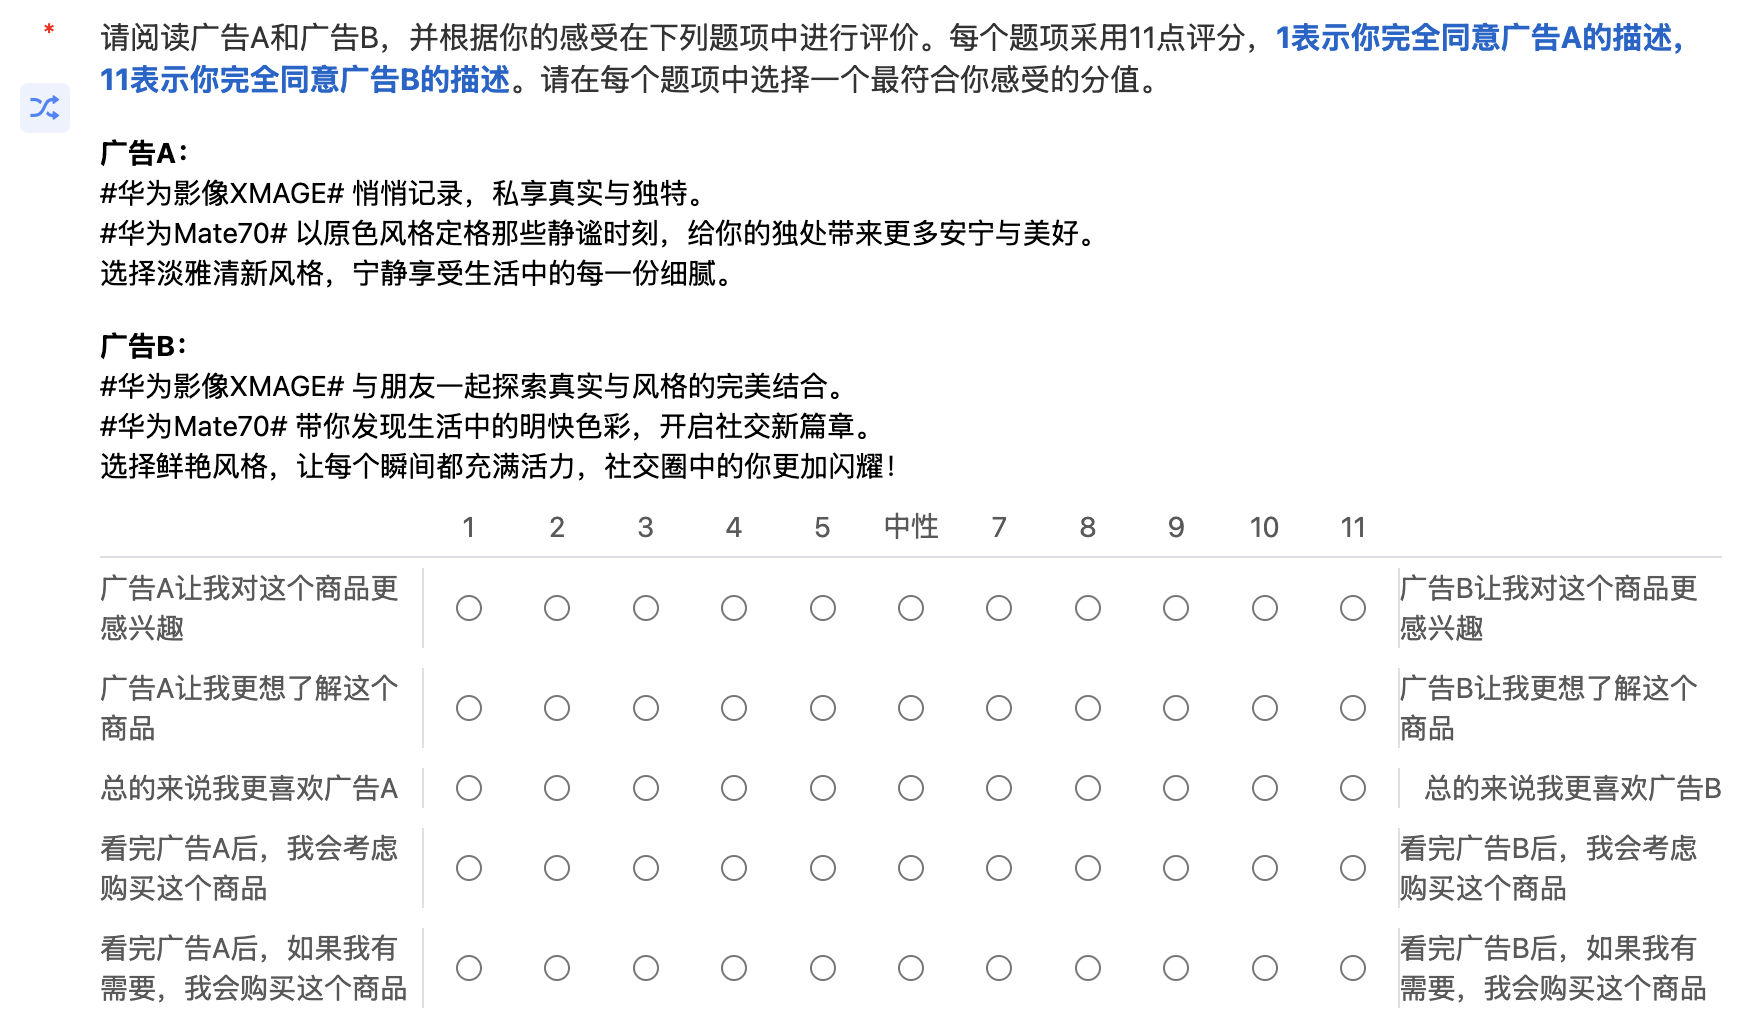
\includegraphics[width=.8\linewidth]{Image/Study1-exp3-rating.png}
    \caption{\label{fig:Study1-exp3-rating}实验评分示意}
\end{figure}


\subsection{实验流程}
本实验流程分为两个部分。第一部分,参与者依次阅读每组广告,其中每组广告包含高水平与低水平的个性化广告(例如,针对高外倾性和低外倾性设计的广告),并对每组广告的相对说服效果进行评分。第二部分,参与者完成与人格测试相关的问卷,随后填写包括年龄、性别等在内的人口统计学信息。

\subsection{结果}
我们分别对每个特质的结果进行了回归分析。回归模型的自变量为参与者对应人格特质的得分(尽责性、开放性、外倾性、宜人性),因变量为广告的说服效果。由于评分为二极分布,我们对数据进行了转换,使得得分越高表示相较于低水平个性化广告,参与者对高水平个性化广告的偏好越强。在这一模型中,如果存在匹配效应(即高水平特质的参与者更偏好针对高水平设计的个性化广告,而低水平特质的参与者更偏好针对低水平设计的个性化广告),则回归系数应为正且显著。

结果如图\ref{fig:Study1-exp3-result}所示,展示了针对四种人格特质设计的广告组的标准化效应及其95\%置信区间。结果表明,开放性(\textit{$\beta$} = 1.729,\textit{p} < 0.01)、外倾性(\textit{$\beta$} = 2.451,\textit{p} < 0.001)和宜人性(\textit{$\beta$} = 1.864,\textit{p} < 0.05)的得分显著预测了参与者对相应特质个性化广告的偏好。这意味着,在这些特质维度上,水平较高的参与者更偏好针对高水平设计的广告,水平较低的参与者则更偏好针对低水平设计的广告。然而,对于尽责性(\textit{$\beta$} = 0.101,\textit{p} = 0.898)维度,未观察到类似的匹配效应,表明无论是高尽责还是低尽责的参与者,在广告偏好上表现出相似的趋势。

\begin{figure}[H]
    \centering
    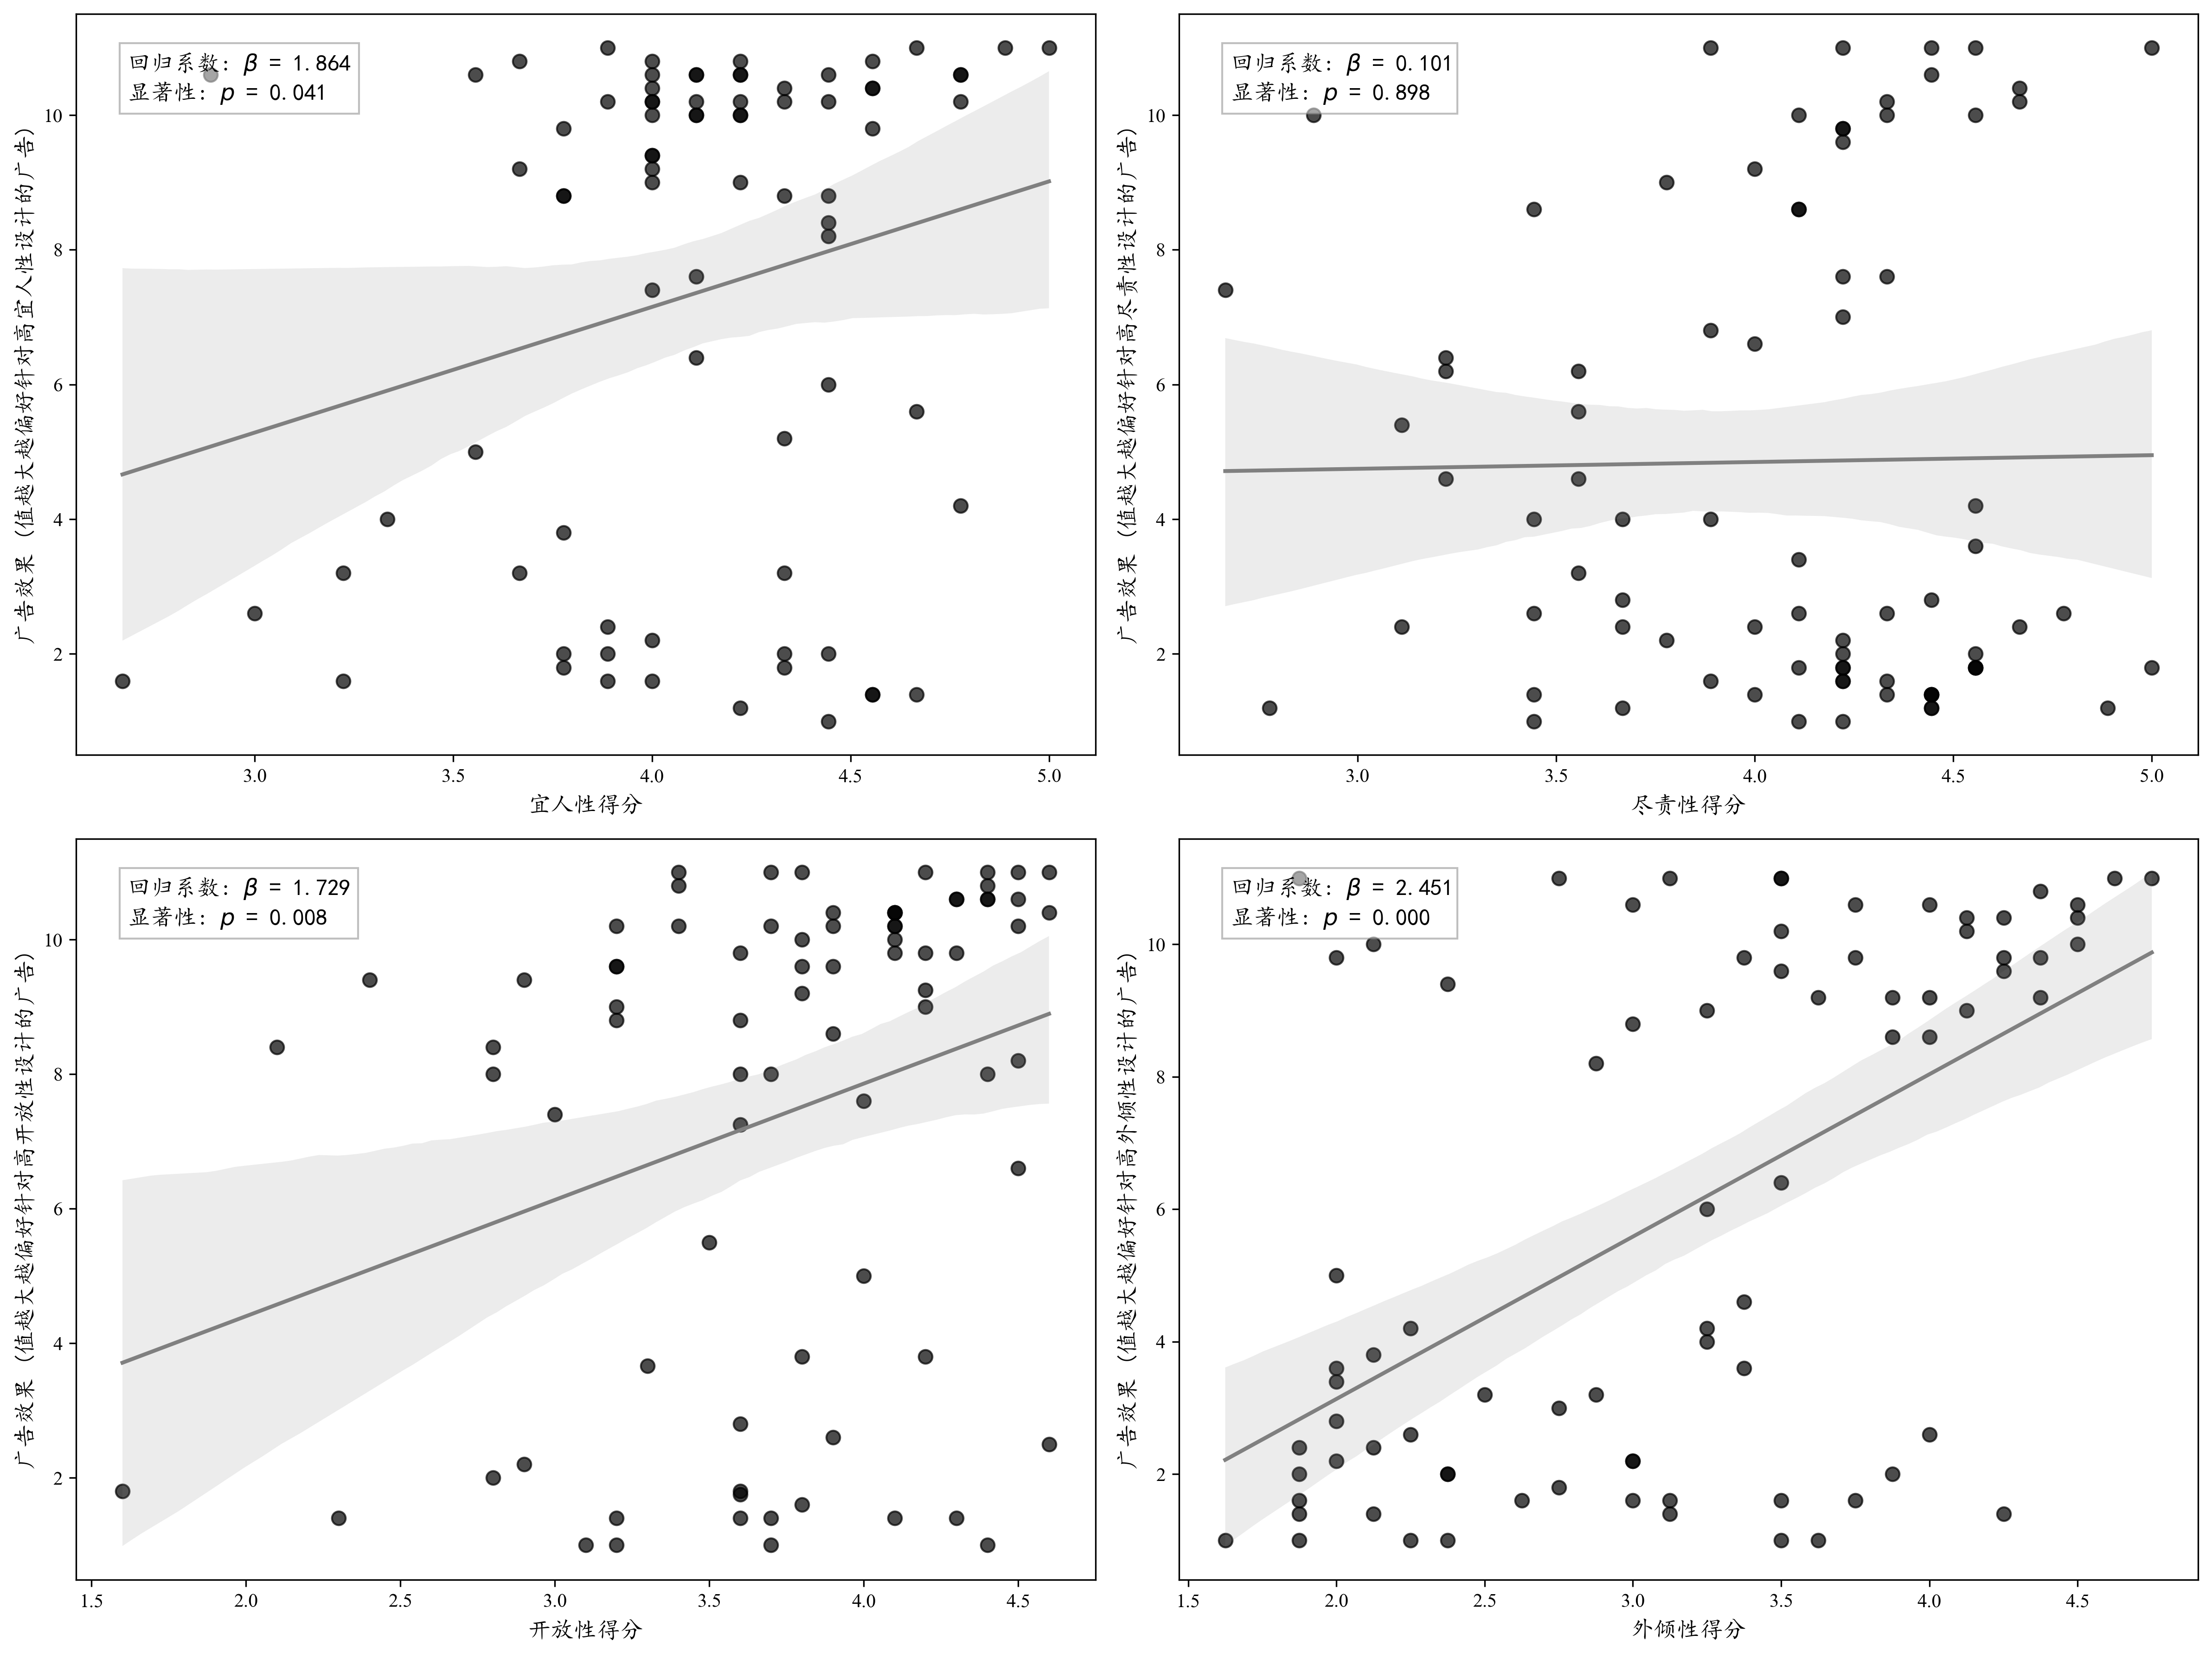
\includegraphics[width=1.0\linewidth]{Image/Study1-exp3-result.png}
    \caption{\label{fig:Study1-exp3-result}四个人格特质对相应广告效果评分的影响(含95\%置信区间)}
\end{figure}

为进一步探讨参与者偏好个性化广告的原因,我们将参与者按人格水平的中值划分为高水平组和低水平组,并筛选出他们在偏好广告中选择的Top 3关键词(根据广告说服效果评分,得分≥6表示更偏好针对高水平设计的广告,<6表示更偏好针对低水平设计的广告),对这些关键词进行词频统计和分析。这种方法能够揭示不同人格水平的个体在广告偏好上的差异,从而帮助解释个性化广告效果的背后机制。

针对回归分析中个性化效果显著的宜人性(表\ref{tab:agreeableness_neutrl_preference})、开放性(表\ref{tab:openness_neutral_preference})和外倾性特质(表\ref{tab:extraversion_neutral_preference}),词频统计结果表明,高水平个体在偏好广告中选择的关键词与广告设计的个性化特征高度一致。例如,在高开放性组中,频繁出现的关键词包括“探索创意”“开启视觉探险”“让想象力成为你的画布”“创新风格”等,这些词语正是针对高开放性设计时所突出的特征,表明个性化广告成功激发了高开放性个体的兴趣和共鸣。然而,对于尽责性特质,尽管回归结果未显示显著的个性化效果,但关键词分析揭示了一些有趣的现象(表\ref{tab:conscientiousness_neutral_preference})。高尽责性组的参与者在偏好广告中也频繁选择了一些针对低尽责性设计的词语,例如“轻松自在”(38.10\%)、“随性而行”(35.71\%)、“享受每一个自由的瞬间”(19.05\%)和“不受拘束”(19.05\%)。虽然这些词语确实也被低尽责性组的参与者广泛选择,但其在高尽责性组中的出现反映出某种交叉偏好。这一现象可能表明,尽责性特质在广告偏好中的表现受到其他特质的影响。例如,高尽责性个体如果同时具有高开放性特质,可能会对这些强调自由和创造性的词语产生共鸣。因此,可以推测当前针对尽责性设计的个性化广告特征还不够突出,导致在高尽责性组中未能显著区分出偏好差异。

综上所述,关键词分析不仅验证了个性化广告在宜人性、开放性和外倾性维度上的有效性,还揭示了尽责性维度个性化效果不显著的可能原因,即现有设计未能充分突出尽责性特质,且其他特质可能对广告偏好产生交互影响。


\definecolor{darkgreen}{RGB}{0,100,0} % 深绿色定义

\begin{table}[htbp]
    \centering
    \caption{\label{tab:agreeableness_neutrl_preference} 高宜人个体与低宜人个体广告词偏好}
    {\tablesongti % 整个表格环境应用宋体六号字体
    \renewcommand{\arraystretch}{1.5} % 调整行距
    \begin{tabularx}{\linewidth}{>{\raggedright\arraybackslash}X c >{\raggedright\arraybackslash}X c}
        \toprule
        \textbf{高宜人个体} & \textbf{比例} & \textbf{低宜人个体} & \textbf{比例} \\
        \midrule
        \textcolor{darkgreen}{捕捉那些充满爱与关怀的温馨瞬间} & \textcolor{darkgreen}{53.33\%} & 捕捉那些充满爱与关怀的温馨瞬间 & 34.29\% \\
        \textcolor{darkgreen}{体贴入微} & \textcolor{darkgreen}{40.00\%} & 体贴入微 & 31.43\% \\
        \textcolor{darkgreen}{让每个微笑都被温柔以待}& \textcolor{darkgreen} {26.67\%} & \textcolor{red}{个性鲜明} & \textcolor{red}{25.71\% }\\
        \textcolor{darkgreen}{你的生活增添和谐美好} & \textcolor{darkgreen} {24.44\%} & \textcolor{red}{独立自主} & \textcolor{red}{22.86\%} \\
        独立自主 & 22.22\% & 让每个微笑都被温柔以待 & 22.86\% \\
        \textcolor{darkgreen}{真诚记录每一次心动} & \textcolor{darkgreen} {20.00\%} & 关怀周到 & 20.00\% \\
        个性鲜明 & 13.33\% & 你的生活增添和谐美好 & 20.00\% \\
        \textcolor{darkgreen}{关怀周到} & \textcolor{darkgreen} {13.33\%} & \textcolor{red}{彰显自我} & \textcolor{red}{17.14\%} \\
        定格每一个独特视角 & 11.11\% & \textcolor{red}{定格每一个独特视角} & \textcolor{red}{17.14\%} \\
        彰显自我 & 6.67\% & 真诚记录每一次心动 & 14.29\% \\
        \bottomrule
    \end{tabularx}
    \vspace{0.1mm}
    \caption*{\raggedright \footnotesize 注:绿色为针对高宜人设计的词语特征,红色为针对低宜人设计的词语特征。}
    }
\end{table}

\begin{table}[htbp]
    \centering
    \caption{\label{tab:openness_neutral_preference} 高开放个体与低开放个体广告词偏好}
    {\tablesongti % 整个表格环境应用宋体六号字体
    \renewcommand{\arraystretch}{1.5} % 调整行距
    \begin{tabularx}{\linewidth}{>{\raggedright\arraybackslash}X c >{\raggedright\arraybackslash}X c}
        \toprule
        \textbf{高开放个体} & \textbf{比例} & \textbf{低开放个体} & \textbf{比例} \\
        \midrule
        \textcolor{darkgreen}{探索创意} & \textcolor{darkgreen}{52.27\%} & \textcolor{red}{经典永恒} & 38.89\% \\
        \textcolor{darkgreen}{开启视觉探险} & \textcolor{darkgreen}{43.18\%} & 探索创意 & 36.11\% \\
        \textcolor{darkgreen}{让想象力成为你的画布} & \textcolor{darkgreen}{38.64\%} & 开启视觉探险 & 33.33\% \\
        \textcolor{darkgreen}{创新风格} & \textcolor{darkgreen}{36.36\%} & 创新风格 & 30.56\% \\
        \textcolor{darkgreen}{无限可能} & \textcolor{darkgreen}{25.00\%} & \textcolor{red}{简单直接} & 30.56\% \\
        \textcolor{darkgreen}{每一次快门都是对未知的好奇} & \textcolor{darkgreen}{22.73\%} & 无限可能 & 22.22\% \\
        经典永恒 & 18.18\% & \textcolor{red}{享受熟悉的舒适} & \textcolor{red}{19.44\%} \\
        简单直接 & 9.09\% & 每一次快门都是对未知的好奇 & 13.89\% \\
        坚持你的风格 & 6.82\% & 让想象力成为你的画布 & 13.89\% \\
        享受熟悉的舒适 & 4.55\% & \textcolor{red}{信赖已知} & \textcolor{red}{13.89\%} \\
        信赖已知 & 2.27\% & \textcolor{red}{坚持你的风格} & \textcolor{red}{5.56\%} \\
        \bottomrule
    \end{tabularx}
    \vspace{0.1mm}
    \caption*{\raggedright \footnotesize 注:绿色为针对高开放设计的词语特征,红色为针对低开放设计的词语特征。}
    
    }
\end{table}

\begin{table}[H]
    \centering
    \caption{\label{tab:extraversion_neutral_preference} 高外倾个体与低外倾个体广告词偏好}
    {\tablesongti % 整个表格环境应用宋体六号字体
    \renewcommand{\arraystretch}{1} % 调整行距
    \begin{tabularx}{\linewidth}{>{\raggedright\arraybackslash}X c >{\raggedright\arraybackslash}X c}
        \toprule
        \textbf{高外倾个体} & \textbf{比例} & \textbf{低外倾个体} & \textbf{比例} \\
        \midrule
        \textcolor{darkgreen}{让每个瞬间都充满活力} & \textcolor{darkgreen}{39.02\%} & \textcolor{red}{私享真实与独特} & \textcolor{red}{46.15\%} \\
        \textcolor{darkgreen}{带你发现生活中的明快色彩} & \textcolor{darkgreen}{31.71\%} & \textcolor{red}{给你的独处带来更多安宁与美好} & \textcolor{red}{41.03\%} \\
        私享真实与独特 & 26.83\% & \textcolor{red}{宁静享受生活中的每一份细腻} & \textcolor{red}{30.77\%} \\
        \textcolor{darkgreen}{开启社交新篇章} & \textcolor{darkgreen}{24.39\%} & \textcolor{red}{定格那些静谧时刻} & \textcolor{red}{28.21\%} \\
        \textcolor{darkgreen}{社交圈中的你更加闪耀} & \textcolor{darkgreen}{24.39\%} & 让每个瞬间都充满活力 & 10.26\% \\
        宁静享受生活中的每一份细腻 & 17.07\% & \textcolor{red}{悄悄记录} & \textcolor{red}{10.26\%} \\
        \textcolor{darkgreen}{与朋友一起探索} & \textcolor{darkgreen}{12.20\%} & 带你发现生活中的明快色彩 & 7.69\% \\
        给你的独处带来更多安宁与美好 & 12.20\% & 社交圈中的你更加闪耀 & 5.13\% \\
        定格那些静谧时刻 & 4.88\% & 与朋友一起探索 & 5.13\% \\
        悄悄记录 & 2.44\% & 开启社交新篇章 & 2.56\% \\
        \bottomrule
    \end{tabularx}
    \vspace{0.1mm}
    \caption*{\raggedright \footnotesize 注:绿色为针对高外倾设计的词语特征,红色为针对低外倾设计的词语特征。}
    }
\end{table}


\begin{table}[H]
    \centering
    \caption{\label{tab:conscientiousness_neutral_preference} 高尽责个体与低尽责个体广告词偏好}
    {\tablesongti % 整个表格环境应用宋体六号字体
    \renewcommand{\arraystretch}{1} % 调整行距
    \begin{tabularx}{\linewidth}{>{\raggedright\arraybackslash}X c >{\raggedright\arraybackslash}X c}
        \toprule
        \textbf{高尽责个体} & \textbf{比例} & \textbf{低尽责个体} & \textbf{比例} \\
        \midrule
        \textcolor{darkgreen}{专业可靠} & \textcolor{darkgreen}{38.10\%} & \textcolor{red}{轻松自在} & \textcolor{red}{36.84\%} \\
        轻松自在 & 38.10\% & \textcolor{red}{享受每一个自由的瞬间} & \textcolor{red}{26.32\%}\\
        让每一天都活泼非凡 & 35.71\% & \textcolor{red}{随心选择色彩} & \textcolor{red}{23.68\%} \\
        随性而行 & 35.71\% & \textcolor{red}{随性而行} & \textcolor{red}{21.05\%} \\
        享受每一个自由的瞬间 & 19.05\% & 专业可靠 & 18.42\% \\
        不受拘束 & 19.05\% & 每个细节都尽善尽美 & 18.42\% \\
        \textcolor{darkgreen}{工作效率} & \textcolor{darkgreen}{14.29\%} & 让每一天都活泼非凡 & 18.42\% \\
        \textcolor{darkgreen}{准确无误} & \textcolor{darkgreen}{11.90\%} & 记录生活 & 15.79\% \\
        \textcolor{darkgreen}{每一个专业细节} & \textcolor{darkgreen}{11.90\%} & 准确无误 & 13.16\% \\
        随心选择色彩 & 7.14\% & 每一个专业细节 & 13.16\% \\
        \textcolor{darkgreen}{每个细节都尽善尽美} & \textcolor{darkgreen}{7.14\%} & \textcolor{red}{不受拘束} & \textcolor{red}{10.53\%} \\
        \textcolor{darkgreen}{精准捕捉} & \textcolor{darkgreen}{7.14\%} & 工作效率 & 10.53\% \\
        \textcolor{darkgreen}{增添工作的效率与精确} & \textcolor{darkgreen}{7.14\%} & 精准捕捉 & 10.53\% \\
        记录生活 & 2.38\% & 增添工作的效率与精确 & 5.26\% \\
        \bottomrule
    \end{tabularx}
    \vspace{0.1mm}
    \caption*{\raggedright \footnotesize 注:绿色为针对高尽责设计的词语特征,红色为针对低尽责设计的词语特征。}
    }
\end{table}


\section{实验4:AI基于产品描述生成高低水平个性化广告的能力}

实验3验证了AI在中性广告基础上,针对高水平和低水平人格特质生成个性化广告的能力,结果显示在开放性、外倾性和宜人性三个维度上,AI能够有效生成符合不同人格特质水平的个性化广告。然而,在尽责性维度上,并未观察到显著的匹配效应,这可能与尽责性特质的内在特性有关,或与现有中性广告的基础信息不足,难以准确区分高低尽责性的偏好有关。

尽管实验3证明了AI在已有中性广告基础上调整生成个性化广告的能力,但实际广告创作中,尤其是针对新品或特定市场推广场景,往往缺乏现成的中性广告作为基础。在这些情境下,品牌通常需要基于产品描述直接创作广告内容。因此,实验4旨在进一步探讨AI是否能够基于产品描述直接生成针对不同人格特质的个性化广告,从而验证其在更复杂应用场景下的个性化生成能力。

此外,相较于实验3基于已有广告的微调生成,实验4的任务要求更高,AI不仅需要理解产品描述的核心信息,还需要准确提取与目标人格特质相关的要素,进而生成符合特定人格偏好的广告内容。因此,实验4的研究将进一步扩展AI生成个性化广告的适用范围,验证其生成高效个性化广告的能力。

\subsection{方法}


\textbf{(1)被试}

通过见数平台发布实验,368名参与者自愿参加这项研究。48名参与者由于注意检查测试未通过被剔除,剩余\textbf{320名有效参与者}(年龄范围= 18-57岁;\textit{M}=25.88岁;\textit{SD}=6.30;女性198名)。参与任务的每名参与者获得1元人民币作为报酬。注意力检测包含两部分,分别嵌入在因变量测量和人格问卷中,以明确指令题形式呈现(如“请选2”)。参与者需在两道注意力检测题中均作答正确,方可被纳入有效数据样本。每名被试会随机分配到四个特质(开放性、尽责性、外倾性、宜人性)的条件之一,最终每个特质条件均有约80名被试参与。


\textbf{(2)实验材料:广告设计}

实验材料生成数量与实验3一致,共设计\textbf{2(水平:高/低)* 4(特质:开放性、尽责性、外倾性、宜人性)共8则个性化广告}。与实验3不同,实验4中的个性化广告不是基于现有的中性广告进行调整,而是直接基于产品描述生成。我们选择了与实验3相同的产品,即华为Mate70,为了确保生成内容的真实性与关联性,我们从百度搜索中找到的第一篇华为Mate70亮点介绍网页中提取了主要产品特性作为输入内容。针对每个特质与水平的组合,我们使用GPT4生成个性化广告文案。生成过程基于一套结构化提示词(详见附录),包含任务目标、产品描述、调整与优化要求、策略说明。具体而言,GPT的任务是根据输入的产品描述,结合高/低水平的目标人格特质,生成针对目标消费者的个性化广告文案(详见附录)。

为验证生成的个性化广告是否能够有效传达针对目标消费者的特质,本研究在正式实验前通过见数平台发布了预实验,共有90名参与者自愿参加,并获得1元人民币作为报酬。每名参与者需阅读8则广告,并从2(水平)* 5(特质描述)中选择出最匹配的目标消费者。预实验结果表明,大多数参与者能够正确识别出广告所针对的人格特质,这表明GPT基于产品描述生成的个性化广告在针对特定人格特质的目标消费者设计上具有有效性。


\textbf{(3)问卷测量}

同实验3(详见\ref{study1-substudy3-measures},分别测量广告说服效果和大五人格量表。


\subsection{实验流程}
本实验流程分为两个部分。第一部分,参与者依次阅读每组广告,其中每组广告包含高水平与低水平的个性化广告(例如,针对高外倾性和低外倾性设计的广告),并对每组广告的相对说服效果进行评分。第二部分,参与者完成与人格测试相关的问卷,随后填写包括年龄、性别等在内的人口统计学信息。

\subsection{结果}
我们分别对每个特质的结果进行了回归分析。回归模型的自变量为参与者对应人格特质的得分(尽责性、开放性、外倾性、宜人性),因变量为广告的说服效果。由于评分为二极分布,我们对数据进行了转换,使得得分越高表示相较于低水平个性化广告,参与者对高水平个性化广告的偏好越强。在这一模型中,如果存在匹配效应(即高水平特质的参与者更偏好针对高水平设计的个性化广告,而低水平特质的参与者更偏好针对低水平设计的个性化广告),则回归系数应为正且显著。

结果如图\ref{fig:Study1-exp3-result}所示,展示了针对四种人格特质设计的广告组的标准化效应及其95\%置信区间。结果显示,仅在开放性(\textit{$\beta$} = 1.896,\textit{p} < 0.01)和外倾性(\textit{$\beta$} = 2.366,\textit{p} < 0.001)维度上观察到显著的个性化效果,即高开放性和高外倾性的个体更偏好针对高水平特质设计的广告,而低开放性和低外倾性的个体则更偏好针对低水平特质设计的广告。在宜人性维度(\textit{$\beta$} = 0.687,\textit{p} = 0.490)上,未发现显著的个性化效果,表明高低宜人性个体在广告偏好上无明显差异。值得注意的是,在尽责性维度上,回归结果呈现出负向的个性化效果(\textit{$\beta$} = -1.721,\textit{p} < 0.05),即高尽责性个体更偏好针对低尽责性设计的广告,而低尽责性个体则更偏好针对高尽责性设计的广告。

\begin{figure}[H]
    \centering
    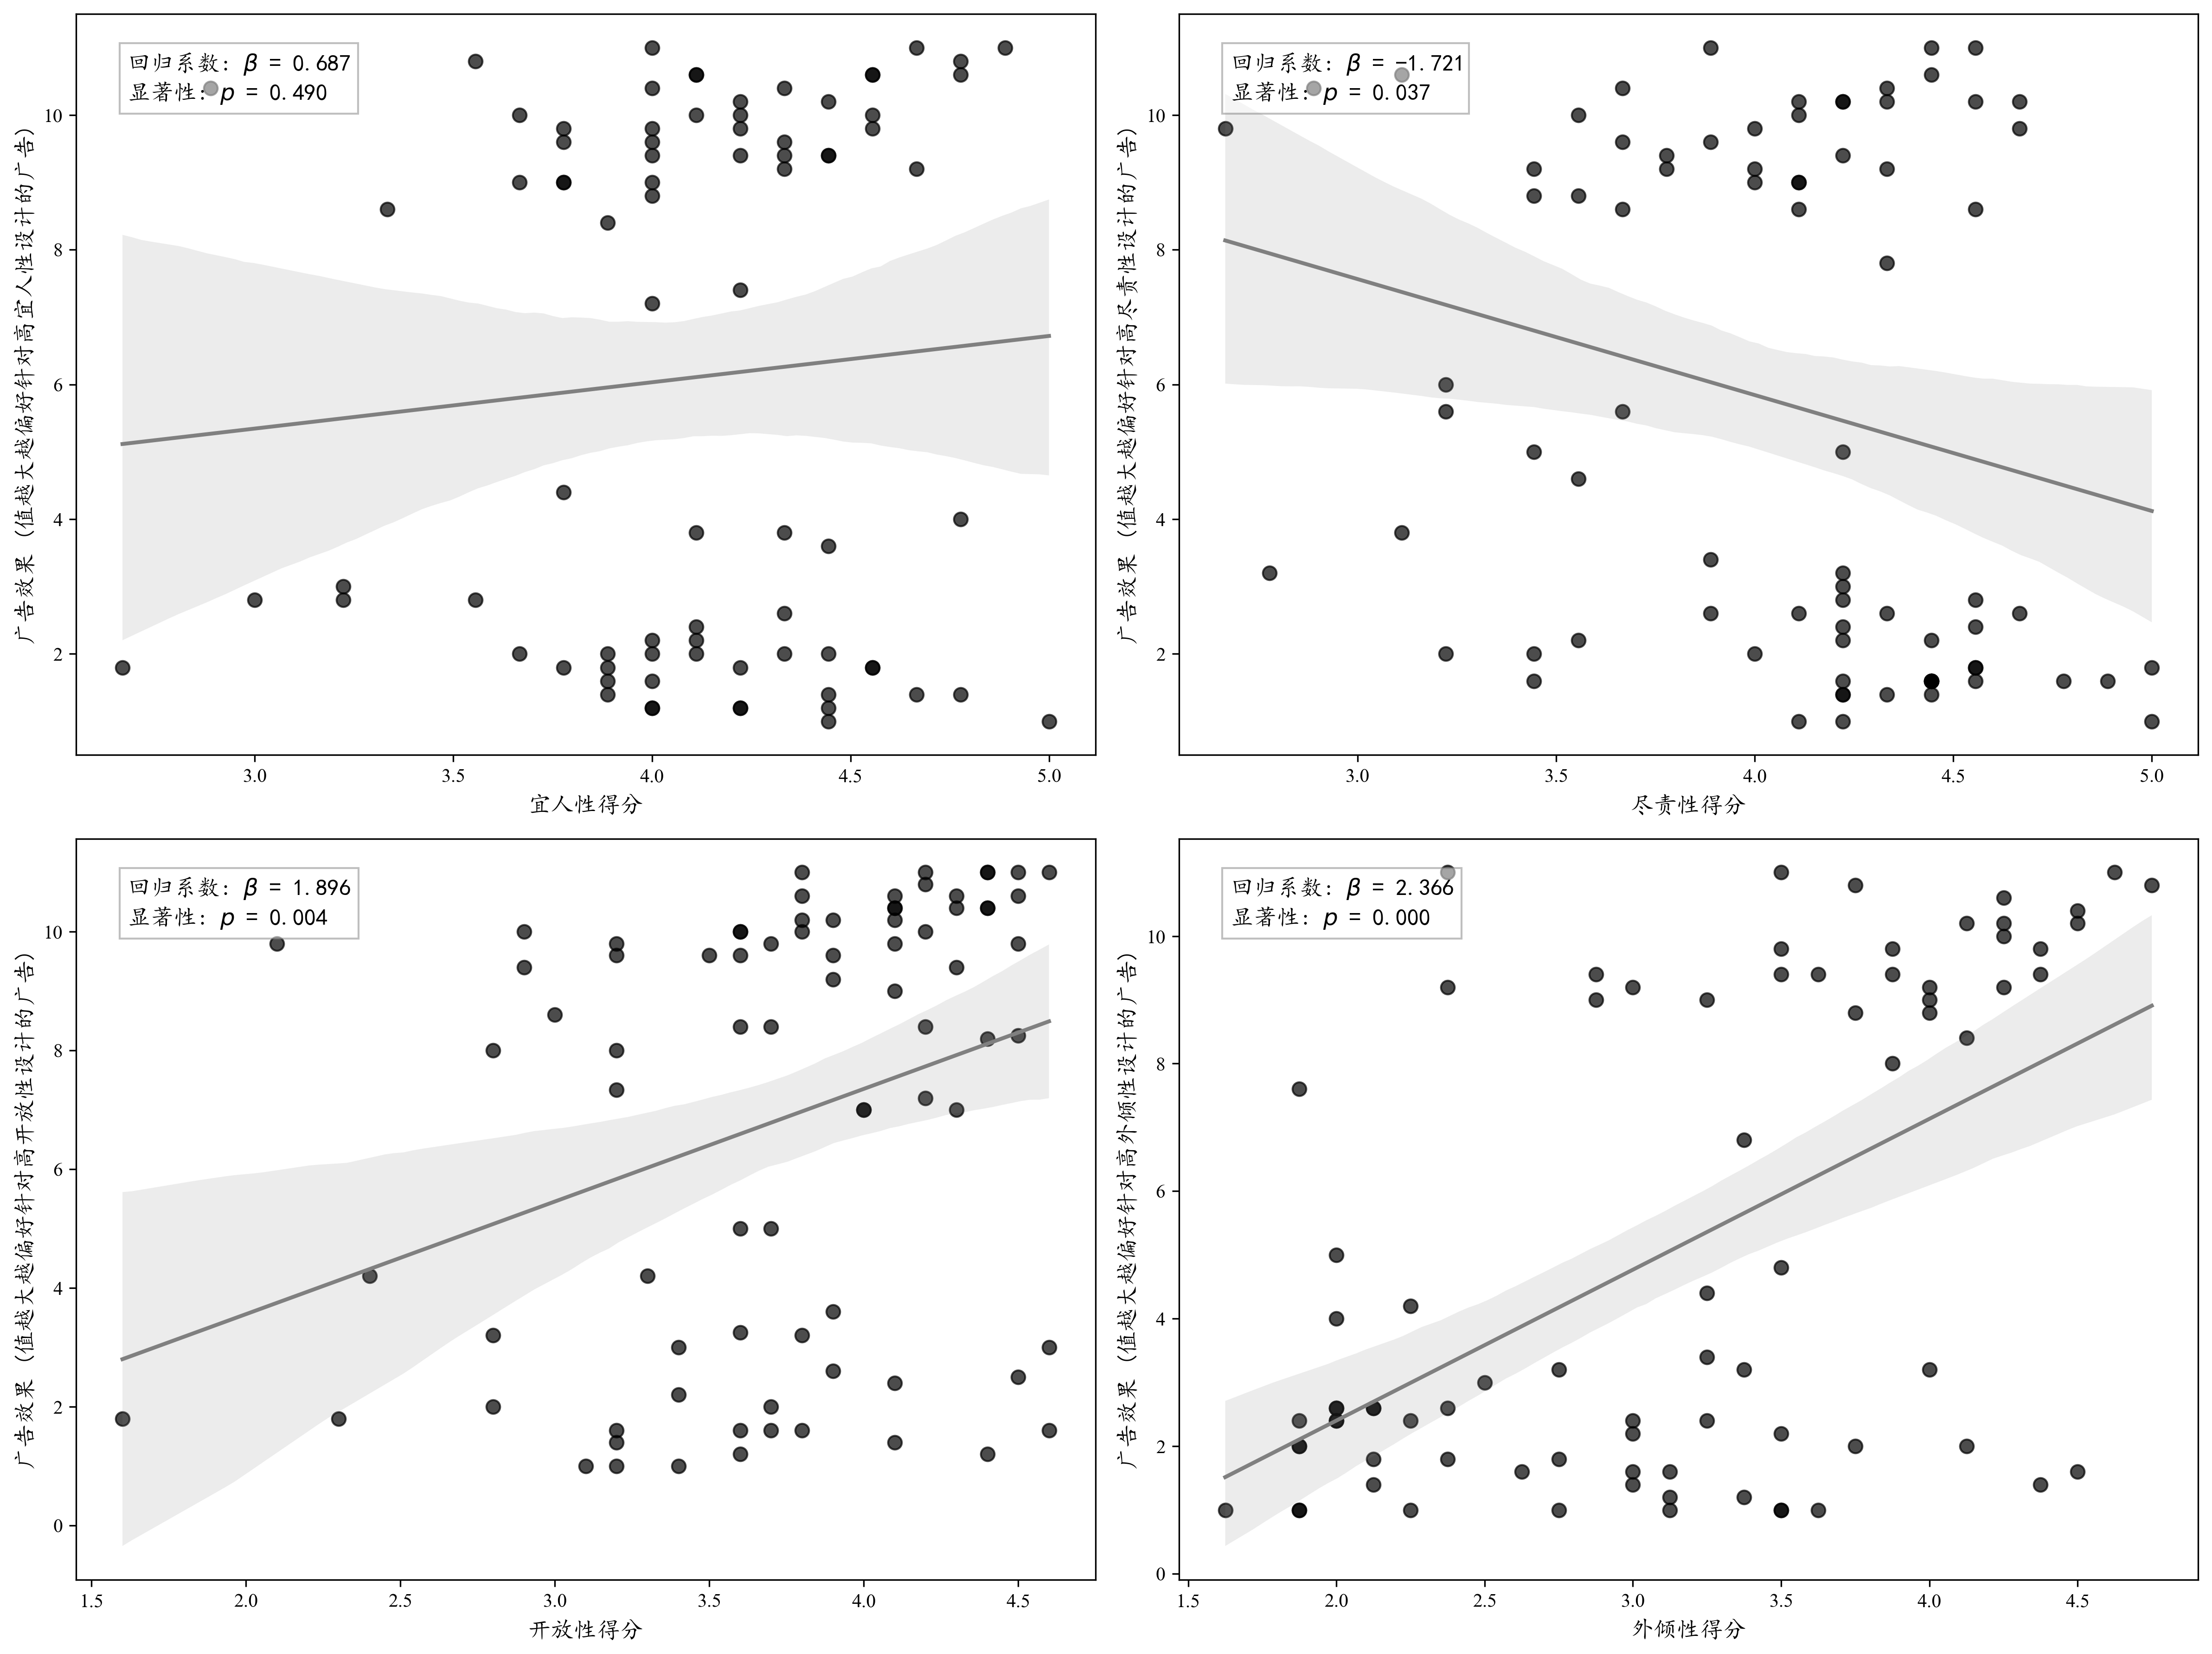
\includegraphics[width=1.0\linewidth]{Image/Study1-exp4-result.png}
    \caption{\label{fig:Study1-exp4-result}四个人格特质对相应广告效果评分的影响(含95\%置信区间)}
\end{figure}

与实验3相同,为进一步探讨参与者偏好个性化广告的原因,我们通过参与者选择的吸引他们的关键词进行分析。对于回归分析中个性化效果显著的开放性和外倾性维度,关键词特征分析结果与个性化设计方向一致。

如表\ref{tab:openness_product_preference}所示,在开放性维度上,高开放性个体偏好的Top关键词包括“无畏创新”(70.45%)、“创意P图”(45.45%)和“探索未知”(43.18%),这些词语正是针对高开放性设计时突出的特征。而低开放性个体偏好的Top关键词为“抗衰耐用”(44.44%)、“简单又可靠”(38.89%)和“创意P图功能”(36.11%),其中前两个词语是针对低开放性设计的特征,而“创意P图功能”则是广告中常见的功能性亮点,因此受到不同类型个体的广泛关注。

如表\ref{tab:extraversion_product_preference}所示,在外倾性维度上,高外倾性个体偏好的Top关键词包括“颜值在线”(36.59\%)、“出场都是焦点”(26.83\%)和“全场瞩目必备”(17.07\%),这些词语明显强调了外倾性个体关注的社交形象和外在表现,与高外倾性个性化设计一致。而低外倾性个体偏好的Top关键词前三位主要为功能性词语,接下来的关键词“无干扰”(23.08\%)、“助力你的个人空间”(23.08\%)和“安静中自由天地”(20.51\%)则与低外倾性特质匹配,突出其对安静和隐私的需求。

对于个性化效果未达到显著水平的宜人性维度(表 \ref{tab:agreeableness_product_preference}),结果呈现出有趣的现象。关键词“充满理解与关怀”(针对高宜人设计,44.44\%)更多被低宜人性个体选择(48.57\%),而“真诚相待”这一针对高宜人设计的词语在低宜人性个体中排名最高(28.57\%)。这表明,在宜人性维度上,个性化设计未能显著区分高低宜人性个体的偏好,可能是由于高低宜人性个体在广告偏好上的差异较小。

对于回归结果呈现负向个性化效果的尽责性维度(表 \ref{tab:conscientiousness_product_preference}),关键词分析结果进一步揭示了这一现象背后的可能原因。一些针对低尽责性设计的关键词,如“简单享受”和“随性而为”,在高尽责性个体中反而被频繁选择,表明这些词语对高尽责性个体也具有吸引力。此外,针对高尽责性设计的关键词,如“100\%信号强度”和“每个细节都完美无瑕”,在低尽责性个体中更受欢迎。这一结果与实验3类似,可能是由于这些词语与开放性特质存在一定的关联性,导致高开放性个体在高尽责性组中对这些词语表现出偏好。

此外,为进一步理解实验中尽责性和宜人性维度未能呈现预期效果的原因,我们参考了先前研究中收集的5110名参与者的人格数据分布(图\ref{fig:Study1-exp4-distribution})。比较发现,本研究中(浅色)宜人性和尽责性维度的分布在高分段聚集了更多被试,这意味着我们的样本中高尽责性和高宜人性个体的比例较高。这一分布特性可能导致偏好上的内部差异性被放大,从而影响了高低水平组的区分效果。例如,在尽责性维度上,高水平组中可能包含了一些具有高开放性特质的个体,而开放性与“简单享受”“随性而为”等词语高度相关,因此这些词语即使针对低尽责性设计,也会被部分高尽责性个体偏好。同样,在宜人性维度上,高水平组内部可能存在更多异质性,导致高宜人性个体未能表现出一致的偏好。因此,数据分布的偏向性可能是导致尽责性和宜人性维度个性化效果未达预期的重要原因。这一结果提示未来研究在划分高低水平组时,应结合更大规模的标准化样本进行比较,或采用连续性指标而非简单的中位数划分,以提高高低水平组的区分精度,进而更准确地检验个性化广告效果。

\begin{table}[H]
    \centering
    \caption{\label{tab:agreeableness_product_preference} 高宜人个体与低宜人个体广告词偏好}
    {\tablesongti % 整个表格环境应用宋体六号字体
    \renewcommand{\arraystretch}{1} % 调整行距
    \begin{tabularx}{\linewidth}{>{\raggedright\arraybackslash}X c >{\raggedright\arraybackslash}X c}
        \toprule
        \textbf{高宜人个体} & \textbf{比例} & \textbf{低宜人个体} & \textbf{比例} \\
        \midrule
        \textcolor{darkgreen}{充满理解与关怀} & \textcolor{darkgreen}{44.44\%} & 充满理解与关怀 & 48.57\% \\
        \textcolor{darkgreen}{用心沟通} & \textcolor{darkgreen}{35.56\%} & \textcolor{red}{AI防窥功能} & \textcolor{red}{31.43\%} \\
        \textcolor{darkgreen}{真诚相待} & \textcolor{darkgreen}{35.56\%} & 真诚相待 & 28.57\% \\
        \textcolor{darkgreen}{不惧真我} & \textcolor{darkgreen}{31.11\%} & \textcolor{red}{保护你的隐私} & \textcolor{red}{28.57\%} \\
        AI防窥功能 & 28.89\% & \textcolor{red}{敢于直言} & \textcolor{red}{25.71\%} \\
        实时AI翻译功能 & 22.22\% & 实时AI翻译功能 & 22.86\% \\
        敢于直言 & 17.78\% & \textcolor{red}{独立自主} & \textcolor{red}{22.86\%} \\
        \textcolor{darkgreen}{保护你的隐私} & \textcolor{darkgreen}{15.56\%} & \textcolor{red}{不惧真我} & \textcolor{red}{20.00\%} \\
        独立自主 & 15.56\% & 用心沟通 & 20.00\% \\
        \textcolor{darkgreen}{温暖科技} & \textcolor{darkgreen}{13.33\%} & 温暖科技 & 11.43\% \\
        \textcolor{darkgreen}{只属于你自己} & \textcolor{darkgreen}{8.89\%} & \textcolor{red}{只属于你自己} & \textcolor{red}{11.43\%} \\
        \bottomrule
    \end{tabularx}
    \vspace{0.1mm}
    \caption*{\raggedright \footnotesize 注:绿色为针对高宜人设计的词语特征,红色为针对低宜人设计的词语特征。}
    }
\end{table}


\begin{table}[H]
    \centering
    \caption{\label{tab:openness_product_preference} 高开放个体与低开放个体广告词偏好}
    {\tablesongti % 整个表格环境应用宋体六号字体
    \renewcommand{\arraystretch}{1} % 调整行距
    \begin{tabularx}{\linewidth}{>{\raggedright\arraybackslash}X c >{\raggedright\arraybackslash}X c}
        \toprule
        \textbf{高开放个体} & \textbf{比例} & \textbf{低开放个体} & \textbf{比例} \\
        \midrule
        \textcolor{darkgreen}{无畏创新} & \textcolor{darkgreen}{70.45\%} & \textcolor{red}{抗摔耐用} & \textcolor{red}{44.44\%} \\
        \textcolor{darkgreen}{创意P图功能} & \textcolor{darkgreen}{45.45\%} & \textcolor{red}{简单又可靠} & \textcolor{red}{38.89\%} \\
        \textcolor{darkgreen}{探索未知} & \textcolor{darkgreen}{43.18\%} & 创意P图功能 & 36.11\% \\
        AI识别 & 22.73\% & AI识别 & 33.33\% \\
        \textcolor{darkgreen}{创意无限} & \textcolor{darkgreen}{20.45\%} & \textcolor{red}{熟悉的经典} & \textcolor{red}{30.56\%} \\
        \textcolor{darkgreen}{激发你的每一个创新想法} & \textcolor{darkgreen}{15.91\%} & 无畏创新 & 27.78\% \\
        \textcolor{darkgreen}{抗摔耐用} & \textcolor{darkgreen}{13.64\%} & \textcolor{red}{让生活更省心} & \textcolor{red}{19.44\%} \\
        简单又可靠 & 13.64\% & 探索未知 & 16.67\% \\
        让生活更省心 & 9.09\% & \textcolor{red}{稳定生活好选择} & \textcolor{red}{11.11\%} \\
        熟悉的经典 & 9.09\% & 轻松应对 & 8.33\% \\
        性能提升 & 6.82\% & 创意无限 & 5.56\% \\
        轻松应对 & 4.55\% & 性能提升 & 5.56\% \\
        & & 每一天的琐碎小事 & 2.78\% \\
        & & 激发你的每一个创新想法 & 2.78\% \\
        \bottomrule
    \end{tabularx}
    \vspace{0.1mm}
    \caption*{\raggedright \footnotesize 注:绿色为针对高开放设计的词语特征,红色为针对低开放设计的词语特征。}
    }
\end{table}

\begin{table}[H]
    \centering
    \caption{\label{tab:extraversion_product_preference} 高外倾个体与低外倾个体广告词偏好}
    {\tablesongti % 整个表格环境应用宋体六号字体
    \renewcommand{\arraystretch}{1} % 调整行距
    \begin{tabularx}{\linewidth}{>{\raggedright\arraybackslash}X c >{\raggedright\arraybackslash}X c}
        \toprule
        \textbf{高外倾个体} & \textbf{比例} & \textbf{低外倾个体} & \textbf{比例} \\
        \midrule
        \textcolor{darkgreen}{颜值在线} & \textcolor{darkgreen}{36.59\%} & AI P图随心创作 & 56.41\% \\
        \textcolor{darkgreen}{出场都是焦点} & \textcolor{darkgreen}{26.83\%} & 零束缚 & 30.77\% \\
        AI P图随心创作 & 26.83\% & 强悍性能 & 28.21\% \\
        无干扰 & 17.07\% & \textcolor{red}{无干扰} & \textcolor{red}{23.08\%} \\
        \textcolor{darkgreen}{全场瞩目必备} & \textcolor{darkgreen}{17.07\%} & \textcolor{red}{助力你的个人空间} & \textcolor{red}{23.08\%} \\
        \textcolor{darkgreen}{让你的社交不再有障碍} & \textcolor{darkgreen}{14.63\%} & 随时捕捉灵感 & 23.08\% \\
        零束缚 & 14.63\% & \textcolor{red}{让你沉浸在属于自己的世界} & \textcolor{red}{20.51\%} \\
        开放式AI翻译 & 12.20\% & \textcolor{red}{安静中自有天地} & \textcolor{red}{20.51\%} \\
        随时捕捉灵感 & 7.32\% & 独处的美好 & 12.82\% \\
        \textcolor{darkgreen}{社交达人首选} & \textcolor{darkgreen}{7.32\%} & 让你的社交不再有障碍 & 7.69\% \\
        强悍性能 & 7.32\% & 开放式AI翻译 & 5.13\% \\
        助力你的个人空间 & 7.32\% & 颜值在线 & 2.56\% \\
        独处的美好 & 4.88\% & 出场都是焦点 & 2.56\% \\
        \textcolor{darkgreen}{让你沉浸在属于自己的世界} & \textcolor{darkgreen}{4.88\%} & 社交达人首选 & 2.56\% \\
        & & 全场瞩目必备 & 2.56\% \\
        \bottomrule
    \end{tabularx}
    \vspace{0.1mm}
    \caption*{\raggedright \footnotesize 注:绿色为针对高外倾设计的词语特征,红色为针对低外倾设计的词语特征。}
    }
\end{table}

\begin{table}[H]
    \centering
    \caption{\label{tab:conscientiousness_product_preference} 高尽责个体与低尽责个体广告词偏好}
    {\tablesongti % 整个表格环境应用宋体六号字体
    \renewcommand{\arraystretch}{1} % 调整行距
    \begin{tabularx}{\linewidth}{>{\raggedright\arraybackslash}X c >{\raggedright\arraybackslash}X c}
        \toprule
        \textbf{高尽责个体} & \textbf{比例} & \textbf{低尽责个体} & \textbf{比例} \\
        \midrule
        简单享受 & 47.62\% & 100\%信号强度 & 44.74\% \\
        便捷的AI功能 & 28.57\% & 每个细节都完美无瑕 & 42.11\% \\
        随性而为 & 26.19\% & 40\%性能提升 & 39.47\% \\
        \textcolor{darkgreen}{100\%信号强度} & \textcolor{darkgreen}{26.19\%} & 为追求卓越而生 & 28.95\% \\
        \textcolor{darkgreen}{每个细节都完美无瑕} & \textcolor{darkgreen}{23.81\%} & 强悍性能 & 26.32\% \\
        \textcolor{darkgreen}{强悍性能} & \textcolor{darkgreen}{21.43\%} & \textcolor{red}{简单享受} & \textcolor{red}{26.32\%} \\
        \textcolor{darkgreen}{40\%性能提升} & \textcolor{darkgreen}{21.43\%} & 便捷的AI功能 & 21.05\% \\
        \textcolor{darkgreen}{为追求卓越而生} & \textcolor{darkgreen}{14.29\%} & \textcolor{red}{随性而为} & \textcolor{red}{15.79\%} \\
        随时随地 & 11.90\% & \textcolor{red}{轻松生活} & \textcolor{red}{15.79\%} \\
        想怎么用就怎么用 & 9.52\% & \textcolor{red}{随时随地} & \textcolor{red}{10.53\%} \\
        轻松生活 & 9.52\% & 专业人士 & 7.89\% \\
        \textcolor{darkgreen}{专业人士} & \textcolor{darkgreen}{4.76\%} & \textcolor{red}{想怎么用就怎么用} & \textcolor{red}{2.63\%} \\
        \bottomrule
    \end{tabularx}
    \vspace{0.1mm}
    \caption*{\raggedright \footnotesize 注:绿色为针对高尽责设计的词语特征,红色为针对低尽责设计的词语特征。}
    }
\end{table}


\begin{figure}[H]
    \centering
    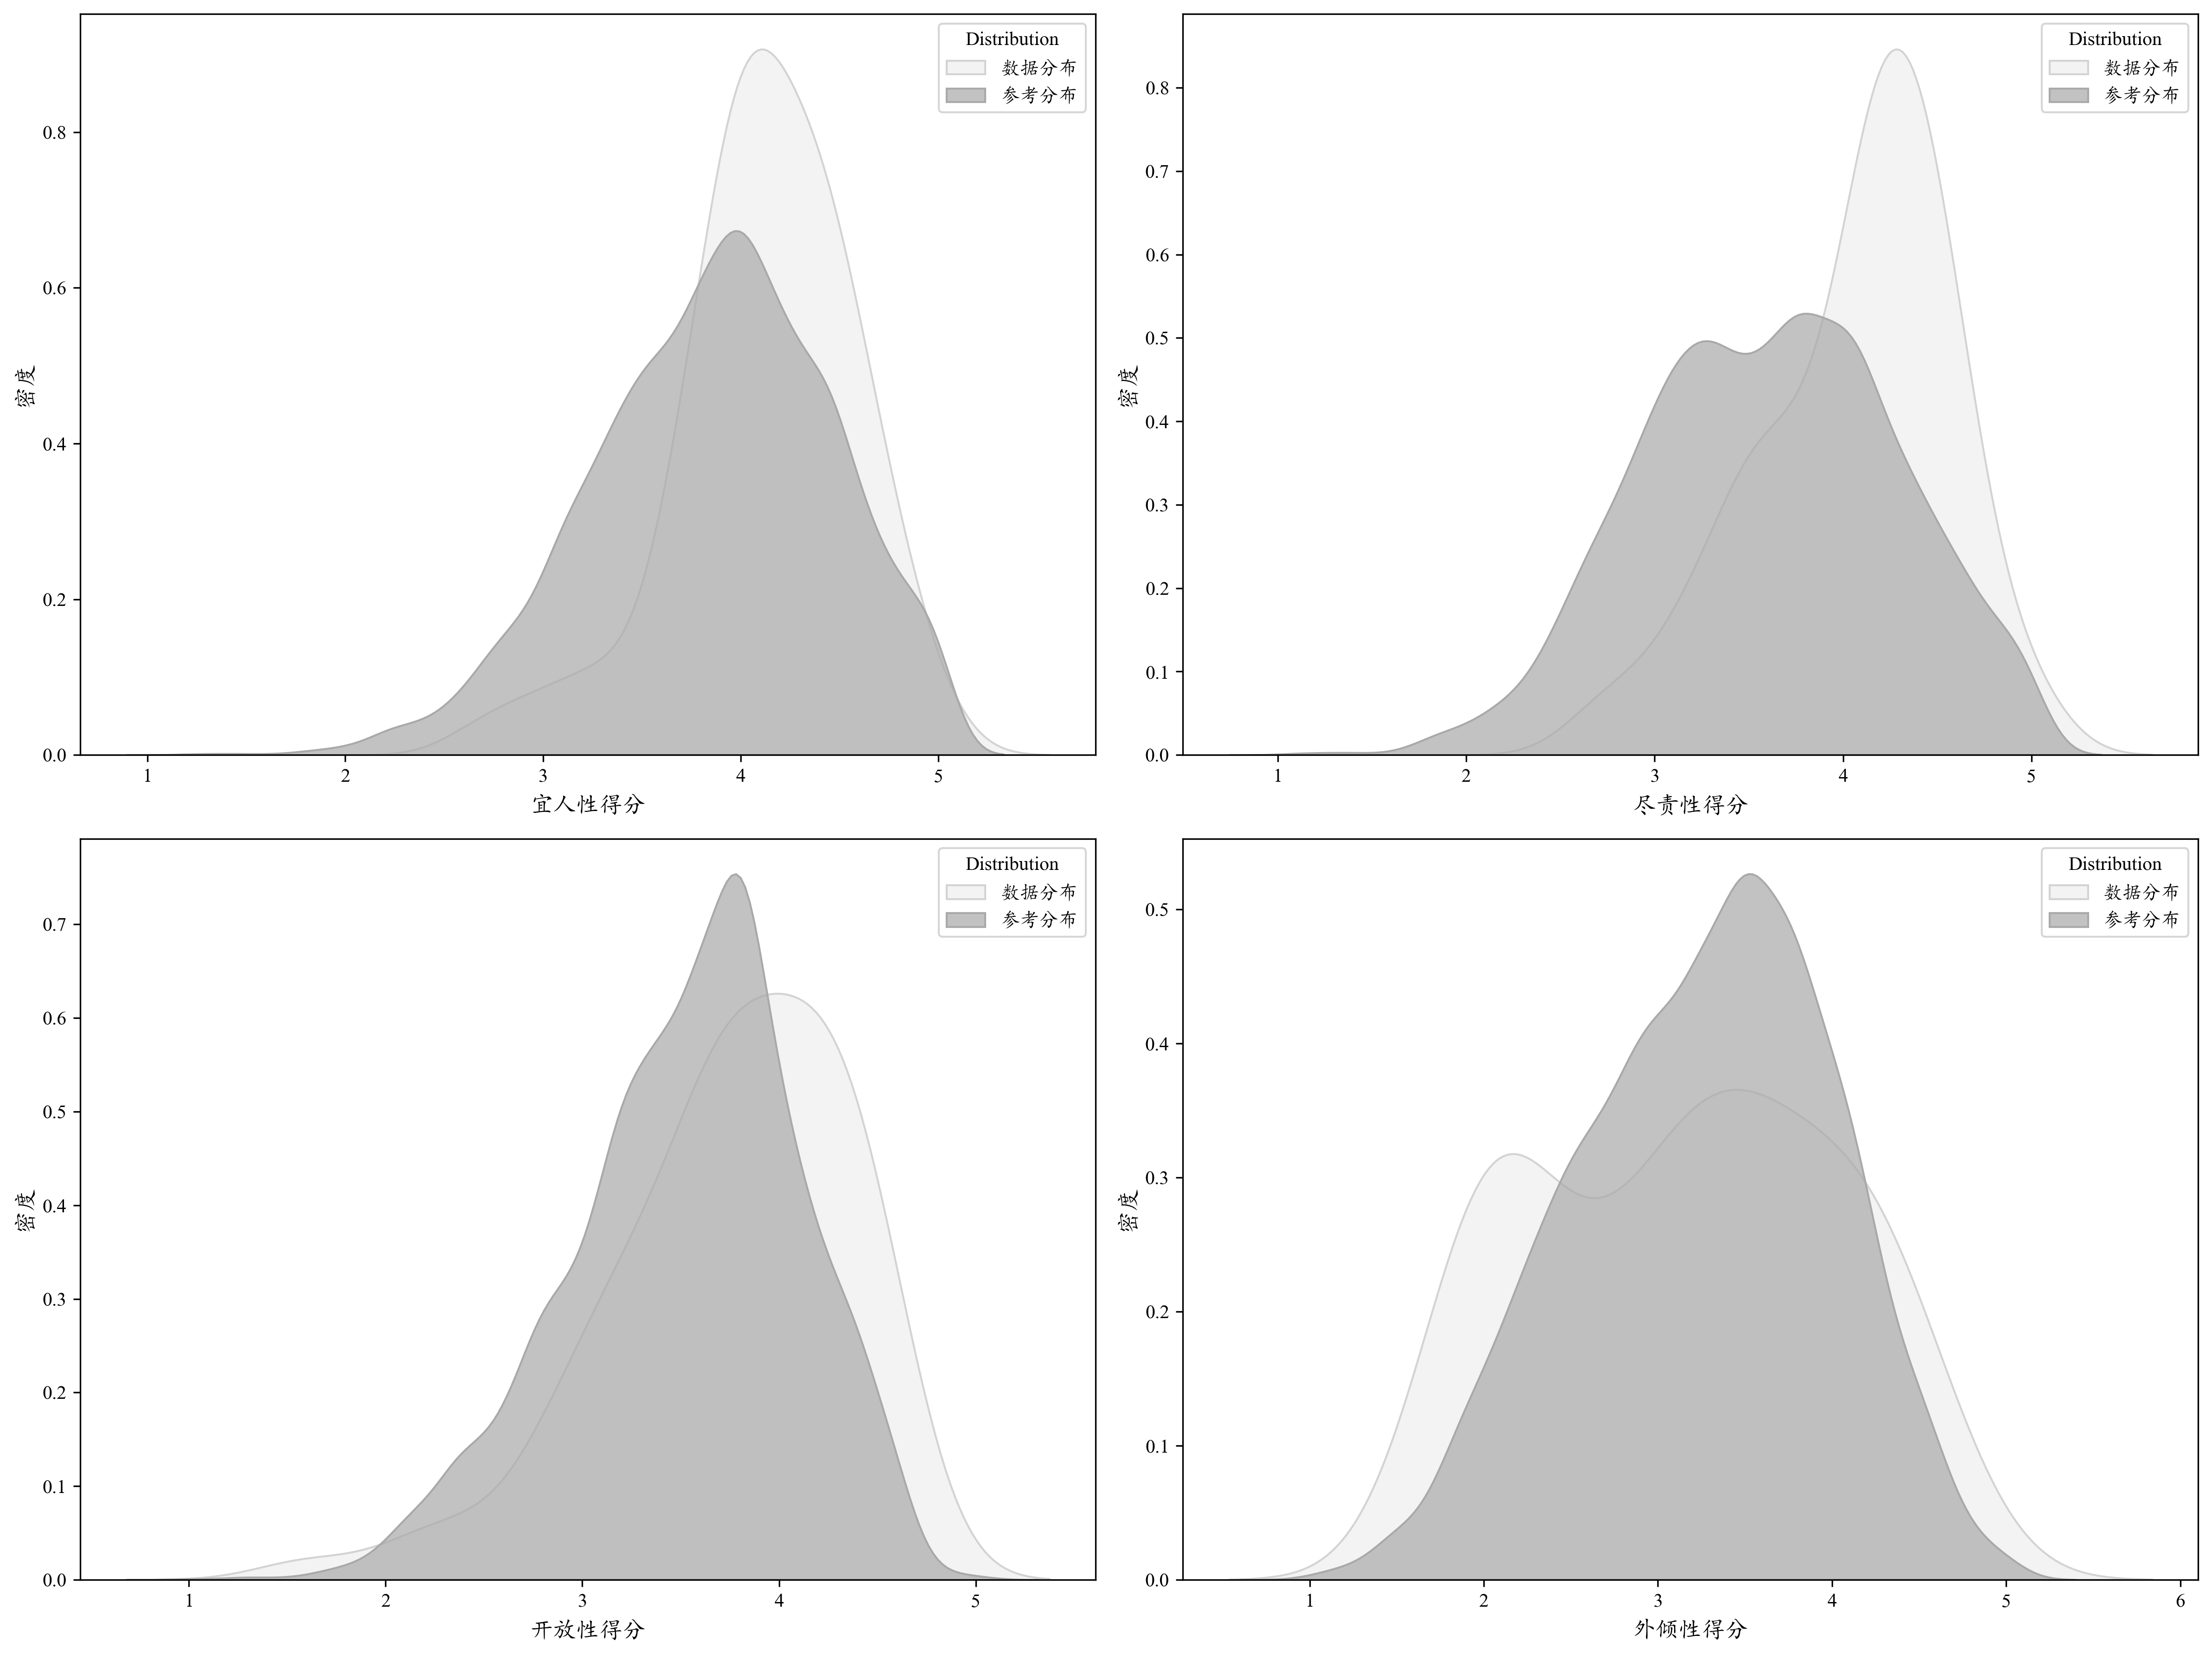
\includegraphics[width=1.0\linewidth]{Image/Study1-exp4-distribution.png}
    \caption{\label{fig:Study1-exp4-distribution}本研究与大样本数据(5110份)的人格特质分布比较}
\end{figure}


\section{讨论}
本研究通过四个实验系统性地探讨了AI基于大五人格特质生成个性化广告的能力,重点关注其在不同人格特质群体中的有效性,并考察了AI在不同广告创作情境下的适用性。研究结果提供了对 AI 生成广告个性化能力的初步验证。

首先\textbf{实验1}作为AI生成个性化广告的初步验证,采用GPT-3.5生成针对大五人格五个维度的个性化广告,结果显示针对\textit{高外倾性}和\textit{高宜人性}设计的个性化广告具有显著的说服效果,\textit{高开放性}呈边缘显著;而\textit{高尽责性}、\textit{高神经质}的广告效果并不显著。这表明AI在某些人格特质群体(如高宜人性和高外倾性)中能够有效生成个性化广告,而在其他人格特质(如高尽责性和高神经质)中,其个性化效果仍存在一定局限。在\textbf{实验2}中,我们进一步考察了AI在不同产品场景下的个性化广告生成能力,并采用GPT-4进行广告创作。实验结果表明,相较于实验1中的 GPT-3.5,GPT-4 能够更有效地生成针对高开放性和高尽责性个体的个性化广告,并在不同产品类型(享乐型 vs. 实用型)中展现出稳定的个性化广告生成能力。这一结果表明,AI 不仅可以基于大五人格进行个性化创作,还能够根据产品类型调整个性化策略,进一步增强广告的针对性和说服力。此外,该实验还验证了AI在基于中性广告进行个性化改写的能力,说明AI可以在已有广告文本的基础上进行个性化调整,而不仅仅是从零生成个性化广告。相较于实验1采用的 GPT-3.5,GPT-4在生成个性化广告方面表现出更强的能力,尤其在开放性和尽责性个体中,其个性化广告的说服力得到了显著提升。这一结果不仅说明 AI 生成的个性化广告效果在不同产品类别中具有一定的稳定性,也表明随着 AI 语言模型能力的提升,其个性化生成效果可能进一步优化。

虽然已有研究表明个性化广告的有效性,但大多数研究仍局限于针对各人格特质的高水平设计 \citep[如][]{hirsh2012personalized,matz2017psychological,winter2021effects}),而对低水平人格特质的个性化广告研究仍然有限,且缺乏系统性探讨。本研究的\textbf{实验3和实验4}进一步考察了AI在不同人格特质水平(高 vs. 低)下的个性化广告生成能力。\textbf{实验3} 结果表明,在\textit{开放性、外倾性和宜人性}维度上,AI生成的个性化广告能够有效匹配目标受众的个性特质,即高水平个体更偏好针对高水平特质设计的广告,低水平个体更偏好针对低水平特质设计的广告。然而,在尽责性维度上,并未观察到显著的匹配效应,这表明尽责性个体的广告偏好可能受其他因素影响,或现有个性化策略仍需进一步优化。此外,关键词分析结果进一步验证了个性化广告的有效性,发现高水平特质个体在广告中更关注符合自身人格特质的关键描述,而低水平特质个体则更倾向于与其匹配的词语特征。在\textbf{实验4}中,我们探讨了AI在基于产品描述直接生成个性化广告的能力,考察其在缺乏中性广告的情况下,是否能够生成符合不同人格特质的个性化广告。结果显示,在\textit{开放性和外倾性}维度上,AI生成的个性化广告仍然表现出显著的匹配效应,高水平特质个体更偏好高水平个性化广告,低水平特质个体则更偏好低水平个性化广告。然而,在\textit{尽责性}维度,个性化效果呈现负向匹配效应,即高尽责性个体更偏好针对低尽责性设计的广告,而低尽责性个体更偏好针对高尽责性设计的广告,这可能与尽责性个体的审慎决策模式有关。此外,在\textit{宜人性维度}上,并未观察到显著的个性化效果,可能是由于宜人性个体的广告偏好差异较小,或是由于实验样本在高宜人性个体中存在较大异质性,影响了个性化匹配的稳定性。这一结果提示,未来研究在优化个性化广告的生成策略时,应进一步考察不同人格特质群体在广告偏好上的具体特征,并结合精细化的提示语(prompt)优化AI生成的广告内容,以提高个性化效果的精准度。

综合来看,本研究对个性化广告的研究进行了补充和拓展。首先,\textbf{实验1和实验2} 说明了AI生成的个性化广告在\textbf{部分人格特质群体}中的有效性,这与\citet{hirsh2012personalized} 和\citet{matz2017psychological} 的结论一致,同时也为\citet{winter2021effects} 提出的个性化广告可能不总是有效的观点提供了新的解释。其次,通过\textbf{实验3和实验4} 的探讨,本研究进一步揭示了\textbf{个性化广告在不同人格水平群体中的匹配效应},并发现尽责性维度的负向匹配效应可能源于广告内容设计与目标群体需求的不匹配。此外,在已有的AI生成个性化广告研究(如\citet{matz2024potential})的基础上,本研究更系统地考察了\textbf{AI在多个生成场景(如基于中性广告改写、基于产品描述直接生成)的个性化能力},并引入了高低人格水平的实验设计,以更全面地检验AI生成个性化广告的有效性。

此外,无论是本研究的研究一,还是既有关于AI在说服性文本生成方面的研究 \citep[如][]{bai2023artificial,goldstein2024persuasive},均主要聚焦于AI本身的能力,而较少涉及AI在与人类专家的直接比较中的表现。然而,以往的说服性研究多基于人类专家或个体创作的文本,因此,将AI与人类专家进行对比不仅能够提供更精确的基准,以衡量AI在个性化广告创作中的实际水平,还能进一步揭示其在不同情境下的适用性与局限性。人类专家长期以来被视为广告创作的标准,其具备更丰富的市场洞察力、更复杂的创意表达方式以及更强的受众情感共鸣能力,而AI则凭借高效的文本生成能力和个性化调整优势,在广告创作中展现出潜在价值。因此,明确AI生成的个性化广告在说服效果上是否能够达到人类专家的水平,或者在人格化定制的特定场景下是否能够展现出特定优势,是一个值得深入探讨的问题。

此外,研究一的结果表明,AI在不同人格特质条件下的个性化广告生成能力并不均衡。例如,在尽责性和宜人性维度上的个性化效果未能稳定显现,甚至在尽责性维度上出现了负向匹配效应。这一现象进一步引发了对于个性化广告稳定性的讨论,即人类专家创作的广告是否能在不同人格特质条件下展现出更稳定的说服效果? 现有文献亦表明,AI的说服效能可能因任务性质和应用情境的不同而存在差异。例如,\citet{huang2023artificial} 研究发现,AI在塑造行为意图方面的效果低于人类专家,但在影响个体感知、态度和实际行为方面,与人类专家并无显著差异。因此,在个性化广告这一特定应用场景下,AI与人类专家在说服力上的比较仍然缺乏系统性的实证研究。AI是否能在广告个性化定制中与专家的创作水平相匹配?不同人格特质群体对于AI与专家创作的广告是否存在差异化的接受度?这些问题将在研究二中展开系统性探讨,以进一步评估AI在个性化广告中的优势与局限,并深化对AI生成广告在实际市场应用中的有效性及边界的理解。
% \section{子研究一:AI与人类专家在个性化广告创作中的表现}
\chapter{研究二:AI与专家在个性化广告中的效果比较}

现有研究已开始对AI与人类在说服性文本中的差异进行初步探索。\citet{bai2023artificial} 通过三项预注册实验(N=4,836)系统探讨了 GPT-3 在不同政策议题上的说服能力,并与人类的说服文本进行对比。结果显示,从说服效果角度而言,AI和人类创作的文本同样有效,但是从感知层面来说,两者的文本存在一定差异, AI生成的文本更加基于证据、逻辑性更强,而人类撰写的文本则更倾向于强调个人经验、叙事性表达和生动的意象。然而,该研究主要聚焦于 AI 在一般性说服任务中的能力,而在个性化广告领域,AI 相较于人类专家是否同样具有竞争力,仍然值得进一步探讨。传统的说服研究通常关注文本的逻辑性、事实性和情绪表达,而个性化广告不仅涉及说服性文本的质量,还需要精准匹配目标受众的人格特质。在这一背景下,AI可能具备一定优势,因其可以基于大规模数据训练,对人格特质的理解可能更为全面和丰富,并得益于生成能力,能据此生成针对性的广告内容。然而,个性化广告的核心在于感知匹配(perceived fit),即广告内容与目标受众的个性特质、偏好和需求之间的契合程度\citep{wheeler2005self}。相比一般的说服场景,个性化广告强调的是消费者的自我认同与个性表达,而不仅仅是基于理性信息的劝服。在这种情境下,个性化广告不仅需要传递逻辑清晰、基于证据的信息,还需要营造一种体验感,让受众能够在广告中看到自己、感受到品牌与自己的契合\citep{phillips1997thinking}。人类专家可能在这类广告创作中具备优势,因为他们能够利用叙事策略、社会文化背景和消费者心理,将广告塑造为更贴合个体认知和情感需求的体验。同时除了单一的人类专家和AI,越来越强调人际合作 \citep{karinshak2023working},即人机合作可能更能发挥两者的优势。

基于此,研究二将比较AI与人类专家生成的个性化广告效果。实验1主要聚焦于人类专家 vs. AI(GPT-4)的对比,以评估标准 AI 生成的个性化广告与专家创作的广告在说服力上的差异。而实验2进一步引入AI修改(GPT-loop),即AI基于人类专家生成的个性化广告进行进一步修改,以探讨AI和人类合作是否能否提升个性化广告效果,并使其达到或超越人类专家或者AI水平。通过这两个实验,研究二将系统检验AI在个性化广告创作中的适用性,并进一步揭示AI在说服性广告领域的优势和局限。

\section{实验1:AI与人类专家在不同人格特质广告生成中的比较} 

\label{实验1:GPT-4与人类专家在不同人格特质广告生成中的比较}

\subsection{方法}
本实验采用 \textbf{2(信息创作者:AI/人类专家)}的被试间设计。AI条件选取当前表现最优的模型GPT-4,人类专家以心理学专业研究生作为代表。广告通过针对五种不同人格水平(外倾性、开放性、尽责性、宜人性、神经质)的高水平特质进行个性化设计,即分别为高外倾、高开放、高尽责、高宜人和高神经质的消费者设计了广告内容。每类信息创作者(AI/人类专家)针对每种人格水平生成 3-5 则广告,每位被试被随机分配到一类信息创作者的广告条件,并从每个人格水平对应的 3 则广告中随机选择 1 则进行呈现。被试依次观看五则广告(对应五种人格水平),广告呈现顺序随机,且需对每则广告进行评价。

\textbf{(1)被试}

通过见数平台发布实验,366名参与者自愿参加这项研究。28名参与者由于注意检查测试未通过被剔除,剩余\textbf{322}名有效被试(年龄范围= 18-58岁;\textit{M}=29.43岁;\textit{SD}=7.36;女性203名)。参与任务的每名参与者获得5元人民币作为报酬。其中注意力检测题为一道见数平台自带的题目:“今天天气不错,请选2”,若未选2,则被判定为注意力检测题未通过。

\textbf{(2)问卷测量}

a. 大五人格量表。BFI10量表(详见同研究一实验1 \ref{study1-substudy1-measurement})。

b. 说服效果。具体的题项与实验1一致(详见 \ref{study1-substudy1-measurement},包含五个题项,用于评估参与者对广告和产品的态度以及购买意图。每个题项均采用1-5点李克特量表评分,广告说服效果的总评分为五个题项得分的平均值。

\textbf{(3)广告材料}

针对2(信息创作者:AI/人类专家)*5(广告人格:外倾性/开放性/尽责性/宜人性/神经质)共10个条件生成广告材料。AI条件选取当前表现最优的模型GPT,人类专家以心理学专业研究生作为代表。根据前人文献选择中性的产品手机,广告描述避免具体品牌名以排除品牌的影响。提供给GPT和人类专家的指导语是相同的,包括对目标消费者特点的描述(个性化,具体的人格描述参考人格特质量表中的描述)以及广告基本特征的描述。

每个条件生成5-6个信息,初始生成53则广告文本材料,经过预实验筛选,剩余38条(详见附录)。通过见数平台发布实验,140名参与者自愿参加预实验(年龄范围= 18-65岁;\textit{M}=32.26岁;\textit{SD}=10.05;女性69名)。每名参与者只看一个条件中的随机一则广告文本材料,条件之间的顺序随机。阅读完一则广告文本材料后,参与者需要选择这则广告面向的消费者特点,并对广告理解(消费者能够理解该信息是在宣传手机)/相关程度(该广告与手机这一产品的相关程度)进行1-5点量表的评价。对于消费者特点,参与者需要在五个目标人格特点描述中选择与广告最相符的特点,描述同样参考人格特质量表中对特质的描述。我们通过两个筛选条件来选择用于正式实验的实验材料: 1)广告人格是选择目标人格是最多的;2)理解程度和相关程度均大于3分。最终筛选得到每个条件3-5则广告文本材料,具体的实验材料详见附录。

\subsection{实验流程} 
在实验开始前,参与者被告知接下来他们将对五则社交媒体上的广告进行评价。所有广告文案的配图相同(见图\ref{fig:Study2-exp1-ad-example}),区别在于广告文案内容。参与者将依次阅读五则广告的文案,并在每阅读完一则文案后立即对其说服效果进行评分。完成所有五则广告文案的评价后,参与者需回答与人格测试相关的问卷题目,最后提供年龄、性别等人口统计学信息。

\begin{figure}[htbp]
    \centering
    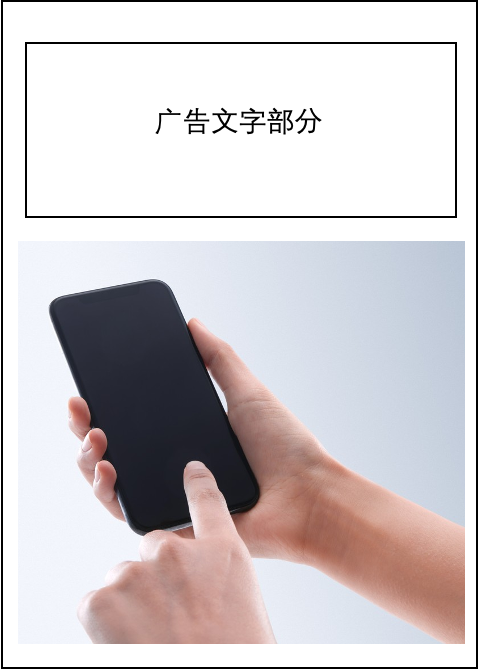
\includegraphics[width=.3\linewidth]{Image/Study2-exp1.png}
    \caption{\label{fig:Study2-exp1-ad-example}实验开始前的广告示意图}
\end{figure}

\subsection{结果}
首先分别对不同创作者(人类专家/GPT-4)生成的个性化广告效果进行检验。个性化效果通过建立人格水平与说服效果之间的线性回归模型来进行衡量,其中人格水平作为自变量,说服效果作为因变量。由于在本研究中,个性化广告是针对各人格维度的高水平个体进行设计的,因此理论上,当参与者在某一人格维度的得分越高时,相应该维度的个性化广告的说服效果越好。回归结果如下表所示(表 \ref{tab:study1_traitResults})。

结果表明,在GPT-4生成的广告中,宜人性(\textit{$\beta$} = 0.3765, \textit{p} = 0.002)、外倾性(\textit{$\beta$} = 0.1967, \textit{p} < 0.001)、尽责性(\textit{$\beta$} = 0.2978, \textit{p} < 0.001)、开放性(\textit{$\beta$} = 0.2808, \textit{p} = 0.001)四个维度上表现出人格水平对说服效果的显著正向预测效果,即宜人性/外倾性/尽责性/开放性水平越高的参与者,针对各维度高水平设计的广告说服效果更好。而神经质表现出显著相反的趋势(\textit{$\beta$} = -0.2479, \textit{p} < 0.001),即神经质水平越低越喜欢针对高神经质设计的广告。

在人类专家生成的广告中,仅宜人性(\textit{$\beta$} = 0.2685, \textit{p} = 0.004)和开放性(\textit{$\beta$} = 0.2399, \textit{p} = 0.016) 两个维度上表现出人格水平对说服效果的显著正向预测效果,即宜人性/开放性水平越高的参与者,针对各维度高水平设计的广告说服效果更好。外倾性维度上正向预测效果达到边缘显著水平(\textit{$\beta$} = 0.1343, \textit{p} = 0.087),尽责性人格水平呈正向预测效果但不显著(\textit{$\beta$} = 0.0932, \textit{p} = 0.229),而神经质人格水平的预测效果呈负向但不显著(\textit{$\beta$} = -0.1176, \textit{p} = 0.12)。

为进一步探讨人类专家与GPT-4在个性化广告创作水平上的差异,本研究对两类创作者回归斜率的差异进行了显著性检验。结果表明仅在尽责性维度上,人类专家与GPT-4的个性化水平之间差异达到边缘显著水平(\textit{t}(318) = 1.8128, \textit{p} = 0.07),具体而言,GPT-4生成的广告在该维度表现出显著的个性化效果,而人类专家的个性化效果不显著;在外倾性维度上,尽管两类信息创作者表现出不一样的趋势,即GPT-4的个性化水平显著,但人类专家的个性化水平边缘显著,但两者之间的斜率差异未达到显著水平(\textit{t}(318) = 0.6486, \textit{p} = 0.52);在宜人性(\textit{t}(318) = 0.7245, \textit{p} = 0.47)和开放性(\textit{t}(318) = 0.3115, \textit{p} = 0.76)维度上,GPT-4和人类专家在生成的个性化广告效果均显著,但两者之间不存在显著差异;在神经质维度,尽管两者存在一定的差异,但仍未达到显著水平(\textit{t}(318) = 1.4269, \textit{p} = 0.15)。

\FloatBarrier % 防止表格与正文之间的分离,强制插入位置

% \begin{table}[H]
%     \centering
%     \caption{\label{tab:study1_traitResults} 人格特质回归分析结果}
%     {\tablesongti % 整个表格环境应用宋体六号字体
%     \renewcommand{\arraystretch}{1} % 调整行距
%     \begin{tabularx}{\linewidth}{>{\raggedright\arraybackslash}X X c c c c c c}
%         \toprule
%         个性化特质 & 信息创作者 & 系数 & 标准误差 & \textit{t} & \textit{P} $>|t|$ & [0.025 & 0.975] \\ 
%         \midrule
%         \textbf{宜人性}   & \textbf{人类专家}  & 0.2685 & 0.0930 & 2.8860\textsuperscript{**} & 0.004   & 0.0848 & 0.4522 \\
%         \textbf{宜人性}   & \textbf{GPT-4}   & 0.3765 & 0.1166 & 3.2296\textsuperscript{**} & 0.002   & 0.1463 & 0.6068 \\
%         外倾性    & 人类专家   & 0.1343 & 0.0781 & 1.7206\textsuperscript{\dag} & 0.087   & -0.0198 & 0.2884 \\
%         \textbf{外倾性}    & \textbf{GPT-4}     & 0.1967 & 0.0562 & 3.5003\textsuperscript{***} & <0.001  & 0.0857 & 0.3077 \\
%         神经质     & 人类专家      & -0.1176 & 0.0752 & -1.5647 & 0.120   & -0.2661 & 0.0308 \\
%         \textbf{神经质}     & \textbf{GPT-4} & -0.2479 & 0.0518 & -4.7842\textsuperscript{***} & <0.001  & -0.3502 & -0.1455 \\
%         尽责性 & 人类专家  & 0.0932 & 0.0771 & 1.2080 & 0.229   & -0.0591 & 0.2455 \\
%         \textbf{尽责性} & \textbf{GPT-4}  & 0.2978 & 0.0825 & 3.6116\textsuperscript{***} & <0.001  & 0.1350 & 0.4607 \\
%         \textbf{开放性}        & \textbf{人类专家}        & 0.2399 & 0.0987 & 2.4309\textsuperscript{*} & 0.016   & 0.0450 & 0.4348 \\
%         \textbf{开放性}        & \textbf{GPT-4}         & 0.2808 & 0.0866 & 3.2407\textsuperscript{**} & 0.001   & 0.1097 & 0.4519 \\
%         \bottomrule
%     \end{tabularx}
%     }
%     % \vspace{1mm}
%     \caption*{\raggedright \footnotesize 注:*** $p < 0.001$,** $p < 0.01$,* $p < 0.05$,\textsuperscript{\dag} $p < 0.1$。}
% \end{table}

\begin{table}[H]
    \centering
    \caption{\label{tab:slope_difference} 不同创作者的回归斜率差异}
    {\tablesongti
    \renewcommand{\arraystretch}{1.2} % 调整行距
    \begin{tabularx}{\linewidth}{>{\centering\arraybackslash}p{3cm} >{\centering\arraybackslash}p{4cm} >{\centering\arraybackslash}p{4cm} >{\centering\arraybackslash}p{4cm}} % 居中对齐
        \toprule
        \textbf{特质} & \textbf{人类专家 (系数 \& }\textit{p}\textbf{ 值)} & \textbf{GPT-4 (系数 \& }\textit{p}\textbf{ 值)} & \textit{t 值 \& p 值} \\ 
        \midrule
        \textbf{宜人性}   & 0.2685 (0.004**)  & 0.3765 (0.002**)  & -0.7245 (0.47) \\
        \textbf{外倾性}   & 0.1343 (0.087\textsuperscript{\dag})  & 0.1967 (<0.001***)  & -0.6486 (0.52) \\
        \textbf{神经质}   & -0.1176 (0.120)  & -0.2479 (<0.001***)  & 1.4269 (0.15) \\
        \textbf{尽责性}   & 0.0932 (0.229)  & 0.2978 (<0.001***)  & -1.8128 (0.07\textsuperscript{\dag}) \\
        \textbf{开放性}   & 0.2399 (0.016*)  & 0.2808 (0.001**)  & -0.3115 (0.76) \\
        \bottomrule
    \end{tabularx}
    }
    \caption*{\raggedright \footnotesize 注:*** \textit{p} < 0.001,** \textit{p} < 0.01,* \textit{p} < 0.05,\textsuperscript{\dag} \textit{p} < 0.1。}
\end{table}






\section{实验2:引入AI修改专家内容的个性化广告效果}
实验1主要检验了GPT-4独立生成的针对大五人格高水平个体的个性化广告文案的效果,并与人类专家生成文案进行了比较。这一实验对AI生成个性化广告的潜在优势和局限性进行了初步评估。然而,实验1的研究设计在以下方面仍存在改进空间:

(1)人格测量工具的选择:实验1采用了BFI-10量表对参与者的人格特质进行测量,尽管简洁高效,但量表维度较短可能影响测量的精确性与信度。本实验改用BFI-44量表,以提升测量的标准化与可靠性,从而更全面地捕捉参与者的人格特质。

(2)因变量的设置:实验1的测量指标主要集中在广告的说服效果上,而忽略了广告在实际社交媒体场景中的潜在影响。为弥补这一不足,本实验在设计中新增了更加贴近实际应用的因变量,包括「支付金额」和「微博交互行为意愿程度」,以更全面地评估个性化广告的效果。

(3)人机协作情境的考察:实验1仅比较了GPT-4独立生成文案与人类专家生成文案的效果,未涉及AI与人类专家合作的情境。然而,在实际广告创作中,人机协作是AI技术应用的重要方向。为探讨GPT在辅助人类专家优化广告文案中的潜力,本实验新增了GPT对人类专家生成文案的修改组(即GPT-loop),以进一步评估GPT在协作场景下对广告文案效果的影响。

\subsection{方法}
根据上述调整,本实验采用 \textbf{3(信息创作者:AI/人类专家/AI修改专家)}的被试间设计。AI和人类专家条件与实验1保持一致 \ref{实验1:GPT-4与人类专家在不同人格特质广告生成中的比较},AI修改专家组为新增条件,在专家生成的文本基础上,引导AI对文案进行优化和调整。个性化条件与实验1一致,针对五种不同人格水平(外倾性、开放性、尽责性、宜人性、神经质)的高水平特质进行个性化设计,即分别为高外倾、高开放、高尽责、高宜人和高神经质的消费者设计了广告内容。

\textbf{(1)被试}

通过见数平台发布实验,378名参与者自愿参加这项研究。10名参与者由于注意检查测试未通过被剔除,剩余\textbf{368}名有效被试(年龄范围= 18-56岁;\textit{M}=25.70岁;\textit{SD}=6.63;女性228名)。参与任务的每名参与者获得5元人民币作为报酬。注意力检测题设置为人格测试中的一致性验证题,采用BFI-44量表中的原题和逆向表述的对比形式。具体而言,将BFI-44量表中的原题“我是健谈的”设置为其反向表述形式“我不是健谈的”。若参与者在这两道题目上的评分一致,且均不为中间分值(即3分),则被视为通过检测;否则,视为注意力检测未通过。


\textbf{(2)问卷测量}

a. 大五人格量表。采用\citet{john1991big}编制44道题目的大五人格量表(Big Five Inventory,BFI-44)测量参与者的人格特征。该量表共44个项目,分属外倾性、宜人性、神经质、开放性、尽责性5个维度。参与者在 5 点李克特式量表上进行评分(选项“1”代表“非常不符合”,“5”代表“非常符合”)。

b. 因变量。本实验设置三个因变量,分别为说服效果、微博互动意愿、支付金额。其中说服效果与实验1一致,具体测量方式详见表\ref{tab:persuasionSurvey})。微博互动意愿参考\citet{winter2021effects}的设计,通过四个题项评估参与者对广告微博可能产生的具体互动行为意愿。具体题目包括:(1)“我会点击并访问广告发布者的微博主页”;(2)“我会点赞该微博”;(3)“我会评论该微博”;(4)“我会转发/分享该微博”。参与者需基于五点李克特量表进行评分,其中“1”代表“非常低”,“5”代表“非常高”。支付金额参考\citet{matz2024potential}的方法,要求参与者对愿意为广告中的产品支付的金额进行评估,支付金额范围设置为0元至10000元人民币,具体金额区间是根据Canalys 2023年第二季度中国智能手机均价(约450美元,折合人民币3300元)合理扩展而来,旨在模拟实际消费场景。

\textbf{(3)广告材料}

针对3(信息创作者:AI/人类专家/AI修改专家)*5(广告人格:外倾性/开放性/尽责性/宜人性/神经质)共15个条件生成广告材料。广告内容的产品仍为手机,与实验1保持一致。

人类专家组的材料与实验1一致。在AI组和AI修改专家组中,广告文案则重新生成。尽管AI组在实验1中已存在,但为确保本实验中AI相关条件的一致性,AI组与AI修改专家组的文案均由相同的模型生成。在AI修改专家组中,文案生成的具体操作是基于专家组的原始文案进行改写,明确要求GPT以专家文案为基础对内容进行优化调整,而非直接生成全新的文案。每个条件生成5-6个信息,初始生成53则广告文本材料,经过预实验筛选,剩余38条(详见附录)。通过见数平台发布实验,329名参与者自愿参加预实验(年龄范围= 18-72岁;\textit{M}=30.44岁;\textit{SD}=9.35;女性200名)。每名参与者仅参与一个实验条件,即针对某一信息创作者生成的广告文案和某一人格维度设计的广告材料进行评价。每个条件下包含5-6则广告文案。参与者在阅读每则广告文案后,需根据广告面向的目标消费者特点进行评价。评分采用1-5点量表,其中1分表示更符合“低水平”描述,5分表示更符合“高水平”描述。例如,对于针对高尽责性设计的广告,参与者需基于以下特征进行评分,从“粗心的、容易分心的、不拘小节的、做事缺少条理的”到“可靠的、有组织的、自律的、注重细节的、有条理”。此外,参与者还需对广告的理解程度(即消费者是否能理解广告是在宣传手机)进行1-5点量表评分。预实验通过两个筛选条件来选择用于正式实验的实验材料: 1)广告目标消费者特点评分需大于3分;2)广告理解程度评分需大于3分。根据以上筛选标准,最终保留每个条件下2-6则广告文本材料用于正式实验,具体材料详见附录。

\subsection{实验流程}
在实验开始前,参与者被告知接下来他们将对五则社交媒体上的广告进行评价。所有广告文案的配图相同(见图\ref{fig:Study2-exp2-ad-example}),区别在于广告文案内容。为了模拟更实际的社交媒体场景,相较于实验1,本实验的广告界面增加了微博平台的视觉元素,包括虚拟的头像、虚拟的微博账号名,以及点赞、评论和转发等交互按键。参与者将依次阅读五则广告的文案,并在每阅读完一则文案后立即对其说服效果/微博参与意愿/支付金额进行评分。完成所有五则广告文案的评价后,参与者需回答与人格测试相关的问卷题目,最后提供年龄、性别等人口统计学信息。

\begin{figure}[htbp]
    \centering
    
\includegraphics[width=.3\linewidth]{Image/Study2-exp2.png}
    \caption{\label{fig:Study2-exp2-ad-example}实验开始前的广告示意图}
\end{figure}


\subsection{结果}
本实验的分析方法与实验1相似,分别对不同信息创作者(人类专家/AI/AI修改专家)生成的个性化广告效果进行检验。个性化效果通过建立人格水平与因变量(说服效果、微博互动意愿、支付金额)之间的线性回归模型来衡量,其中人格水平作为自变量,三个效果指标作为因变量。由于在本实验中,个性化广告是针对各人格维度的高水平个体进行设计的,因此理论上,当参与者在某一人格维度的得分越高时,相应维度的个性化广告的效果指标应表现更好。此外,由于支付金额的范围较广(0-10000元),在分析过程中对其进行了归一化处理。

结果表明,在三个广告效果指标上,AI (GPT-4) 和 AI 修改专家组 (GPT-4 修改专家) 在宜人性、外倾性、尽责性和开放性四个维度上均表现出稳定且显著的个性化效果(回归显著,\textit{p}s < 0.05)。这说明,特质得分越高,针对高特质设计的广告效果越好,符合预期。而在神经质维度上,三个创作者的广告均表现出稳定的负向结果,即神经质得分越低,针对高神经质设计的广告效果评价越高。人类专家组在外倾性、尽责性和开放性维度上也表现出显著的个性化效果,且与 AI 组和 AI 修改专家组结果一致。但在人类专家组中,宜人性维度的个性化效果不显著(\textit{p} > 0.05)。

\begin{table}[H]
    \centering
    \caption{\label{tab:slope_difference_study2} 不同创作者的回归斜率差异(说服效果)}
    {\tablesongti
    \renewcommand{\arraystretch}{1.2} % 调整行距
    \begin{tabularx}{\linewidth}{>{\centering\arraybackslash}p{3cm} >{\centering\arraybackslash}p{4cm} >{\centering\arraybackslash}p{4cm} >{\centering\arraybackslash}p{4cm}} % 居中对齐
        \toprule
        \textbf{特质} & \textbf{人类专家 (系数 \& }\textit{p}\textbf{ 值)} & \textbf{GPT-4 (系数 \& }\textit{p}\textbf{ 值)} & \textbf{GPT-Loop (系数 \& }\textit{p}\textbf{ 值)} \\ 
        \midrule
        \textbf{外倾性}   & 0.3145 (0.002**)  & 0.3143 (0.001**)  & 0.3431 (0.001**)  \\
        \textbf{宜人性}   & 0.1270 (0.419)  & 0.4350 (0.003**)  & 0.6969 (<0.001***)  \\
        \textbf{尽责性}   & 0.3221 (0.002**)  & 0.4375 (<0.001***)  & 0.4022 (0.001**)  \\
        \textbf{神经质}   & -0.3358 (0.001**)  & -0.3423 (0.001**)  & -0.4036 (0.001**)  \\
        \textbf{开放性}   & 0.4017 (0.004**)  & 0.4859 (<0.001***)  & 0.6110 (<0.001***)  \\
        \bottomrule
    \end{tabularx}
    }
    \caption*{\raggedright \footnotesize 注:*** \textit{p} < 0.001,** \textit{p} < 0.01,* \textit{p} < 0.05,\textsuperscript{\dag} \textit{p} < 0.1。}
\end{table}


进一步,我们比较了三类信息创作者在回归斜率上的显著性差异。结果表明,仅在宜人性维度上,AI 修改专家组与人类专家组在说服效果(\textit{t} = 2.66,\textit{p} = 0.008)和微博互动意愿(\textit{t} = 1.96,\textit{p} = 0.05)两个指标上表现出显著差异。人类专家组本身的个性化效果不显著,而 AI 和 AI 修改专家组的个性化效果显著且稳定。同时,显著性差异检验表明 AI 修改专家组显著优于人类专家组。这一结果说明,GPT-4 在优化人类专家文案时能够显著提升宜人性维度广告的效果。此外,与实验1相比,人类专家组在宜人性维度上的表现发生了变化:实验1中,人类专家组的宜人性个性化效果显著,而本实验中则未达到显著性水平。为探讨这一差异,本研究分析了实验1和本实验所使用的人格测量工具(BFI-10 和 BFI-44)的相关性(如图\ref{fig:study2-correlation})。结果显示,宜人性维度的相关性较低(0.67),而其他四个维度的相关性均较高(>0.80)。这表明,本实验中使用的 BFI-44 测量工具具有更高的精确度和可靠性,因此本实验的结果更可信。此外,在实验1中,人类专家组在外倾性和尽责性维度上未表现出显著的个性化效果,但在本实验中,这两个维度的效果变得更显著。结合测量工具的改进,可以推测,使用更精细的量表后,外倾性和尽责性维度的个性化效果更加稳定。

\begin{figure}[H]
    \centering
    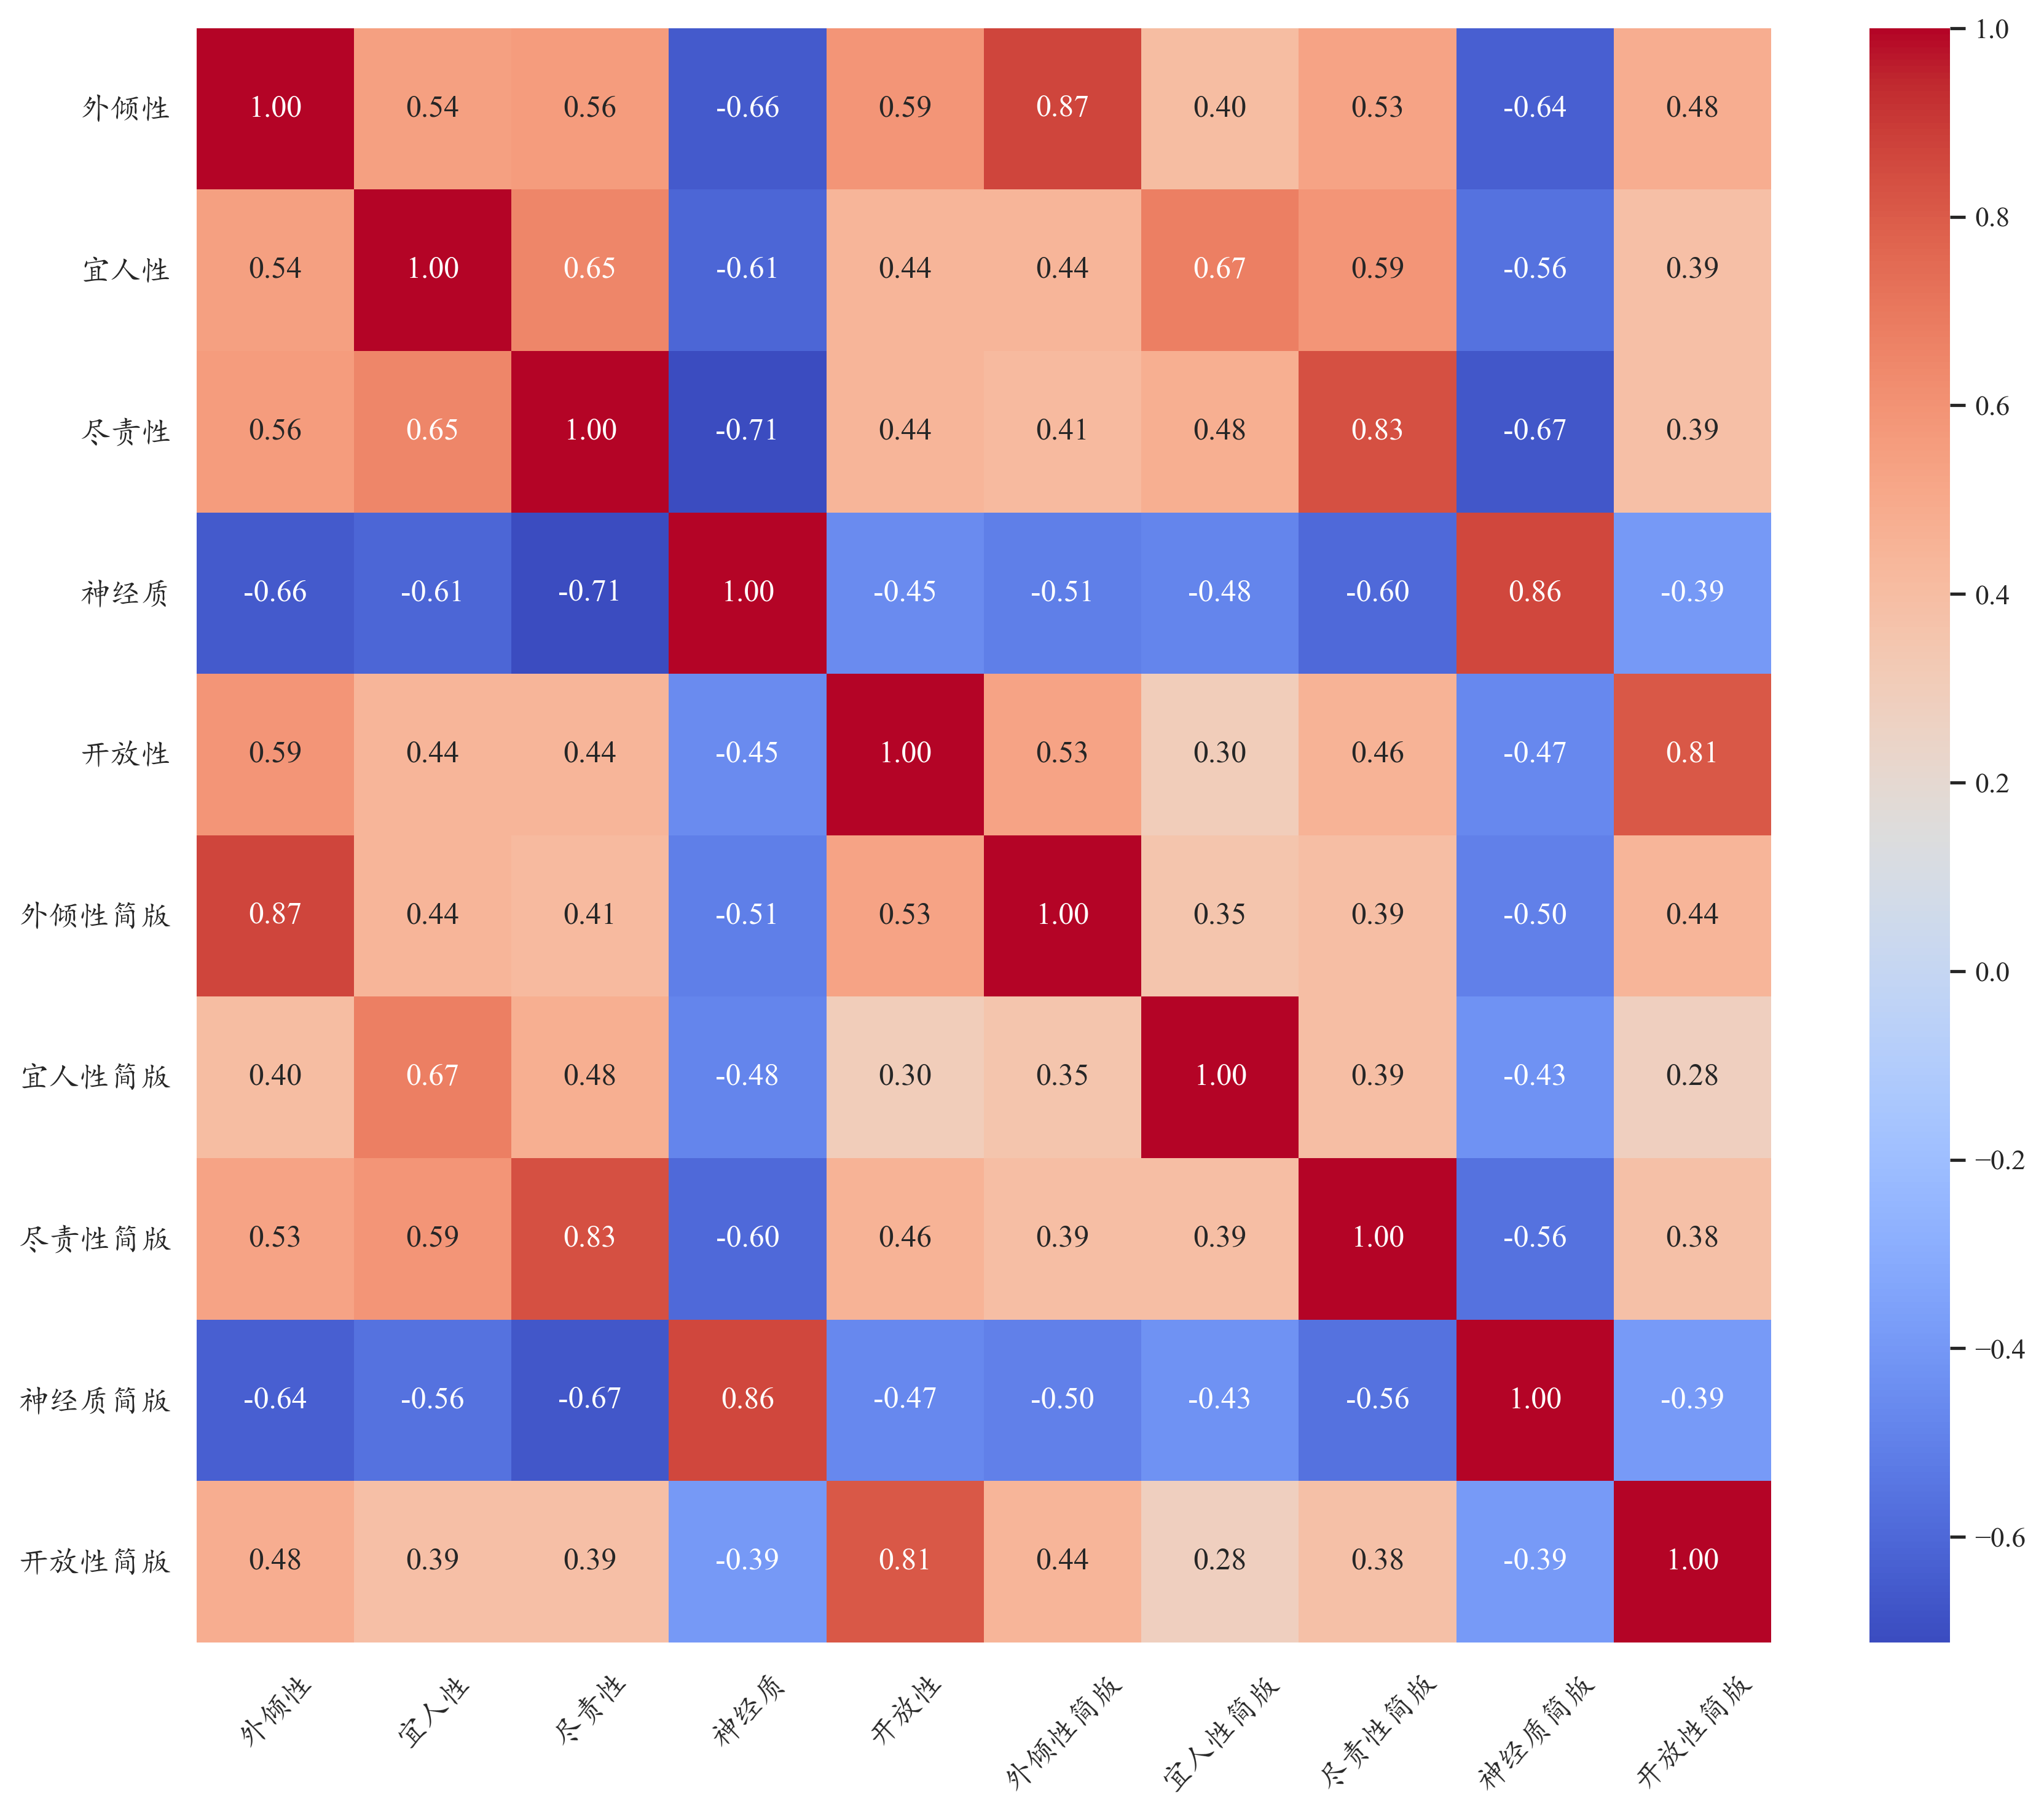
\includegraphics[width=1\linewidth]{Image/BFI44-BFI10相关.png}
    \caption{\label{fig:study2-correlation}BFI44-BFI10相关}
\end{figure}

神经质维度的负向结果表现出一致性。以说服效果为例,AI组(\textit{$\beta$} = -3.410, \textit{p} < 0.01),人类专家组(\textit{$\beta$} = -3.441, \textit{p} < 0.01),AI修改专家组(\textit{$\beta$} = -3.571, \textit{p} < 0.01)在神经质维度上均呈现显著负向预测趋势,即神经质得分较低的个体对针对高神经质设计的广告评价更高。这一结果与前人研究中提到神经质的特殊性一致\citep{matz2024potential}。这一现象的机制可能与高神经质广告传递的情感特征有关,后续研究将进一步结合对 AI 生成广告特征的内容分析进行深入探讨。

综上所述,本实验的结果表明,AI 和 AI 修改专家组在宜人性、外倾性、尽责性和开放性维度上均表现出显著且稳定的个性化效果,而人类专家组在宜人性维度上的表现不如预期,但在外倾性、尽责性和开放性维度上仍显示出一定能力。特别是AI修改专家组在宜人性维度上的显著提升,进一步证明 AI 技术不仅能够独立生成高效的个性化广告,还可以通过与人类专家协作进一步优化广告内容,从而为个性化广告设计中的人机协作提供重要启示。





\section{讨论}

本研究通过实验1和实验2系统地比较了AI(GPT-4)与人类专家在个性化广告创作中的表现,并进一步探讨了AI优化人类专家广告文案的潜力。结果表明,AI能够在多个人格特质维度上生成有效的个性化广告,且在某些特质(如尽责性)上,其个性化效果甚至优于人类专家。此外,当AI用于优化人类专家文案时,个性化广告的效果在宜人性维度得到了显著提升。这一发现不仅为AI在个性化广告领域的应用提供了新的证据,也为更广泛的说服与信息传播研究提供了重要启示 \citep{dehnert2022persuasion}。

尽责性和宜人性两个特质的个性化广告在实验结果中展现出了一定的复杂性。在尽责性维度上,GPT-4 生成的广告表现出稳定的个性化匹配效果,而人类专家的个性化效果则不显著,且GPT-4和人类专家的效果在实验1中存在边缘显著的差异。这一结果表明,AI在尽责性个性化广告的创作上具有更强的适配性,而人类专家在这一维度的广告效果则存在较大的不确定性。尽责性人格的核心特征包括自律、责任感和条理性\citep{roberts2014conscientiousness},这类个体通常偏好结构清晰、信息明确、逻辑严谨的广告内容。然而,人类专家在撰写广告时可能受到自身写作风格的影响,使得广告文本在逻辑性和条理性上存在个体差异,导致尽责性个性化广告的效果不稳定。而GPT-4 作为基于大规模语料训练的AI模型,能够在生成过程中更一致地遵循逻辑清晰、信息直接的模式,因此其尽责性个性化广告更具稳定性。这也说明,通过优化prompt以及随着模型能力的提升,AI在尽责性个性化广告创作中的适应性可能仍在增强。

在宜人性维度上,实验2的结果显示,GPT-4 修改人类专家文案后,其个性化广告在说服效果和微博互动意愿方面均显著优于人类专家组,而人类专家组本身的个性化效果未达到显著水平。这一发现表明,在宜人性个性化广告的创作过程中,AI不仅能够独立生成有效的个性化广告,还能够优化人类专家的广告,使其更符合目标受众的需求。宜人性人格的个体通常更加注重社交互动、合作与温暖的表达\citep{graziano2007agreeableness},这意味着个性化广告需要更强的情感共鸣和人际取向。然而,人类专家可能并未能充分把握宜人性个体的偏好,导致其广告在实验间表现出较大的不稳定性。而AI在优化人类专家广告时,能够更系统性地强化广告中的情感元素和亲和力表达,使其更符合高宜人性个体的预期。这表明,在个性化广告创作中,AI不仅能够弥补人类专家可能存在的个性化表达不足,还能够通过文本优化进一步提升广告的个性化适配度。

另一方面,在神经质维度上,实验1和实验2均未能发现预期的个性化效果,且在实验2中,所有创作者的广告均表现出稳定的负向匹配效应,即神经质水平较低的个体对针对高神经质设计的广告评价更高。这一现象可能表明,神经质个体在广告偏好上的特征较为特殊,并不容易通过传统的个性化匹配策略进行有效优化。一个可能的解释是,高神经质个体通常具有较高的焦虑和不安全感,因此他们可能更倾向于接受带有安抚性、稳定性描述的广告,而不是直接迎合其负面情绪特征的广告。而低神经质个体可能对“高神经质广告”中涉及的情绪化表达、焦虑驱动的语言特征更敏感,甚至产生更强的情绪共鸣,从而导致负向匹配效应的出现。此外,高神经质个体可能对广告信息的解读方式不同于低神经质个体,他们更容易受到信息的情绪基调和潜在风险暗示的影响这可能进一步导致高神经质个体对高神经质广告的接受度较低,而低神经质个体则因广告的情绪化特征反而产生更高的评价。这一发现提示,在未来的个性化广告优化中,需要更深入地探讨神经质个体对广告内容的具体偏好模式,以避免简单的人格匹配策略在这一特质上的局限性。

尽管研究一和研究二验证了AI在个性化广告创作中的有效性,并探索了其与人类专家在个性化匹配效果上的差异,但这些实验的分析主要基于参与者被试的行为反馈,而未能深入解析广告文本本身的特征。特别是在尽责性和宜人性维度,AI展现出更稳定且更优的个性化匹配能力,而人类专家创作的广告则表现出较大的不确定性,这一结果表明,个性化广告的效果不仅受到受众人格特质的影响,也可能取决于广告文本本身的语言模式。然而,目前的实验结果仍未能清楚地揭示个性化广告创作中所采用的文本特征究竟存在何种系统性的差异,以及这些文本特征如何影响受众对广告的接受度。因此,仅通过参与者评分来判断个性化广告的有效性仍然是不够的,进一步的文本分析有助于揭示广告文本本身的结构、内容以及语言特征如何与不同人格特质的受众需求相匹配。在个性化广告研究中,文本特征的作用往往难以被系统地研究,因为传统的广告文本数量较少,难以进行规模化的文本分析。然而,AI的快速生成能力使得本研究能够积累大量的个性化广告文本及其参与者评分数据,从而为文本特征的深入分析提供了可能性。研究三将在研究一和研究二的基础上,结合大规模文本数据,系统地分析个性化广告文本在不同人格特质维度上的语言模式,并构建预测模型,以识别最能影响个性化广告说服效果的关键特征。这不仅能够帮助我们更好地理解AI在个性化广告创作中的优势与局限,也能为未来的人机协作广告创作提供数据驱动的优化策略,从而推动个性化广告生成技术的进一步发展。



% ----------研究三
\chapter{研究三:基于文本特征与用户偏好的个性化广告效果模型构建}

相关研究表明,人格特质与语言表达模式之间存在密切关系,但这些研究成果主要来源于社交媒体等用户生成内容 (User-Generated Content, UGC) 领域 \citep{azucar2018predicting}。例如,有研究发现,高外向性个体在社交媒体中的语言风格通常更为积极且富有互动性,而高开放性个体则偏好多样、富有创造性的语言表达。此外,通过分析用户在社交媒体中的点赞、评论和转发行为,研究者能够有效预测用户的大五人格特质。这些研究不仅证实了人格特质与语言特征之间的紧密联系,也展示了语言风格在反映个体心理特质中的重要作用。然而,这种“人格-语言”关联是否同样体现在基于人格定制生成的广告文案中,仍然缺乏系统性验证。与社交媒体中的自然语言表达不同,广告文本具有传播目的明确、语言风格结构化等特点,其语言特征是否能够如社交媒体内容般准确反映目标人格特质,尚不明确。造成这一研究空白的重要原因在于传统实验中的广告样本数量有限,难以支撑大规模、多维度的人格-语言特征系统分析。以往研究往往依赖人类专家创作广告文本,样本规模小且创作风格易受主观偏好影响,难以全面揭示不同人格设定下广告语言特征的差异性。然而,随着生成式人工智能 (Generative AI, 如 GPT) 技术的快速发展,研究者得以突破这一限制。AI能够批量生成符合不同人格设定的大规模广告文本样本,并在生成过程中严格控制语言风格以匹配预设的人格特质。这不仅有效解决了传统研究中样本不足的问题,还为深入系统性分析广告文案中的人格语言特征提供了技术基础。

因此,为填补这一研究空白,本研究在前述实验探究的基础上,进一步从文本分析的角度对个性化广告的语言特征及其匹配效果进行深入探讨。借助前续实验中 AI 生成的大规模广告数据,研究三将系统分析不同人格特质广告文案的语言风格,并探讨其如何通过语言结构、情感表达和认知内容来实现个性化匹配。研究三包含两个子研究。子研究一利用 LIWC(Linguistic Inquiry and Word Count)等文本分析工具,对个性化广告进行语言特征分析,探讨不同人格特质广告文案在语言风格上的异同。子研究二则进一步结合这些语言特征数据和个性化广告的参与者评分,构建预测模型,以快速识别文本的个性化说服效果,并探索不同语言特征在个性化广告中的作用。这一研究不仅能够揭示个性化广告文本的语言模式,还能为AI生成广告的优化提供理论依据和实证支持,为未来广告设计和投放策略提供数据驱动的决策依据。

\section{子研究一:各人格特质的广告文案特征分析} 
\label{study3-substudy1}

\subsection{方法}
\label{LIWC}

\textbf{(1)实验材料}

在本研究的研究一与研究二中,共收集了145条基于大五人格模型(外倾性、开放性、尽责性、宜人性、神经质)定制生成的广告文案,覆盖了高水平与低水平人格特质的广告版本。然而,统计结果显示,145条广告中仅有8条为针对低水平特质设计的广告,样本量严重不足,难以对低水平特质的广告特征进行系统性分析。因此,为确保分析结果的科学性与代表性,当前聚焦于137条针对高水平人格特质(即高外倾、高开放、高尽责、高宜人和高神经质)设计的广告文案,通过定量文本分析深入探索不同人格特质广告文案的语言特征及其潜在模式。

\textbf{(2)分析方法}

本研究采用语言分析与词汇计算软件(Linguistic Inquiry and Word Count, LIWC)对137条广告文案进行文本特征分析。LIWC 是一款广泛应用于语言心理学、社会科学和计算传播学等领域的文本分析工具,由 Pennebaker 等人开发 \citep{pennebaker2007linguistic}。该工具通过内置的词典库对文本进行分类和统计,能够揭示文本的心理、情感及语言特征,其核心优势在于对语言风格和心理状态的多维度解析。LIWC 词库结构丰富,包含多个心理、情感和语言类别,涵盖数千个词根和语言表述单元。其分析维度包括但不限于情感类别、认知过程、社会过程和驱动因素等。情感类别包括正面情感(positive emotion)和负面情感(negative emotion),用于衡量广告中情感诉求的特征;认知过程涵盖因果词(causation)、洞察词(insight)和不确定性词(tentative),反映广告内容是否引发消费者的思考与联想;社会过程涉及人称代词和社交行为词(social words),揭示广告是否具有社交导向或用户互动属性;驱动因素如成就词(achievement)、权力词(power)等,体现广告是否激发消费者的内在动机和购买意愿。

在分析过程中,本研究对每条广告文案进行了多维度文本特征提取,并对五种人格特质(外倾性、开放性、尽责性、宜人性、神经质)下的广告文案特征进行比较,重点关注各语言特征在五种人格维度上的差异。这一分析不仅有助于识别特定语言特征与某一人格特质水平之间的关联性,还为深入理解个性化广告中文案风格的特质匹配效应提供了定量依据。


\subsection{结果}

基于对137条针对高水平特质设计的广告文案的LIWC分析,从人格特质维度对各语言特征进行了统计分析。具体而言,我们计算了 LIWC 输出的 90 余个语言特征在五种人格(外倾性、开放性、尽责性、宜人性、神经质)之间的均值差异,并采用单因素方差分析 (One-way ANOVA) 检验这些语言特征在不同人格特质广告中的显著性差异,结果如图\ref{fig:Study3-LIWC}所示。

\begin{figure}[htbp]
    \centering
    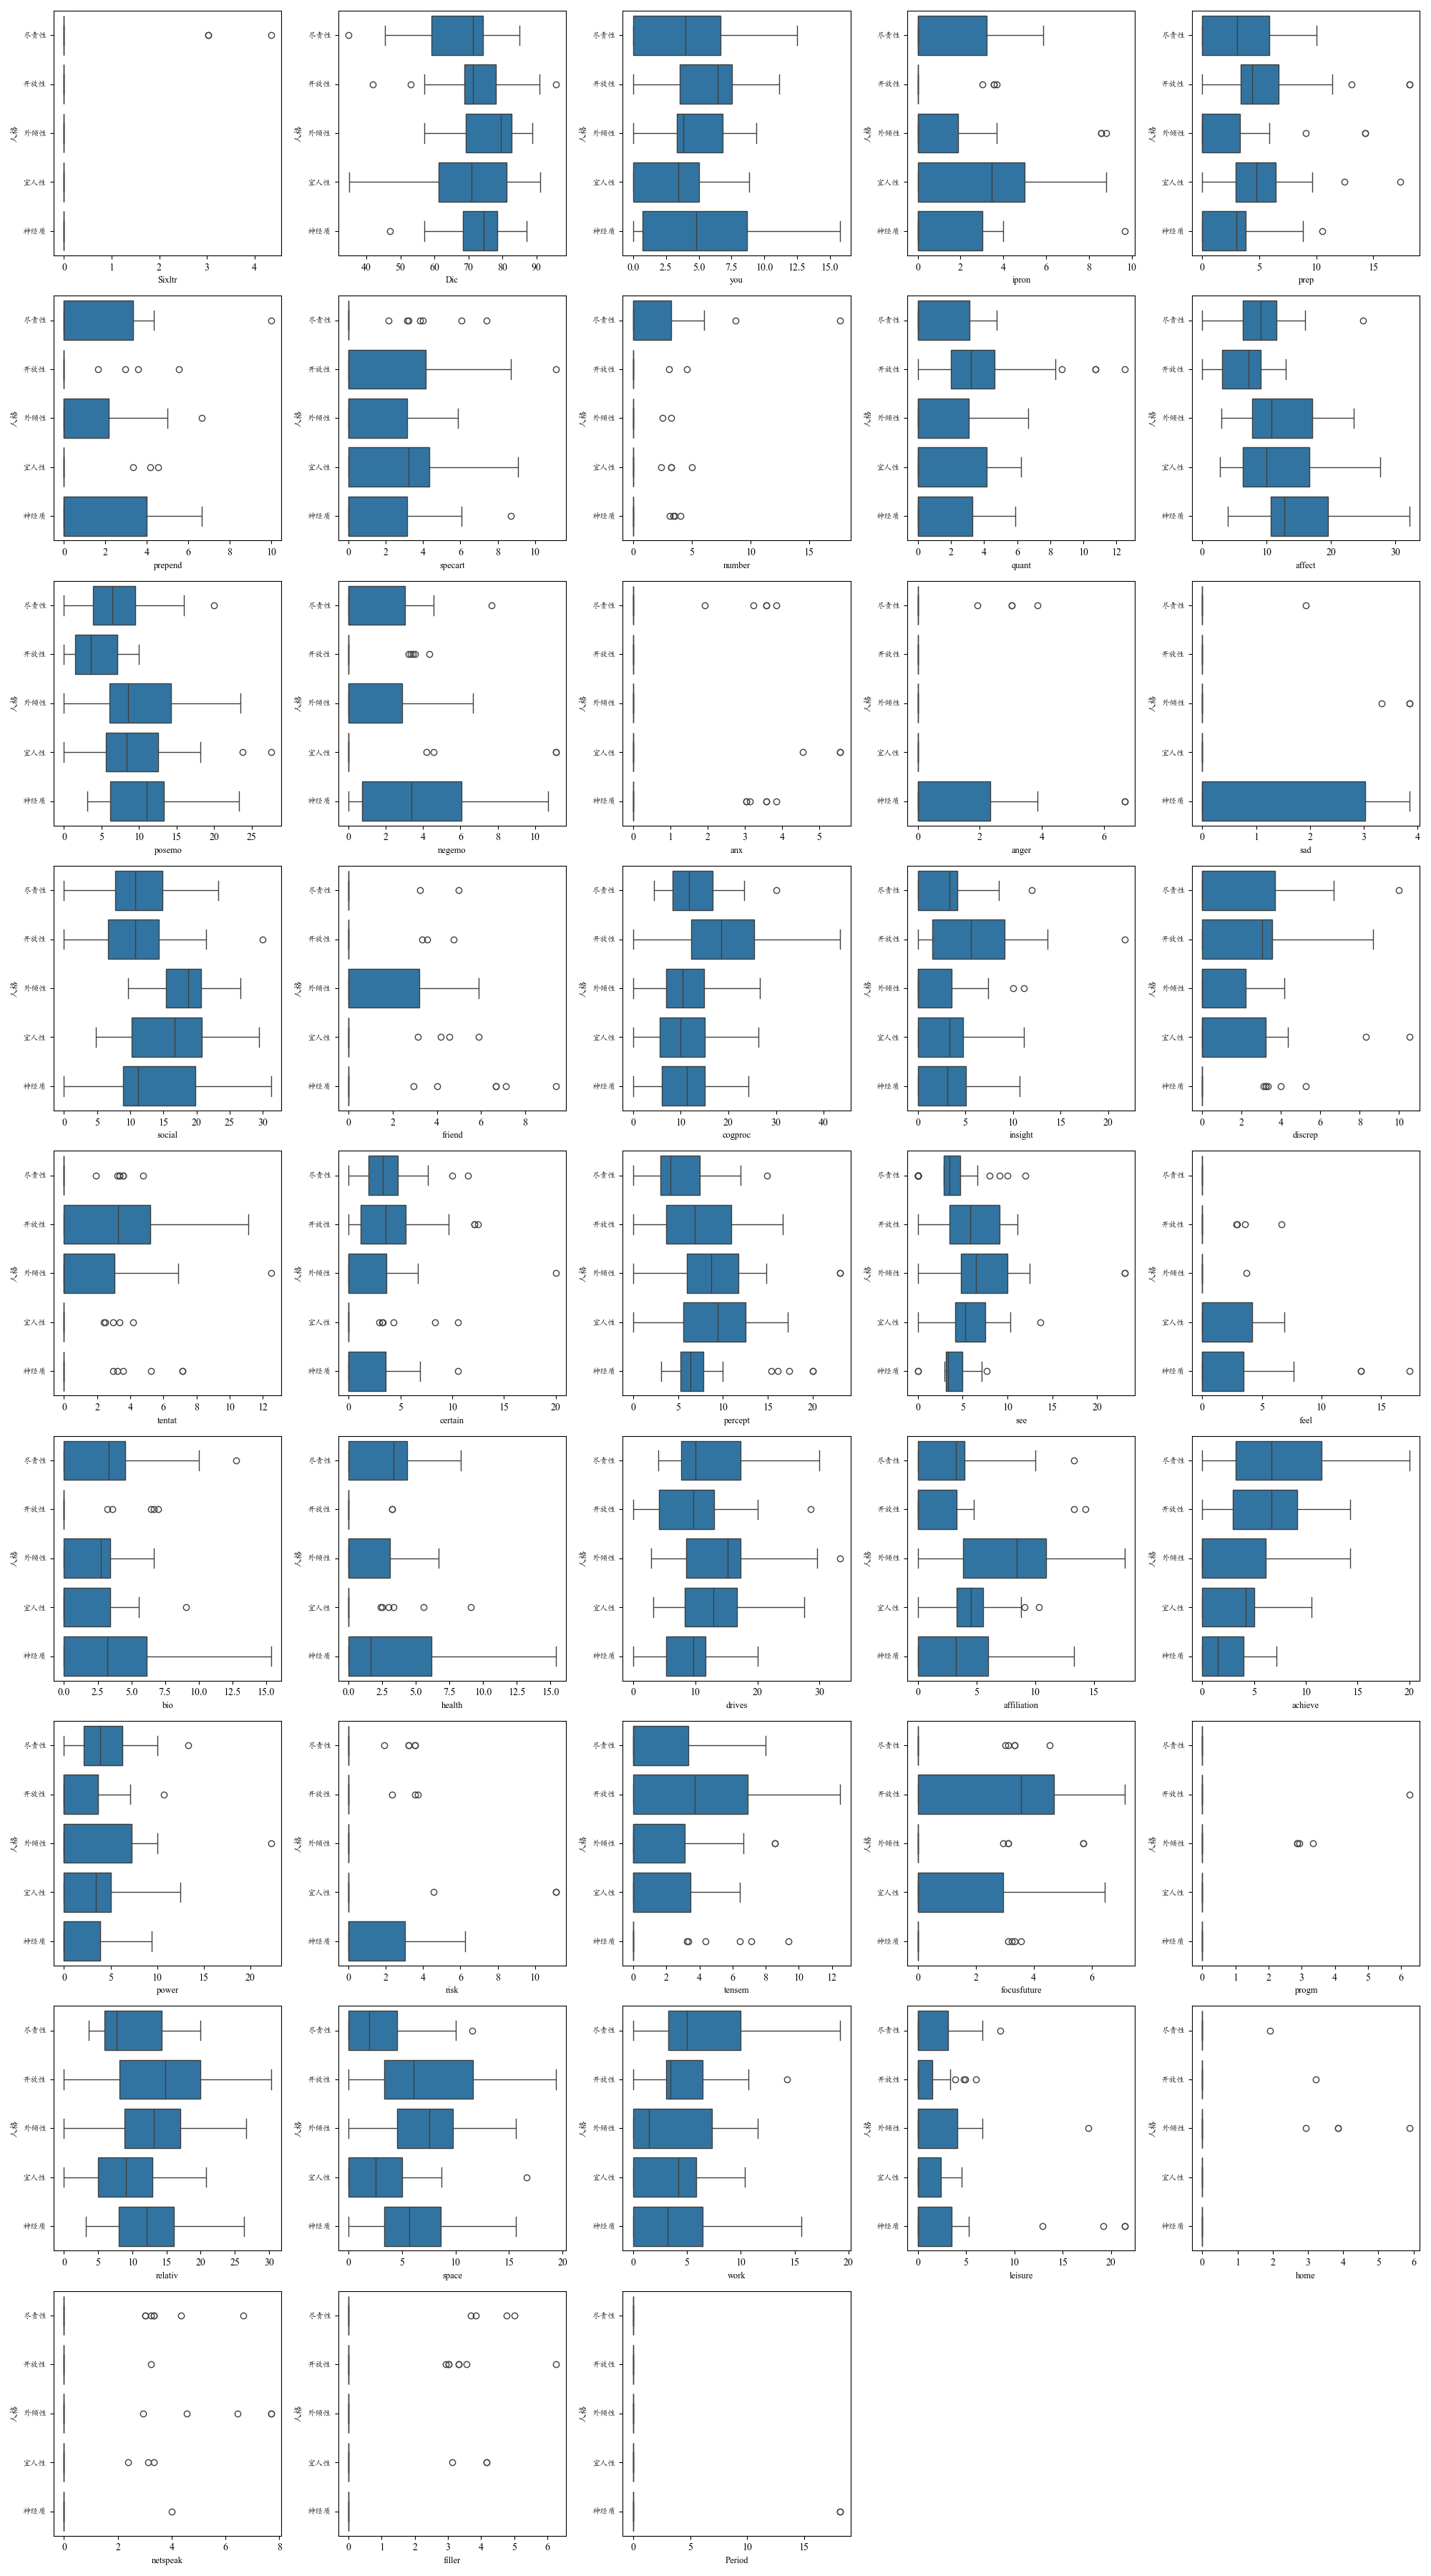
\includegraphics[width=0.8\linewidth]{Image/Study3-LIWC.png}
    \caption{\label{fig:Study3-LIWC}基于大五人格特质的个性化广告文本的语言特征分布}
\end{figure}

\textbf{外倾性}广告语言突出社交性与情感表达,符合外倾性人格的活跃与互动特质。外倾性广告中的社交相关词(social, \textit{F}(4,132) = 6.360, \textit{p} = 0.0001, 18.17\%)和归属动机词(affiliation, \textit{F}(4,132) = 9.840, \textit{p} < 0.001, 7.72\%)显著高于其他人格特质,体现出强烈的社交导向。此外,外倾性广告中的正面情感词(posemo, \textit{F}(4,132) = 7.181, \textit{p} < 0.001, 10.35\%)和感知词(percept, 9.32\%)的比例均为最高,进一步突出了积极、外向和注重体验的语言风格。

\textbf{宜人性}广告语言突出了情感温度和人际联结,体现了宜人性人格的共情与亲和特质。宜人性广告在正面情感词(posemo, 9.71\%)、社交相关词(social, 15.58\%)和归属动机词(affiliation, 4.75\%)方面均有较高占比,显示出广告内容偏向温暖、友好和关怀。此外,宜人性广告的语言风格也较为柔和,使用更多的情感相关词(affect, \textit{F}(4,132) = 8.942, \textit{p} < 0.001, 11.37\%)来增强情感连接。

\textbf{尽责性}广告语言风格注重目标导向和逻辑性,凸显了尽责性人格的计划性与成就驱动力。高尽责性广告中成就动机词(achieve, \textit{F}(4,132) = 6.710, \textit{p} = 0.0001, 7.32\%)使用最多,符合尽责性人格对成功和结果导向的关注。此外,尽责性广告在长词使用率(Sixltr, \textit{F}(4,132) = 2.898, \textit{p} = 0.0245)和数量词使用率(quant, \textit{F}(4,132) = 6.061, \textit{p} = 0.0002)上也显著高于其他特质,表现出语言上的正式性和条理性。

\textbf{开放性}广告文案呈现出鲜明的探索性与认知导向特征。高开放性广告在认知加工词(cogproc, \textit{F}(4,132) = 7.442, \textit{p} < 0.001, 19.60\%)和洞察词(insight, \textit{F}(4,132) = 3.829, \textit{p} = 0.0056, 5.93\%)的使用比例显著高于其他人格特质,反映了开放性人格偏好深入思考与探索的特质。此外,开放性广告大量使用空间相关词(space, \textit{F}(4,132) = 6.550, \textit{p} = 0.0001, 7.19\%)与感知词(percept, \textit{F}(4,132) = 3.321, \textit{p} = 0.0125, 7.74\%),表现出强调体验、探索与审美感知的语言风格。

\textbf{神经质}广告语言表现出显著的情绪波动与情感敏感特征。神经质广告中负面情感词(negemo, \textit{F}(4,132) = 7.308, \textit{p} < 0.001, 3.84\%)、焦虑词(anx, \textit{F}(4,132) = 2.845, \textit{p} = 0.0266, 0.78\%)、愤怒词(anger, \textit{F}(4,132) = 6.394, \textit{p} = 0.0001, 1.19\%)和悲伤词(sad, \textit{F}(4,132) = 8.058, \textit{p} < 0.001, 1.15\%)的使用均显著高于其他人格特质。这种情绪化的表达不仅强化了情感连接,也反映了神经质个体对情绪体验的高度敏感性。


在 LIWC 分析基础上,我们进一步通过词云图(图 \ref{fig:Study3-wordCloud})展示了五种人格特质广告的高频词。在制作词云图时,为突出各人格特质广告在语言风格上的差异,我们首先对五种人格个性化广告文本进行了预处理。具体而言,剔除了广告文本中未能体现人格特征且具有广泛通用性的高频词,例如“手机”“我们”“智能”等通用词汇。这些词语虽在广告中频繁出现,但主要源于广告语境和产品描述,与人格特质无直接关联,保留反而会掩盖不同人格特质在语言特征上的差异性。词云图中词语的大小代表其在对应人格广告中的出现频率,直观反映了各人格特质广告在语言风格上的差异。针对\textbf{外倾性}的广告,突出社交体验与分享感,词云中高频词如\textbf{“世界”“朋友”“分享”}与LIWC 中社交词(social)类别的高频结果一致,充分体现了外倾性个体偏好社交和互动的特质。\textbf{宜人性}广告强调情感共鸣与温暖体验,\textbf{如“美好”“温暖”“陪伴”}与 LIWC 中积极情感词(posemo)类别的高频结果相符,符合宜人性人格重视人际和情感连接的特点。\textbf{尽责性}广告则突出了功能性和可靠性,词云中的\textbf{“精准”“高效”“细节”}与 LIWC 中成就动机词(achieve)和认知加工词(cogproc)类别一致,契合尽责性人格偏好条理性和目标导向的特征。\textbf{开放性}广告则体现了探索与创造性的主题,高频词如\textbf{“创意”“探索”“无限”}与 LIWC 中感知类(percept)和洞察类词(insight)的高频结果相符,反映了开放性人格追求新体验和创造力的偏好。\textbf{神经质}广告则着重于情感安抚与安全感,\textbf{“陪伴”“温暖”“放松”}如,与 LIWC 中负面情感词(negemo)、焦虑词(anx)及亲和性词(affiliation)的显著性结果一致,突出了神经质人格在情绪波动中对安全感和情感支持的需求。

综合 LIWC 分析与词云可视化结果,本研究揭示了不同人格特质广告在语言特征上的显著差异,充分展现了基于大五人格模型的个性化广告语言模式。这一结果不仅丰富了对个性化广告语言特征的理解,也进一步验证AI基于人格特征生成个性化广告文本的能力。

\begin{figure}[H]
    \centering
    % 第一行三张图
    \subfloat[外倾性]{
        
\includegraphics[width=0.2\linewidth]{Image/Study3-外倾性.png}
    }\hspace{1em}
    \subfloat[宜人性]{
        
\includegraphics[width=0.2\linewidth]{Image/Study3-宜人性.png}
    }\hspace{1em}
    \subfloat[尽责性]{
        
\includegraphics[width=0.2\linewidth]{Image/Study3-尽责性.png}
    }
    \\[1em] % 换行并增加垂直间距
    % 第二行两张图
    \subfloat[开放性]{
        
\includegraphics[width=0.2\linewidth]{Image/Study3-开放性.png}
    }\hspace{2em}
    \subfloat[神经质]{
        
\includegraphics[width=0.2\linewidth]{Image/Study3-神经质.png}
    }
    \caption{\label{fig:Study3-wordCloud}基于大五人格特质的个性化广告文本词云图}
    \label{fig:personality_images}
\end{figure}


\section{子研究二:个性化广告效果模型构建} 
在研究一和研究二中,个性化广告的效果评估主要依赖实验数据。尽管 AI 生成技术显著降低了实验材料的制作成本,使大规模生成个性化广告成为可能,但广告效果的验证仍需大量被试,并要求他们填写人格问卷,以匹配个性化广告的目标群体。然而,这种基于实验的方法不仅在时间和资源上存在限制,难以实现快速评估,还需要依赖受试者的参与,因而在实际应用中具有一定局限性。因此,构建预测模型能够提供一种更高效的评估手段,使研究者或广告实践者在广告发布前预测其对不同人格特质群体的吸引力。这不仅有助于降低实验成本,还能在广告投放前优化个性化策略,从而提高广告匹配度和转化率。此外,在前述研究中,我们已收集了大量基于 AI 生成的广告文本,并获得了带有个性化特质信息的被试评分数据,使得构建个性化广告说服效果模型成为可能。尽管实验中的广告是围绕某一特定人格特质(如高外倾性、高开放性等)进行定制的,但广告文本可能包含多层次的语言元素,使其不仅对目标特质群体有效,也可能吸引其他人格特质的个体。例如,一个为高开放性个体设计的广告可能突出探索性与创造力,但其中的情感化或社交化表达同样可能对高宜人性或高外倾性的个体产生吸引力。因此,在模型构建过程中,我们不仅考察广告在目标特质群体中的说服效果,还计算该广告对其他人格特质个体的吸引程度。这一方法突破了传统个性化广告评估仅关注目标群体的局限,使得模型能够更全面地预测个性化广告在不同人格特质群体中的适用范围,为广告优化和投放策略提供更具适应性的参考。综上所述,子研究二基于前述实验的实验材料和数据,结合LIWC语言特征,构建个性化广告效果的预测模型。

\subsection{方法}

\subsubsection{建模数据}

\textbf{(1)数据来源}

本研究的模型构建基于研究一和研究二的实验数据,涵盖 AI 生成与人类专家创作的个性化广告文本及其参与者评分。所有实验均采用大五人格测量工具(BFI-10 或 BFI-44)评估参与者的人格特质,并要求他们对不同个性化广告文本进行评分。为确保模型能够准确评估广告对不同人格特质群体的吸引力,我们优先选取完成完整人格测量的实验数据,以提高个性化说服效果计算的精度。具体而言,模型训练数据整合了多个实验的数据集(详见表 \ref{tab:model_data}),每名参与者在实验中评价 5 条广告,而每条广告的最终评价人数因实验条件不同而有所变化。经过筛选,最终用于模型训练的广告样本共计112条。

\begin{table}[htbp]
    \centering
    \caption{\label{tab:model_data} 建模数据来源}
    {\tablesongti % 整个表格环境应用宋体六号字体
    \renewcommand{\arraystretch}{1.5} % 调整行距
    \begin{tabular}{p{2cm} p{2cm} c c c} % 控制列宽
        \toprule
        \textbf{实验} & \textbf{人格测量量表} & \textbf{参与者人数} & \textbf{每名受试者评价文本数} & \textbf{单条广告评价人数} \\
        \midrule
        研究一-实验1 & BFI-10 & 192 & 5 & 65 \\
        研究二-实验1 & BFI-10 & 322 & 5 & 32--59 \\ % 使用 -- 代替 –
        研究二-实验2 & BFI-44 & 368 & 5 & 13--68 \\ % 使用 -- 代替 –
        \bottomrule
    \end{tabular}
    }
\end{table}




\textbf{(2)计算方法}
\label{calculationMethods}

为构建模型,我们对个性化广告的说服效果进行了量化处理。计算过程分为\textbf{个体层面}和\textbf{广告层面}。

在\textbf{个体层面},我们首先对每名受试者在实验中的广告评分进行标准化,以消除个体评分偏差。随后,将个体的人格得分也进行标准化,并计算个体在所有广告上的评分与其在人格上的偏离程度,以衡量特定人格水平个体对广告的偏好倾向。具体计算如下,其中,\( S_{\text{ad},i} \) 代表个体 \( i \) 在某条广告上的评分,\( \mu_{S,i} \) 和 \( \sigma_{S,i} \) 分别为该个体在所有广告上的评分均值和标准差。类似地,\( P_{i} \) 代表个体 \( i \) 在该人格特质上的得分,\( \mu_{P} \) 和 \( \sigma_{P} \) 分别为该特质在所有被试中的均值和标准差。

\begin{equation}
    Z_{\text{ad},i} = \frac{S_{\text{ad},i} - \mu_{S,i}}{\sigma_{S,i}}, \quad
    Z_{\text{trait},i} = \frac{P_{i} - \mu_{P}}{\sigma_{P}}
    \label{eq:standardization}
\end{equation}

然后,在\textbf{广告层面},计算个体对广告的个性化说服效应。我们将所有被试对某条广告的个性化说服效应 \( P_{\text{ad},i} \) 进行累加,得到该广告针对特定人格特质的个性化说服指数,如公式\eqref{eq:persuasion_effect} 所示。其中,\( P_{\text{ad}} \) 的正值表示高水平特质个体更偏好该广告,低水平特质个体更不偏好(即高水平个性化说服效果较强);而负值则表示低水平特质个体更偏好该广告,高水平特质个体更不偏好(即低水平个性化说服效果较强)。

\begin{equation}
    P_{\text{ad},i} = Z_{\text{ad},i} \times Z_{\text{trait},i}
    \label{eq:persuasion_effect}
\end{equation}

\begin{equation}
    P_{\text{ad}} = \sum_{i=1}^{N} P_{\text{ad},i}
    \label{eq:persuasion_index}
\end{equation}


\subsubsection{模型选择}
在本研究中,我们选用了随机森林(Random Forest)作为个性化广告说服效果的预测模型。这一选择主要基于其在处理高维数据、特征选择、非线性建模以及对小样本数据的适应性等方面的优势,使其特别适用于文本特征驱动的预测任务。本研究的自变量来源于广告文本的语言特征,因变量则为该广告在不同人格群体中的个性化说服效果。文本特征采用LIWC(Linguistic Inquiry and Word Count)分析得到,涵盖多个维度,如情感(情绪正负性)、认知(推理、因果分析)、社交(人称代词、社交相关词汇)以及驱动(成就动机、亲和动机等)。由于广告文本包含多个层面的语言元素,个性化广告的说服效果可能受到不同语言特征的复杂影响。因此,我们需要一种既能处理高维数据、又能捕捉非线性关系的建模方法,以提高个性化广告预测的准确性。

随机森林模型在这一任务中具有显著优势。首先,它适用于高维特征数据。在文本分析任务中,自变量往往由多个语言特征构成,且不同特征可能存在较强的相关性。相比传统回归模型,随机森林能够在众多特征中自动选择最具预测价值的变量,而不会受到多重共线性问题的困扰。同时,其集成学习机制通过多个决策树的组合,减少了单一模型可能出现的过拟合问题,从而提升泛化能力。

其次,随机森林具备强大的特征选择能力。在个性化广告预测任务中,我们希望不仅能够预测广告的说服效果,还能识别哪些文本特征最具影响力。随机森林能够通过计算特征重要性,如基尼指数(Gini Importance)或置换重要性(Permutation Importance),评估每个文本特征对说服力的贡献。这一特性使得我们能够深入分析不同语言特征在个性化广告中的作用,并据此优化广告文案的个性化策略。

此外,个性化广告的说服效果可能受到多种复杂因素的共同影响。例如,词汇的多样性可能在一定程度上提升广告吸引力,但过度复杂的表达可能降低可读性,从而影响说服效果;具有情感共鸣的语言可能对某些人格特质的个体有效,但对其他群体则可能适得其反;认知类词汇(如逻辑推理、因果分析)可能增强信息可信度,但对低开放性个体来说可能较难理解。相较于线性回归或普通决策树,随机森林能够灵活捕捉这些非线性模式,使得预测模型更贴合文本特征与个性化广告效果之间的真实关系。

另一个关键优势是随机森林对异常值和噪声的鲁棒性。由于文本数据可能包含噪声(如广告文案中的冗余词汇)、极端值(如某些特征的异常高频)或缺失值,随机森林的集成学习方式能有效降低单一异常值对整体预测结果的影响。多个决策树的投票机制确保了模型的稳定性,使其在数据质量不完美的情况下仍能保持较好的预测性能。

最后,随机森林在小样本和不平衡数据下仍能稳定表现。个性化广告的实验数据相较于典型的自然语言处理(NLP)任务而言,规模相对较小,且不同人格特质的受试者分布可能存在不均衡。随机森林的随机采样(Bootstrap Sampling)机制使其能够更好地利用有限数据,并通过集成多个弱学习器提升模型的泛化能力。

\subsubsection{模型训练}
在本研究中,我们采用随机森林分类器(Random Forest Classifier)对个性化广告的说服效果进行建模与训练。模型训练的主要目标是基于广告文本的语言特征,预测该广告在特定人格特质群体中的说服力。具体而言,我们针对大五人格的每个维度分别训练一个分类模型,以评估广告文本在不同人格群体中的个性化效果。在模型训练过程中,我们首先对数据进行划分。对于每个目标人格特质(如开放性、尽责性等),自变量X由 LIWC 语言特征组成,因变量y代表该广告在该人格特质上的个性化说服效果(计算方法详见\ref{calculationMethods})。由于个性化说服得分是一个连续变量,为构建分类模型,我们将其转换为二分类标签:

\begin{equation}
y =
\begin{cases}
1, & P_{\text{ad}} \geq 0 \quad \text{(广告更受高水平特质个体偏好)} \\
0, & P_{\text{ad}} < 0 \quad \text{(广告更受低水平特质个体偏好)}
\end{cases}
\end{equation}

这样,我们的分类模型即可预测某则广告是否更符合高水平特质个体的偏好模式。为确保模型的稳健性,我们将数据集按照7:3的比例划分为训练集(70\%)和测试集(30\%),并采用分层抽样,使得训练集和测试集中各人格特质水平的分布保持一致,以减少类别不均衡对模型的影响。

在训练过程中,我们采用两阶段建模策略,即先训练基础随机森林模型,再利用该模型进行特征选择,以筛选出最具预测价值的语言特征。首先,我们使用100 棵决策树(n\_estimators=100)训练一个初始随机森林分类器,并利用其特征重要性来进行变量筛选。具体而言,我们基于平均特征重要性设定筛选阈值,仅保留重要性高于均值的特征,从而减少冗余信息,提高模型的泛化能力。随后,我们使用筛选后的特征重新训练最终的随机森林分类器,以进一步优化预测性能。训练完成后,我们在测试集上评估模型性能,并计算准确率以衡量模型的预测能力。

\subsection{结果}

\textbf{(1)模型预测结果}

图 \ref{fig:prediction_accuracy} 展示了基于随机森林模型对不同人格特质个性化广告的预测准确率。纵轴表示预测准确率,横轴为五种人格特质(宜人性、外倾性、开放性、尽责性、神经质)。从结果来看,尽责性广告的预测准确率最高(0.76),其次为神经质(0.66)、宜人性(0.65)、外倾性(0.62),而开放性广告的预测准确率最低(0.59)。其中,图中的虚线表示随机水平(即 0.50),若预测准确率高于该水平,说明模型的预测优于随机猜测。整体而言,模型在不同人格特质上均表现出一定的预测能力,尤其是在尽责性广告上的预测效果最佳。这可能与尽责性个性化广告的语言特征更加稳定、可预测性更高有关,而开放性广告的预测效果相对较低,可能是由于其语言风格更加多样化,导致模型难以捕捉固定模式。

\begin{figure}[H]
    \centering
    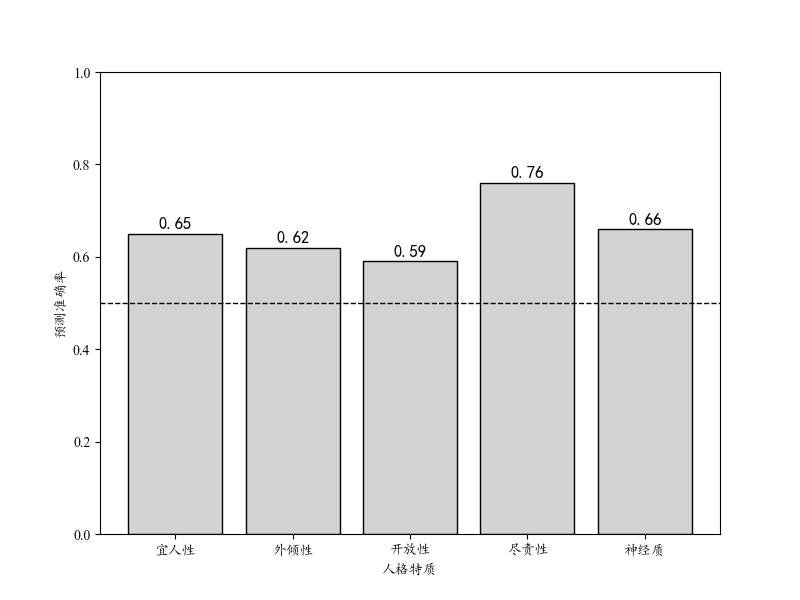
\includegraphics[width=1\linewidth]{Image/Study3-predictionAccuray.png}
    \caption{\label{fig:prediction_accuracy}模型预测准确率}
\end{figure}

为进一步解析个性化广告预测模型中语言特征的作用,本研究引入 SHAP(SHapley Additive exPlanations) 方法对特征贡献进行分析。SHAP 是一种基于 Shapley 值的模型解释方法,被广泛用于评估机器学习模型中各特征对预测结果的贡献。其核心思想是计算每个特征在不同预测情境下的边际贡献,从而提供一致且可解释的特征重要性衡量标准。相比于传统的特征重要性计算方法(如随机森林中的 Gini 重要性或基于置换的重要性分析),SHAP 具有更强的理论可解释性,能够有效捕捉特征间的交互效应,使研究者能够更全面地理解模型的决策过程。

\textbf{(2)特征贡献度}

在本研究中,我们针对五种人格特质(宜人性、外倾性、开放性、尽责性、神经质)分别计算 SHAP 值,以解析不同语言特征在个性化广告预测任务中的贡献。SHAP 值的正负表示该特征对模型预测结果的影响方向:正 SHAP 值表示该特征增加了高水平特质个体偏好的预测概率,而负 SHAP 值则表示该特征更倾向于预测低水平特质个体的偏好模式。此外,SHAP 值的绝对大小反映了该特征的重要性,即数值越大,说明该特征对模型预测的影响越显著。图 \ref{fig:featureHeatmap} 展示了 SHAP 计算得到的特征重要性热力图,横轴表示人格特质类别,纵轴为 LIWC 语言特征,颜色深浅表示该特征在相应人格特质预测任务中的贡献大小。

从 SHAP 计算结果来看,不同人格特质的个性化广告在语言特征上表现出一定的模式。例如,在 \textbf{尽责性} 个性化广告的预测模型中,\textit{drives}(动机相关)、\textit{work}(工作相关)和\textit{quant}(数量表达)等特征的重要性最高,这与尽责性个体强调目标导向、任务执行和条理性的特点一致。同时,\textit{negemo}(负面情绪)特征在尽责性广告预测中也表现出较高 SHAP 贡献,这可能是由于尽责性个体在广告内容中更关注潜在风险或任务挑战,从而影响其对广告的接受度。

在 \textbf{外倾性} 个性化广告的预测模型中,\textit{social}(社交相关)、\textit{posemo}(正面情绪)和\textit{reward}(奖励)等特征的重要性较高,表明外倾性个体更倾向于被强调社交互动、正向体验和激励机制的广告所吸引。此外,\textit{you}(第二人称代词)的贡献也较大,可能表明外倾性个体更偏好直接互动式的广告表达。

\textbf{宜人性} 个性化广告的预测模型则显示,\textit{compare}(比较)、\textit{motion}(运动相关)和\textit{feel}(情感相关)等特征的重要性较高。这表明宜人性个体在广告中更关注人与人之间的关系、情感共鸣以及相对评价,而\textit{pronoun}(代词)的贡献也说明宜人性广告可能更倾向于使用第一人称或第三人称代词,以增强广告的亲和力和人际互动。

\textbf{神经质} 个性化广告的预测模型中,\textit{negemo}(负面情绪)、\textit{tentat}(不确定性)和\textit{risk}(风险)等特征的重要性最高。这表明神经质个体更倾向于受到涉及焦虑、不安和不确定性表达的广告影响,同时也可能偏好那些能够提供安全感和情绪安抚的信息。此外,\textit{social}(社交相关)特征在神经质个体的广告预测中也具有较高贡献,这可能是由于该群体更容易受到社交焦虑或社交互动内容的影响。

相比之下,\textbf{开放性} 个性化广告的预测模型中,各特征的 SHAP 贡献较为分散,缺乏单一主导特征。这可能与开放性人格本身的语言风格高度多样化有关。例如,\textit{informal}(非正式表达)、\textit{cause}(因果逻辑)、\textit{cogproc}(认知过程)和\textit{compare}(比较)等特征在开放性广告预测中均有所贡献,但整体重要性不如其他人格特质广告任务中的显著。这一结果可能表明,开放性广告的个性化表达方式较为宽泛,使得模型难以精准捕捉统一的语言模式。

综合来看,SHAP 分析进一步支持了 LIWC 语言特征在个性化广告预测中的作用,并揭示了不同人格特质在语言表达上的独特性。尽责性、外倾性和宜人性广告的语言特征较为稳定,使得模型能够较准确地预测个性化广告效果,而开放性广告由于语言多样性较高,可能导致预测性能的下降。这一发现不仅为 AI 生成个性化广告的优化提供了数据支持,也为未来在个性化广告设计中更精细地调整语言策略提供了理论依据。

\begin{figure}[H]
    \centering
    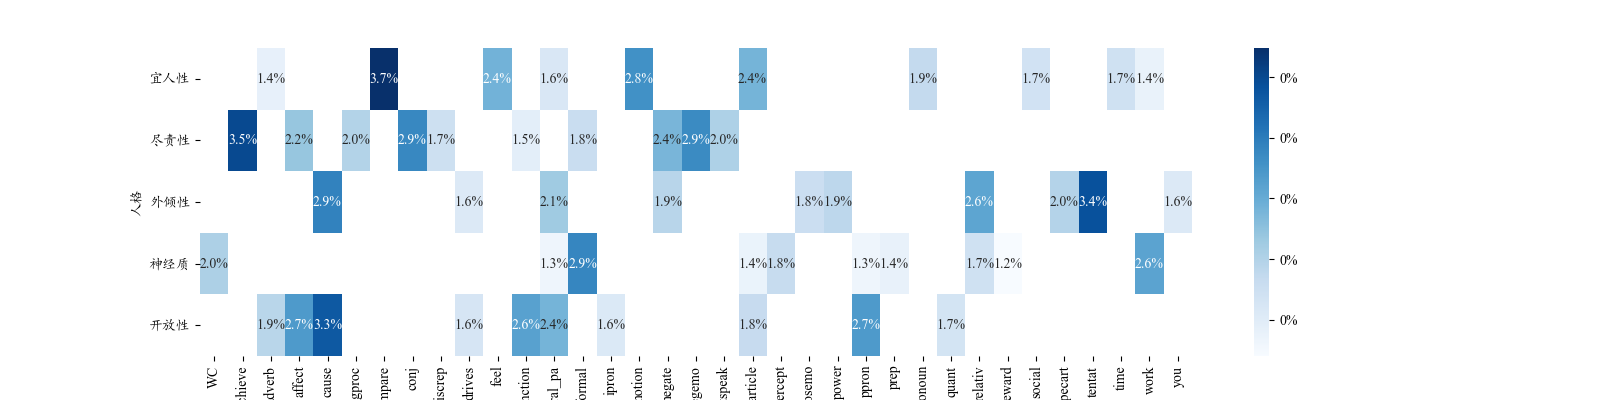
\includegraphics[width=1.2\linewidth]{Image/Study3-heatmap.png}
    \caption{\label{fig:featureHeatmap}特征SHAP值热力图}
\end{figure}

\textbf{(3)高水平vs低水平偏好特征差异}

在本研究中,我们基于参与者的实际广告评分计算了个性化说服效应(计算方法详见 \ref{calculationMethods}),衡量不同人格特质水平的个体对广告内容的偏好模式。相较于子研究一仅关注高水平特质广告文本的语言特征(§ \ref{study3-substudy1}),本研究中进一步分析高低水平人格特质个体在广告语言特征上的偏好差异。通过独立样本t检验比较高水平与低水平个体在LIWC 语言特征偏好上的显著性差异,并计算 Cohen’s d以评估效应量。这一分析不仅揭示了高低水平个体在广告接受度上的语言特征偏好,还为优化个性化广告的匹配策略提供了新的视角。

高宜人性个体更偏好包含 \textbf{比较(compare)} 词汇的广告 \((t = 3.13, p = 0.002, d = 0.59)\),并且在\textbf{代词(pronoun)} 使用上显著更高 \((t = 2.65, p = 0.009, d = 0.50)\)。这表明,高宜人性个体更倾向于接受\textbf{强调个体差异、相对优势} 的广告,例如:“你的时间宝贵,所以我们的手机不容许任何延误。一键快速响应,确保每一秒都计算得刚刚好。” 此外,高宜人性个体对\textbf{未来导向(focusfuture)} 的内容表现出更高的接受度 \((t = 1.97, p = 0.052, d = 0.37)\),说明他们更偏好\textbf{强调长期利益和积极愿景} 的广告表达。低宜人性个体更偏好\textbf{否定(negate)} \((t = -2.04, p = 0.044, d = -0.39)\) 和\textbf{愤怒(anger)} \((t = -2.01, p = 0.049, d = -0.39)\),表明他们对\textbf{直接、批判性更强的广告} 反应更积极,如:“你的朋友已为此狂热,这不仅是手机,更是社交的新纪元。展现个性,享受交流,无限精彩尽在掌中。” 此外,低宜人性个体对\textbf{生物相关词汇(bio,如“健康”“身体”)} 更敏感 \((t = -2.15, p = 0.035, d = -0.42)\),这可能意味着他们更容易被\textbf{与身体机能、健康维护相关的广告} 吸引,如:“智能调节屏幕色温,缓解视疲劳,让工作休闲更加舒适。”

高开放性个体在\textbf{代词(ppron)} \((t = 2.91, p = 0.004, d = 0.55)\) 和\textbf{功能词(function words)} \((t = 2.26, p = 0.026, d = 0.43)\) 的使用上显著更高,表明他们更倾向于接受\textbf{强调个体体验、社交互动,或富有思辨性的广告表达},例如:“使用这款手机,你将体验到最全新的技术、最前卫的设计;在这里,你将以从未想象过的方式探索手机的世界。” 此外,高开放性个体更偏好\textbf{强调集体归属感} 的语言,他们更常被包含 \textbf{“我们”(we)} 的广告所吸引 \((t = 2.06, p = 0.042, d = 0.39)\),如:“共同追求进步,创造美好的明天。手机作为你的工具,与你一同实现梦想。” 低开放性个体更偏好\textbf{数字(number)} \((t = -1.93, p = 0.058, d = -0.36)\),说明他们更倾向于\textbf{基于数据、事实支撑的广告},例如:“99\% 的用户推荐,实验数据显示出色性能。”

高尽责性个体更偏好\textbf{功能词(function)} \((t = 2.70, p = 0.008, d = 0.52)\) 和\textbf{未来导向(focusfuture)} \((t = 1.83, p = 0.070, d = 0.34)\),表明他们更容易接受\textbf{逻辑清晰、目标导向的广告},例如:“精准定位,发现生活中的美好细节。捕捉时刻,记录珍贵瞬间。” 低尽责性个体更偏好\textbf{否定(negate)} \((t = -2.54, p = 0.013, d = -0.50)\) 和\textbf{负面情绪词汇(negemo)} \((t = -2.46, p = 0.016, d = -0.47)\),说明他们更容易被\textbf{强调挑战、失败或压力} 的广告吸引,如:“如果你不立即采取行动,你可能会错失机会。”

高外向性个体更偏好\textbf{相对性词汇(relativ,如“更快”“更高”)} \((t = 2.58, p = 0.011, d = 0.49)\) 和\textbf{不确定性表达(tentat,如“可能”)} \((t = 2.45, p = 0.016, d = 0.46)\),他们更容易接受\textbf{强调探索性、互动感的广告},如:“翻阅朋友的动态,把温馨的友情牢牢捕捉。” 低外向性个体 更偏好\textbf{权力(power)} 相关词汇 \((t = -2.08, p = 0.041, d = -0.40)\),表明他们更倾向于\textbf{强调掌控感、决策权威性的广告},如:“你的时间宝贵,所以我们的手机不容许任何延误。”

高神经质个体偏好\textbf{网络用语(netspeak)} \((t = 2.00, p = 0.050, d = 0.40)\),表明他们更容易接受\textbf{非正式、口语化的广告风格},如:“在欢笑中,她是你探索世界的桥梁;在泪水中,她是你疗愈伤痕的港湾。” 低神经质个体更偏好\textbf{未来导向(focusfuture)} \((t = -3.03, p = 0.003, d = -0.57)\),这表明他们更倾向于\textbf{强调长期规划、稳定性的广告},如:“开启智慧生活,助你成为更好的自己。”

\section{讨论} 

本研究通过文本分析和预测建模,深入探讨了个性化广告文本的语言特征及其对广告说服效果的影响。研究三的结果表明,不同人格特质的个性化广告在语言风格上存在系统性差异 \citep{koutsoumpis2022kernel},且这些差异能够有效预测广告的个性化说服效果。此外,本研究进一步比较了 AI 生成的个性化广告文本特征 与 不同人格特质个体在实际偏好中表现出的语言特征,揭示了 AI 在个性化广告生成中的局限性。尽管 AI 在广告设计时基于各特质的语言风格进行针对性优化,但由于语言使用在不同情境下可能呈现不同特征,即使是同一人格特质,针对不同广告类型,其语言风格也可能存在显著差异 \citep{flores2014effect},AI 在个性特质与广告场景的结合方面仍然存在短板。此外,以往研究主要关注高水平特质的语言偏好,而对低水平特质的个性化偏好探讨较少,本研究的结果表明,低水平特质个体的广告偏好并不完全符合传统人格特质的解读,而在广告情境下表现出新的特征倾向。例如,某些低水平特质个体偏好的特征与其在一般语言研究中的表现不完全一致,这表明个性化广告的说服机制可能受到额外的语境因素影响。这些发现不仅反映了 AI 生成广告在低水平特质个性化匹配上的挑战,也为未来个性化广告优化提供了新的方向。因此,未来的个性化广告生成需要更加关注语言风格在不同语境中的适应性,并结合高低水平特质的实际偏好,以提高个性化匹配的精准度和广告的说服力。接下来将从各人格特质展开,进一步讨论 AI 生成文本与实际个性化偏好的具体差异,并探讨其可能的成因及优化方向。

在\textbf{外倾性}个性化广告的设计中(如表 \ref{tab:study3_extraversion_comparison}),AI 主要关注的是社交互动、情感表达和积极体验,因此生成的广告文本往往包含大量社交相关(social)和正面情感(posemo)词汇,例如“与世界分享你的热情,记录美好时刻,激发他人的快乐与欢笑”。此外,外倾性广告通常也会使用感知类(percept)词汇,以增强体验感。然而,从外倾性参与者的实际反馈来看,尽管这些元素符合外倾性个体的语言风格,但更能提升个性化广告效果的特征还包括激励性表达(reward)和互动性用语(you),如“你的朋友已为此狂热,这不仅是手机,更是社交的新纪元”。相比之下,AI 在生成广告时虽然强调了社交主题,但可能低估了“互动”在广告场景中的重要性。造成这一偏差的一个可能原因是,大多数关于人格与语言的研究侧重于个体的自然语言表达习惯,而不是他们在广告情境下的偏好。外倾性个体的日常语言确实包含更多社交词汇,但这些表达通常是针对社交情境,而非广告语境。在广告场景中,外倾性个体可能更倾向于被直接卷入对话,需要更多“你”(you)的参与感,而不仅仅是对“社交”概念的描述。因此,AI 在广告生成时,应考虑如何从社交语言风格转向“交互式”语言设计,例如采用问题导向、邀请式的表达(如“你将如何使用这款手机?”),以进一步增强广告的吸引力。此外,低外倾性个体的广告偏好与传统外倾性/内倾性语言风格的理解并不完全一致。通常,低外倾性个体在自然语言表达中更偏向于内省、个体化、秩序感,但在广告场景下,他们更倾向于强调权力和掌控感的广告,如“精准管理你的时间,高效完成每一个任务”。这可能表明他们对社交互动的关注度较低,而更希望广告提供增强个人自主性的承诺。这与研究发现的低外倾性个体更喜欢反思、更注重个体控制,并倾向于结构化和秩序化的生活一致 \citep{beukeboom2013language}。这一发现说明,在个性化广告的设计上,AI 不应仅停留在基于人格特质的表层语言特征,而应深入挖掘不同人格特质的更深层次需求,特别是在特定广告情境下如何有效激发不同群体的兴趣和认同感。


\begin{table}[H]
    \centering
    \caption{\label{tab:study3_extraversion_comparison} 高外倾与低外倾的个性化广告语言特征偏好}
    {\tablesongti % 整个表格环境应用宋体六号字体
    \renewcommand{\arraystretch}{1.5} % 调整行距
    \begin{tabularx}{\linewidth}{l X X} % 设定每列宽度
        \toprule
        \textbf{外倾性} & \textbf{AI 生成} & \textbf{实际偏好} \\
        \midrule
        \multirow{5}{*}{\textbf{高外倾}} 
        & 社交相关(social),如“与世界分享你的激情” & 社交相关(social),如“你的朋友已为此狂热” \\
        & 正面情感(posemo),如“让你的社交世界明亮而充满希望” & 正面情感(posemo),如“激发他人的快乐与欢笑” \\
        & 感知体验(percept),如“感受科技带来的精彩” & 感知体验(percept),如“探索全新体验” \\
        &  & \textcolor{red}{互动性(you),如“你将如何使用?”} \\
        &  & \textcolor{red}{激励性表达(reward),如“开启你的无限可能”} \\
        \midrule
        \multirow{5}{*}{\textbf{低外倾}} 
        & \multirow{5}{*}{样本不足未分析}  & 强调个人自主(individuality),如“精准管理你的时间” \\
        &  & 掌控感(control),如“助你高效决策” \\
        &  & 秩序、结构化表达(order),如“让你的生活井然有序” \\
        &  & 权力(power),如“主宰你的生活节奏” \\
        \bottomrule
    \end{tabularx}
    }
\end{table}


在\textbf{宜人性}个性化广告的设计上(如表 \ref{tab:study3_agreeableness_comparison}),AI 主要强调温暖、关怀和归属感,因此生成的广告往往包含较多积极情感(posemo)、社交相关(social)和归属动机(affiliation)词汇,如“用这款手机,把温情传递给每一个需要的角落”。然而,实际广告偏好表明,他们还更加看重比较性表达(compare)和未来导向(focusfuture),例如“精准生活,从不间断”。这一点可能源于高宜人性个体在社交互动中不仅关注情感连接,还关注相对优势和长远利益,他们希望看到广告内容如何凸显产品在人际关系或个人体验中的独特性。这一偏好与以往研究对宜人性个体的理解有所不同,因为过往研究多强调宜人性与和谐沟通的关系,而本研究的结果表明,在广告场景中,高宜人性个体更关注产品的竞争力,以及产品如何带来持续性的价值。而对于低宜人性个体,在实际偏好中更倾向于直接、批判性更强的语言风格,如否定性表达(negate)和愤怒(anger)。此外,他们还对生物相关内容(bio) 产生了更高的偏好,这表明低宜人性个体可能更关注产品对个人生理需求的直接影响,而不是对社交关系的促进。这与传统研究强调低宜人性个体更直接较少关注情感交流和他人感受的特征一致 \citep{crowe2018uncovering}。未来的个性化广告设计应考虑,针对低宜人性个体,广告可以减少冗余的情感表达,而更加强调产品的物理性能、个人体验和问题解决能力,例如“强劲性能,不再忍受卡顿”或“守护你的健康,关心你的身体”。

\begin{table}[H]
    \centering
    \caption{\label{tab:study3_agreeableness_comparison} 高宜人性与低宜人性的个性化广告语言特征偏好}
    {\tablesongti % 整个表格环境应用宋体六号字体
    \renewcommand{\arraystretch}{1.5} % 调整行距
    \begin{tabularx}{\linewidth}{l X X} % 设定每列宽度
        \toprule
        \textbf{宜人性} & \textbf{AI 生成} & \textbf{实际偏好} \\
        \midrule
        \multirow{4}{*}{\textbf{高宜人性}} 
        & 积极情感(posemo),如“用这款手机,把温情传递给每一个需要的角落” & 积极情感(posemo),如“用这款手机,把温情传递给每一个需要的角落” \\
        & 社交相关(social),如“记录美好瞬间,让善意的温暖传递到每个角落” & 社交相关(social),如“记录美好瞬间,让善意的温暖传递到每个角落” \\
        & 归属动机(affiliation),如“与世界分享你的温暖,让每一次沟通都更有意义” &  \textcolor{red}{比较(compare),如“精准生活,从不间断”} \\
        & &  \textcolor{red}{未来导向(focusfuture),如“开启你的无限可能”}  \\
        \midrule
        \multirow{4}{*}{\textbf{低宜人性}} 
        & \multirow{4}{*}{样本不足未分析} \\
        & & 直接性表达(directness),如“告别卡顿死机” \\
        & & 否定(negate),如“再也不用担心电池续航” \\
        & & 愤怒(anger),如“强劲性能,不再忍受卡顿” \\
        & & 生物相关(bio),如“守护你的健康,关心你的身体” \\
        \bottomrule
    \end{tabularx}
    }
\end{table}


在\textbf{尽责性}的个性化广告设计中 (\ref{study3_conscientiousness_comparison}),AI 主要强调目标导向、条理性和成就感,因此生成的广告文本通常包含较多成就动机(achieve)、数量表达(quant) 以及长词(sixltr),如“精准管理你的日常,高效提升你的生产力。” 这些特征确实符合高尽责性个体的语言风格,但从实际偏好来看,他们更倾向于逻辑清晰的功能描述(function) 和 未来导向表达(focusfuture),如“掌控你的时间,高效完成每一个任务。” 这一发现表明,高尽责性个体不仅关注广告是否强调成就和效率,还更希望广告能提供清晰的目标实现路径。然而,AI 在广告生成时通常更偏向于静态描述,强调“提升效率”或“提高生产力”,而忽略了如何实现这一目标的具体行动步骤。造成这一偏差的一个可能原因是,AI 主要基于语言风格匹配,而非深度建模尽责性个体的思维模式。尽责性个体通常偏好结构化的因果逻辑,即如何从当前状态迈向未来目标,但 AI 生成的广告语料主要受商业营销策略影响,过度依赖数据支持(quant)和成就动机(achieve),而缺乏因果推理(cause)。例如:AI 当前生成:“每天提升 20\% 的工作效率。” 高尽责性个体可能更偏好:“通过智能计划和任务提醒,帮助你每天提升 20\% 的工作效率。” 此外,分析得到低尽责性个体偏好的广告特征是带有紧迫感或挑战性的广告,如“如果你不立即采取行动,你可能会错失机会”。这与低尽责性个体的心理特质相一致,他们往往缺乏长期规划能力,更容易受到即时刺激和情境驱动的影响 \citep{deyoung2010impulsivity}。

\begin{table}[H]
    \centering
    \caption{\label{tab:study3_conscientiousness_comparison} 高尽责与低尽责的个性化广告语言特征偏好}
    {\tablesongti % 整个表格环境应用宋体六号字体
    \renewcommand{\arraystretch}{1.5} % 调整行距
    \begin{tabularx}{\linewidth}{l X X} % 设定每列宽度
        \toprule
        \textbf{尽责性} & \textbf{AI 生成} & \textbf{实际偏好} \\
        \midrule
        \multirow{5}{*}{\textbf{高尽责性}} 
        & 目标导向(achieve),如“精确管理你的日常,高效提升你的生产力” & \textcolor{red}{逻辑清晰的功能描述(function),如“通过智能计划和任务提效,帮助你每天提高 20\% 的工作效率”} \\
        & 数量表达(quant),如“提升 20\%的效率” & \textcolor{red}{未来导向表达(focusfuture),如“掌控你的时间,高效完成每一个任务”} \\
        & 长词使用(sixltr),语言更正式、结构化 & \textcolor{red}{因果推理(cause),如“高效计划每一天,从目标设定到成果实现”}\\
        \midrule
        \multirow{5}{*}{\textbf{低尽责性}} 
        & \multirow{5}{*}{样本不足未分析} \\
        &  & 紧迫感(urgency),如“如果你不立即采取行动,你可能会错失机会”\\
        &  & 挑战性(challenge),如“现在就抓住住机会!”\\
        &  & 非正式表达(informal),如“快来试试,让生活更轻松!”\\
        \bottomrule
    \end{tabularx}
    }
\end{table}


在\textbf{开放性}广告的设计中(表\ref{tab:study3_openness_comparison}),AI 主要关注探索性、创造性和认知加工,因此生成的广告往往包含较多认知加工(cogproc)、洞察(insight)和空间感知(space)词汇,如“探索这款手机,感受尖端科技与前卫设计的融合”。这些特征符合开放性个体在语言使用上更倾向于抽象概念和认知探索的特点 \citep{deyoung2014openness},然而,实际个性化广告的测试结果显示,因果逻辑(cause)和非正式表达(informal)可能在广告说服过程中更具影响力,例如“你的世界,由你定义”这样的表达比单纯的探索性描述更有效。值得注意的是,因果逻辑的偏好与前人文献的结论相反\citep{pennebaker1999linguistic}。以往研究认为,高开放性个体的语言风格更倾向于发散性思维,具有更高的抽象性和创造性,因而可能更偏好非线性、开放式的表达。然而,本研究的发现表明,在广告语境中,当广告内容涉及个性化说服时,高开放性个体更容易关注信息的逻辑性,而非单纯的抽象表达。这可能是因为广告本质上是一种说服性沟通,个性化广告的匹配过程可能会促使受众进行更深层次的认知加工(deliberate processing),而在这一过程中,因果关系明确的句子能够提供清晰的推理路径,使高开放性个体更容易理解广告的核心价值。例如,相较于“解锁你的创造力,探索无限可能”这种较为模糊的表达,高开放性个体在广告评价中更青睐“通过 AI 影像增强技术,让你的创意变得更清晰”,因为后者提供了明确的因果关系,增强了信息的可理解性和可信度。此外,本研究还发现,高开放性个体在广告中更偏好非正式表达(informal),这一点与高开放性个体更倾向于接受个性化、随性的表达方式的特点一致。研究表明,在创意广告中,带有幽默或非正式元素的广告更能够激发灵活思维和创造力 \citep{kover1995creativity},更符合高开放性个体对新颖性和独特性的偏好。例如,“嘿,你准备好迎接一款真正与众不同的手机了吗?” 这样的非正式语句可能比“本产品将带来创新性的使用体验”更能引起高开放性个体的兴趣。相比之下,AI 生成的广告文本更多采用正式、标准化的表达,而在未来的优化方向中,可以进一步融入更加个性化、随性且富有创造力的非正式表达,以提升对高开放性个体的吸引力。在低开放性个体的个性化偏好中,本研究发现他们更倾向于数据驱动和事实支撑的信息,例如“99\% 的用户推荐”或“实验数据显示,这款产品性能提升 20\%”;以及低对确定性(certainty)和稳固性(stability)的需求,例如“经过验证,这款手机更加稳定可靠”,这与低开放性更倾向于可预测、可靠产品的特点相符。

\begin{table}[H]
\centering
\caption{\label{tab:study3_openness_comparison} 高低开放性个体的AI 生成特征与实际偏好特征对比}
{\tablesongti
\renewcommand{\arraystretch}{1.5} % 调整行距
\begin{tabularx}{\linewidth}{l X X} % 设定每列宽度
    \toprule
    \textbf{开放性} & \textbf{AI 生成} & \textbf{实际偏好} \\
    \midrule
    \multirow{4}{*}{\textbf{高开放性}} 
    & 认知加工(cogproc),如“探索这款手机,感受尖端科技与前卫设计的融合” & 认知加工(cogproc),如“你的世界,由你定义” \\
    & 洞察(insight),如“打开新的可能,创造属于你的未来” & \textcolor{red}{因果逻辑(cause),如“先进技术让使用体验更加流畅”} \\
    & 空间感知(space),如“广阔视野,让探索无界” & \textcolor{red}{非正式表达(informal),如“随时随地,想拍就拍”} \\
    &  & \textcolor{red}{集体归属(we),如“共同追求进步,创造美好的明天”} \\
    \midrule
    \multirow{4}{*}{\textbf{低开放性}} 
    & \multirow{4}{*}{样本不足未分析}\\
    &  & 数据驱动(number),如“99\% 的用户推荐” \\
    &  & 确定性(certainty),如“经过验证,这款手机更加稳定可靠” \\
    &  & 稳固性(stability),如“专业测试认证,确保长期使用稳定” \\
    \bottomrule
\end{tabularx}
}
\end{table}


在\textbf{神经质}个性化广告的设计中(如表\ref{tab:study3-neuroticism_comparison}),AI 主要关注情绪波动和安全感,因此生成的广告往往包含较多负面情感(negemo)、焦虑(anx)、愤怒(anger)和悲伤(sad)词汇,如“在泪水中,她是你疗愈伤痕的港湾”。这些表达与高神经质个体的典型语言风格一致,符合他们对情绪相关信息更敏感的特点。然而,实际偏好分析显示,高神经质个体更倾向于非正式表达(netspeak)和即时满足(reward),如“在快节奏的生活中,找到一个真正与你同步的伴侣”。相比之下,AI 低估了这些因素在个性化广告中的作用。这可能源于神经质个体在自然语言表达和广告接受偏好上的差异——虽然他们的语言风格通常表现出高情绪性,但他们在广告中更偏好具有亲和力、轻松随性的表达方式,而不是强化负面情绪。例如,非正式表达可以减少广告对焦虑个体的威胁性,使广告更具可接受性,而即时满足的承诺则能够降低不确定性,为他们提供即时的情绪安抚 \citep{miller2006neuroticism}。因此,AI 在优化神经质广告时,不应仅关注情绪化表达,而应结合更轻松、互动式的语言,提供更直接的情绪补偿和安全感承诺。在低神经质个体的个性化偏好中,本研究发现他们更倾向于长期规划(focusfuture)和稳定性(stability)的表达,例如“开启智慧生活,助你成为更好的自己”或“经过时间验证,依然强大稳定”。这与他们更低的情绪不稳定性和更高的心理韧性一致。相比高神经质个体的即时满足倾向,低神经质个体更能接受延迟满足,因此强调未来利益的广告对他们更具吸引力。此外,他们也较少受到情绪化信息的影响,更倾向于理性、务实的语言风格。因此,在个性化广告设计中,针对低神经质个体的广告应避免情绪性夸张,而是强调稳定、可靠的产品优势,并通过明确的未来规划信息增强广告的说服力。高低神经质的个性化偏好在过往文献中常无法得到有效的结果,个体的实际偏好差异,表明在广告个性化策略上,不能仅依据神经质个体在自然语言中的情绪表达风格,而应结合广告的实际作用机制进行调整。高神经质个体的广告需要减少焦虑诱发因素,并提供即时情绪安抚,而低神经质个体则更偏好稳定、长期规划的信息结构。未来的个性化广告优化可以进一步结合情绪调节策略,使广告内容不仅与个体语言风格匹配,也能够针对个体心理需求进行精准调整。以往文献发现,高低神经质个体的广告接受偏好并不像其他人格特质那样容易区分 \citep{matz2024potential},部分原因在于高神经质个体不仅关注情绪共鸣,也渴望获得缓解焦虑的方式,而低神经质个体对情绪内容的接受度较高,但更偏好清晰的事实信息。因此,未来的个性化广告优化应进一步结合个体的情绪调节需求,针对高神经质个体减少焦虑诱发因素,提供即时满足的信息,而针对低神经质个体则强调长期规划和稳定性,使广告内容能够更精准地适应不同个体的心理需求。

\begin{table}[H]
\centering
\caption{\label{tab:study3-neuroticism_comparison} 高低神经质个体的AI 生成特征与实际偏好特征对比}
{\tablesongti
\renewcommand{\arraystretch}{1.5} % 调整行距
\begin{tabularx}{\linewidth}{l X X} % 设定每列宽度
    \toprule
    \textbf{神经质} & \textbf{AI 生成} & \textbf{实际偏好} \\
    \midrule
    \multirow{2}{*}{\textbf{高神经质}} 
    & 负面情感(negemo),如“在泪水中,她是你疗愈伤痕的港湾” & \textcolor{red}{非正式表达(netspeak),如“在快节奏的生活中,找到一个真正与你同步的伴侣”} \\
    & 焦虑(anx)、愤怒(anger)、悲伤(sad)词汇,突出情绪波动 & \textcolor{red}{即时满足(reward),如“开启无限可能,即刻体验”} \\
    \midrule
    \multirow{2}{*}{\textbf{低神经质}} 
    &  \multirow{2}{*}{样本不足未分析} \\
    &  & 长期规划(focusfuture),如“开启智慧生活,助你成为更好的自己” \\
    &  & 稳定性(stability),如“经过时间验证,依然强大稳定” \\
    \bottomrule
\end{tabularx}
}
\end{table}


本研究通过对 AI 生成的个性化广告文本与不同人格特质个体的实际偏好进行比较,揭示了 AI 在广告生成中的局限性:语言使用的场景适应性不足、个性化策略的刻板化。尽管 AI 生成的广告在一定程度上能够匹配目标特质的语言风格,但语言风格的匹配并不必然等同于广告的高效说服力。广告作为一种具有特定传播目的的信息载体,其个性化策略不仅需要精准表达目标特质,还需兼顾广告语境的适应性,以及受众在信息加工过程中的认知与情感需求。针对这一问题,未来 AI 生成个性化广告的优化方向需要从单纯的语言风格匹配拓展至更深层次的语境适配性。具体而言,AI 在个性化广告生成时,不应仅关注受众在自然语言中的表达习惯,还需识别特定广告场景下语言使用的实际功能。例如,即便某些语言特征在日常交流中较为常见,它们在广告语境下的有效性仍可能受到受众信息处理模式的影响。不同广告目标(如品牌塑造、产品推广、情感共鸣等)对语言风格的要求不同,AI 需要在个性化表达与广告实际传播效果之间找到平衡,使个性化不仅体现在语言特征的匹配上,更体现在广告说服力的提升上。这不仅为个性化广告优化提供了新的实证支持,也为 AI 在广告创作中的应用提出了新的优化方向。


% ----------研究四
\chapter{研究四:AI生成个性化广告的心理机制探究:信息源的影响}
研究一至研究三系统地探讨了 AI 生成个性化广告的可行性及其说服效果。研究不仅验证了 AI 生成个性化广告在不同场景中的有效性,还通过文本分析和预测模型 揭示了广告内容的个性化语言特征及其对受众偏好的影响。然而,尽管 AI 生成的个性化广告在实验中表现出一定的说服力,其心理机制仍然尚未得到深入探讨。

现有个性化广告的心理机制研究主要关注信息处理方式、消费者态度和感知特征 如何影响广告的个性化效果 \citep{li2016does,dijkstra2012personalization}。然而,信息来源(source)作为影响个性化广告接受度的关键因素,尚未受到充分关注。在传统广告传播研究中,信息来源的可信度、权威性和专业性 被认为会直接影响受众对广告的态度、信息加工方式及最终的说服效果 \citep{pornpitakpan2004persuasiveness,harvey1972effect}。此外,相较于 AI 作为传播者,人类传播者往往被认为更具可信度,并对受众态度产生更大的影响 \citep{dai2024ai}。然而,在个性化广告的背景下,AI 作为广告生成者是否会影响受众对广告的信任度、真实性判断和个性化感知,目前仍缺乏系统性的研究。

信息来源对于广告传播的影响尤为关键,尤其在 AI 逐渐介入内容创作的时代,受众可能会对广告的来源做出特定假设,并基于这一假设调整其对广告的评价。因此,本研究系统地探讨信息来源对个性化广告说服效果的影响。具体而言,本研究包括两个实验:实验 1 旨在探讨个体对个性化广告生成者的感知,即当受众接触到个性化广告时,他们如何推测其信息来源(AI vs. 人类专家),以及广告内容特征是否会影响这种推测;实验 2 进一步考察在信息来源已知的情况下,AI 作为广告生成者是否会影响个性化广告的说服效果,包括受众对广告的可信度、个性化感知和态度的变化。通过这一研究框架,我们希望揭示 AI 作为个性化广告信息源的作用机制,并为 AI 生成广告在实际应用中的优化策略提供理论依据。

\section{实验1:个性化广告生成者感知}
在人工智能逐步渗透内容创作的背景下,受众如何感知AI生成的信息,尤其是个性化广告,仍然是一个尚未充分探索的重要议题。尽管AI生成文本在某些特征上可能与人类文本存在差异,但受众是否能够准确区分AI生成的内容,以及他们对AI作为信息源的感知如何影响个性化广告的接受度,仍值得进一步研究。\citet{bai2023artificial}的研究表明,相较于人类撰写的文本,AI 生成的信息通常被认为更客观、更理性,但较缺乏独特性和叙事性。然而,在信息源不明确的情况下,人们在阅读 AI 生成的信息时,往往不会直接意识到其来源。即使受试者所阅读的信息由AI生成,大多数参与者仍认为这些内容是由人类撰写的。在 AI 生成文本的条件下,94.4\%的参与者认为文本是人类创作的,而在人类文本条件下,该比例为94.7\%。这一发现表明,在某些文本类型下,AI 生成的信息在受众看来与人类创作的文本并无显著差异,受众也并不容易察觉信息的真实来源。

基于此,实验1旨在考察受众在阅读个性化广告时,对广告生成者(AI vs.人类专家)的感知。具体而言,我们关注以下问题:(1)参与者是否能够准确区分 AI 生成的个性化广告与人类专家创作的广告?(2)哪些文本特征可能影响受众对广告信息源的判断?通过探讨参与者的感知偏差,本实验将为后续研究信息来源对个性化广告说服效果的影响提供基础性证据。

\subsection{方法}

本实验采用 \textbf{2(信息创作者:AI/人类专家)}的被试间设计。AI条件选取当前表现最优的模型GPT-4,人类专家以心理学专业研究生作为代表。广告通过针对五种不同人格水平(外倾性、开放性、尽责性、宜人性、神经质)的高水平特质进行个性化设计,即分别为高外倾、高开放、高尽责、高宜人和高神经质的消费者设计了广告内容。每位被试被随机分配到一类信息创作者的广告条件,并从每个人格水平对应的 3 则广告中随机选择 1 则进行呈现。被试依次观看五则广告(对应五种人格水平),广告呈现顺序随机,且需对每则广告进行评价。

\subsubsection{被试}

通过见数平台发布实验,366名参与者自愿参加这项研究。28名参与者由于注意检查测试未通过被剔除,剩余\textbf{322}名有效被试(年龄范围= 18-58岁;\textit{M}=29.43岁;\textit{SD}=7.36;女性203名)。参与任务的每名参与者获得5元人民币作为报酬。其中注意力检测题为一道见数平台自带的题目:“今天天气不错,请选2”,若未选2,则被判定为注意力检测题未通过。

\subsubsection{实验材料}
针对2(信息创作者:AI/人类专家)*5(广告人格:外倾性/开放性/尽责性/宜人性/神经质)共10个条件生成广告材料。AI条件选取当前表现最优的模型GPT,人类专家以心理学专业研究生作为代表。根据前人文献选择中性的产品手机,广告描述避免具体品牌名以排除品牌的影响。提供给GPT和人类专家的指导语是相同的,包括对目标消费者特点的描述(个性化,具体的人格描述参考人格特质量表中的描述)以及广告基本特征的描述。每类信息创作者(AI/人类专家)针对每种人格水平生成3-5则广告。

\subsubsection{问卷测量}
本实验采用单项选择题评估参与者对个性化广告生成者的感知。具体而言,参与者在阅读每则广告后,回答“你认为这则广告的撰写者最可能是?”。选项包括:普通人/广告专家/人工智能。

\subsubsection{文本分析}
为进一步探讨广告文本的哪些特征可能影响受试者对其来源的推测,本研究采用 LIWC(Linguistic Inquiry and Word Count) 进行文本分析(详细介绍见\ref{LIWC})。鉴于本实验的核心关注点是广告来源的归因差异,因此文本分析主要聚焦于词法和句法相关的特征,以识别可能导致受试者推测广告来源为普通人、广告专家或人工智能的语言模式。具体而言,本研究主要关注 词长(Sixltr)、助词(Particle)、分析思维(Analytic)、句子长度(Words per sentence) 等句法结构特征,以及 代词使用(Pronoun)、功能词(Function words)、标点符号(Punctuation) 等可能影响文本可读性和风格的语言模式。


\subsection{结果}

为检验广告创作者(GPT-4 vs. 人类专家)是否影响受试者对广告来源的归因,本研究采用 \textbf{卡方检验)} 进行分析。结果表明(如图\ref{fig:Study4-exp1-perception}),广告创作者与参与者对广告来源的感知之间存在显著关联,$\chi^2(2) = 18.50, \textit{p} < .001$。具体而言,GPT-4 生成的广告更倾向于被归因为 AI 生成,而人类专家撰写的广告更可能被受试者认为是普通人创作的。这一发现表明,即便在广告创作者未知的情况下,参与者仍然能够在一定程度上区分AI生成和人类创作的广告,反映出 AI 生成广告在语言特征或表达方式上的潜在区别。

\begin{figure}[H]
    \centering
    \subfloat[GPT 创作者]{
        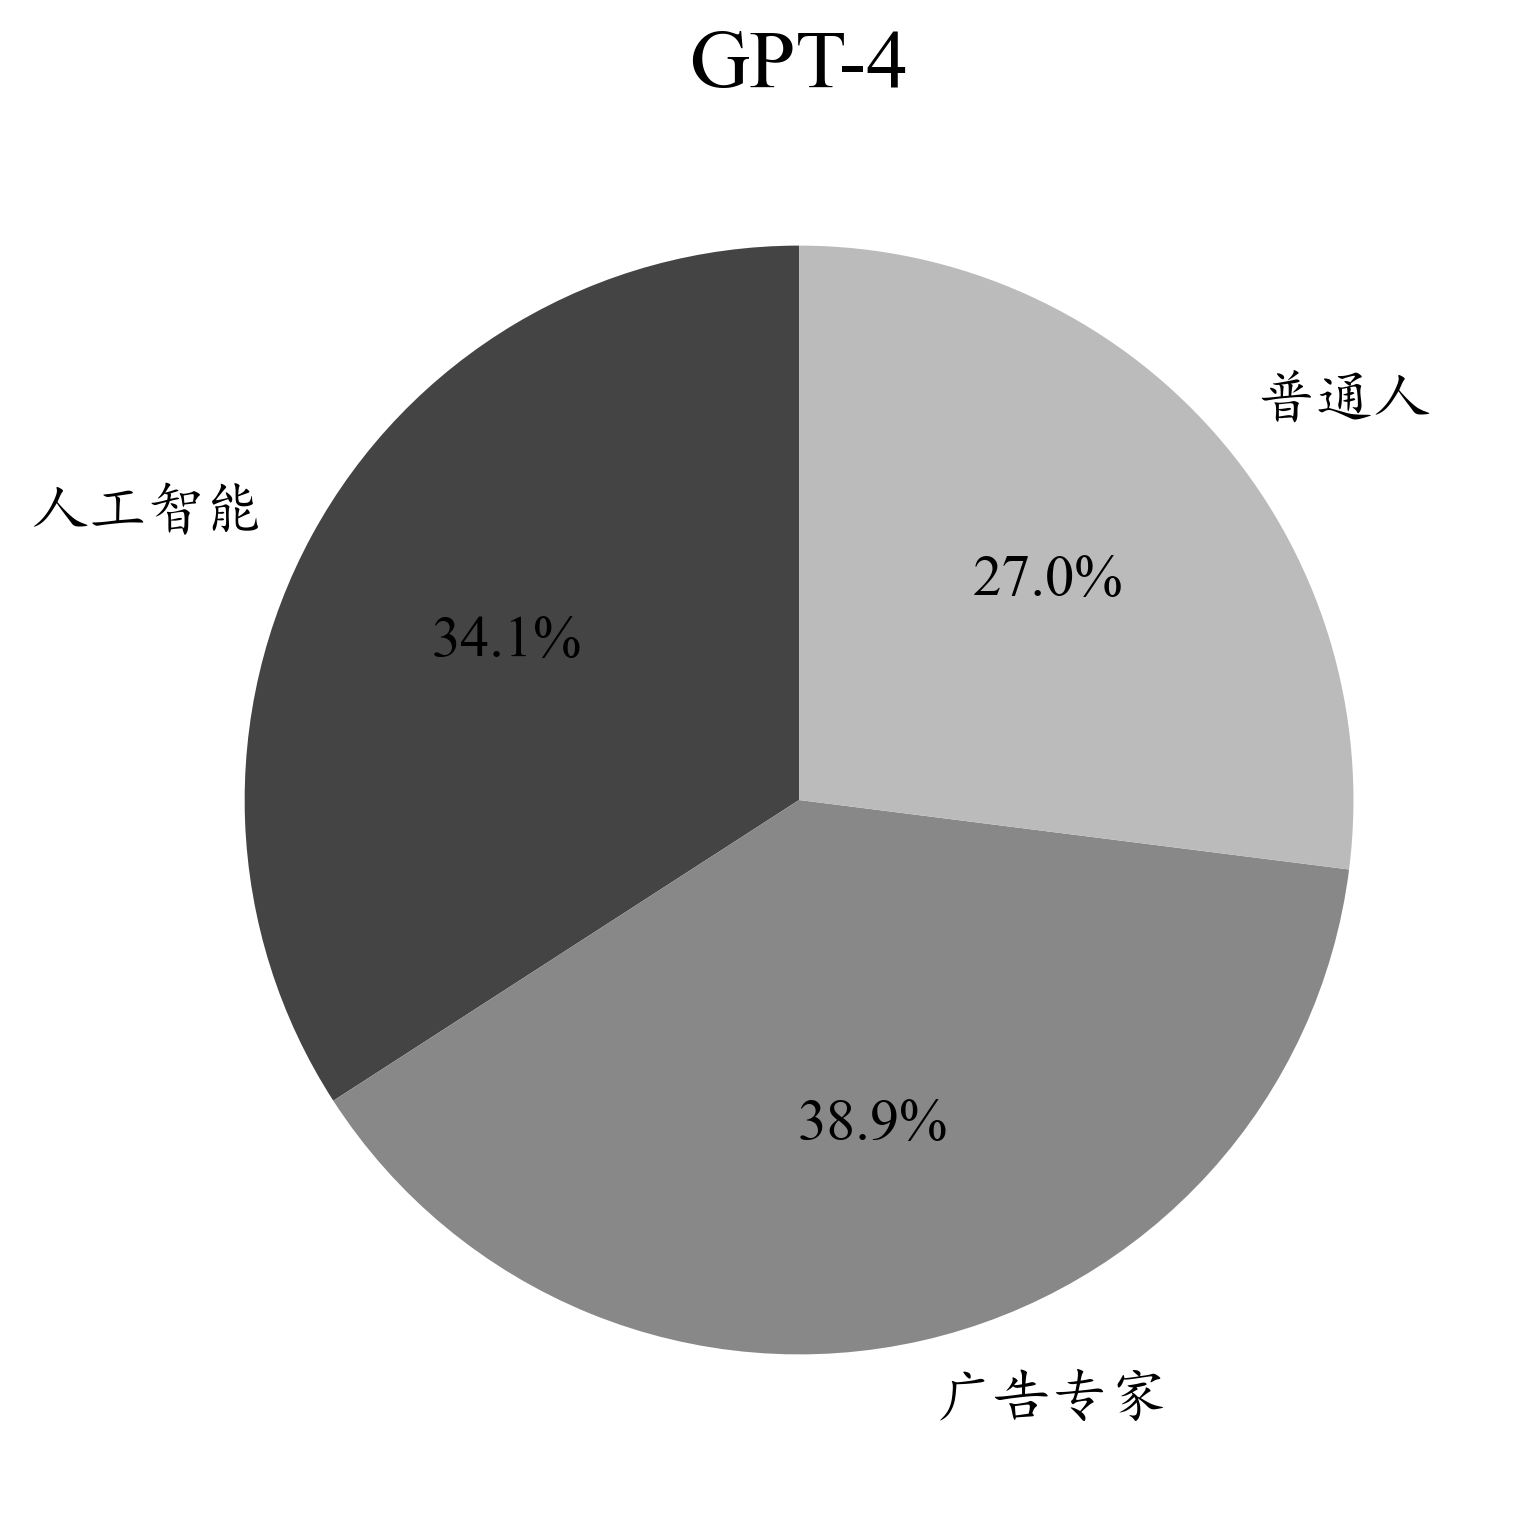
\includegraphics[width=0.4\linewidth]{Image/Study4-exp1-GPT创作者.png}
    }\hspace{2em} % 控制两张图片之间的水平间距
    \subfloat[人类专家创作者]{
        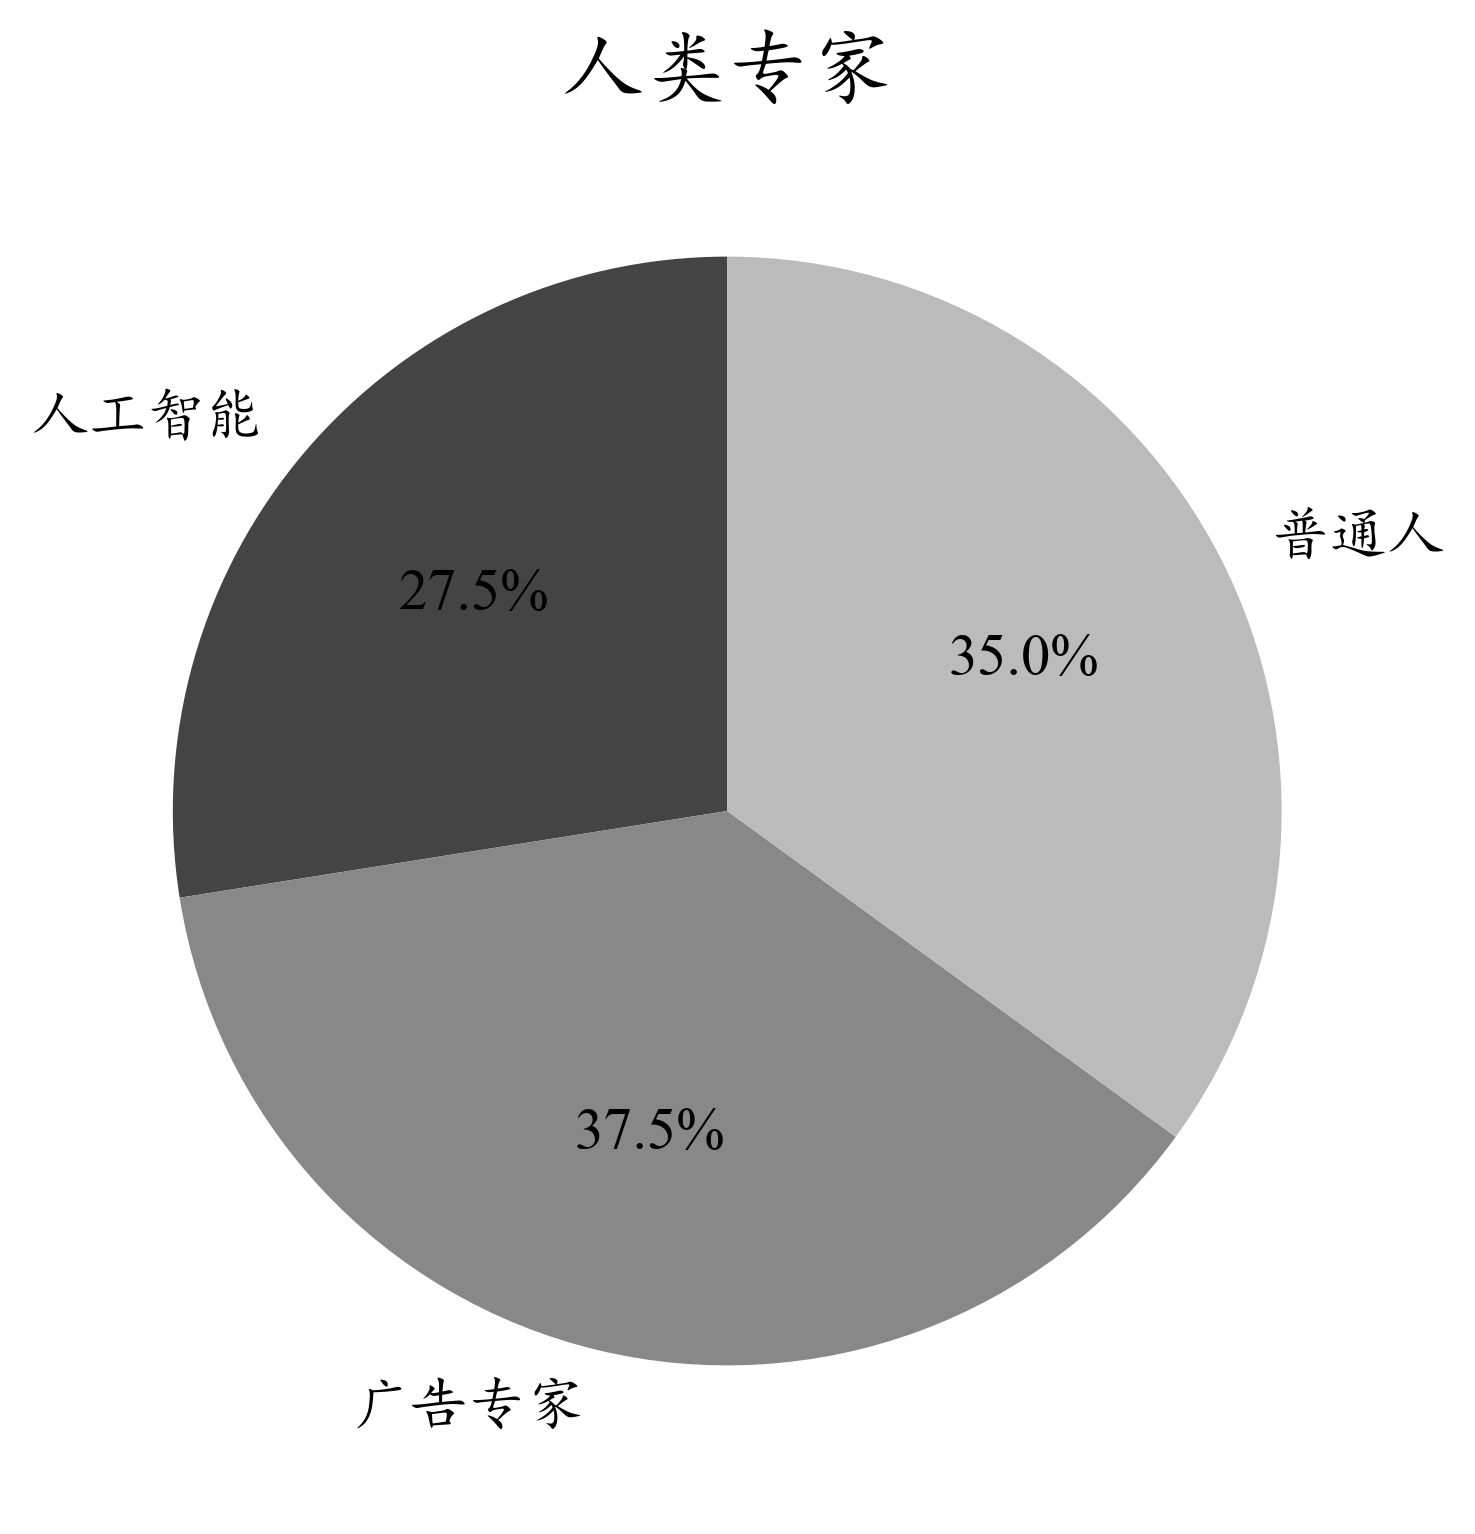
\includegraphics[width=0.4\linewidth]{Image/Study4-exp1-人类专家创作者.png}
    }
    \caption{\label{fig:Study4-exp1-perception} GPT与人类专家实验材料的创作者感知}
\end{figure}

为进一步探讨广告文本的语言特征如何影响受试者对广告来源的推测,本研究基于 LIWC 词法和句法特征进行了单因素方差分析(ANOVA),比较不同广告创作者(AI 生成 vs. 广告专家撰写 vs. 普通人撰写)之间的语言差异。分析结果表明(如表\ref{tab:Study4-substudy1-linguistic_features},不同来源的广告在词汇复杂度、句法结构、指代用法、否定表达、语气表达及冠词使用等方面存在显著差异。

在词汇复杂度方面,AI 生成的广告文本使用了更多的长单词(Sixltr,即包含六个及以上字母的词),其比例最高(0.152),其次是广告专家(0.149),而普通人撰写的广告使用长单词的比例最低(0.033)。这一结果表明,AI 生成的广告语言可能更加正式和专业,而人类撰写的广告更偏向于口语化表达。此外,在句法复杂度方面,AI 生成的广告在句均词数(WPS)上表现出一定优势(22.98),与广告专家(23.31)相近,但均显著高于普通人撰写的广告(22.26)。这表明 AI 生成的广告倾向于使用更长、更复杂的句子,使文本显得更加流畅和结构化,但同时可能降低其口语化程度。

在代词使用方面,AI 生成的广告文本更少使用不定代词(ipron,如“它”“任何”“每个人”),其使用频率最低(1.14),广告专家次之(1.29),而普通人撰写的广告使用最多(1.57)。这一结果可能表明,AI 在生成文本时更注重信息的清晰性,减少了含糊的指代,而人类撰写的广告则更倾向于随意使用不定代词,使文本更具互动感和自然性。此外,在否定表达和比较表达方面,普通人撰写的广告更倾向于使用否定词(negate,如“不会”“没有”),其使用比例最高(1.12),而广告专家使用最少(0.90),AI 生成的广告位于中间(1.21)。相反,AI 生成的广告在比较级(compare,如“更好”“最佳”)的使用频率最高(3.60),其次是广告专家(3.25),而普通人使用最少(3.06)。这一结果表明,AI 生成的广告更倾向于使用比较表达,可能是为了增强广告的说服力,而人类广告撰写者在表达时更直接、更少使用否定表达。

在语气表达方面,AI 生成的广告更倾向于使用推测性语言(discrep,如“应该”“可能”“可以”),其使用比例最高(2.09),普通人次之(1.82),广告专家最低(1.69)。这表明 AI 生成的广告更容易使用可能性或假设性表达,如“你可以实现……”或“这可能会提升你的体验”,而人类广告撰写者更倾向于使用更加确定性的语言,使广告更具信任感。这一结果说明,AI 生成的广告更偏向于正式表达,而人类撰写的广告更倾向于口语化.

最后,在句子结构方面,AI 生成的广告比普通人撰写的广告更频繁地使用前置词(prepend,如“在……之后”“在……之前”),AI 和广告专家的使用比例相同(1.49),均显著高于普通人(1.18)。这表明 AI 生成的广告文本可能更倾向于使用结构更复杂的句式,而人类撰写的广告更偏向简洁直白的表达方式。

综上所述,AI 生成的广告在多个语言维度上表现出与人类撰写广告的显著差异,尤其是在词汇复杂度、句法复杂度、比较表达、推测性语言和句子结构方面更具特点。这些语言特征可能影响受试者对广告来源的判断,使他们更容易将 AI 生成的广告归因于人工智能,而将人类撰写的广告视为人类专家/普通人创作的内容。


\begin{table}[htbp]
    \centering
    \caption{\label{tab:Study4-substudy1-linguistic_features} 语言特征对比}
    {\tablesongti % 整个表格环境应用宋体六号字体
    \renewcommand{\arraystretch}{1.5} % 调整行距
    \begin{tabular}{l c c c c} % 使用 l 让第一列自动调整
        \toprule
        \textbf{语言特征} & \textbf{\( p \) 值}& \textbf{人工智能} & \textbf{广告专家} & \textbf{普通人} \\
        \midrule
        Sixltr & 0.0004 & 0.1523 & 0.1490 & 0.0329 \\
        WPS & 0.0135 & 22.9795 & 23.3107 & 22.2591 \\
        ipron & 0.0079 & 1.1374 & 1.2979 & 1.5702 \\
        negate & 0.0349 & 1.2136 & 0.9048 & 1.1243 \\
        compare & 0.0288 & 3.6045 & 3.2537 & 3.0647 \\
        discrep & 0.0371 & 2.0909 & 1.6954 & 1.8252 \\
        specart & 0.0421 & 2.2395 & 2.2705 & 1.8440 \\
        prepend & 0.0126 & 1.4974 & 1.4973 & 1.1778 \\
        \bottomrule
    \end{tabular}
    }
\end{table}





\section{实验2:AI标签对个性化广告效果的影响}
实验1的结果表明,即使在未明确告知广告来源的情况下,参与者仍能够在一定程度上区分AI生成和人类创作的广告。这表明AI生成广告在语言特征或表达方式上具有独特之处,使其与人类创作的广告有所不同。然而,消费者不仅会根据广告文本的语言特征来推测广告的来源,还可能受到明示信息的影响。当广告明确标注为“AI生成”时,这一信息是否会进一步影响消费者对广告的感知和接受度?换言之,AI 作为广告的生成者,是否会影响个性化广告的说服力?这一问题尚未得到充分探讨。

个性化广告的有效性依赖于心理契合度(psychological fit),即消费者是否认为广告内容与自身需求高度相关。在这一过程中,感知相似性(perceived similarity) 是个性化广告影响消费者态度的核心心理机制 \citep{teeny2021review}。然而,现有研究较少直接测量感知相似性在个性化广告说服过程中的作用,因此本研究首先验证该变量是否确实在个性化广告与消费者态度之间起中介作用。另一方面,人工智能(AI)因缺乏社交属性,往往被认为是心理距离(psychological distance) 更远的主体\citep{kim2020artificial}。心理距离的增加可能导致消费者AI生成广告的感知相似性降低,从而影响个性化广告的说服效果 \citep{ahn2021ai}。换言之,即便AI生成的广告内容符合消费者特征,其个性化效果仍可能因信息来源的影响而受到削弱。基于此,实验2采用两步研究设计,首先验证感知相似性在个性化广告中的关键作用(实验 2a)。实验 2b 在实验 2a 的基础上,进一步引入 AI 标签,以探讨广告来源(AI 生成 vs. 人类创作)是否会影响个性化广告的效果。

\subsection{实验2a:感知相似性的中介探究}
\subsubsection{方法}
(1)被试

实验通过见数平台发布,共 162 名参与者 自愿参加本研究。其中,19 名参与者因未通过注意力检测被剔除,最终保留 143 名有效被试(年龄范围 = 18-48 岁,\textit{M} = 23.83 岁,\textit{SD} = 4.25),其中女性 96 名。每名受试者在完成实验后获得 2 元人民币 作为报酬。

(2)实验材料

本实验采用研究一实验2中的实验材料(\ref{study1-substudy2-methods}),涉及两类产品(薯片与电脑),分别针对尽责性与开放性两个人格特质进行个性化广告设计。对于每种产品-人格特质的组合,实验材料均包含:中性广告(来自社交媒体的原始广告,不包含特定个性化元素);个性化广告(基于该中性广告生成的针对性广告内容,以匹配目标人格特质)。每位参与者需依次观看四组广告(即两种产品 × 两种人格特质),其中每组包含一则中性广告和一则个性化广告。广告呈现顺序随机。观看后,参与者需对每组广告进行评价。

(3)问卷测量

大五人格量表和广告说服效果,测量方法与研究一实验2一致(\ref{study1-substudy2-methods})。除此以外,本实验引入感知相似性 \ref{li2016does},参与者需对以下条目进行评分:“广告的内容符合我的兴趣和需求”,“广告看起来是否像是特地为我设计的”,“广告是否呈现了与我的个性特征相匹配的信息。” 所有测量均采用likert-7点量表(1=完全不同意,7=完全同意),以评估参与者对个性化广告的感知相似程度。

\subsubsection{结果}

在研究一实验2的个性化广告有效的基础上,本实验主要关注感知相似性的中介作用。具体而言,采用 SPSS PROCESS Macro(Model 4) 进行中介效应分析。其中,自变量分别为开放性得分和尽责性得分,因变量为对应个性化广告的说服效果(即开放性个性化广告的效果和尽责性个性化广告的效果),中介变量为感知相似性。

首先,针对开放性维度设计的个性化广告场景(如图\ref{fig:openness-mediation_model}),结果表明开放性得分显著正向预测感知相似性(\textit{b} = 0.8091, \textit{SE} = 0.0892, \textit{t} = 9.0705, \textit{p} < .001),说明高开放性个体更倾向于认为开放性个性化广告符合自身需求。其次,感知相似性显著正向预测广告的说服效果(\textit{b} = 0.5070, \textit{SE} = 0.0335, \textit{t} = 15.1340, \textit{p} < .001)。此外,在控制感知相似性后,开放性得分对广告说服效果的直接效应仍显著(\textit{b} = 0.1289, \textit{SE} = 0.0573, \textit{t} = 2.2482, \textit{p} = .0253)。中介效应分析表明,感知相似性的间接效应为 0.4102,其 95\% 置信区间为 [0.3143, 0.5141],不包含 0,表明感知相似性在开放性个性化广告的个性化效果中起到了中介作用。

\begin{figure}[H] % htbp 让 LaTeX 决定合适的位置
    \centering
    \begin{tikzpicture}[
        node distance=3.5cm,
        every node/.style={align=center, minimum height=1cm, font=\small}, 
        every path/.style={draw, -{Latex[round]}, thick}
    ]
        % 定义变量节点
        \node[draw, rounded corners] (X) {开放性 \\ (自变量)};
        \node[draw, rounded corners, above=of X, xshift=5cm] (M) {感知相似性 \\ (中介变量)};
        \node[draw, rounded corners, right=of X, xshift=5cm] (Y) {个性化说服效果 \\ (因变量)};
        
        % 画箭头,并直接在线上标注路径系数
        \path (X) -- node[midway, above, sloped] {\( 0.8091^{***} \)} (M);
        \path (M) -- node[midway, above, sloped] {\( 0.5070^{***} \)} (Y);
        \path (X) -- node[midway, below, sloped] {\( 0.1289^{*}, 95\% CI=[0.0160, 0.2418] \)} (Y);
        
        % 间接效应标注
        \node[above=0.2cm of M, align=center, font=\small] {
            \textbf{间接效应}: 0.4142, 95\% CI=[0.3143, 0.5141]
        };
        
    \end{tikzpicture}
    \caption{开放性-中介效应模型示意图}
    \label{fig:openness-mediation_model} % 交叉引用时使用 \ref{fig:mediation_model}
\end{figure}

类似地,在针对尽责性维度设计的个性化广告场景中(如图\ref{fig:conscientiousness-mediation_model}),尽责性得分同样显著正向预测感知相似性(\textit{b} = 0.4918, \textit{SE} = 0.0720, \textit{t} = 6.8338, \textit{p} < .001),说明高尽责性个体更倾向于认为尽责性个性化广告符合自身需求。同样,感知相似性显著正向预测广告的说服效果(\textit{b} = 0.4984, \textit{SE} = 0.0298, \textit{t} = 16.7066, \textit{p} < .001)。在控制感知相似性后,尽责性得分对广告说服效果的直接效应仍显著(\textit{b} = 0.1015, \textit{SE} = 0.0392, \textit{t} = 2.5906, \textit{p} = .0101)。中介效应分析表明,感知相似性的间接效应为 0.2451,其 95\% 置信区间为 [0.1566, 0.3388],不包含 0,说明感知相似性在尽责性个性化广告的个性化效果中同样起到了部分中介作用。

\begin{figure}[H] % htbp 让 LaTeX 决定合适的位置
    \centering
    \begin{tikzpicture}[
        node distance=3.5cm,
        every node/.style={align=center, minimum height=1cm, font=\small}, 
        every path/.style={draw, -{Latex[round]}, thick}
    ]
        % 定义变量节点
        \node[draw, rounded corners] (X) {尽责性 \\ (自变量)};
        \node[draw, rounded corners, above=of X, xshift=5cm] (M) {感知相似性 \\ (中介变量)};
        \node[draw, rounded corners, right=of X, xshift=5cm] (Y) {个性化说服效果 \\ (因变量)};
        
        % 画箭头,并直接在线上标注路径系数
        \path (X) -- node[midway, above, sloped] {\( 0.4918^{***} \)} (M);
        \path (M) -- node[midway, above, sloped] {\( 0.4984^{***} \)} (Y);
        \path (X) -- node[midway, below, sloped] {\( 0.1015^{*}, 95\% CI=[0.0244, 0.1785] \)} (Y);
        
        % 间接效应标注
        \node[above=0.2cm of M, align=center, font=\small] {
            \textbf{间接效应}: 0.2351, 95\% CI=[0.1566, 0.3388]
        };
        
    \end{tikzpicture}
    \caption{尽责性-中介效应模型示意图}
    \label{fig:conscientiousness-mediation_model} % 交叉引用时使用 \ref{fig:mediation_model}
\end{figure}


上述分析表明,感知相似性在个性化广告的说服效果中起到了显著的中介作用。即,高开放性/高尽责性的个体在观看与其人格特质匹配的个性化广告时,更倾向于认为广告和自己的相似性,从而增强广告的说服力。此结果验证了感知相似性是个性化广告有效性的关键心理机制,为后续探讨 AI 作为广告生成者是否会影响该机制提供了理论基础。

\subsection{实验2b:AI标签影响的实证研究}
\subsubsection{方法}

本实验采用 $2 \times 2$ 的混合实验设计,其中广告创作者(GPT-4 vs. 人类专家)作为被试间变量,个性化程度(个性化 vs. 非个性化)作为被试内变量。实验旨在探讨 AI 作为广告创作者是否会影响个性化广告的说服效果,并考察个性化广告与信息来源之间的交互作用。


(1)被试

实验通过见数平台发布,共304名参与者自愿参加研究。经注意力检测筛选后,共剔除16名不合格的参与者,最终纳入288名有效被试(年龄范围 = 20-69岁,$\textit{M} = 31.45$,$\textit{SD} = 9.27$),其中146名为女性。所有被试在完成实验后均获得2元人民币作为报酬。

(2)实验材料

本实验选取小米手机(广告中匿名为「M手机」) 在社交媒体上的真实广告文本,并基于该广告文本指导GPT-4生成个性化版本。生成后确保所有广告文本具有相同的产品信息。采用的提示词(prompt)是:“请根据下面的社交媒体上的中性广告内容,修改为两个版本的个性化广告文案,使得目标消费者购买意愿增强,尽管其他消费者不一定喜欢:
1. 针对高外倾性消费者的版本。
2. 针对低外倾性消费者的版本。”

(3)实验流程

在阅读广告材料之前,所有参与者都会根据自己所分配到的条件,被告知特定的广告创造者(cover story)。如果参与者被分配到GPT-4,对广告创作者的描述为:“M手机是一款即将推向市场的智能手机。在本研究中,我们希望了解您对两段广告文案的反馈,以便根据用户反馈优化广告设计。您即将看到的广告文案是由 GPT-4 生成的。GPT-4 是 OpenAI 开发的一款先进的人工智能模型,专门用于理解和生成文本。” 如果参与者被分配到人类专家组,对广告创作者的描述则为:“M 手机是一款即将推向市场的智能手机。在本研究中,我们希望了解您对两段广告文案的反馈,以便根据用户反馈优化广告设计。您即将看到的广告文案是由经验丰富的市场营销专家撰写的,他们擅长创意广告设计和理解消费者心理。” 接下来,所有被试需阅读两则广告文案(一则为针对高外倾设计的广告,一则为低外倾设计的广告),广告呈现顺序随机。参与者需在阅读完每则广告后,完成问卷效果的测量,两则广告评价完后完成人格量表和性别、年龄等人口统计学信息。

(4)问卷测量

a. 说服效果。采用研究一实验2的测量方法(\ref{study1-substudy2-methods})。被试需对广告的说服力进行评分,共包含 5 个题目,采用 1-5 点李克特量表 评分,最终计算平均值作为说服效果得分。

b. 外倾性人格量表:本实验关注外倾性这一人格特质,因此从 \citet{john1991big} 编制的 大五人格量表(BFI-44) 中筛选与外倾性相关的 8 道题目,要求被试根据自身情况进行评分(1=完全不符合,5=完全符合)。

\subsubsection{结果}
首先,为计算个性化水平,本研究以被试的外倾性得分中位数为划分标准,将外倾性得分大于或等于中位数的被试归类为高外倾群体,低于中位数的被试归类为低外倾群体。在广告呈现方面,对于高外倾个体而言,观看专门针对高外倾性设计的广告被定义为个性化广告,而观看针对低外倾性设计的广告则被定义为非个性化广告。相应地,对于低外倾个体而言,观看针对低外倾性设计的广告被定义为个性化广告,而观看针对高外倾性设计的广告则被定义为非个性化广告。

为了探讨广告创作者标签(GPT-4 vs. 人类专家)对个性化广告说服效果的影响,本研究采用了 $2 \times 2$ 的重复测量方差分析,其中个性化(个性化 vs. 非个性化)作为被试内变量,广告创作者标签(GPT-4 vs. 人类专家)作为被试间变量。结果表明(如图\ref{fig:Source_personalization}),个性化与广告创作者标签之间的交互作用达到显著水平,$\textit{F}(1,112) = 6.866, \textit{p} = .010, \eta_p^2 = .058$,表明个性化广告的效果受到广告创作者标签的影响,即标注不同来源的广告在个性化说服力上的表现存在显著差异。进一步的简单效应分析显示,在被标注为人类专家创作的广告中,个性化广告的说服力显著高于非个性化广告(均值差异 = -0.171, 标准误 = 0.092, $\textit{p} = .028$,95\% CI = [0.010, 0.035]),说明当广告被标注为由人类专家撰写时,个性化广告的优势得以体现,受众更容易接受个性化内容。然而,在被标注为 GPT-4 生成的广告中,个性化广告与非个性化广告的说服力差异并不显著(均值差异 = 0.166, 标准误 = 0.090, $\textit{p} = .102$,95\% CI = [-0.023, 0.344]),说明当广告明确标注为 AI 生成时,个性化广告的优势效应被削弱。这一结果表明,即使广告文本内容完全相同,仅仅是信息来源的标注差异,就足以影响个性化广告的说服效果,进一步验证了AI作为信息源在个性化广告中的重要影响。

\begin{figure}[H]
    \centering
    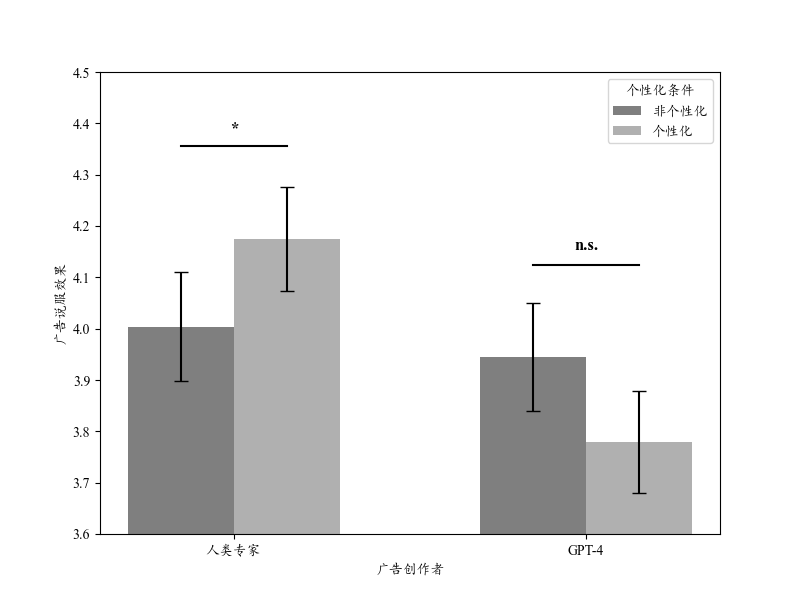
\includegraphics[width=1\linewidth]{Image/Study4-Source_Personalization.png}
    \caption{\label{fig:Source_personalization}广告创作者对个性化广告说服力的影响}
\end{figure}
\section{讨论}

本研究探讨了AI作为个性化广告信息源时对个性化广告效果的影响,并揭示了信息来源在个性化广告的说服过程中所起的关键作用。研究结果表明,个性化广告的有效性受到感知相似性的中介作用,即当受众认为广告内容与自身特质相匹配时,其说服效果更强 \citep{li2016does, teeny2021review}。然而,当 AI 作为广告创作者的身份被明确标注 时,即使广告文本本身符合目标受众的人格特质,其说服力仍然受到削弱。这一发现表明,个性化广告的有效性不仅取决于内容本身,还受到受众对信息来源的认知影响。

在 信息来源认知 方面,研究结果显示,在信息来源未知的情况下,受众能够基于文本特征推测广告创作者,并且 AI 生成的广告在语言风格上与人类专家撰写的广告表现出系统性差异。然而,当信息来源被明确标注为 AI 时,个性化广告的说服力下降,受众对广告的信任度也随之降低。这一现象可以通过 感知相似性在个性化广告中的中介作用 来解释。AI 作为信息源会增加受众与广告之间的心理距离 \citep{kim2020artificial, ahn2021ai},导致受众在认知上将 AI 视为一个较远的主体,从而降低他们与广告的心理契合度,并最终削弱个性化广告的整体效果。

这一发现对 AI 生成个性化广告的优化策略 具有重要启示。首先,AI 生成广告的优化不应仅停留在匹配目标人格特质的语言风格,而应进一步增强广告的“人性化”表达,以提升其交互性和情感共鸣。例如,研究表明,使用第一人称(I/we)和直接面向受众的语言(you)能够增强个性化体验,减少 AI 生成广告与受众之间的心理距离 \citep{markowitz2020communicating}。这种语言策略能够让广告显得更具互动性,使受众更容易产生自我联结,进而提升个性化广告的说服力。

其次,在 AI 生成广告的披露策略 上,应探索 降低 AI 作为信息来源可能带来的负面影响。研究发现,当 AI 生成的内容被描述为“结合专家意见”或“基于大数据精准分析”时,其可信度和接受度会有所提升 \citep{puerta2022human}。因此,在政策可能要求 AI 生成广告必须披露信息来源 的情况下,企业可以调整披露方式,例如 强调 AI 在广告创作中的辅助角色,而非主要创作者,或通过 人机共创(human-in-the-loop)模式 让人类专家优化 AI 生成的广告内容。这一策略不仅可以结合 AI 的 高效性和大规模数据处理能力,还能够 保留人类专家的创造力和情感共鸣能力,使 AI 生成的个性化广告在 提高传播效率的同时,仍然具备较强的个性化吸引力。


\chapter{总讨论}
近年来,生成式人工智能(Generative AI),尤其是 大语言模型(Large Language Models, LLMs),在文本生成领域展现出巨大的潜力。AI 不仅具备自主生成信息(如广告文本)的能力 \citep[例如][]{karinshak2023working, bai2023artificial},还能够根据目标受众的特征快速调整广告风格,从而增强个性化匹配度 \citep[例如][]{matz2024potential, simchon2024persuasive}。这一特性使得 AI 在个性化广告创作中展现出广阔的应用前景,然而,其生成的个性化广告是否真正有效仍需进一步验证。一方面目前尚不清楚 AI 是否能针对不同人格特质、不同匹配水平、不同生成方式,稳定地生成有效的个性化广告。另一方面,人们是否能区分 AI 与人类专家撰写的广告?如果 AI 的身份被明确告知,这种信息来源的认知是否会影响个性化广告的接受度?这些问题在现有研究中尚缺乏系统性的探讨。基于此,本研究围绕这些核心问题展开,采用四个子研究,系统性地探讨 AI 生成的个性化广告的有效性、适用性以及优化路径。

子研究 1 旨在验证 AI 生成个性化广告的有效性及其在人格匹配上的适应性。通过多个实验,本研究首先采用 GPT 生成针对大五人格不同特质的个性化广告,并评估其在不同人格特质群体中的说服效果。结果表明,AI 生成的个性化广告在 外倾性和宜人性群体 中表现出较强的匹配效应,而在 尽责性和神经质群体 中,匹配效应较为不稳定。此外,GPT-4 在个性化广告生成上的表现优于 GPT-3.5,尤其在 开放性和尽责性群体 中,其广告匹配度显著提高。进一步的实验探讨了 AI 在不同广告创作情境下的表现,发现 AI 不仅能够从零生成个性化广告,还能够基于现有广告文本进行个性化改写,表明其在个性化广告定制中的灵活性。

子研究 2 进一步比较了 AI 与人类专家在个性化广告创作中的差异,并探讨 AI 优化人类专家广告文本 的潜力。实验结果表明,AI 在多个特质(如尽责性)上的个性化效果甚至优于人类专家,但在人类创作较具优势的 宜人性广告 维度上,AI 仍存在一定局限。然而,当 AI 用于优化人类专家撰写的广告 时,其个性化广告的效果在宜人性维度上显著提升,这表明 AI 不仅能够独立生成个性化广告,还能够增强人类专家创作的广告的个性化匹配度。

子研究 3 采用文本分析与预测建模的方法,深入探讨 AI 生成的个性化广告文本与实际受众广告偏好之间的匹配性。通过对不同人格特质个性化广告的语言特征进行分析,研究发现,AI 生成的广告语言风格在大多数情况下能够与目标人格特质相匹配,但在特定特质(如神经质和低开放性个体)上,其语言风格匹配度较低,且在尽责性维度上出现 负向匹配效应,即高尽责性个体更偏好针对低尽责性设计的广告,低尽责性个体则更倾向于高尽责性广告。此外,研究发现 个性化广告的语言特征匹配与个体实际广告偏好之间并非完全一致,AI 生成的个性化广告在某些情境下可能过于依赖人格特质的表层语言风格,而忽略了目标受众在广告语境下的更深层次的需求偏好。

子研究 4 进一步探讨了 AI 作为信息源对个性化广告接受度的影响,重点考察 当受众知道广告由 AI 生成时,其对广告的态度是否发生变化。研究结果表明,受众能够基于语言风格判断广告创作者,但当 AI 作为广告创作者的身份被明确披露 时,个性化广告的说服力下降。这一现象表明,个性化广告的接受度不仅取决于广告内容本身,还受到受众对信息来源的认知影响。AI 作为信息源可能 增加受众与广告之间的心理距离,从而降低个性化广告的契合度,特别是在需要情感共鸣的广告类型中,AI 生成的广告可能因缺乏人类创作者的情感深度而影响受众的信任度。这一发现提示,在实际应用中,AI 生成的个性化广告需要在信息来源披露方式上进行优化,以减少 AI 作为广告创作者的潜在负面影响。

综合来看,本研究通过 四个子研究,系统性地探讨了 AI 生成的个性化广告的有效性、AI 在个性化匹配上的优势与局限、AI 生成广告文本的语言风格与实际受众偏好的匹配度,以及 AI 作为信息源对个性化广告说服力的影响。研究结果不仅验证了 AI 在个性化广告创作中的应用潜力,也揭示了 AI 在不同人格特质群体中的适应性差异,并提供了 优化 AI 生成广告内容及披露策略 的方向。

\section{AI生成的个性化广告的有效性及其局限}

本研究的结果表明,AI 生成的个性化广告在一定程度上展现出较强的说服力,但其有效性并不均衡,受不同人格特质、匹配水平和广告创作方式的影响。研究发现,AI 在外倾性和开放性个体中能够稳定生成符合受众偏好的广告,而在宜人性、尽责性和神经质个体中,其匹配效果较为不稳定,甚至在某些情况下完全失效。此外,AI 生成的广告在语言风格匹配上虽然能够与目标受众保持一致,但在实际广告偏好和说服力上,仍然存在一定的局限性。

首先,\textbf{AI 在不同人格特质群体中的有效性存在差异}。研究一的结果表明,开放性和外倾性是两个较为稳定的人格维度,无论是高水平还是低水平个体,AI 都能够生成符合其偏好的个性化广告文本,并在匹配度和说服效果上表现出显著优势。相比之下,宜人性和尽责性的个性化广告效果则较为不稳定。宜人性的高水平个体始终能够被有效匹配,而低水平个体的匹配效果取决于广告生成方式:在基于中性广告改编的条件下,AI 仍能生成有效的个性化广告,但在基于产品描述直接生成的条件下,个性化效果未能显现。尽责性个体则表现出相反的趋势,高尽责性个体能够被 AI 生成的广告有效匹配,而低尽责性个体始终未能在任何条件下展现出显著的匹配效应。此外,神经质是唯一一个在所有条件下均未能展现个性化匹配效应的人格维度,无论是高水平还是低水平个体,AI 生成的个性化广告在该维度上的效果均不显著。这些发现表明,AI 在生成个性化广告时,并非对所有人格特质均能实现稳定的匹配效果,不同人格特质的个性化适配性可能受到目标受众的特质特征、广告生成方式以及个性化策略本身的影响 \citep{winter2021effects}。进一步地,研究二的结果表明,AI 与人类专家在个性化广告创作中的表现亦存在显著差异。在尽责性广告的个性化匹配度上,AI 的表现甚至优于人类专家,而在人类更具优势的宜人性广告维度上,AI 仍然存在一定局限。这一发现表明,AI 在处理结构化、目标导向型的信息(如尽责性广告)时可能更具一致性,而在人类专家擅长的情感共鸣和社交互动类广告(如宜人性广告)中,AI 的表达方式相对较为刻板,缺乏人类创作者所具备的情感深度。此外,研究进一步发现,当 AI 用于优化人类专家创作的广告文本时,其个性化广告的整体说服效果在宜人性维度上得到了显著提升。这表明 AI 并非单纯地替代人类创作者,而是具备增强人类专家广告个性化表达的潜力。在实际应用中,这一结果提示,AI 生成的个性化广告可以作为辅助工具,与人类创作者协同工作 \citep{yoon2024designing},以结合 AI 的高效性和人类创作者的情感共鸣能力,从而优化个性化广告的整体表现。

其次,\textbf{AI 生成的个性化广告在不同人格特质上的匹配效果存在局限性,主要体现在其对受众需求的理解较为表层化,未能充分结合广告语境中的深层次偏好。}研究三通过文本分析和预测建模,系统性比较了 AI 生成的个性化广告与用户的实际广告偏好,发现尽管 AI 能够在语言风格上模仿不同人格特质的表达方式,但其个性化策略往往停留在表层特征,而未能深入把握广告情境下受众的信息加工方式。例如,高开放性个体在日常交流中更倾向于使用抽象、探索性的语言风格,因此 AI 在生成个性化广告时,往往更关注这类语言特征的匹配。然而,在广告语境中,由于广告本质上是一种说服性传播,高开放性个体在深层加工过程中可能更关注因果逻辑与创新创意的结合,而非单纯的发散思维和抽象表达。换言之,AI 可能能够识别并复制开放性个体在一般语境中的语言风格,但在个性化广告场景下,其生成的内容未能充分结合广告的传播目标,导致个性化匹配的有效性受限。同样,宜人性个体的广告偏好在过往研究中未得到充分探讨,既有文献通常强调宜人性个体偏好和谐、温暖的沟通方式。然而,研究三的结果表明,高宜人性个体不仅关注广告的社交取向,还关注广告如何凸显产品在人际关系或个人体验中的独特性。例如,他们可能更倾向于看到产品如何促进人与人之间的联系,或如何体现个体在社群中的积极形象,而 AI 生成的个性化广告往往只是简单地强调情感共鸣,忽略了这些更深层次的社交价值表达。低宜人性个体则倾向于直接、批判性更强的广告风格,而 AI 生成的广告通常采用更温和、含蓄的表达方式,导致个性化匹配的有效性下降。此外,在神经质维度上,研究三的结果揭示了高神经质与低神经质个体在广告偏好上的表现形式相似但驱动因素不同。高神经质个体关注情绪共鸣,但更需要即时的情绪安抚,如非正式表达和即时满足;相比之下,低神经质个体对情绪化广告内容的接受度较高,但更偏好结构清晰、强调事实与稳定性的广告信息。这一发现表明,神经质个体的个性化广告设计不能仅依据其在日常语言中的情绪表达特征,而应结合个体在广告语境下的实际心理需求进行优化。

综上所述,AI 生成的个性化广告在不同人格特质群体、不同广告创作方式和不同语言风格适配度上,均展现出一定的有效性,但也存在局限性。研究一和研究二的结果表明,AI 在某些人格特质(如外倾性和宜人性)群体中能够有效地提升广告说服力,但在尽责性和神经质群体中,其匹配效应存在不稳定性。此外,研究三的文本分析进一步揭示了 AI 生成广告的语言风格与实际广告偏好的不完全一致性,说明个性化广告的优化需要超越语言特征匹配,进一步结合目标受众在广告语境下的认知方式、信息加工需求和心理调节机制。研究二的实验也表明,AI 生成广告在某些情况下可以有效地优化人类专家创作的广告文本,特别是在需要结构化、逻辑清晰的信息表达时,AI 可能更具优势,而在人类创作者更具情感表达能力的广告(如宜人性广告)中,AI 仍然面临一定的挑战。这些发现共同表明,AI 生成的个性化广告的有效性虽然得到了一定验证,但其适用性并非普适,未来的优化方向应结合认知科学与广告传播的多维视角,使个性化广告不仅能够匹配目标人格特质的语言风格,更能精准满足不同群体的实际广告接受模式。

\section{AI作为信息源对个性化广告的影响}
本研究进一步探讨了 AI 作为信息源对个性化广告接受度的影响。尽管 AI 在个性化广告创作中展现出一定的有效性,但广告的说服力不仅依赖于内容本身,也受到信息来源的影响。研究四的实验结果表明,当受众未知广告创作者身份时,他们能够基于语言风格对广告的来源做出一定推测,但这种判断并不总是准确,因此不会直接影响广告的说服力(研究二)。然而,当 AI 作为广告创作者的身份被明确披露后,受众对个性化广告的接受度整体下降,广告的说服力随之削弱,受众的信任度也降低。这一现象表明,个性化广告的有效性不仅取决于广告内容本身,还受到受众对 AI 作为信息源的认知影响。


\textbf{当广告来源未知时,受众可以在一定程度上区分 AI 生成的广告与人类专家撰写的广告,但这种区分能力并不稳定。}具体而言,GPT 生成的广告更倾向于被识别为 AI 生成的,而人类创作的广告更倾向于被认为是由人类撰写的。然而,实验结果也显示,部分 AI 生成的广告会被误认为是人类创作的,而部分人类创作的广告可能被误认为是 AI 生成的 \citep{chaka2024reviewing}。这一现象表明,受众对 AI 生成广告的辨别能力并不完全可靠,同时也反映了 AI 在某些情境下能够较好地模拟人类表达,使广告信息的来源变得模糊。这一发现强调了信息来源披露可能带来的影响,并提示未来在 AI 生成广告的实际应用中,需要更加谨慎地制定信息披露策略。此外,本研究的实验验证了感知相似性在个性化广告接受度中的作用。实验结果表明,当广告内容与受众的人格特质匹配时,受众对广告的感知相似性更高,进而增强广告的接受度。结合这一发现,本研究进一步探讨了 AI 作为信息来源的披露如何影响广告接受度,\textbf{并假设当 AI 作为广告创作者的身份被明确披露后,受众可能会认为 AI 并不能真正理解个体需求,从而增加受众与广告之间的心理距离\citep{kim2020artificial, ahn2021ai},进而削弱广告的整体说服力。}这一发现表明,在个性化广告的应用中,AI 生成的广告不仅需要语言风格的匹配,还需要综合考虑信息来源的影响,以降低 AI 作为广告创作者可能带来的负面效应。


这一发现对 AI 生成个性化广告的优化策略具有重要启示。一方面,优化 AI 生成广告的表达方式 可以减少受众对 AI 作为信息源的心理距离,从而提高广告的接受度。研究表明,使用第一人称和直接面向受众的语言能够增强个性化体验,使广告更加具有互动性,并提升其说服力 \citep{markowitz2020communicating}。此外,在强调情感共鸣和社交互动的广告类别中,AI 生成的文本可以融入更多自然的人类表达方式,例如加强幽默、情感化描述和叙述性元素,以降低 AI 生成文本的刻板印象,使其更符合人类创作的风格。研究二的对比实验表明,AI 在尽责性广告的个性化匹配上展现出较强的逻辑性和信息密度,比人类专家创作的广告更具说服力;而在宜人性广告维度上,GPT-4 通过优化人类专家撰写的广告文本,使个性化效果显著提升。这一结果表明,AI 生成的个性化广告不仅可以通过调整语言策略增强自身的接受度,同时也可以通过与人类专家的结合,进一步提升广告的个性化适配性。另一方面,调整 AI 生成广告的信息披露方式 也可以有效降低 AI 作为信息来源可能带来的负面影响。研究发现,当 AI 生成的内容被描述为“结合专家意见”或“基于大数据精准分析”时,其可信度和接受度有所提升 \citep{puerta2022human}。这表明,即使政策要求披露 AI 生成广告,企业仍可以通过优化披露方式来减少 AI 身份对广告接受度的负面影响。例如,可以在广告中强调 AI 在创作过程中的辅助角色,而非主要创作者,或采用人机共创(human-in-the-loop)模式,让人类专家优化 AI 生成的广告内容。这种方式不仅能够结合 AI 在数据分析和高效文本生成方面的优势,同时也能保留人类专家的创造力和情感共鸣能力,使广告既具备规模化生成的优势,又能保持个性化和真实性。

综上所述,AI 作为信息源对个性化广告的影响具有双重特性。一方面,AI 生成的广告在逻辑性和信息传递方面展现出一定优势,特别是在尽责性和开放性广告类别中,AI 可能比人类专家更具说服力;但另一方面,在强调情感共鸣和社交互动的广告类别中,AI 生成的广告在披露后可能会削弱受众的信任感,导致广告说服力下降。因此,在 AI 生成个性化广告的实际应用中,应综合考虑受众对信息来源的认知影响,优化 AI 生成广告的语言策略,并探索更灵活的信息披露方式,以最大程度地发挥 AI 在个性化广告创作中的优势,同时减少 AI 作为信息源可能带来的消极效应。

\section{个性化广告的优化路径}
本研究的结果表明,AI 生成的个性化广告在一定程度上展现出较强的说服力,但其有效性受多种因素影响,包括目标受众的人格特质、个性化匹配程度、广告创作方式以及信息来源的认知。在此基础上,优化 AI 生成的个性化广告,需要在理论层面进一步明确个性化广告的关键作用机制,并在实践层面结合 AI 提示词优化、信息来源管理及人机共创模式,以提升广告的个性化匹配效果和受众接受度。

在理论层面,本研究的核心贡献体现在个性化广告的匹配机制、AI 与人类专家的互补性以及信息来源认知对广告接受度的影响。首先,\textbf{个性化广告的匹配机制不仅依赖于表层语言风格,而是深层次的信息加工方式决定了个体对广告内容的偏好}。过往研究主要基于大五人格特质设计广告内容,但匹配效应的稳定性存在一定争议 \citep{matz2017psychological,winter2021effects}。本研究通过文本分析和实验发现,个性化广告效果的不稳定性可能源于不同人格特质个体在广告情境下的信息处理方式更具独特性。例如,高开放性个体在日常交流中偏好抽象、探索性的语言风格,AI 生成的广告也能模仿这一特点。然而,在广告语境中,高开放性个体更关注因果逻辑与创新创意的结合,而非单纯的抽象表达。类似地,高神经质个体在一般对话中展现出高情绪性的语言特点,但在广告中,他们更倾向于非正式表达和即时满足,而非强化负面情绪。因此,AI 生成的个性化广告不能仅依赖于语言风格的匹配,而需要进一步结合目标受众在广告情境下的实际信息加工方式。其次,\textbf{信息来源的认知影响也是个性化广告接受度的重要因素。}本研究的实验验证了感知相似性在个性化广告接受度中的中介作用,发现受众更倾向于接受与自身特质相似的信息来源。当广告创作者身份未知时,受众可以在一定程度上推测广告来源,但这种判断并不总是准确,因此对广告接受度的影响有限。然而,当 AI 作为广告创作者的身份被明确披露后,个性化广告的说服力下降。这一现象可能源于 AI 作为信息源所带来的心理距离,使得受众难以产生认同感,从而降低广告的可信度和影响力。特别是在强调情感共鸣的广告(如宜人性广告)中,受众更倾向于相信由人类专家创作的广告,而 AI 生成的广告则可能因缺乏情感真实性而削弱其说服力。此外,本研究还发现\textbf{ AI 与人类专家在个性化广告创作中各有所长,二者在不同广告类别中的优势互补}。在尽责性广告中,AI 生成的广告由于逻辑性强、信息密度高,能够精准匹配目标群体的需求,甚至优于人类专家的创作。然而,在宜人性广告中,人类专家的表达能力更具优势,能够更自然地融入情感共鸣和社交互动的元素,而 AI 生成的广告则可能显得较为刻板。因此,AI 在个性化广告中的最佳角色可能并非完全替代人类创作者,而是作为辅助工具,与人类专家协同工作,以优化广告创作效果。

基于上述理论机制,在实践层面,本研究提出了针对 AI 个性化广告的优化策略,包括优化 AI 语言风格的操控方式、采用人机结合的广告创作模式以及调整 AI 生成广告的披露方式,以提升个性化广告的整体效果。首先,AI 生成的个性化广告在现有实践中主要依赖于提示词优化,但仅关注表层语言风格可能无法达到最佳的说服效果。本研究的发现表明,优化 AI 生成广告的一个关键策略是改进提示词设计,使 AI 在创作过程中不仅关注受众的语言风格,还能结合目标群体的认知偏好。\textbf{进一步的优化手段包括基于少样本学习和微调技术,使 AI 在训练过程中融入更符合个性化广告需求的文本示例。}此外,利用研究三的预测建模方法,可以快速评估 AI 生成广告的有效性,帮助进一步优化提示词或生成模型,以提升广告的匹配度 \citep{raut2023reinforcing}。在人机结合的广告创作模式方面,本研究发现 AI 在情感共鸣较强的广告类别(如宜人性广告)中表现不及人类专家,但当 AI 用于优化人类专家撰写的广告文本时,个性化广告的整体说服效果得到了提升。\textbf{这表明,与其让 AI 独立创作广告,不如让 AI 在已有广告文本的基础上进行优化,以更符合受众的需求}。人机结合的广告创作模式不仅能够提升个性化广告的效果,还能够保留 AI 在高效生成和优化广告方面的优势,同时结合人类创作者的情感共鸣能力,使广告更具吸引力。在 AI 生成广告的披露方式方面,本研究发现,受众在未知广告来源的情况下,对 AI 生成的广告接受度较高,但当 AI 身份被明确披露后,广告的说服力下降。这一结果表明,优化 AI 生成广告的披露方式是降低 AI 负面认知的重要策略。例如,研究发现,当 AI 生成的广告被描述为“结合专家意见”或“基于大数据精准分析”时,其可信度和接受度显著提升。因此,即使政策要求披露 AI 生成广告,企业仍可以通过优化披露方式减少 AI 身份对广告接受度的负面影响。另一种可能的策略是采用人机共创的模式进行披露,即让 AI 生成的广告由人类专家审核和优化,并在披露信息中强调人类专家的参与,从而降低 AI 生成广告带来的心理距离。

总体而言,本研究的发现不仅拓展了 AI 生成个性化广告的理论基础,还为实践中的广告优化提供了可行的策略。从理论层面来看,本研究揭示了个性化广告优化不仅需要语言风格匹配,更需结合受众的深层需求、感知相似性以及 AI 作为信息源的影响。从实践层面来看,本研究提出了基于优化 AI 语言风格、人机结合创作以及调整披露方式的策略,以提升 AI 生成个性化广告的整体效果。未来,随着 AI 在广告行业中的应用不断发展,如何进一步优化 AI 生成的广告内容,使其既能保持高效性,又能增强受众的认同感和信任感,将成为个性化广告研究的重要方向。

\section{研究局限及未来研究方向}

本研究尽管对 AI 生成个性化广告的有效性和适用性进行了系统性探讨,但仍然存在一些值得进一步优化和扩展的局限性。可以从以下几个方面进行梳理:个性化匹配机制的复杂性、数据特征的局限性、广告形式的单一性、因变量的现实贴合度、以及理论基础的进一步拓展。每一方面的局限性不仅影响了当前研究结论的适用性,也为未来研究提供了新的探索方向。

首先,关于大五人格特征的个性化设计,本研究主要基于单一维度进行设计和实验检验。但实际上,个性化广告的有效性可能涉及多个特质的交互作用。在实验过程中,本研究发现,尽管低尽责性个体的个性化广告匹配效果并不稳定,但其偏好词语却展现出高开放性的语言特征。这表明,不同人格特质可能并非完全独立,而是相互影响,并在个性化广告偏好中表现出复杂的交互关系。因此,未来研究可以进一步探讨多个特质的组合如何影响个性化广告的接受度。例如,开放性与尽责性的交互是否会影响信息复杂度的接受度?外倾性与神经质的组合是否会影响情绪导向广告的有效性?这些问题值得在后续研究中进一步挖掘。此外,个性化广告的匹配策略通常基于单一特质的优化,但如果能够将多个特质融合进 AI 的个性化生成机制中,可能会更精准地满足个体的真实需求。未来研究可以尝试构建多维特质的匹配模型,探索如何在 AI 生成广告时,综合考虑个体在多个特质上的表现,以优化广告的说服力和个性化效果。

其次,特征选择上,目前,研究主要依赖于大五人格特质作为个性化广告的匹配维度,而在实际应用中,受众的个性化信息不仅来自于自我报告的人格测量,还可以通过其他行为数据进行建模。例如,社交媒体上的互动模式、历史购物记录、兴趣标签等都可以反映个体的个性特征,甚至在某些情况下,比传统人格测量更具预测力。已有研究尝试利用大五人格特质预测个体的消费偏好和社交媒体行为\citep{kosinski2013private, golbeck2011predicting},那么,未来研究可以进一步探索,AI 是否可以直接基于这些数据进行特征提取和个性化广告生成,而不依赖于传统的人格测量?这不仅可以降低用户数据收集的成本,也可能提升个性化广告的适用性和精准度。此外,AI 生成广告的个性化能力是否可以进一步结合受众的实时行为反馈进行动态优化?例如,AI 是否可以基于用户的实时交互(如点击、浏览时长、互动行为等),持续调整广告的个性化程度,以提高广告的效果?这些问题都值得未来研究深入探讨。

第三,广告形式上,本研究主要关注 AI 在文本广告创作中的个性化能力,而在实际营销环境中,广告通常包含更丰富的形式,如图文广告、短视频广告、甚至虚拟现实(VR)广告等。已有研究表明,视觉元素在个性化广告传播中发挥着至关重要的作用,消费者的情绪反应、认知加工和记忆效果可能受到广告图像、色彩、动态效果等多种因素的影响\citep{matz2019predicting,segalin2017your}。然而,AI 在视觉内容生成方面的能力相较于文本仍然处于发展阶段,因此未来研究可以进一步探索 AI 生成的个性化广告在不同媒介上的适用性。例如,AI 生成的图像或视频广告是否能够针对个体的人格特质进行优化?不同人格特质个体是否对不同类型的视觉元素存在偏好?此外,AI 生成的多模态广告内容(如文本+图片+视频)\citep{zhang2024mm} 是否比单一文本广告更具说服力?这些问题都可以成为未来研究的重要方向。

第四,关于因变量的选择,本研究虽然在实验设计中选择了相对贴近现实的衡量指标,如广告态度、购买意愿和社交媒体的互动意愿,但仍然无法完全替代真实市场环境下的消费者行为。例如,尽管个体可能在实验中表达对某一广告的较高偏好,但这种偏好是否能够转化为实际的购买行为仍然存疑。在实际市场环境中,个性化广告的最终目标是促进消费者的购买决策,因此未来研究可以进一步引入真实的市场数据,如实际购买转化率、广告点击率、用户长期互动行为等,以更全面地评估 AI 生成个性化广告的实际效果。此外,AI 生成广告的长期影响尚未被充分考察。本研究主要关注 AI 生成广告的即时效果,而在现实环境中,广告的累积效应可能会影响受众的态度变化。例如,受众在长期接触 AI 生成的个性化广告后,是否会产生信任疲劳或适应性反应?未来研究可以采用纵向研究方法,跟踪 AI 生成广告的长期影响,以更全面地评估其实际应用效果。

最后,理论模型的构建上,本研究主要基于个性化广告、信息加工与感知相似性的理论框架来解释 AI 生成广告的有效性,但仍有许多相关理论可以进一步补充。例如,受众对 AI 生成广告的信任度可能受到技术接受模型的影响\citep{davis1989perceived},即个体对 AI 生成广告的接受度可能与其对 AI 技术的感知易用性和感知有用性相关。此外,广告的情感共鸣机制可以结合人际沟通理论进行更深入的探讨,特别是在 AI 生成的宜人性广告中,人类创作者的表达方式为何比 AI 更具影响力?此外,随着 AI 生成模型的不断发展,未来研究可以结合计算社会科学的方法,探索 AI 生成个性化广告如何通过大规模数据分析优化个性化匹配机制,并基于更复杂的个性化模型进行精准传播。

综上所述,尽管本研究在 AI 生成个性化广告的有效性和适用性上提供了新的见解,但仍然存在多个值得进一步研究的方向。未来研究可以在个性化匹配的复杂性、数据特征的多样性、广告形式的拓展、因变量的现实适用性以及理论基础的深化等方面进行更深入的探索。这不仅能够拓展 AI 在个性化广告中的应用范围,也将为个性化广告的理论研究提供更系统的支撑。
\chapter{结论}
本研究围绕 AI 生成的个性化广告展开,系统性探讨了 AI 在不同人格特质、匹配方式和广告创作模式下的有效性,以及 AI 作为信息源对个性化广告接受度的影响。在研究一和研究二中,我们首先验证了 AI 生成的个性化广告在不同人格特质群体中的适用性,并比较了 AI 与人类专家在个性化广告创作中的表现。研究结果表明,AI 在开放性和外倾性广告的个性化匹配上较为稳定,但在尽责性和宜人性维度的匹配效果存在不稳定性,神经质维度的匹配效应整体不显著。此外,AI 在逻辑性和结构化表达上较人类专家更具优势,但在人类专家更擅长的情感共鸣型广告(如宜人性广告)中,AI 仍然存在一定局限。研究三进一步分析了 AI 生成广告的语言特征,发现 AI 生成的个性化广告主要基于表层语言风格的匹配,而未能充分捕捉受众在广告语境中的深层需求偏好。研究四探讨了 AI 作为信息源对个性化广告接受度的影响,发现 AI 作为广告创作者的身份披露会降低广告的说服力,这种影响与受众的感知相似性有关。本研究的发现不仅揭示了 AI 在个性化广告创作中的优势与局限,也为未来优化 AI 生成广告的策略提供了理论与实践指导。

当前研究得到以下主要结论:

1. AI 生成的个性化广告在不同人格特质上的匹配效果存在差异。开放性和外倾性广告的个性化匹配效果较为稳定,而尽责性和宜人性广告的匹配效果受特质水平和广告创作方式的影响。神经质个性化广告的匹配效应整体不显著。

2. AI 与人类专家在个性化广告创作中的表现各有所长。AI 在逻辑性强、结构化的信息传递上更具优势,尤其在尽责性广告的匹配效果上优于人类专家。然而,在强调情感共鸣的广告(如宜人性广告)中,人类专家的表达能力仍然占优。

3. AI 生成的个性化广告在语言风格上能够与目标受众保持一致,但其个性化匹配策略较为表层,未能充分挖掘广告语境下受众的深层次需求。个性化广告的优化需要结合受众的认知偏好,而非仅依赖语言风格的匹配。

4. AI 作为信息源对个性化广告的接受度具有显著影响。实验表明,受众在未知广告来源的情况下,对 AI 生成广告的接受度较高,但当 AI 身份被明确披露后,广告的说服力下降。这一影响与受众的感知相似性有关,即 AI 作为广告创作者可能增加受众与广告之间的心理距离,降低个性化广告的信任感。

本研究拓展了 AI 在个性化广告中的应用研究,并提供了优化 AI 生成广告的策略,为个性化广告的理论研究和实际应用提供了新的视角。未来 AI 生成个性化广告的优化路径应包括三方面:一是通过优化提示词,使 AI 生成的广告不仅关注语言风格匹配,还能结合目标群体的认知加工偏好;二是结合人机协作的创作模式,让 AI 在优化人类专家创作的广告文本方面发挥作用;三是调整 AI 广告的信息披露方式,以降低 AI 作为广告创作者的负面认知影响,提高个性化广告的整体接受度。




% 参考文献部分
\renewcommand{\bibname}{参考文献} % 修改默认标题
\addcontentsline{toc}{chapter}{参考文献} % 添加到目录
\bibliography{ref} % 加载参考文献

\renewcommand{\bibname}{附录} % 修改默认标题
\chapter*{附录}

\pagestyle{supplementary}     % 后续页都用摘要样式
\thispagestyle{supplementary} % 当前页也用摘要样式

\setlength{\parindent}{0pt}  % 取消全局首行缩进

\section*{附录一:各研究广告文本材料}


% \scriptsize % 调整字体大小
\newcommand{\longtablesongti}{\CJKfamily{song}\fontsize{9pt}{9pt}\selectfont}
\renewcommand{\arraystretch}{1} % 调整行间距

{\longtablesongti
\begin{longtable}{c p{8cm} c c c c}
    \caption{广告文本数据} \\ 
    \toprule
    \textbf{序列} & \textbf{文本} & \textbf{人格} & \textbf{水平} & \textbf{来源} & \textbf{写作者} \\
    \midrule
    \endfirsthead

    \multicolumn{6}{c}{\textbf{续表}} \\
    \toprule
    \textbf{序列} & \textbf{文本} & \textbf{人格} & \textbf{水平} & \textbf{来源} & \textbf{写作者} \\
    \midrule
    \endhead

    \bottomrule
    \endfoot
        1 & 精选原料品质每一刻

         只选最优质的土豆精心烹制每一片薯片
         轻松享受健康生活我们的薯片让你的零食时间更有价值
         寻找健康零食的秘密点击探索我们的独特工艺
         点击品尝体验不一样的美味 & 尽责性 & 高 & 研究一实验2 & GPT \\
        2 & 味觉大冒险每一口都是新世界

 敢于尝试味觉之旅即刻启程
 探索各种大胆创新的口味每一口都充满惊喜
 加入 味蕾挑战分享你的独特体验
 点击发现让每一次咀嚼都成为一次新发现 & 开放性 & 高 & 研究一实验2 & GPT \\
        3 & 高效能源管理助力长效工作  超长待机电脑

 工作长跑者告别频繁充电的烦恼
 引领行业的能源管理技术一次充电持久动力
 无论出差会议还是连续作业我们的电脑都能保持高效输出
 点击了解体验超长待机的电脑让你的工作更加从容不迫 & 尽责性 & 高 & 研究一实验2 & GPT \\
        4 & 探索无限虚拟成真  VR体验支持
 穿越至另一个世界体验未知的可能
 用我们的电脑VR体验不再遥不可及
 从游戏到教育从旅行到艺术展让每一次沉浸都成为一次全新探索
 点击了解用VR体验支持功能打开你的探索之门让想象翱翔于虚拟与现实之间 & 开放性 & 高 & 研究一实验2 & GPT \\
        5 & 随性而为简单享受Mate70的强悍性能和便捷的AI功能随时随地想怎么用就怎么用轻松生活 & 尽责性 & 低 & 研究一实验3 & GPT \\
        6 & 为追求卓越而生Mate70提供40性能提升100信号强度每个细节都完美无瑕专业人士必备 & 尽责性 & 高 & 研究一实验3 & GPT \\
        7 & Mate70熟悉的经典简单又可靠玄武机身抗摔耐用性能提升让生活更省心轻松应对每一天的琐碎小事稳定生活好选择 & 开放性 & 低 & 研究一实验3 & GPT \\
        8 & 探索未知无畏创新Mate70的AI识别与创意P图功能激发你的每一个创新想法创意无限 & 开放性 & 高 & 研究一实验3 & GPT \\
        9 & 安静中自有天地 Mate70强悍性能助力你的个人空间AI P图随心创作随时捕捉灵感无干扰零束缚让你沉浸在属于自己的世界独处的美好 & 外倾性 & 低 & 研究一实验3 & GPT \\
        10 & 全场瞩目必备 Mate70玄武机身不仅颜值在线抗摔性能强每次出场都是焦点开放式AI翻译让你的社交不再有障碍社交达人首选 & 外倾性 & 高 & 研究一实验3 & GPT \\
        11 & 敢于直言不惧真我Mate70的AI防窥功能保护你的隐私让你的手机世界只属于你自己独立自主 & 宜人性 & 低 & 研究一实验3 & GPT \\
        12 & 用心沟通真诚相待Mate70的实时AI翻译功能让每一次对话都充满理解与关怀温暖科技 & 宜人性 & 高 & 研究一实验3 & GPT \\
        13 & 华为影像XMAGE 轻松自在随性而行
华为Mate70 以鲜艳风格记录生活不受拘束享受每一个自由的瞬间
随心选择色彩让每一天都活泼非凡 & 尽责性 & 低 & 研究一实验4 & GPT \\
        14 & 华为影像XMAGE 准确无误专业可靠
华为Mate70 提升你的工作效率精准捕捉每一个专业细节
选择明快风格增添工作的效率与精确每个细节都尽善尽美 & 尽责性 & 高 & 研究一实验4 & GPT \\
        15 & 华为影像XMAGE 简单直接经典永恒
华为Mate70 以淡雅清新风格呈现生活的每一刻坚持你的风格享受熟悉的舒适
选择经典信赖已知 & 开放性 & 低 & 研究一实验4 & GPT \\
        16 & 华为影像XMAGE 探索创意无限可能
华为Mate70 以原色风格开启视觉探险每一次快门都是对未知的好奇
选择创新风格让想象力成为你的画布 & 开放性 & 高 & 研究一实验4 & GPT \\
        17 & 华为影像XMAGE 悄悄记录私享真实与独特
华为Mate70 以原色风格定格那些静谧时刻给你的独处带来更多安宁与美好
选择淡雅清新风格宁静享受生活中的每一份细腻 & 外倾性 & 低 & 研究一实验4 & GPT \\
        18 & 华为影像XMAGE 与朋友一起探索真实与风格的完美结合
华为Mate70 带你发现生活中的明快色彩开启社交新篇章
选择鲜艳风格让每个瞬间都充满活力社交圈中的你更加闪耀 & 外倾性 & 高 & 研究一实验4 & GPT \\
        19 & 华为影像XMAGE 独立自主个性鲜明
华为Mate70 让你以鲜艳的色彩风格彰显自我定格每一个独特视角
选择原色风格表达真实的自我无需迎合 & 宜人性 & 低 & 研究一实验4 & GPT \\
        20 & 华为影像XMAGE 体贴入微关怀周到
华为Mate70 采用淡雅风格捕捉那些充满爱与关怀的温馨瞬间为你的生活增添和谐美好
选择原色风格真诚记录每一次心动让每个微笑都被温柔以待 & 宜人性 & 高 & 研究一实验4 & GPT \\
        21 & 品牌坚守环保理念全机外观使用新型环保可回收降解高硬度碳基材质为环境保护贡献你我力量 & 宜人性 & 高 & 研究二实验1 & human \\
        22 & 千万博主推荐的高端手机常年占据手机畅销榜第一每一部手机的成交都将为贫困山区儿童带去一笔捐赠善款我们期待您的点击 & 宜人性 & 高 & 研究二实验1 & human \\
        23 & 超长待机与朋友家人出门在外无需担忧充电问题即时快传功能照片一键分享给亲朋好友 & 宜人性 & 高 & 研究二实验1 & human \\
        24 & 你的好友都在用的手机有了它你将随时体验社交的乐趣向世界展现自我它将带给你无尽的欢乐限时限量发售还不来抢购 & 外倾性 & 高 & 研究二实验1 & human \\
        25 & 耀眼的色彩时尚的外观设计拥有这款手机成为人群的焦点 & 外倾性 & 高 & 研究二实验1 & human \\
        26 & 这款手机超高清前后双摄记录你的美好生活照片视频等文件可一键上传云空间降低存储要求轻松实现便捷分享 & 外倾性 & 高 & 研究二实验1 & human \\
        27 & 最有温度的手机带你触达世间的每一个角落陪伴你的每一分每一秒你的快乐欣喜忧虑孤独都有它的陪伴你还在等什么 & 神经质 & 高 & 研究二实验1 & human \\
        28 & 配备智能调节屏幕色温功能有效缓解视疲劳让你在工作休闲时更加放松自在远离一切烦恼选择购买选择健康舒适的生活方式 & 神经质 & 高 & 研究二实验1 & human \\
        29 & 生活总有不平这款手机搭载智能语音陪伴助手温暖小爱伴你左右 & 神经质 & 高 & 研究二实验1 & human \\
        30 & 业内顶尖团队打造的高品质高性能手机将成为你轻松学习高效办公与便捷生活的必备工具从现在开始高效管理你的日常吧 & 尽责性 & 高 & 研究二实验1 & human \\
        31 & IP68级防尘抗水超瓷晶面板手机不再容易损坏超强芯片操作快速敏捷如PC般强大生产力告别卡顿死机5000mAh超大电池超长续航一天使用无需额外充电 & 尽责性 & 高 & 研究二实验1 & human \\
        32 & 超长待机时间120W快速充电彻底消除手机电量焦虑稳定流畅的系统让你获得更愉悦的使用体验它是你最可靠的选择 & 尽责性 & 高 & 研究二实验1 & human \\
        33 & 独一无二的外观设计新颖的功能专为与众不同的你而设计 & 开放性 & 高 & 研究二实验1 & human \\
        34 & 使用这款手机你将体验到最全新的技术最前卫的设计在这里你将以从未想象过的方式探索手机的世界一切由你定义 & 开放性 & 高 & 研究二实验1 & human \\
        35 & 高程度自定义实现个性化UI让你拥有一款独一无二的手机优秀的硬件和软件兼容性为手机赋予更多可能等待你来探索 & 开放性 & 高 & 研究二实验1 & human \\
        36 & 想让每一次的聊天都留下深刻的印象吗这款手机让你的沟通更加无拘无束随时分享随时畅聊 & 外倾性 & 高 & 研究二实验1 & GPT \\
        37 & 活力四溢你总是中心长续航无论派对还是出游我们都陪你到最后 & 外倾性 & 高 & 研究二实验1 & GPT \\
        38 & 生活处处是风景为何不记录随手一拍高清畅享与朋友分享每一个美好瞬间 & 外倾性 & 高 & 研究二实验1 & GPT \\
        39 & 轻松一滑全新的交流世界即刻展现与朋友家人即刻分享每一分欢乐每一秒笑声 & 外倾性 & 高 & 研究二实验1 & GPT \\
        40 & 一键助力让远方的人感受到你的陪伴用这款手机把温情传递给每一个需要的角落 & 宜人性 & 高 & 研究二实验1 & GPT \\
        41 & 在生活中为他人点亮一盏灯用手机记录下这些温馨时刻这不仅仅是一部手机更是一份责任和关爱 & 宜人性 & 高 & 研究二实验1 & GPT \\
        42 & 想要为他人带去力量这款手机让你的爱和支持无论何时何地都能瞬间到达 & 宜人性 & 高 & 研究二实验1 & GPT \\
        43 & 想象一个手机每次解锁就能给需要的人送去温暖这不只是通讯工具更是连接真善美的桥梁 & 宜人性 & 高 & 研究二实验1 & GPT \\
        44 & 这部手机让每一次分享都成为对他人的温柔慰藉用行动展示你的大爱从一个小屏幕开始 & 宜人性 & 高 & 研究二实验1 & GPT \\
        45 & 为理想而生的智能伴侣每一处设计都是对完美的追求拥有它生活从未如此井井有条 & 尽责性 & 高 & 研究二实验1 & GPT \\
        46 & 你的时间宝贵所以我们的手机不容许任何延误一键快速响应确保每一秒都计算得刚刚好 & 尽责性 & 高 & 研究二实验1 & GPT \\
        47 & 只有懂你的手机才能与你的高效生活同步不滑错不遗漏每一刻都为你的工作与生活保驾护航 & 尽责性 & 高 & 研究二实验1 & GPT \\
        48 & 明白工作与生活的平衡之道为你呈现不打扰的安静模式同时在你需要时闪电般的出手助你一臂之力 & 尽责性 & 高 & 研究二实验1 & GPT \\
        49 & 让每一天都有序流转用我们的手机你会发现更多细小之处都被妥善处理这就是专为你定制的智能体验 & 尽责性 & 高 & 研究二实验1 & GPT \\
        50 & 不仅仅是手机而是一部与你共舞的艺术品为那些勇于挑战常规的你献上完美的伙伴 & 开放性 & 高 & 研究二实验1 & GPT \\
        51 & 手中的这一片屏幕汇聚了世界的无限可能每一刻都饱含无限启示 & 开放性 & 高 & 研究二实验1 & GPT \\
        52 & 探索无界只需轻点每一次解锁是进入另一个世界的开始你准备好了吗 & 开放性 & 高 & 研究二实验1 & GPT \\
        53 & 现在的你需要一款与众不同的设备那些鲜为人知的创意就从这里启航 & 开放性 & 高 & 研究二实验1 & GPT \\
        54 & 那些不被理解的思维这里都能找到答案不是所有的手机都了解你但这一款绝对可以 & 开放性 & 高 & 研究二实验1 & GPT \\
        55 & 在这个快节奏的时代找到一个真正与你同步的伴侣打开屏幕驱散阴霾每一次亮起都是新的开始 & 神经质 & 高 & 研究二实验1 & GPT \\
        56 & 每当你需要宁静的时刻这款手机陪你沉淀思绪带上耳机让世界为你停歇 & 神经质 & 高 & 研究二实验1 & GPT \\
        57 & 疲惫时一个小小的提醒一个温暖的界面是你随时的力量源泉与世界再次亲近 & 神经质 & 高 & 研究二实验1 & GPT \\
        58 & 那些深夜的不眠这里有一束温暖的光为你留守在每一次触摸中感受无尽的宁静与舒适 & 神经质 & 高 & 研究二实验1 & GPT \\
        59 & 与亲朋好友保持紧密联系感受每一个温馨的瞬间这款手机的持久续航和流畅操作让您随时随地都能传递关爱共同编织生活的美好 & 宜人性 & 高 & 研究二实验2 & GPT \\
        60 & 不止于满足需求我们的手机更是为了点燃您心中的热情现在就拥抱无限可能让我们的手机成为您创新旅程的得力伙伴 & 开放性 & 高 & 研究二实验2 & GPT \\
        61 & 拥有超长的续航能力让你的生活不再受限我们的手机让你随时随地保持联系每一次沟通都变得更为简单轻松释放你的无限可能 & 神经质 & 高 & 研究二实验2 & GPT \\
        62 & 需要一台能跟上你快节奏生活的手机我们的手机拥有强大的处理器和长久的电池寿命无论是处理工作还是管理日常事务都能游刃有余 & 尽责性 & 高 & 研究二实验2 & GPT \\
        63 & 在这个与众不同的世界里每一个瞬间都值得分享我们的手机让你随时随地记录生活的精彩与你的社交圈保持紧密连接一起创造无限可能 & 外倾性 & 高 & 研究二实验2 & GPT \\
        64 & 寻找能捕捉生活每个精彩瞬间的工具吗我们的手机摄像头精度高轻松记录你严谨生活的每一个精彩瞬间 & 尽责性 & 高 & 研究二实验2 & GPT \\
        65 & 不让任何美好瞬间溜走我们的手机为你捕捉生活的每一刻精彩让你的社交世界因你而异彩纷呈让每一天都充满期待和惊喜 & 外倾性 & 高 & 研究二实验2 & GPT \\
        66 & 沉浸在高清的视觉享受中感受前所未有的视听震撼我们的手机带给你不一样的精彩让你在忙碌的生活中也能找到片刻的放松 & 神经质 & 高 & 研究二实验2 & GPT \\
        67 & 打开手机开启创意的狂潮每一个功能都是为了让您的思维得以自由飞扬不设限的探索见证每一个奇思妙想成为现实 & 开放性 & 高 & 研究二实验2 & GPT \\
        68 & 想为社区贡献一份力量吗这款手机的高效协作功能让您与志同道合的人轻松协作一同为更美好的未来奋斗在数字时代每个点击都能汇聚成改变的力量 & 宜人性 & 高 & 研究二实验2 & GPT \\
        69 & 是否想要一个能够跟得上你步伐的手机我们的手机为你提供流畅的操作体验和出色的电池续航让你的社交活动更加无拘无束生活更加多彩精彩 & 外倾性 & 高 & 研究二实验2 & GPT \\
        70 & 想要让生活更有序尽在掌握我们的手机为你提供强大的组织工具让你在忙碌中也能保持清晰的头脑轻松应对每一个挑战 & 尽责性 & 高 & 研究二实验2 & GPT \\
        71 & 翻阅朋友的动态用我们的手机把温馨的友情牢牢捕捉不再错过任何重要的时刻让生活的每一分每一秒都变得色彩斑斓 & 神经质 & 高 & 研究二实验2 & GPT \\
        72 & 每一个细节都诠释着我们对完美的追求超越常规我们的手机让您的每个点滴想法都得以超越传统迈向未来 & 开放性 & 高 & 研究二实验2 & GPT \\
        73 & 探索世界的美好始于掌中的智慧我们的手机带你走进不一样的世界开启轻松愉悦的新体验让你的每一天都充满期待 & 神经质 & 高 & 研究二实验2 & GPT \\
        74 & 探索未知始于掌中我们的手机是您发掘无限可能的首选之窗每一个细腻的设计都为满足您对未来的好奇与探索 & 开放性 & 高 & 研究二实验2 & GPT \\
        75 & 出众的性能和人性化设计让您的每一个积极行动变得更为简单和高效让爱和帮助触手可及 & 宜人性 & 高 & 研究二实验2 & GPT \\
        76 & 在快节奏的生活中选择一款真正适合你的手机至关重要我们的手机设计精细能让你的日程安排得心应手每个细节都不会被遗漏 & 尽责性 & 高 & 研究二实验2 & GPT \\
        77 & 每个人都是独一无二的每个故事都值得被听见通过我们的手机让你的声音传遍每一个角落让每一次交流都变得更加深刻和难忘 & 外倾性 & 高 & 研究二实验2 & GPT \\
        78 & 为你的快节奏生活量身定制我们的手机为你打开了一个全新的社交世界的大门让每一次互动都充满活力和创意展现不一样的你 & 外倾性 & 高 & 研究二实验2 & GPT \\
        79 & 这款手机是您传递爱意的桥梁让每次互动都成为温暖的记忆在这连接的世界里您的善意可以传递得更远 & 宜人性 & 高 & 研究二实验2 & GPT \\
        80 & 在社交媒体上表现最佳的我们能配得上你严格的标准我们的手机外观精致操作流畅让你的在线互动如丝般顺滑 & 尽责性 & 高 & 研究二实验2 & GPT \\
        81 & 当现实与虚拟交汇您的创意便得以翻涌我们的手机为您打造一个无边无际的创意舞台让每一个想法都能闪耀成真 & 开放性 & 高 & 研究二实验2 & GPT \\
        82 & 无论是发起公益项目还是分享生活的美好这款手机都能让您的声音被更多人听见它的高清摄像头和强大的社交功能是您展现爱心和创意的最佳舞台 & 宜人性 & 高 & 研究二实验2 & GPT \\
        83 & 在每一个微妙的瞬间都值得被完美记录尽享我们的手机让每个瞬间的美好不再遗失在无尽的流动时间里找寻属于你的那份宁静 & 神经质 & 高 & 研究二实验2 & GPT \\
        84 & 这款手机是你工作和生活的得力助手拥有高端性能和出色摄影技术轻松捕捉每一个细节记录每一个精彩瞬间立即购买一切尽在掌握之中 & 尽责性 & 高 & 研究二实验2 & human \\
        85 & 千万博主推荐的高端手机常年占据手机畅销榜第一每一部手机的成交都将为贫困山区儿童带去一笔捐赠善款我们期待您的点击 & 宜人性 & 高 & 研究二实验2 & human \\
        86 & 众多博主热推的至尊手机长居畅销榜之巅每售出一部都为山区孩子播种希望点击让爱与智慧同行 & 宜人性 & 高 & 研究二实验2 & GPT \\
        87 & 你的好友都在用的手机有了它你将随时体验社交的乐趣向世界展现自我它将带给你无尽的欢乐限时限量发售还不来抢购 & 外倾性 & 高 & 研究二实验2 & human \\
        88 & 你的朋友已为此狂热这不仅是手机更是社交的新纪元展现个性享受交流无限精彩尽在掌中限时开售错过今日还待何时 & 外倾性 & 高 & 研究二实验2 & GPT \\
        89 & 新款发售支持1年保修三个月内出现使用问题可免费换新官方服务一键接入售前售后服务配套增进使用体验 & 神经质 & 高 & 研究二实验2 & human \\
        90 & 新品手机1年保障三月内遇问题免费换新一键接入官方服务售前售后全程呵护让使用过程变得轻松愉快购买的决定从未如此简单 & 神经质 & 高 & 研究二实验2 & GPT \\
        91 & 这款手机拥有先进技术和出众颜值能帮助你实现任何想法让你在使用中感受无尽的惊喜立即点击购买最新款开启无限创意 & 开放性 & 高 & 研究二实验2 & human \\
        92 & 掌握尖端技艺独具匠心设计此机助你将点子化为现实每次滑动皆是新奇现在点击购买最新款释放无尽创想惊喜不断在掌中绽放 & 开放性 & 高 & 研究二实验2 & GPT \\
        93 & 业内顶尖团队打造的高品质高性能手机将成为你轻松学习高效办公与便捷生活的必备工具从现在开始高效管理你的日常吧 & 尽责性 & 高 & 研究二实验2 & human \\
        94 & 手机可以是超炫试听视频播放器不发烫游戏机千亿藏书馆拍你超好看的相机还可以是你的下一个器官赶紧入手买到就买到一切 & 开放性 & 高 & 研究二实验2 & human \\
        95 & 探索无限尽在掌中它是你的私人影院游戏竞技场图书天堂和摄影艺术馆立即拥有创意无界让每一刻变得不凡将世界装进口袋现在就行动 & 开放性 & 高 & 研究二实验2 & GPT \\
        96 & 配备智能调节屏幕色温功能有效缓解视疲劳让你在工作休闲时更加放松自在远离一切烦恼选择购买选择健康舒适的生活方式 & 神经质 & 高 & 研究二实验2 & human \\
        97 & 智能调节屏幕色温缓解视疲劳让工作休闲更加舒适选购此手机迈向健康舒适的生活让每天的烦恼统统消散 & 神经质 & 高 & 研究二实验2 & GPT \\
        98 & 这款手机超高清前后双摄记录你的美好生活照片视频等文件可一键上传云空间降低存储要求轻松实现便捷分享 & 外倾性 & 高 & 研究二实验2 & human \\
        99 & 超高清双摄记录每刻精彩一键云上传轻松分享生活在这链接的世界你的故事值得被看见 & 外倾性 & 高 & 研究二实验2 & GPT \\
        100 & 超长待机与朋友家人出门在外无需担忧充电问题即时快传功能照片一键分享给亲朋好友 & 宜人性 & 高 & 研究二实验2 & human \\
        101 & 享受超久续航随心出行不再为电量焦虑一键快传轻松分享生活点滴亲朋好友感受你的每个精彩瞬间 & 宜人性 & 高 & 研究二实验2 & GPT \\
        102 & 精心打造的底层架构为你呈现无与伦比的流畅操作是你高效生活的得力伙伴每个细节都经过深思熟虑让生活的条理和效率触手可及 & 尽责性 & 高 & 研究二实验2 & GPT \\
        103 & 续航超久让你充满活力享受丰富多彩的每一天超帧超画引擎展现流畅高清画质与你的游戏技巧完美搭配确保你在战场上始终领先一步轻松赢得胜利 & 外倾性 & 高 & 研究二实验2 & GPT \\
        104 & 在欢笑中她是你探索世界的桥梁在泪水中她是你疗愈伤痕的港湾细腻触感流畅交互期待与你共度每个情感的起伏 & 神经质 & 高 & 研究二实验2 & GPT \\
        105 & IP68防尘抗水超瓷晶面板守护强劲芯片操作流畅如PC般高效5000mAh大电池全日无忧续航精准生活从不间断 & 尽责性 & 高 & 研究二实验2 & GPT \\
        106 & IP68级防尘抗水超瓷晶面板手机不再容易损坏超强芯片操作快速敏捷如PC般强大生产力告别卡顿死机5000mAh超大电池超长续航一天使用无需额外充电 & 尽责性 & 高 & 研究二实验2 & human \\
        107 & 遇见你的贴心小助手这款手机不仅性能强劲更懂你的需求设计与操作体验极致人性点击购买现在就成为我们温馨社群的一员 & 宜人性 & 高 & 研究二实验2 & GPT \\
        108 & 超凡配置卓越性能开启视野深刻体验选择此款手机连接世界的好伙伴陪伴你分享生活的喜怒哀乐每个瞬间都不容错过 & 外倾性 & 高 & 研究二实验2 & GPT \\
        109 & 高端配置卓越性能宽广视野震撼体验选择本款手机选择一个与世界连接的好伙伴让她陪伴你的生活分享你的喜怒哀乐 & 外倾性 & 高 & 研究二实验2 & human \\
        110 & 打造个性化UI展现非凡创意优秀硬软兼容开启无限可能每一次探索都是向未知的勇敢尝试你的手机你做主 & 开放性 & 高 & 研究二实验2 & GPT \\
        111 & 高程度自定义实现个性化UI让你拥有一款独一无二的手机优秀的硬件和软件兼容性为手机赋予更多可能等待你来探索 & 开放性 & 高 & 研究二实验2 & human \\
        112 & 享受IPX8级防水和超瓷晶面板保护手机强韧不易损超强芯片带来畅快运转告别卡顿烦恼灵动外屏即时提醒所有信息一手掌握每刻连接无忧畅享 & 神经质 & 高 & 研究二实验2 & GPT \\
        113 & IPX8级防水超瓷晶面板手机不再容易损坏超强芯片高性能运转从此手机告别卡顿灵动外屏消息立即提醒让你不错过所有讯息 & 神经质 & 高 & 研究二实验2 & human \\
        114 & 提升性能强劲芯片游戏运行顺滑无比全新镜头组满足摄影进阶多彩配色灵活配置尽展你的独特条理在繁忙的生活中找到属于你的精准与高效 & 尽责性 & 高 & 研究二实验2 & GPT \\
        115 & 新机型在性能上更进一步芯片更强游戏体验更加顺畅采取全新镜头组支持进阶的摄影需求可选配色增多支持灵活配置 & 尽责性 & 高 & 研究二实验2 & human \\
        116 & 生活或有波折这款手机的智能语音助手温暖小爱始终陪伴左右随时为你解忧让每一刻都充满温馨和关怀购买它让生活多一份理解少一份孤单 & 神经质 & 高 & 研究二实验2 & GPT \\
        117 & 生活总有不平这款手机搭载智能语音陪伴助手温暖小爱伴你左右 & 神经质 & 高 & 研究二实验2 & human \\
        118 & 耀眼的色彩时尚的外观设计拥有这款手机成为人群的焦点 & 外倾性 & 高 & 研究二实验2 & human \\
        119 & 璀璨色彩前卫设计这款手机让你自信亮相在喧嚣中成为焦点每次互动都引人注目拥有它轻松开启潮流话题成为聚光灯下的主角 & 外倾性 & 高 & 研究二实验2 & GPT \\
        120 & 超高清摄像头超高分辨率照片随你创意剪裁最新AI Vlog算法前沿科技辅助你记录创意生活灵动外屏创意空间个性化设置凸显您的独特性 & 开放性 & 高 & 研究二实验2 & human \\
        121 & 超清摄影让每一刻留存精彩AI Vlog助力轻松记录创意生活灵动外屏个性设置尽显独特魅力在这里创意无边界你的世界由你定义 & 开放性 & 高 & 研究二实验2 & GPT \\
        122 & 使用这款手机你将体验到最全新的技术最前卫的设计在这里你将以从未想象过的方式探索手机的世界一切由你定义 & 开放性 & 高 & 研究二实验2 & human \\
        123 & 探索这款手机感受尖端科技与前卫设计的融合在这片未知的领域你将以全新视角定义手机的无限可能每一次触碰都是向未知世界的邀请 & 开放性 & 高 & 研究二实验2 & GPT \\
        124 & 最有温度的手机带你触达世间的每一个角落陪伴你的每一分每一秒你的快乐欣喜忧虑孤独都有它的陪伴你还在等什么 & 神经质 & 高 & 研究二实验2 & human \\
        125 & 这款手机你的温暖触手可及不论世界的哪个角落它都在陪伴你的每个瞬间你的喜怒哀乐它都懂何需等待让生活触手可及吧 & 神经质 & 高 & 研究二实验2 & GPT \\
        126 & 超长待机时间120W快速充电彻底消除手机电量焦虑稳定流畅的系统让你获得更愉悦的使用体验它是你最可靠的选择 & 尽责性 & 高 & 研究二实验2 & human \\
        127 & 消除电量忧虑120W速充赋予无尽能量流畅稳定的系统带来纯粹愉悦它不仅是手机更是有序生活的得力助手是追求完美者的不二之选 & 尽责性 & 高 & 研究二实验2 & GPT \\
        128 & 购买此手机探索专属创新生态你的反馈是我们的动力你的意见将引领产品进步携手共创见证智慧生活的每一次升华让生活因你而不同 & 宜人性 & 高 & 研究二实验2 & GPT \\
        129 & 倾心于环保我们选用可回收降解的高硬度碳基材质打造手机外观让每位用户在享受科技的同时也为地球献上一份爱心共绘绿色未来 & 宜人性 & 高 & 研究二实验2 & GPT \\
        130 & 独特外观创新功能为独立不凡的你定制每个细节都为你的非凡体验而生打开无限可能释放你的独到视野 & 开放性 & 高 & 研究二实验2 & GPT \\
        131 & 与世界分享你的热情传递正能量记录美好时刻激发他人的快乐与欢笑用手机记录让善意的温暖传递到每个角落 & 宜人性 & 高 & 研究一实验1 & GPT \\
        132 & 共同追求进步创造美好的明天手机作为你的工具与你一同实现梦想让我们团结协作为更美好的世界贡献自己的力量 & 宜人性 & 高 & 研究一实验1 & GPT \\
        133 & 开启智慧生活助你成为更好的自己智能助手随时为你提供支持和帮助让你更高效地实现目标成就自己的同时激励他人追求更好的未来 & 宜人性 & 高 & 研究一实验1 & GPT \\
        134 & 掌握话题的力量以智慧引领对话的潮流手机成为你的声音倾听和分享让你在社交中展现出无限的魅力和智慧 & 外倾性 & 高 & 研究一实验1 & GPT \\
        135 & 拥抱多样性丰富你的交际圈通过手机的智能功能了解不同文化和观点扩展视野结识志同道合的朋友创造美好友谊的机会 & 外倾性 & 高 & 研究一实验1 & GPT \\
        136 & 创造共鸣点燃无限的互动火花手机连接你与世界与朋友们分享瞬间畅谈兴趣与激情让每一次互动都充满活力和快乐 & 外倾性 & 高 & 研究一实验1 & GPT \\
        137 & 连接与共享与亲朋好友分享快乐和支持手机成为你的桥梁让你与他人保持紧密联系分享喜悦倾诉困扰获得情感的支持和关怀 & 神经质 & 高 & 研究一实验1 & GPT \\
        138 & 创造属于你的平静瞬间找到内心的宁静和安宁与手机相伴沉浸于美妙音乐冥想和放松的声音让你的心灵得到舒缓和放松 & 神经质 & 高 & 研究一实验1 & GPT \\
        139 & 智能助手与你紧密合作成为你的情绪调节伙伴提供个性化的提醒和建议帮助你保持平衡和积极的心态引领你走向更加美好的一天 & 神经质 & 高 & 研究一实验1 & GPT \\
        140 & 精准计划无时无刻的得力助手高效管理你的日程提醒事项准时到达轻松应对生活琐碎享受组织的无限便利 & 尽责性 & 高 & 研究一实验1 & GPT \\
        141 & 强大处理能力让你专注细节追求完美流畅运行多任务图像处理精准细致每一个像素都展现出你对品质的执着追求 & 尽责性 & 高 & 研究一实验1 & GPT \\
        142 & 精准定位发现生活中的美好细节捕捉时刻记录珍贵瞬间图像还原真实色彩细节清晰可见留住每个值得回忆的瞬间 & 尽责性 & 高 & 研究一实验1 & GPT \\
        143 & 激发你内心的探索欲望掌上科学实验室解答你心中的疑问与科技的奇迹相伴你将不断突破自我迎接未知的未来 & 开放性 & 高 & 研究一实验1 & GPT \\
        144 & 发现无限的可能性拥有前所未有的智能摄影技术记录你的视界奇迹用超凡镜头捕捉每一刻创造属于你的艺术之旅 & 开放性 & 高 & 研究一实验1 & GPT \\
        145 & 与世界接轨成就非凡创新领先的处理器和高效内存助你打破思维边界从理论到现实让你的想法变为无限可能的现实 & 开放性 & 高 & 研究一实验1 & GPT \\
\end{longtable}
}






\section*{附录二:各研究广告文本生成Prompt}

\subsection*{版本一}

\textbf{适用研究:研究一实验1;研究二实验1/实验2}

\textbf{适用场景:直接生成针对特定人格特质(高水平)的个性化广告}

\vspace{1\baselineskip} % 添加空行

请写五段有说服力的手机广告文案(每一段30字左右),需要满足下列要求:

1)广告呈现在社交媒体上(如小红书,微博等);

2)目标消费者特点是健谈的、精力充沛的、善于交际的、外向的、喜欢与他人互动的;

3)广告内容需要结合目标消费者特点和手机产品的特点;

4)广告目的是增加消费者购买的意愿,提高广告转化率。

\vspace{1\baselineskip} % 添加空行

其他注意事项:

避免出现“健谈”、“精力充沛”、“交际”、“外向”、“互动”等词语

每一段可以变换一下句式

不出现手机品牌

注意是针对手机的广告

\subsection*{版本二}

\textbf{适用研究:研究一实验2}

\textbf{适用场景:针对中性广告进行改编}

\vspace{1\baselineskip} % 添加空行

您是一位广告文案专家,请基于当前广告修改并生成针对特定消费者群体的广告文案:
\vspace{1\baselineskip} % 添加空行

1. 当前广告内容:
“龙年春节将至,家庭团聚怎样才能老少皆宜?
春节限定舞龙薯片礼盒
帮你搞定这个春节的仪式感!
内含36包热门产品,拉开礼盒,还能一起玩!
全家春节开开心心一起吃薯片,舞长龙~”

2. 目标消费者群体:高尽责性消费者。这类消费者追求效率、可靠性和完善性,注重秩序和细节,倾向于选择高质量、实用和有长期价值的产品。广告文案强调产品的高质量、实用性和长期价值,通过具体的产品信息和客户评价来支持这些观点;使用有逻辑、有条理的语言。
\vspace{1\baselineskip} % 添加空行

3. 广告目的:旨在通过社交媒体平台(如小红书、微博等)提高商品的认知度和购买意愿,增加广告转化率。重点是通过引人入胜的文案和视觉设计吸引高尽责性消费者的注意力,促使他们采取购买行为。
\vspace{1\baselineskip} % 添加空行

4. 广告语言要求:
(1)避免使用“可靠”、“有组织”、“自律”、“注重细节”、“有条理”、“尽责”等直接字眼,而是通过具体描述和实际效果来体现这些特质;
(2)保持文案风格轻松、鼓励互动,符合社交媒体的交流习惯;
(3)广告文案长度和格式需要与当前广告保持一致。
\vspace{1\baselineskip} % 添加空行

请根据上述信息,修改生成一段吸引高尽责性消费者的广告文案,使其符合目标群体的特点,同时达到提高转化率的广告目的。


\subsection*{版本三}

\textbf{适用研究:研究一实验3}

\textbf{适用场景:针对中性广告进行改编}

\vspace{1\baselineskip} % 添加空行

1. 任务目标

调整一则微博广告文案,使其适配以下目标消费者群体:高外倾、低外倾、高尽责、低尽责、高宜人、低宜人、高开放、低开放、高神经质、低神经质。文案需突出目标群体的特点,同时保持品牌一致性和广告吸引力。
\vspace{1\baselineskip} % 添加空行

2. 输入原始文案:
\#华为影像XMAGE\#源于真实,独具风格。  
\#华为Mate70\#将XMAGE色彩风格全新升级,定格生活中的万千色彩。  
选择明快风格,淡雅清新,雅致共赏;  
选择鲜艳风格,浓郁强烈,色彩鲜活;  
选择原色风格,还原真实,美景无边。 
\vspace{1\baselineskip} % 添加空行


3. 指导步骤

第一步:文案策略设计

根据目标群体的性格特征,调整广告的语言风格和表达方式,使内容贴合其需求和兴趣点。确保文案既能展现群体差异,又能保持整体逻辑一致,不出现泛化内容。
符合微博特点:思考微博广告文案的表达风格,并针对性调整设计,保证内容短小精悍、吸引注意。

第二步:文案调整

针对不同目标群体,生成专属文案版本,语言风格统一,品牌语调一致,内容传递清晰,符合微博短小精悍、吸引注意的特点。确保调整后的文案在整体风格、品牌语调和信息传递上与原文案保持一致。

第三步:策略说明

对调整后的文案进行关键词标注,标出最能吸引各目标群体的关键词。

\subsection*{版本四}

\textbf{适用研究:研究一实验4}

\textbf{适用场景:针对产品描述生成个性化广告}

\vspace{1\baselineskip} % 添加空行

1. 任务目标
根据新产品的核心功能点,生成适合以下目标消费者群体的微博广告文案:高外倾、低外倾、高尽责、低尽责、高宜人、低宜人、高开放、低开放、高神经质、低神经质。文案需突出目标群体的特点,同时保持品牌一致性和广告吸引力。
\vspace{1\baselineskip} % 添加空行

2. 输入产品信息:
亮点一:扛造的机身。
Mate70采用了玄武机身+二代昆仑玻璃,配上双层的OLED,不仅屏幕效果拉满,也非常扛造,手机抗摔性是普通手机的5倍!

亮点二:强悍的性能。
以原生鸿蒙系统为依托,Mate70整机性能比60提升了40\%,网络连接速度提高68\%,信号强度提升100\%!卫星通讯,一次连星,时刻在线!大型手游采用补帧技术,画面更生动,体验更流畅。

亮点三:本色如初的摄影。
Mate70的四颗摄像头中,有一颗独创的“红枫原色摄像头”,可以减少干扰色,还原最真实的色彩,配合上F1.4的大光圈,无论白天还是黑夜,都能呈现出最真实的影像,本色如初。

亮点四:AI功能有惊喜。
让修图师失业的AI P图功能,激发无限创意;让翻译失业的AI翻译功能,实时翻译语音通话;更有AI识别功能,实现隔空抓取,隔空投放,智能防窥等炫酷操作。
\vspace{1\baselineskip} % 添加空行


3. 指导步骤

第一步:文案策略设计
分析目标群体偏好:结合不同目标群体的性格特征,设计广告内容和表达方式,确保信息贴合其需求和兴趣点。文案需突出群体差异性,逻辑清晰且避免过于泛化。
符合微博特点:思考微博广告文案的表达风格,并针对性调整设计,保证内容短小精悍、吸引注意。

第二步:文案生成
根据不同目标群体特点,生成多个版本的文案,同时确保风格统一、品牌语调一致、信息传递清晰,且适应社交媒体广告表达方式。

第三步:策略说明
对生成的文案进行关键词标注,明确哪些关键词最能吸引特定目标消费者群体。
\addcontentsline{toc}{chapter}{附录} % 添加到目录

\end{document}